%% This LaTeX-file was created by <vineyard> Fri Jul 28 09:26:18 2000
%% LyX 1.0 (C) 1995-1999 by Matthias Ettrich and the LyX Team

%% Do not edit this file unless you know what you are doing.
\documentclass[twoside]{article}
\usepackage[T1]{fontenc}
\usepackage{geometry}
\geometry{verbose}
\usepackage{fancyhdr}
\pagestyle{fancy}
\setlength\parskip{\medskipamount}
\setlength\parindent{0pt}
\usepackage{graphicx}

% original values
% \setlength\topmargin{0.25in}
% \addtolength{\hoffset}{-1.0cm}
% \addtolength{\textwidth}{2.0cm}
% \addtolength{\voffset}{-1.5cm}
% \addtolength{\textheight}{3.5cm}
%
% new ones.
\setlength\topmargin{0.2in}
\addtolength{\hoffset}{-1.0cm}
\addtolength{\textwidth}{2.0cm}
\addtolength{\voffset}{-1.5cm}
\addtolength{\textheight}{3.5cm}

\makeatletter


%%%%%%%%%%%%%%%%%%%%%%%%%%%%%% LyX specific LaTeX commands.
\providecommand{\LyX}{L\kern-.1667em\lower.25em\hbox{Y}\kern-.125emX\@}
%% Special footnote code from the package 'stblftnt.sty'
%% Author: Robin Fairbairns -- Last revised Dec 13 1996
\let\SF@@footnote\footnote
\def\footnote{\ifx\protect\@typeset@protect
    \expandafter\SF@@footnote
  \else
    \expandafter\SF@gobble@opt
  \fi
}
\expandafter\def\csname SF@gobble@opt \endcsname{\@ifnextchar[%]
  \SF@gobble@twobracket
  \@gobble
}
\edef\SF@gobble@opt{\noexpand\protect
  \expandafter\noexpand\csname SF@gobble@opt \endcsname}
\def\SF@gobble@twobracket[#1]#2{}

\makeatother

\begin{document}


\title{Investigative Physics\\ Module 1: Activity Units for Physics 131}


\author{E.F. Bunn,$^1$ M.S. Fetea,$^4$ G.P. Gilfoyle,$^1$ H. Nebel,$^1$ \\J. Singal,$^1$ M. Trawick,$^1$ P.D. Rubin,$^2$ and M.F. Vineyard$^3$\\[4pt]
$^1$Department of Physics, University of Richmond, VA 23173 \\[4pt]
$^2$Department of Physics, George Mason University, Fairfax, VA  22030 \\[4pt]
$^3$Department of Physics, Union College, Schenectady, NY 12308 \\[4pt]
$^4$Germanna Community College, Fredericksburg, VA 22408}

\maketitle
\begin{abstract}
The exercises in this manual have been developed to support an investigative
physics course that emphasizes active learning. Some of these units have been
taken from the Workshop Physics project at Dickinson College and the Tools for
Scientific Thinking project at Tufts University and modified for use at the
University of Richmond. Others have been developed locally.

The units are made up of activities designed to guide your investigations in
the laboratory. The written work will consist primarily of documenting your
class activities by filling in the entries in the spaces provided in the units.
The entries consist of observations, derivations, calculations, and answers
to questions. Although you may use the same data and graphs as your partner(s)
and discuss concepts with your classmates, all entries should reflect your own
understanding of the concepts and the meaning of the data and graphs you are
presenting. Thus, each entry should be written in your own words. Indeed, it
is very important to your success in this course that your entries reflect a
sound understanding of the phenomena you are observing and analyzing.

We wish to acknowledge the support we have received for this project from the
University of Richmond and the Instrumentation and Laboratory Improvement program of the National Science Foundation. Also, we would like to thank our laboratory directors for their invaluable technical assistance.
\end{abstract}

\begin{center}

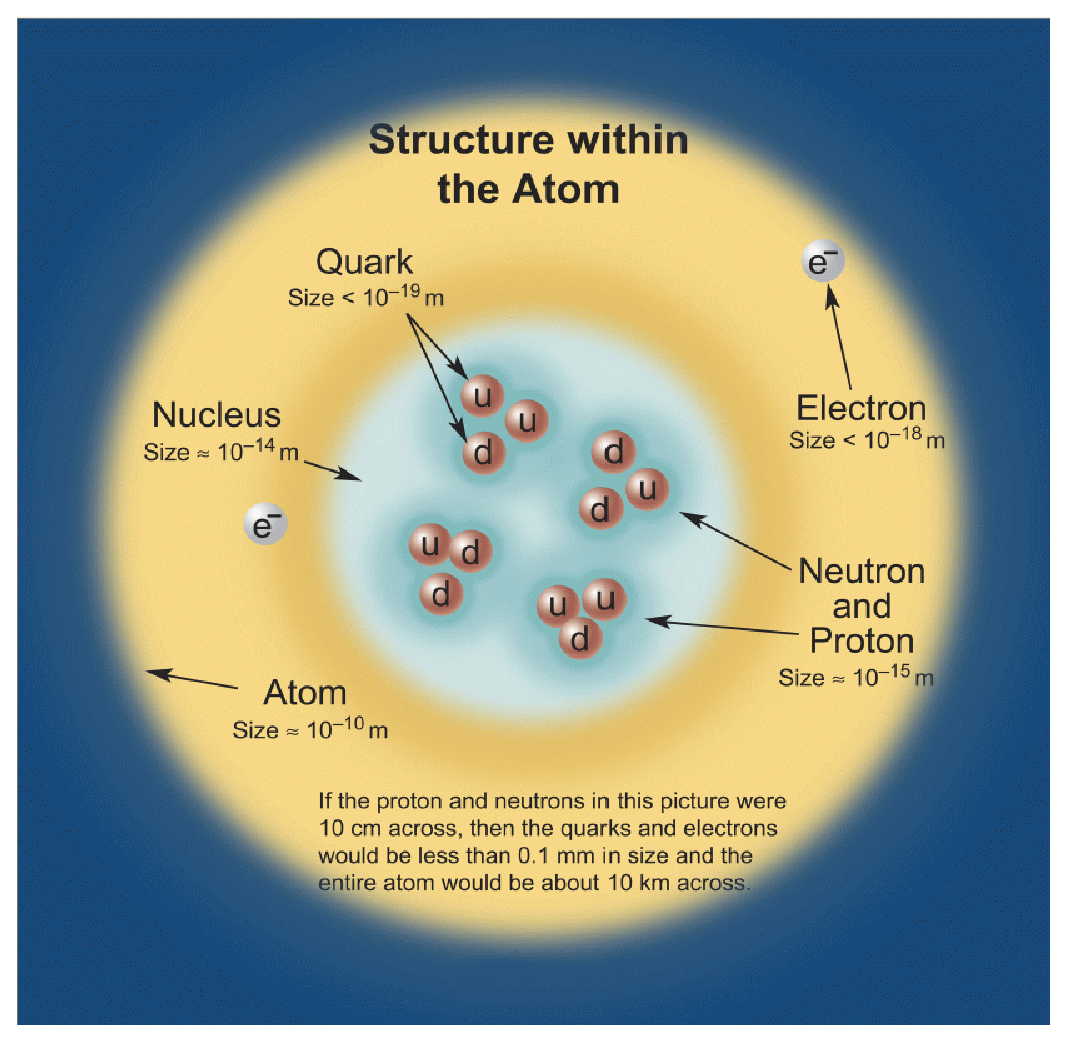
\includegraphics[width=3.2in]{AtomicStructure.ps}

\end{center}

\thispagestyle{empty}

\newpage


\ 
\setcounter{page}{1}

\vfill

Cover art: The atom consists of smaller electrons and a nucleus consisting of protons and neutrons. The protons and neutrons, in turn, are formed from objects called quarks and gluons. Courtesy, the American Institute of Physics.

\pagebreak

\tableofcontents{}


\section{Measuring and Graphing Horizontal Motion\footnote{
1990-93 Dept. of Physics and Astronomy, Dickinson College. Supported by FIPSE
(U.S. Dept. of Ed.) and NSF. Portions of this material have been modified locally
and may not have been classroom tested at Dickinson College.
}}

%{\par\centering Name \rule{2.0in}{0.1pt}\hfill{}Section \rule{1.0in}{0.1pt}\hfill{}Date
%\rule{1.0in}{0.1pt}\par}
\makelabheader %(Space for student name, etc., defined in master.tex or labmanual_formatting_commands.tex)

\textbf{Objectives} 

\begin{itemize} 
\setlength\itemsep{-4pt}
\setlength\topsep{-6pt}
\setlength\partopsep{-6pt}
\vspace{-0.1in}  %There's gotta be a better way to tame this list spacing than this!  --MT
\item To explore the nature of horizontal motion. 
\item To learn to use Excel for graphing and fitting data.
\end{itemize}
\textbf{Measuring the Horizontal Motion of a Bowling Ball} 

A key to understanding how to describe motion near the surface of the earth
is to observe horizontal motions and vertical motions separately. Eventually,
situations in which an object undergoes both horizontal and vertical motion
can be analyzed and understood as a combination of these two kinds of basic
motions.

Let's start with horizontal motion. How do you think the horizontal position
of a bowling ball changes over time as it rolls along on a smooth surface? For
example, suppose you were to roll the ball a distance of 6.0 meters on a fairly
level smooth floor. Do you expect that the ball would: (1) move at a steady
speed, (2) speed up, or (3) slow down? To observe the horizontal motion of a
``bowling ball'' you can use a bocce ball which is slightly
smaller but quite similar to a regulation bowling ball.

\textbf{Apparatus} 

\begin{itemize}\itemsep1pt
\setlength\itemsep{-4pt}
\setlength\topsep{-6pt}
\setlength\partopsep{-6pt}
\vspace{-0.1in}  %There's gotta be a better way to tame this list spacing than this!  --MT
\item A bocce ball 
\item 3 stop watches 
\item A 2-meter stick 
\item Masking tape for marking distances 
\item A smooth level surface (> 7 meters in length)
\end{itemize}
\textbf{Activity 1: Horizontal Motion }

(a) What do you predict will happen to the position of the ball as a function
of time? Will the ball move at a steady speed, speed up, or slow down after
it leaves the bowler's hand? Why?
\vspace{20mm}

(b) Find a 7 meter length of smooth floor and use masking tape to mark off a
starting line and distances of 2.00 m, 4.00 m, and 6.00 m. from the starting
line. Then: (1) Bowl the ball along the surface. (2) Measure the time it takes
to travel 2.0 m, 4.0 m \& 6.0 m. (3) Record the results in the table below.

\textbf{Note:} This is a cooperative project. You will need a bowler, three
people to measure the times, and someone to stop the ball. Practice several
times before recording data in the table below.

\vspace{0.2cm}
{\centering \begin{tabular}{|c|c|}
\hline 
$t$ (s)&
$x$ (m)\\
\hline 
\hline 
0.00&
0.00\\
\hline 
&
\\
\hline 
&
\\
\hline 
&
\\
\hline 
\end{tabular}\par}
\vspace{0.2cm}

(c) Calculate the average speed, $v$, in m/s of the bowling ball as it travels
the 6.00 meters.
\answerspace{20mm}

\pagebreak[2]
\textbf{Activity 2: Drawing a Graph of Position vs. Time}

In this activity, you will graph your data for the position of the ball as
a function of the rolling-time of the ball. This graphing should be done both
by hand and on the computer.

\textbf{NOTE on creating graphs:} Whenever an instruction says ``plot variable 1 as a function of variable 2'', or ``plot variable 1 vs. variable 2'', variable 2 goes on the horizontal axis (independent variable) and variable 1 goes on the vertical axis (dependent variable). Every graph requires a title (like ``Position vs. Time'') and labeled axes with units in parentheses.

(a) Fill in the units and the scale numbers in the graph below and plot the
data you collected, including the (0,0) point listed on the first line of the
above table.

\vspace{0.3cm}
{\par\centering 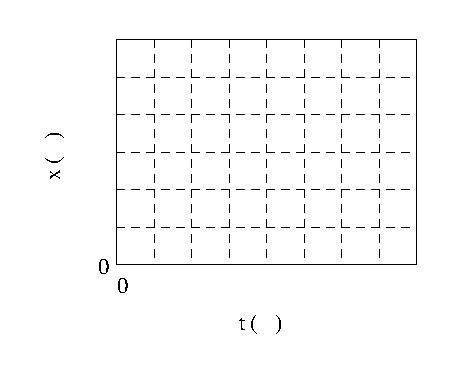
\includegraphics{measuring/measuring_fig1.eps} \par}
\answerspace{0.6cm}

(b) Now use $Excel$ on the computer to create the same graph. Just plot the 
data points; don't try to fit with a line (we will do that in Activity 4). 
See Appendix \ref{excel} for instructions. Print the graph and insert a copy in your 
notebook at the end of this unit.

\textbf{How does the Position of the Ball Vary with Time?} 

We are interested in the mathematical nature of the relationship between position
and time for rolling on a level surface. Some definitions of mathematical relationships
are shown in the sketches below. Figure (a) shows a function $y$ that increases
with $x$ so that $y = f(x)$. 
In sketch (b) $y$ is a linear function that increases
with $x$ so that $y = mx + b$, where 
$m$ is the slope and $b$ is the y intercept. In
figure (c) $y$ is proportional to $x$ ($y = mx$ where $b = 0$).

\answerspace{0.3cm}
{\par\centering 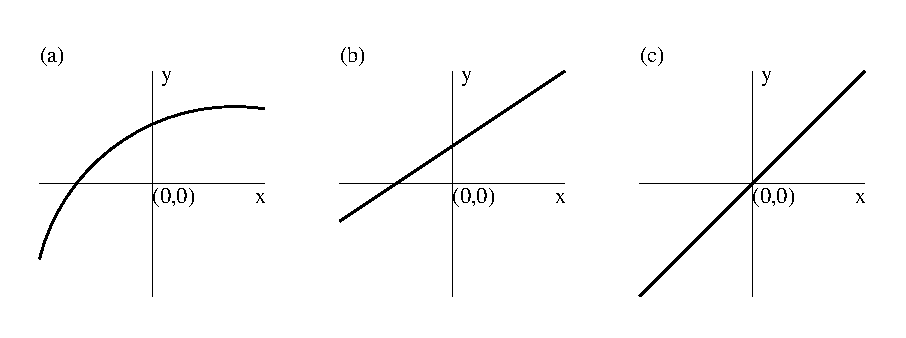
\includegraphics{measuring/measuring_fig2.eps} \par}
\answerspace{0.8cm}

\pagebreak[3]
\textbf{Activity 3: The Mathematical Relationships} 

(a) By comparing the shape of the graph you have just produced with the sketches
shown above, would you say that the position, $x$, increases with time, 
$t$? Decreases
with time? Is it a linear function of $t$? Is it proportional to $t$? Explain.
\vspace{20mm}

(b) How do the results compare with the prediction you made in Activity 1? Are
you surprised?
\vspace{20mm}

(c) What do you think would happen to the slope, $m$, of the graph, if the ball
had been rolled faster? Would it increase? Decrease? Stay the same?
\vspace{20mm}

\textbf{Activity 4: Mathematical Modeling} 

(a) Create a mathematical model of the bocce ball motion data you collected
in Activity 1. This can be done by using $Excel$ to fit the data with
a line. Use a linear fit for this process, and tell the computer to print
the equation for the line. See Appendix \ref{excel} for instructions. 
Be sure to label the graph with a title and axis labels with units. Then print
the graph and include it with this unit.
Does the line provide a good description of the data?
\answerspace{20mm}

(b) Write the equation describing the motion in the form Position $x$ = $vt$ + 
$x_{o}$, using the numbers from the equation of your graph.  Be sure to include units.
\answerspace{20mm}

(c) Use the LINEST function in $Excel$ (see Appendix \ref{excel}) to determine the slope 
$v$ of the line and the uncertainty \( \Delta  v\) in the slope.  Then write 
the velocity as $v$ = slope \( \pm \ \Delta  \)slope, rounding off the numbers as appropriate.  Be sure to include units.
\answerspace{30mm}

\pagebreak[2]
(d) Does the speed you determined in Activity 1 fall within your range of velocity values?  How would you account for any variation?
\answerspace{30mm}

\textbf{Homework} 

The diagram below shows the graphs of three possible relationships between the
time, $t$, in seconds and the position, $x$, in centimeters that the object has
traveled.

\vspace{0.3cm}
{\par\centering 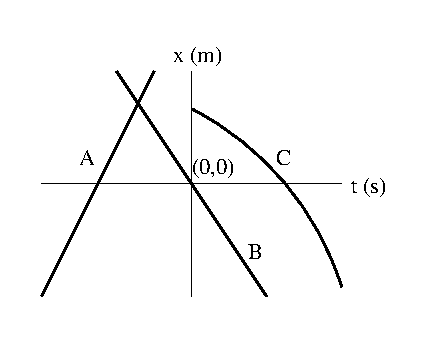
\includegraphics{measuring/measuring_fig3.eps} \par}
\vspace{0.3cm}

(a) Which graphs represent position as a linear function of time? A, B, and/or
C?
\answerspace{10mm}

(b) Which graphs, if any, show position as proportional to time?
\answerspace{10mm}



\section{Walking Speed}

Name \rule{2.0in}{0.1pt}\hfill{}Section \rule{1.0in}{0.1pt}\hfill{}Date \rule{1.0in}{0.1pt}

\textbf{Objectives}

\begin{itemize}
\item Introduction to measuring length and time.
\item Introduction to metric units of length. 
\end{itemize}
\textbf{Apparatus}

\begin{itemize}
\item stop watch
\item 2-meter stick
\end{itemize}
\textbf{Activity}

(a) Use the stop watch and meter stick to determine your walking speed in m/s.

walking speed \rule{2.0in}{0.1pt}

(b) Describe the technique you used to perform the measurement and show the calculation of walking speed.
\vspace{30mm}

(c) Use the stop watch and meter stick to determine your partner's walking speed in m/s.

walking speed \rule{2.0in}{0.1pt}  How does this compare with his/her result?
\vspace{20mm}

\textbf{Question}

What sort of unit is speed (fundamental or derived)?



%
\section{Converting Units}

Name \rule{2.0in}{0.1pt}\hfill{}Section \rule{1.0in}{0.1pt}\hfill{}Date \rule{1.0in}{0.1pt}

{\noindent \bf Objectives:} \begin{list}{$\bullet$}{\itemsep0pt \parsep0pt}

\item Introduction to units \item Exploration of relations between different systems of measurement

\end{list}

{\noindent \bf Apparatus:} \begin{list}{$\bullet$}{\itemsep0pt \parsep0pt}

\item string \item scissors \item meter stick

\end{list}

{\noindent \bf Activity:} \begin{enumerate}

\item Cut the string into three pieces, 1-meter, 1-foot, and 30-cm, respectively.

\item Compare them. Enter into the table below how many lengths of one piece it requires to make each of the others.

\item Cut a length of string equivalent to your anatomical foot; compare this piece to the others.

\begin{center} \begin{tabular}{|l|c|c|c|c|c|} \hline \multicolumn{2}{|c||}{} & \multicolumn{4}{c|}{\bf equal one of these?} \\ \hline \multicolumn{1}{|c}{}& \multicolumn{1}{c||}{pieces}& 1-meter &1-foot & 30-cm & anatomical foot \\ \hline \hline {\bf How} & \multicolumn{1}{c||}{1-meter} &&&& \\ \cline{2-6} {\bf many} & \multicolumn{1}{c||}{1-foot} &&&& \\ \cline{2-6} {\bf of} & \multicolumn{1}{c||}{30-cm} &&&& \\ \cline{2-6} {\bf these} & \multicolumn{1}{c||}{anatomical foot} &&&& \\ \hline \end{tabular} \end{center}

\item Devise your own measurement system; name it; select length, mass, and time standards and choose names and abbreviations for them; and define these.

\begin{center} system name \rule{3in}{0.2pt} \end{center} \begin{tabbing} length: \= name \rule{1in}{0.2pt} \= abbreviation \rule{0.5in}{0.2pt} \= definition \rule{1.5in}{0.2pt} \\ mass: \> name \rule{1in}{0.2pt} \> abbreviation \rule{0.5in}{0.2pt} \> definition \rule{1.5in}{0.2pt} \\ time: \> name \rule{1in}{0.2pt} \> abbreviation \rule{0.5in}{0.2pt} \> definition \rule{1.5in}{0.2pt} \end{tabbing}

\item Compare your measurement system to the Standard International (MKSA) system.

\begin{tabbing} 1 \ \rule{1in}{0.2pt} \= = \= \rule{0.25in}{0.2pt} \ \= meters \kill 1 meter \> = \> \rule{0.25in} {0.2pt} \ \> \rule{1in}{0.2pt}s \\ 1 kilogram \> = \> \rule{0.25in} {0.2pt} \ \> \rule{1in}{0.2pt}s \\ 1 second \> = \> \rule{0.25in} {0.2pt} \ \> \rule{1in}{0.2pt}s \\ 1 \ \rule{1in}{0.2pt} = \rule{0.25in}{0.2pt} \ meters \\ 1 \ \rule{1in}{0.2pt} = \rule{0.25in}{0.2pt} \ kilograms \\ 1 \ \rule{1in}{0.2pt} = \rule{0.25in}{0.2pt} \ seconds \end{tabbing}

\end{enumerate}

\pagebreak

\textbf{Questions: }

1. Are anatomical units practical for measurement? Explain. 
\vspace{20mm}

2. What criteria should be satisfied by a good clock? 
\vspace{20mm}

3. Can you explain the nearly universal use of the metric system in scientific
work?



%
\section{Measurement of Length, Mass, Volume, and Density}

Name \rule{2.0in}{0.1pt}\hfill{}Section \rule{1.0in}{0.1pt}\hfill{}Date \rule{1.0in}{0.1pt}

{\noindent \bf Objectives:} \begin{list}{$\bullet$}{\itemsep0pt \parsep0pt}

\item Learn to measure length with the vernier caliper and mass with the platform balance \item Apply knowledge of units and significant figures \item Understand the dependence of mass and density on dimensions

\end{list}

{\noindent \bf Apparatus:} \begin{list}{$\bullet$}{\itemsep0pt \parsep0pt}

\item vernier caliper \item platform balance \item set of wooden disks

\end{list}

{\noindent \bf Activity:} \begin{enumerate}

\item Find the dimensions in centimeters of each of the disks using the vernier caliper (see Appendix E). Use the averages of three trials for each dimension (diameter, $D$; width, $W$) in the calculations of the volumes ($V = \pi r^2 W$).

\item Find the mass, $M$, of each disk using the laboratory balance.

\item Calculate the density, $\rho$.

\begin{center} \begin{tabular}{|c|c|c|c|c|c|c|c|c|c|c|c|} \hline \multicolumn{1}{|c||}{} & $D_1$ & $D_2$ & $D_3$ & $W_1$ & $W_2$ & $W_3$ & $D$ & $W$ & $V$ & $M$ & $\rho$\\ \multicolumn{1}{|c||}{disk} & (cm) & (cm) & (cm) & (cm) & (cm) & (cm) & (cm) & (cm) & (cc) & (g) & (g/cc) \\ \hline \hline \multicolumn{1}{|c||}{1} & & & & & & & & & & & \\ \hline \multicolumn{1}{|c||}{2} & & & & & & & & & & & \\ \hline \multicolumn{1}{|c||}{3} & & & & & & & & & & & \\ \hline \multicolumn{1}{|c||}{4} & & & & & & & & & & & \\ \hline \multicolumn{1}{|c||}{5} & & & & & & & & & & & \\ \hline \end{tabular} \end{center}

\item Graph mass versus radius and mass versus radius squared.

\end{enumerate}

\pagebreak

{\noindent \bf Questions:}

1. How does the density depend on the size of a disk? 
\vspace{20mm}

2. What is the nature of the relationship between mass and radius? What is the
dependency? 
\vspace{20mm}

3. What is the smallest part of a centimeter that can be read or estimated with
a meter stick? With a vernier caliper? Which reading is more reliable? Explain.
\vspace{20mm}

4. When determining the volume of a disk, which dimension, diameter or width,
should be measured more carefully? Explain. 
\vspace{20mm}

5. What is the volume of the largest disk in cubic millimeters? In liters? What
is its mass in kilograms?



%
\section{Determining $\pi$}

\makelabheader %(Space for student name, etc., defined in master.tex or labmanual_formatting_commands.tex)

{\noindent \bf Objectives:}

\begin{list}{$\bullet$}{\itemsep0pt \parsep0pt}

\item Determine the relationship between circumference and diameter \item Understand the meaning of $\pi$

\end{list}

\textbf{Apparatus:}

\begin{itemize}
\item Wooden disks
\item Meter stick
\item String
\end{itemize}
{\noindent \bf Activity:}

\begin{enumerate}

\item With a meter stick, measure the diameter of one of the disks. Enter the value (or an average of several such measurements) in the table below.

\item With a string and meter stick, measure the circumference of the same disk, and enter the value (or average of several measurements) in the table below.

\item Repeat the previous steps 1. and 2. for each of the disks.

\begin{center} \begin{tabular}{|c|c|c|} \hline disk & diameter (cm) & circumference (cm) \\ \hline\hline 1 & & \\ \hline 2 & & \\ \hline 3 & & \\ \hline 4 & & \\ \hline 5 & & \\ \hline \end{tabular} \end{center}

\item Graph circumference versus diameter using your measurement data.

\item Fit data and determine the slope of the resulting line. \end{enumerate}

\vspace{10pt}

slope \rule{1.5in}{0.2pt}

\vspace{10pt}

{\noindent \bf Questions:}

1. What quantity is identified with the slope of the graph? 
\vspace{10mm}

2. Must the line go through the origin? Explain. 
\vspace{20mm}

3.If the diameter of the largest disk increased by a factor of 2.7, by how much
would its circumference change? 
\vspace{20mm}

4. If you formed a circle with a string 15 mm shorter than the circumference
of the smallest disk, its diameter would be how much smaller than the disk's?



%
\section{Measurement, Uncertainty, and Variation\footnote{
1990-93 Dept. of Physics and Astronomy, Dickinson College. Supported by FIPSE
(U.S. Dept. of Ed.) and NSF. Portions of this material may have been modified
locally and may not have been classroom tested at Dickinson College.
}}

\makelabheader %(Space for student name, etc., defined in master.tex or labmanual_formatting_commands.tex)

\textbf{Objectives }

\begin{itemize}
\item To explore the mathematical meaning of the standard deviation and standard error
associated with a set of measurements. 
\item To investigate random and systematic variations associated with a set of measurements.
\end{itemize}
\textbf{Statistics - The Inevitability of Uncertainty }

With care and attention, it is commonly believed that both mistakes and systematic
errors can be eliminated completely. However, inherent uncertainties do not
result from mistakes or errors. Instead, they can be attributed in part to the
impossibility of building measuring equipment that is precise to an infinite
number of significant figures. The ruler provides us with an example of this.
It can be made better and better, but it always has an ultimate limit of precision.

Another cause of inherent uncertainties is the large number of random variations
affecting any phenomenon being studied. For instance, if you repeatedly drop
a baseball from the level of the lab table and measure the time of each fall,
the measurements will most probably not all be the same. Even if the stop watch
was gated electronically so as to be as precise as possible, there would be
small fluctuations in the flow of currents through the circuits as a result
of random thermal motion of atoms and molecules that make up the wires and circuit
elements. This could change the stop watch reading from measurement to measurement.
The sweaty palm of the experimenter could cause the ball to stick to the hand
for an extra fraction of a second, slight air currents in the room could change
the ball's time of fall, vibrations could cause the floor to oscillate up and
down an imperceptible distance, and so on.

\textbf{Repeated Time-of-Fall Data} 

In the first two activities, you and your partners will take repeated data on
the time of fall of a ball and study how the data vary from some average value
for the time-of-fall.

\textbf{Apparatus} 

\begin{itemize}
\item A ball 
\item A stop watch 
\item A 2-meter stick
\end{itemize}
\textbf{Activity 1: Timing a Falling Ball} 

(a) Drop the ball so it falls through a height of exactly 2.0 m at least 10
times in rapid succession and measure the time of fall in each case. Be as exact as possible about the height from which you drop the ball. Record your 10 time values here:
\vspace{50mm}

(b) Enter your data as a single column in Excel and find the 
average (mean) of the data.
See \textbf{Appendix \ref{excel}} for instructions. Report the
mean value in the space below (including units).
\vspace{10mm}

\textbf{The Standard Deviation as a Measure of Uncertainty }

How certain are we that the average fall-time determined in the previous activity
is accurate? The average of a number of measurements does not tell the whole
story. If all the times you measured were the same, the average would seem to
be very precise. If each of the measurements varied from the others by a large
amount, we would be less certain of the meaning of the average time. We need
criteria for determining the certainty of our data. Statisticians often use
a quantity called the standard deviation as a measure of the level of uncertainty
in data. The standard deviation is usually represented by the Greek letter \( \sigma  \)
(sigma). A customary way of expressing an experimentally determined value is:
Mean  \( \pm \ \sigma  \). The formal mathematical definition of \( \sigma  \)
can be found in \textbf{Appendix \ref{treatment}}.

In the next activity you will use Excel (see \textbf{Appendix \ref{excel}}) to calculate
the value of the standard deviation for the repeated fall-time data you just
obtained and explore how the standard deviation is related to variation in your
data. In particular, you will try to answer this question: What percentage of
your data lies within one standard deviation of the average you calculated?

\textbf{Activity 2: Standard Deviation} 

(a) Report the value for the standard deviation of your data in the space below (including units).
\vspace{10mm}

(b) Calculate the average plus the standard deviation, \(\langle t\rangle 
+ \sigma  \),
and the average minus the standard deviation, \(\langle t\rangle - \sigma  \), 
and record
the results in the space below (including units).
\vspace{10mm}

(c) Determine the number of your data points that lie within \( \pm \sigma  \)
of the average and write the result in the space below. Also, calculate the
percentage of data points lying within a standard deviation of the average and
report that result.
\vspace{10mm}

(d) Combine your results with those obtained by the other groups in the class
and create a table in the space below with the following column headings: Lab
Station, \( \langle t\rangle\) (s), \( \sigma  \) (s), \%Data \( \pm \sigma  \).
\vspace{50mm}

(e) Study the last column, which represents the percentage of data points lying
within one standard deviation of the average. What does the standard deviation,
\( \sigma  \), tell you about the approximate probability that another measurement
will lie within \( \pm \sigma  \) of the average?
\vspace{20mm}

\textbf{Systematic Error - How About the Accuracy of Your Timing Device and
Timing Methods?} 

As the result of problems with your measuring instrument or the procedures you
are using, each of your measurements may tend to be consistently too high or
too low. If this is the case, you probably have a source of systematic error.
There are several types of systematic error.

Most of us have set a watch or clock only to see it gain or lose a certain amount
of time each day or week. In ordinary language we would say that such a time
keeping device is inaccurate. In scientific terms, we would say that it is subject
to systematic error. In the case of a stopwatch or digital timer that doesn't
run continuously like a clock, we have to ask an additional set of questions.
Does it start up immediately? Does it stop exactly when the event is over? Is
there some delay in the start and stop time? A delay in starting or stopping
a timer could also cause systematic error.

Finally, systematic error can be present as a result of the methods you and
your partner are using for making the measurement. For example, are you starting
the timer exactly at the beginning of the event being measured and stopping
it exactly at the end? Are you dropping the ball from a little above the exact
starting point each time? A little below?

\textbf{Activity 3: Is There Systematic Error in the Data? }

We will now use your data set to determine the acceleration due to gravity $g$ 
\underline{and} an uncertainty in the value obtained. As shown in your text, 
the distance $h$ that a ball falls in time $t$ (starting from rest) near the 
earth's surface is given by
\[
h=\frac{1}{2}gt^{2}\]


where $g$ is the acceleration due to gravity. In this idealized equation the 
effects of air resistance have been neglected. 

(a) \underline{Assume} an uncertainty \(\Delta h\) in the height $h$ from 
which you dropped the ball. 
Write $h$ as $h$ \(\pm\ \Delta h\):
\vspace{5mm}

(b) Assume the uncertainty in your average time of fall is the standard 
deviation \( \sigma  \) that you found in Activity 2. Write the time of fall 
as $t$ \(\pm\ \sigma  \):
\vspace{5mm}

(c) Now calculate $g$ from the above equation.
\vspace{15mm}

(d) Next calculate the uncertainty in $g$ from

$$
\frac{\Delta g}{g} = \sqrt{\left(\frac{\Delta h}{h}\right)^2 + \left(\frac{2\Delta t}{t}\right)^2}
$$
\vspace{15mm}

Write $g$ as $g$ \(\pm\ \Delta g\):

Does the ``accepted value'' of $g$ (9.80 m/s$^2$) fall within the range of 
values you have determined for $g$? If not, you probably have a source of 
systematic error.

(e) If you seem to have systematic error, explain whether the measured times
tend to be too short or too long and list some of the possible causes of it
in the space below.
\vspace{30mm}

\textbf{Activity 4: Visualizing Your Data}

In Activities 1-2 you extracted the mean and standard deviation for your data set. 
These two numbers characterize your data, but they contain far less information than the full
data set.
To pull more understanding from your data we want to investigate a common method for
creating a pictorial representation of your data: the histogram.
A histogram is a summary graph showing a count of your data points falling in various ranges. 
The effect is a rough approximation of the frequency distribution of the data showing you how often different outcomes might occur.
You may be familiar with histograms from seeing distributions of grades on an exam.
The histogram you are about to make is analogous to such a grade distribution except you will be using your measured fall times
instead of student grades.

(a) Follow the instructions in \textbf{Appendix \ref{excel}} to make a histogram of your data. 
One of the choices you have to make in producing the histogram is the size and position of the `bins'.
The horizontal range of your data will be broken up into a series of adjacent sub-ranges that will be used
to sort your data. The bin size is simply the length of each sub-range. 
We will typically use a constant bin size.
For your initial bin size divide your standard deviation from Activity 2 by about three or so and use that number when you follow the directions in
\textbf{Appendix \ref{excel}}.
Once you have made the histogram, print it, and attach it to this unit.
\vspace{2mm}

(b) How many peaks are in your histogram? Explain your reasoning.
\vspace{10mm}

(c) What does the histogram of the fall-times data tell you?
\vspace{15mm}

(d) Do the average and standard deviation capture the full description of your data? Why or why not.
\vspace{15mm}

(e) Consider the histogram shown below for two sets of possible fall times from different classes. 
The average and standard deviation of the data is $0.95\pm 0.36 ~ s$. How many peaks are in this
histogram? Do the average and standard deviation capture the full description of the data? Why or why not.

\begin{figure}[hb]
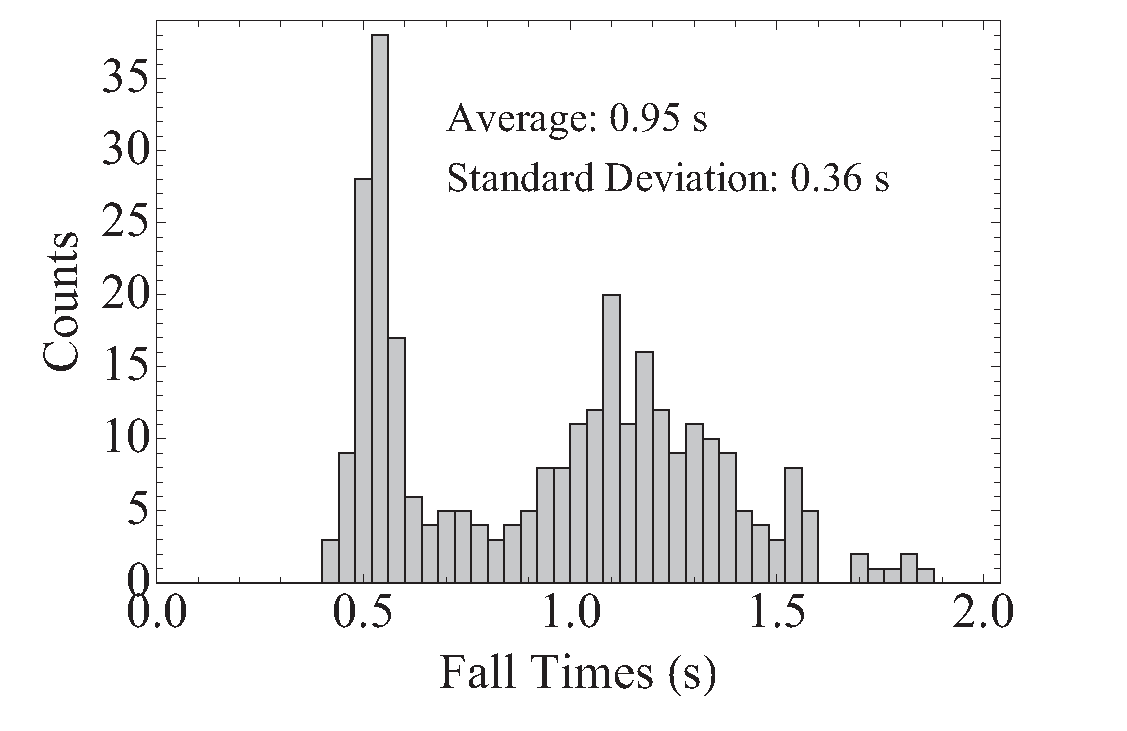
\includegraphics[height=2.25in]{measurement_uncertainty/SampleHist1_bw.eps}\label{SampleHist1}
\end{figure}

(f) What advantages do histograms have over the average and standard deviation?
\vspace{20mm}

\newpage


\textbf{Homework} 

1. Suppose you made the following five length measurements of the width of a
piece of $8\frac{1}{2} {}''\, \times 11''$ paper which has been cut carefully by
a manufacturer using an unfamiliar centimeter rule: 21.33 cm, 21.52 cm, 21.47
cm, 21.21 cm, 21.45 cm. (a) Find the mean and standard deviation of the measurements.
The formal mathematical definition of standard deviation 
is given in Appendix \ref{treatment}. 
\vspace{30mm}

(b) Is there any evidence of uncertainty in the measurements or are they precise?
Explain. 
\vspace{20mm}

(c) Is there any evidence of systematic error in the measurements? If so, what
might cause this? Explain.
\vspace{20mm}

2. Suppose Ashley and Ryan each throw darts at targets as shown below. Each
of them is trying very hard to hit the bulls eye each time. Discuss in essay
form which of the two students has the least amount of random
error associated with his
or her throws and is thus more precise. Is one of the students less accurate
is the sense of having a systematic error associated with his or her throws?
What factors like eyesight and coordination might cause one to be more precise
and another more accurate?

\vspace{0.3cm}
{\par\centering 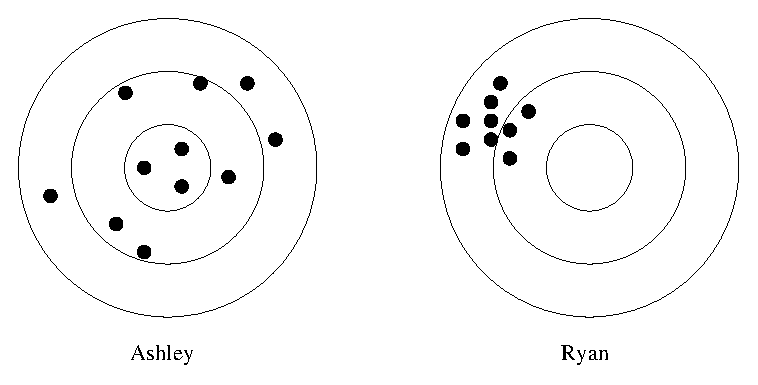
\includegraphics{measurement_uncertainty/measurement_uncertainty_fig1.eps} \par}
\vspace{0.3cm}




\section{Position \textit{vs.}~Time Graphs\footnote{
1990-93 Dept. of Physics and Astronomy, Dickinson College. Supported by FIPSE
(U.S. Dept. of Ed.) and NSF. Portions of this material may have been modified
locally and may not have been classroom tested at Dickinson College.
}}

\makelabheader %(Space for student name, etc., defined in master.tex or labmanual_formatting_commands.tex)

\bigskip

\textbf{Objectives} 

\begin{itemize}[nosep]
\item To learn about two of the ways that physicists can describe motion in one dimension-words
and graphs. 
\item To learn how to relate graphs of position \textit{vs.}~time to the motions they represent.
\end{itemize}

\bigskip

\textbf{Apparatus} 

\begin{itemize}[nosep]
\item Pasco 550 Interface
\item Ultrasonic motion detector 
\item \textit{Capstone} software (\filename{P\_Graphs.cap} experiment file)
\item Wooden board
\item Masking tape for marking distances
\end{itemize}

\bigskip

\textbf{Introduction} 

The focus of this unit on kinematics is to be able to describe your position
as a function of time using words and graphs. You will use a motion detector
attached to a computer in the laboratory to learn to describe one-dimensional
motion.

The ultrasonic motion detector sends out a series of sound pulses that are of
too high a frequency to hear. These pulses reflect from objects in the vicinity
of the motion detector and some of the sound energy returns to the detector.
The computer is able to record the time it takes for reflected sound waves to
return to the detector and then, by knowing the speed of sound in air, figure
out how far away the reflecting object is. There are several things to watch
out for when using a motion detector. (1) Do not get closer than 0.15 meters
from the detector because it cannot record reflected pulses which come back
too soon. (2) The ultrasonic waves come out in a cone of about 15\( ^{\circ } \).
It will see the closest object. Be sure there is a clear path between the object
whose motion you want to track and the motion detector. (3) The motion detector
is very sensitive and will detect slight motions. You can try to glide smoothly
along the floor, but don't be surprised to see small bumps in velocity graphs.
(4) Some objects like bulky sweaters are good sound absorbers and may not be
``seen'' well by a motion detector. Hold a wooden board in front of you when 
doing the activities below so the motion detector can see a smooth surface.

\textbf{Position \textit{vs.}~Time Graphs of Your Motion }

The purpose of this unit is to learn how to relate graphs of position as a function
of time to the motions they represent. How does a position \textit{vs.}~time graph look
when you move slowly? Quickly? What happens when you move toward the motion
detector? Away? After completing the next few activities, you should be able
to look at a position \textit{vs.}~time graph and describe the motion of the object.
You should also be able to look at the motion of an object and sketch a graph
representing that motion.

Note that the motion detector measures the distance of an object from the detector,
and that the motion detector is located at the origin of each graph. It is common
to refer to the distance of an object from some origin as the position of the
object. Therefore, it is better to refer to these graphs as position \textit{vs.}~time
graphs than distance \textit{vs.}~time graphs.

You will use the \textit{Capstone} software to do the following activities.
Launch the \filename{P\_Graphs.cap} file by going to the \filename{\coursefolder} folder on the desktop. 
To start a data run, click the \textbf{Record} button. To stop a data run,
click the \textbf{Stop} button. After a data run, the graph can be expanded
by clicking on the \textbf{Scale to fit} button in the upper left corner of
the Graph window. Multiple data sets can be displayed on the same graph. Data
can be removed from the graph by opening the \textbf{Delete Last Run} menu on the \textbf{Controls} palette 
 (at bottom of screen) and selecting \textit{delete all runs} or \textit{delete run number x}.
  When you are finished with the activities, choose \textbf{Exit} from the \textbf{File} menu
and do not save this activity.

Before you begin the activities, you should mark a position scale on the floor.
To do this, position one person at approximately 1 meter in front of the motion
detector and take data for 1 second. The computer will display a horizontal
line showing the position measured by the detector. The person standing in front
of the detector should then adjust his/her position and the procedure repeated
until the 1 meter position is established. Mark the 1 meter position on the
floor with a piece of masking tape and then mark the 2, 3 and 4 meter positions
using the 2 meter stick.

\textbf{Activity 1: Making Position \textit{vs.}~Time Graphs }

Make position-time graphs for the following motions and sketch the graph you
observe in each case:

(a) Starting at 0.5 m, walk away from the origin (i.e., the detector) slowly
and steadily.

%\vspace{0.3cm}
%{\par\centering 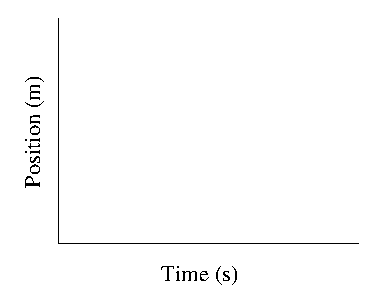
\includegraphics{position/position_fig1.eps} \par}
%\vspace{0.3cm}
\begin{lab_axis}*[lab_noticks_1quad,
	height = {2.0in}, width = {2.5in},
	xlabel={Time},
	ylabel={Position},
	]
\end{lab_axis}

(b) Walk away from the origin medium-fast and steadily.

%\vspace{0.3cm}
%{\par\centering 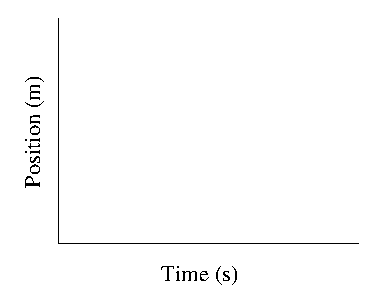
\includegraphics{position/position_fig1.eps} \par}
%\vspace{0.3cm}
\begin{lab_axis}*[lab_noticks_1quad,
	height = {2.0in}, width = {2.5in},
	xlabel={Time},
	ylabel={Position},
	]
\end{lab_axis}

(c) Walk toward the detector (origin) slowly and steadily.

%\vspace{0.3cm}
%{\par\centering 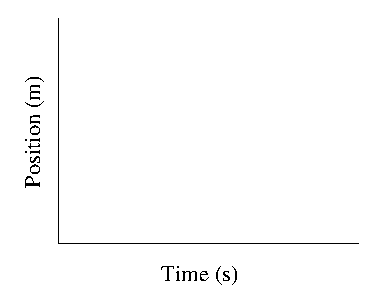
\includegraphics{position/position_fig1.eps} \par}
%\vspace{0.3cm}
\begin{lab_axis}*[lab_noticks_1quad,
	height = {2.0in}, width = {2.5in},
	xlabel={Time},
	ylabel={Position},
	]
\end{lab_axis}

(d) Describe the difference between the graph you made by walking away slowly
and the one made by walking away more quickly.
\answerspace{20mm}

(e) Describe the difference between the graph made by walking toward and the
one made walking away from the motion detector.
\answerspace{20mm}

\textbf{Activity 2: Predicting a Position \textit{vs.}~Time Graph} 

(a) Suppose your were to start 1.0 m in front of the detector and walk away
slowly and steadily for 4 seconds, stop for 4 seconds, and then walk toward
the detector quickly. Sketch your prediction on the axes below using a dashed
line.

%\vspace{0.3cm}
%{\par\centering 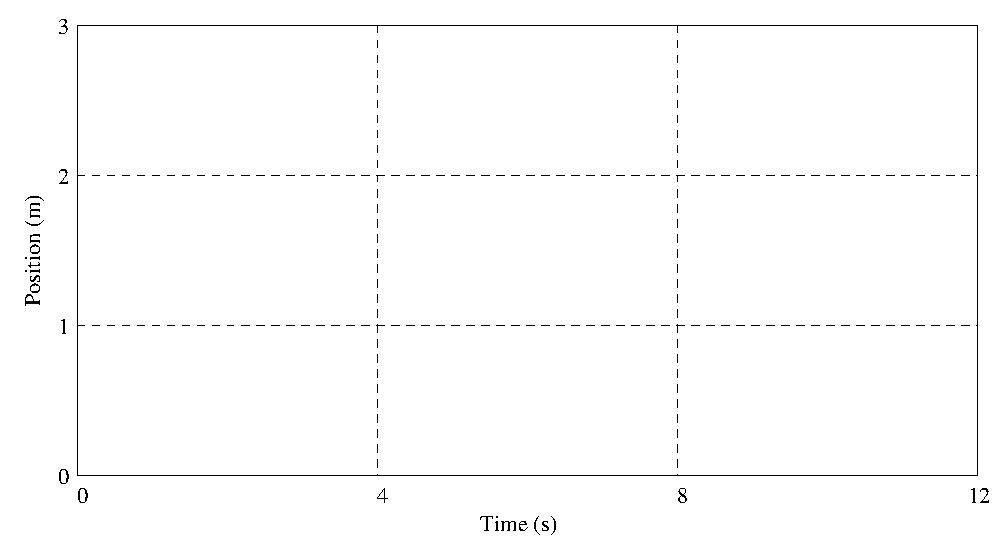
\includegraphics{position/position_fig2.eps} \par}
%\vspace{0.3cm}
\begin{lab_axis}*[lab_grid,
	height = {3in},
	width = {6in},
	xlabel={Time (s)},
	ylabel={Position (m)},
	xmin=0, xmax=12,
	ymin=0, ymax=3,
	xtick distance = 4,
%	ytick distance = 1,
	minor y tick num=1,
	minor x tick num=3,
	]
\end{lab_axis}

(b) Test your prediction by moving in the way described and making a graph of
your motion with the motion detector. Sketch the trace of your actual motion
on the above graph with a solid line. 

(c) Is your prediction the same as the final result? If not, describe how you
would move to make a graph that looks like your prediction.
\answerspace{20mm}

\pagebreak[2]
\textbf{Activity 3: Matching Position \textit{vs.}~Time Graphs}

%\vspace{0.3cm}
%{\par\centering 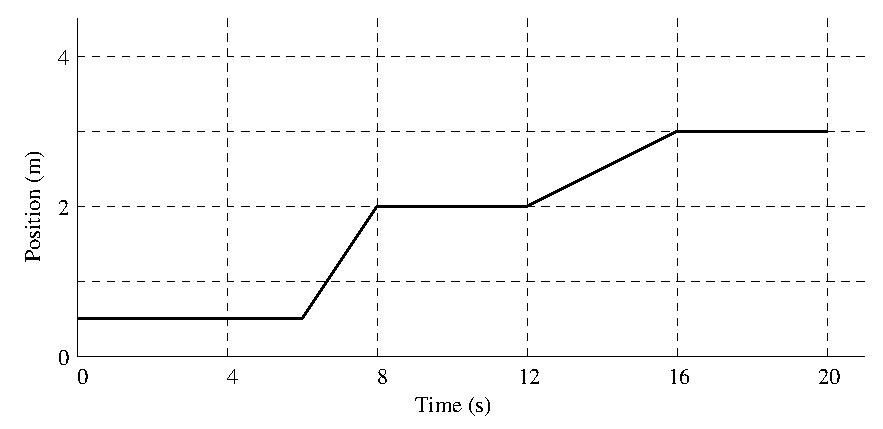
\includegraphics[width=0.7\textwidth]{position/position_fig3.eps} \par}
%\vspace{-0.1cm}
\begin{lab_axis}*[lab_grid,
	height = {2.5in},
	width = {5in},
	xlabel={Time (s)},
	ylabel={Position (m)},
	xmin=0, xmax=20,
	ymin=0, ymax=4,
	xtick distance = 4,
	ytick distance = 2,
	minor y tick num=1,
	minor x tick num=1,
	]
\addplot coordinates{(0,0.5) (6,0.5) (8,2) (12,2) (16,3) (20,3)};
\end{lab_axis}

(a) Describe in your own words how you would move in order to match the graph
shown above.
\answerspace{15mm}

(b) Move to match the above graph on the computer screen. You may try a number
of times. It helps to work as a team. Get the times right. Get the positions
right. Do this for yourself. (Each person in your group should do his or her
own match.) You will not learn very much by just watching!

(c) What was the difference in the way you moved to produce the two differently
sloped parts of the graph you just matched?
\answerspace{12mm}

(d) Make curved position \textit{vs.}~time graphs like those shown below.

%\vspace{0.3cm}
%{\par\centering 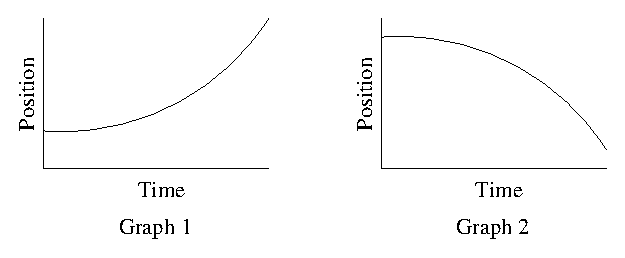
\includegraphics[width=0.5\textwidth]{position/position_fig4.eps} \par}
%\vspace{-0.1cm}
\begin{center}
\begin{lab_axis}[lab_noticks_1quad,
	height = {1.5in}, width = {2in},
	xlabel={Time},
	ylabel={Position},
	title={Graph 1},
	]
\addplot[domain=0:0.9] {0.8*x^2 + 0.2};
\end{lab_axis}
\hspace{0.5in}
\begin{lab_axis}[lab_noticks_1quad,
	height = {1.5in}, width = {2in},
	xlabel={Time},
	ylabel={Position},
	title={Graph 2},
	]
\addplot[domain=0:0.9] {-0.8*x^2 + 0.9};
\end{lab_axis}
\end{center}

%\vspace{-1em} %I don't know why there seems to be some extra space after these graphs. 

(e) Describe how you must move to produce a position \textit{vs.}~time graph with each
of the shapes shown.

Graph 1 answer:
\answerspace{10mm}

Graph 2 answer:
\answerspace{10mm}

\pagebreak[3]
(f) What is the general difference between motions which result in a straight-line
position \textit{vs.}~time graph and those that result in a curved-line position vs.
time graph?
\answerspace{15mm}

\textbf{Homework} 

Answer the following questions in the spaces provided.

1.What do you do to create a horizontal line on a position-time graph?

%\vspace{0.3cm}
%{\par\raggedright 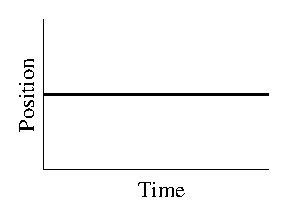
\includegraphics{position/position_fig5.eps} \par}
%\vspace{0.3cm}
\begin{lab_axis}[lab_noticks_1quad,
	height = {1.6in}, width = {2.0in},
	xlabel={Time},
	ylabel={Position},
	]
\addplot[domain=0:0.9] {0.5};
\end{lab_axis}

2. How do you walk to create a straight line that slopes up?

%\vspace{0.3cm}
%{\par\raggedright 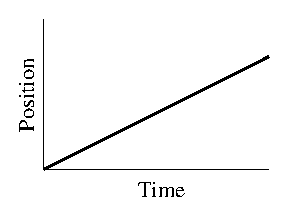
\includegraphics{position/position_fig6.eps} \par}
%\vspace{0.3cm}
\begin{lab_axis}[lab_noticks_1quad,
	height = {1.6in}, width = {2.0in},
	xlabel={Time},
	ylabel={Position},
	]
\addplot[domain=0:0.9] {x};
\end{lab_axis}

3. How do you walk to create a straight line that slopes down?

%\vspace{0.3cm}
%{\par\raggedright 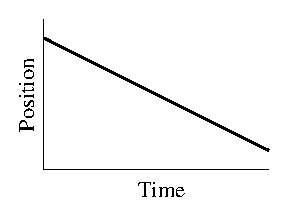
\includegraphics{position/position_fig7.eps} \par}
%\vspace{0.3cm}
\begin{lab_axis}[lab_noticks_1quad,
	height = {1.6in}, width = {2.0in},
	xlabel={Time},
	ylabel={Position},
	]
\addplot[domain=0:0.9] {0.9 - 0.8*x};
\end{lab_axis}

4. How do you move so the graph goes up steeply at first, then continues up
gradually?

%\vspace{0.3cm}
%{\par\raggedright 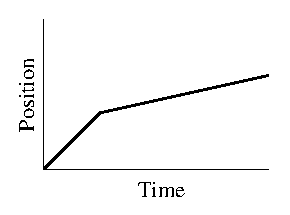
\includegraphics{position/position_fig8.eps} \par}
%\vspace{0.3cm}
\begin{lab_axis}[lab_noticks_1quad,
	height = {1.6in}, width = {2.0in},
	xlabel={Time},
	ylabel={Position},
	]
\addplot coordinates{(0,0) (0.25, 0.4) (0.9,0.7)};
\end{lab_axis}

5. How do you walk to create a U-shaped graph?

%\vspace{0.3cm}
%{\par\raggedright 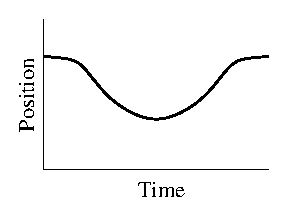
\includegraphics{position/position_fig9.eps} \par}
%\vspace{0.3cm}
\begin{lab_axis}[lab_noticks_1quad,
	height = {1.6in}, width = {2.0in},
	xlabel={Time},
	ylabel={Position},
	]
\addplot [smooth, tension=0.95] coordinates{(0,0.8) (0.2, 0.7) (0.5,0.25) (0.8, 0.7) (1.0, 0.8)};
\end{lab_axis}

\pagebreak[2]
Answer the following about the two objects A and B, whose motion produced
the following position-time graphs.

6. (a) Which object is moving faster? (b) Which starts ahead? Define what you
mean by ``ahead.''

(c) What does the intersection mean?

%\vspace{0.3cm}
%{\par\raggedright 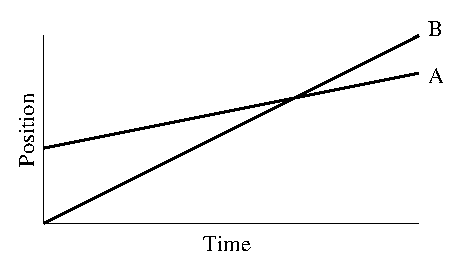
\includegraphics{position/position_fig10.eps} \par}
%\vspace{0.3cm}
\begin{lab_axis}[lab_noticks_1quad,
	height = {1.9in}, width = {2.8in},
	xlabel={Time},
	ylabel={Position},
	]
\addplot coordinates {(0,0.0) (0.9,0.9)} node[right] {B};
\addplot coordinates {(0,0.4) (0.9,0.7)} node[right] {A};
\end{lab_axis}

7. (a) Which object is moving faster? (b) Which object has a negative velocity
according to the convention we have established?

%\vspace{0.3cm}
%{\par\raggedright 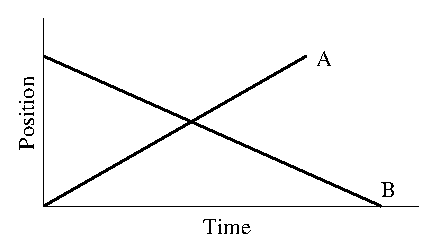
\includegraphics{position/position_fig11.eps} \par}
%\vspace{0.3cm}
\begin{lab_axis}[lab_noticks_1quad,
	height = {1.9in}, width = {2.8in},
	xlabel={Time},
	ylabel={Position},
	]
\addplot coordinates {(0,0.0) (0.9,0.9)} node[right] {A};
\addplot coordinates {(0,0.6) (0.9,0.3)} node[right] {B};
\end{lab_axis}

8. (a) Which object is moving faster? (b) Which starts ahead? Define what you
mean by ``ahead.''

%\vspace{0.3cm}
%{\par\raggedright 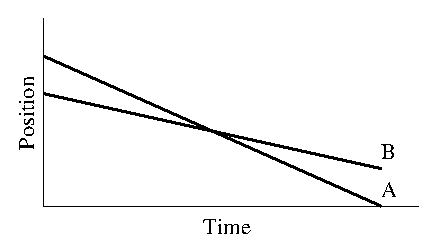
\includegraphics{position/position_fig12.eps} \par}
%\vspace{0.3cm}
\begin{lab_axis}[lab_noticks_1quad,
	height = {1.9in}, width = {2.8in},
	xlabel={Time},
	ylabel={Position},
	]
\addplot coordinates {(0,0.9) (0.9,0.1)} node[right] {A};
\addplot coordinates {(0,0.6) (0.9,0.3)} node[right] {B};
\end{lab_axis}

Sketch the position-time graph corresponding to each of the following descriptions
of the motion of an object.

9. The object moves with a steady (constant) velocity away from the origin.

%\vspace{0.3cm}
%{\par\centering 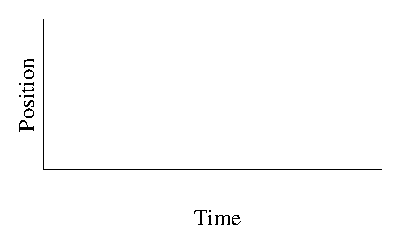
\includegraphics{position/position_fig13.eps} \par}
%\vspace{0.3cm}
\begin{lab_axis}*[lab_noticks_1quad,
	height = {1.8in}, width = {2.8in},
	xlabel={Time},
	ylabel={Position},
	]
\end{lab_axis}

\pagebreak
10. The object is standing still.

\begin{lab_axis}*[lab_noticks_1quad,
	height = {1.8in}, width = {2.8in},
	xlabel={Time},
	ylabel={Position},
	]
\end{lab_axis}

11. The object moves with a steady (constant) velocity toward the origin for
5 seconds and stands still for 5 seconds.

\begin{lab_axis}*[lab_noticks_1quad,
	height = {1.8in}, width = {2.8in},
	xlabel={Time},
	ylabel={Position},
	]
\end{lab_axis}

12. The object moves with a steady velocity away from the origin for 5 seconds,
then reverses direction and moves at the same speed toward the origin for 5
seconds.

\begin{lab_axis}*[lab_noticks_1quad,
	height = {1.8in}, width = {2.8in},
	xlabel={Time},
	ylabel={Position},
	]
\end{lab_axis}

13. The object moves away from the origin, starting slowly and speeding up.

\begin{lab_axis}*[lab_noticks_1quad,
	height = {1.8in}, width = {2.8in},
	xlabel={Time},
	ylabel={Position},
	]
\end{lab_axis}





\section{Velocity \textit{vs.}~Time Graphs\footnote{
1990-93 Dept. of Physics and Astronomy, Dickinson College. Supported by FIPSE
(U.S. Dept. of Ed.) and NSF. Portions of this material may have been modified
locally and may not have been classroom tested at Dickinson College.
}}

\makelabheader %(Space for student name, etc., defined in master.tex or labmanual_formatting_commands.tex)

\bigskip

\textbf{Objectives }

\begin{itemize}[nosep]
\item To acquire an intuitive understanding of speed and velocity in one dimension. 
\item To learn how to relate graphs of velocity \textit{vs.}~time to the motions they represent.
\end{itemize}

\bigskip
\textbf{Apparatus}

\begin{itemize}[nosep]
\item Pasco 550 Interface
\item Ultrasonic motion detector
\item \textit{Capstone} software (\filename{V\_Graph.cap} experiment file)
\item Wooden board
\end{itemize}

\bigskip
\textbf{Introduction} 

You have already plotted your position as a function of time. Another way to
represent your motion during an interval of time is with a graph which describes
how fast and in what direction you are moving from moment to moment. How fast
you move is known as your speed. It is the rate of change of position with respect
to time. Velocity is a quantity which takes into account your speed and the
direction you are moving. Thus, when you examine the motion of an object moving
along a line, its velocity can be positive or negative depending
on whether the object is moving in the positive or negative direction.

Graphs of velocity over time are more challenging to create and interpret than
those for position. A good way to learn to interpret them is to create and examine velocity \textit{vs.}~time graphs of your own body motions, as you will do in the next few activities.

\bigskip

\textbf{Activity 1: Making Velocity \textit{vs.}~Time Graphs} 

To make the graphs in the following activities, open the \filename{V\_Graph.cap} application in the \filename{\coursefolder} folder. Click \textbf{Record} to begin, \textbf{Stop} to end a data run.

(a) Make a velocity graph by walking away from the detector slowly and steadily.
Try again until you get a graph you're satisfied with and then sketch your result
on the graph that follows. (We suggest you draw smooth patterns by ignoring
smaller bumps that are mostly due to your steps.)

%\vspace{0.3cm}
%{\par\centering 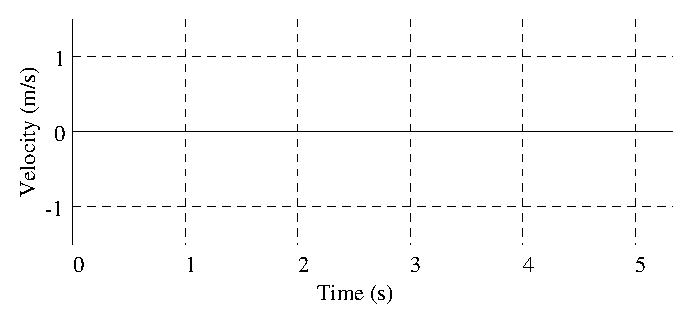
\includegraphics{velocity/velocity_fig1.eps} \par}
%\vspace{0.3cm}
\begin{lab_axis}*[lab_grid,
	height = {2.5in}, width = {5in},
	xlabel={Time (s)},
	ylabel={Velocity (m/s)},
	xmin=0, xmax=5.5,
	ymin=-1.5, ymax=1.5,
	xtick distance = 1,
	ytick distance = 1,
	y0_line,
	]
\end{lab_axis}

(b) Make a velocity graph, walking away from the detector steadily at a medium
speed. Sketch your graph below.

%\vspace{0.3cm}
%{\par\centering 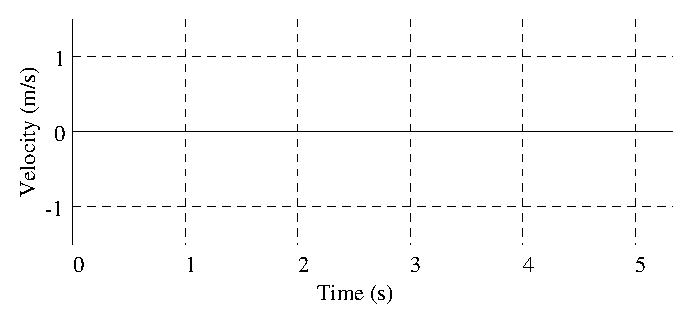
\includegraphics[width=0.7\textwidth]{velocity/velocity_fig1.eps} \par}
%\vspace{0.3cm}
\begin{lab_axis}*[lab_grid,
	height = {2.5in}, width = {5in},
	xlabel={Time (s)},
	ylabel={Velocity (m/s)},
	xmin=0, xmax=5.5,
	ymin=-1.5, ymax=1.5,
	xtick distance = 1,
	ytick distance = 1,
	y0_line,
	]
\end{lab_axis}

(c) Make a velocity graph, walking toward the detector slowly and steadily.
Sketch your graph below.

%\vspace{0.3cm}
%{\par\centering 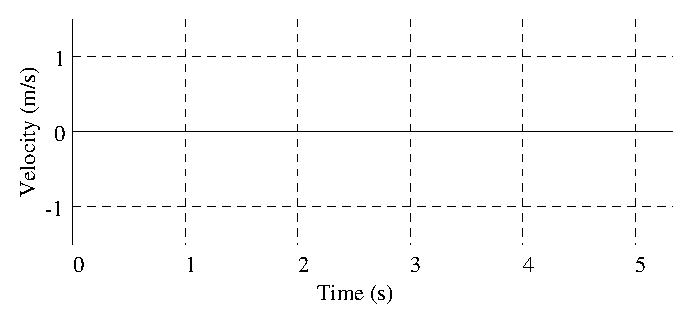
\includegraphics[width=0.7\textwidth]{velocity/velocity_fig1.eps} \par}
%\vspace{0.3cm}
\begin{lab_axis}*[lab_grid,
	height = {2.5in}, width = {5in},
	xlabel={Time (s)},
	ylabel={Velocity (m/s)},
	xmin=0, xmax=5.5,
	ymin=-1.5, ymax=1.5,
	xtick distance = 1,
	ytick distance = 1,
	y0_line,
	]
\end{lab_axis}

(d) What is the most important difference between the graph made by slowly walking
away from the detector and the one made by walking away more quickly? 
\answerspace{25mm}

(e) How are the velocity \textit{vs.}~time graphs different for motion away and motion
toward the detector?
\answerspace{25mm}

\pagebreak[2]
\textbf{Activity 2: Predicting a Velocity \textit{vs.}~Time Graph }

Suppose you were to undergo the following sequence of motions: (1) walk away
from the detector slowly and steadily for 6 seconds, (2) stand still for 6 seconds,
(3) walk toward the detector steadily about twice as fast as before.

(a) Use a dashed line in the graph that follows to record your prediction of
the shape of the velocity graph that will result from the motion described above.

%\vspace{0.3cm}
%{\par\centering 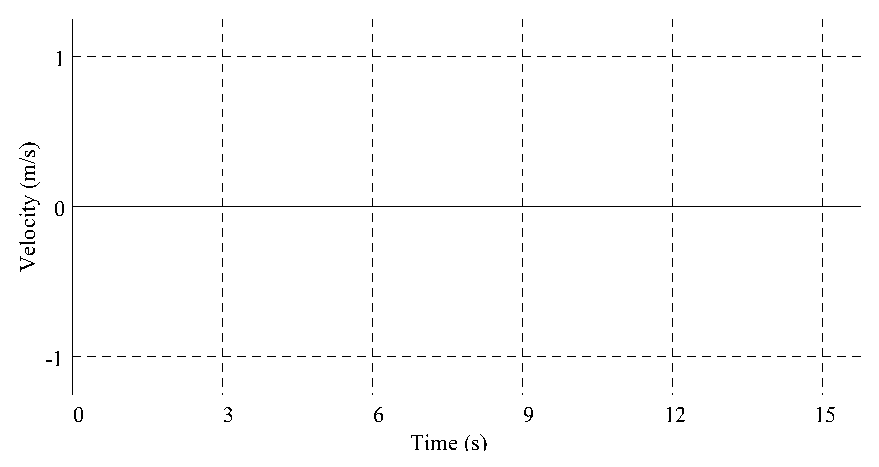
\includegraphics[width=0.7\textwidth]{velocity/velocity_fig2.eps} \par}
%\vspace{0.3cm}
\begin{lab_axis}*[lab_grid,
	height = {2.5in}, width = {5in},
	xlabel={Time (s)},
	ylabel={Velocity (m/s)},
	xmin=0, xmax=16,
	ymin=-1.5, ymax=1.5,
	xtick distance = 3,
	ytick distance = 1,
	y0_line,
	]
\end{lab_axis}

(b) Compare predictions with your partner(s) and see if you can all agree. Use
a solid line to sketch your group prediction in the graph above.

(c) Adjust the sampling time to 15 s and then test your prediction. Repeat your
motion until you are confident that it matches the description in words and
then draw the actual graph on the axes below. Be sure the 6-second stop shows
clearly.

%\vspace{0.3cm}
%{\par\centering 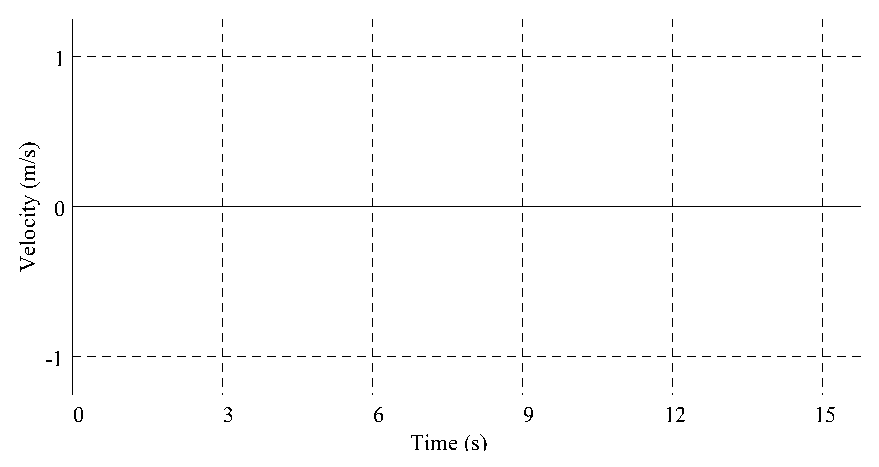
\includegraphics[width=0.7\textwidth]{velocity/velocity_fig2.eps} \par}
%\vspace{0.3cm}
\begin{lab_axis}*[lab_grid,
	height = {2.5in}, width = {5in},
	xlabel={Time (s)},
	ylabel={Velocity (m/s)},
	xmin=0, xmax=16,
	ymin=-1.5, ymax=1.5,
	xtick distance = 3,
	ytick distance = 1,
	y0_line,
	]
\end{lab_axis}

(d) Did your prediction match your real motion? If not, what misunderstanding
of what elements of the graph did you have?
\answerspace{20mm}

\pagebreak[2]
\textbf{Velocity Vectors} 

The two ideas of speed and direction can be combined and represented by vectors.
A velocity vector is represented by an arrow pointing in the direction of motion.
The length of the arrow is drawn proportional to the speed; the longer the arrow,
the larger the speed. If you are moving toward the right, your velocity vector
can be represented by the arrow shown below.

\vspace{0.3cm}
{\par\centering 
\includegraphics{velocity/velocity_fig3.eps} \par}
\vspace{0.3cm}

If you were moving twice as fast toward the right, the arrow representing your
velocity vector would look like:

\vspace{0.3cm}
{\par\centering 
\includegraphics{velocity/velocity_fig4.eps} \par}
\vspace{0.3cm}

while moving twice as fast toward the left would be represented by the following
arrow:

\vspace{0.3cm}
{\par\centering 
\includegraphics{velocity/velocity_fig5.eps} \par}
\vspace{0.3cm}

What is the relationship between a one-dimensional velocity vector and the sign
of velocity? This depends on the way you choose to set the positive $x$-axis.

\vspace{0.3cm}
{\par\centering 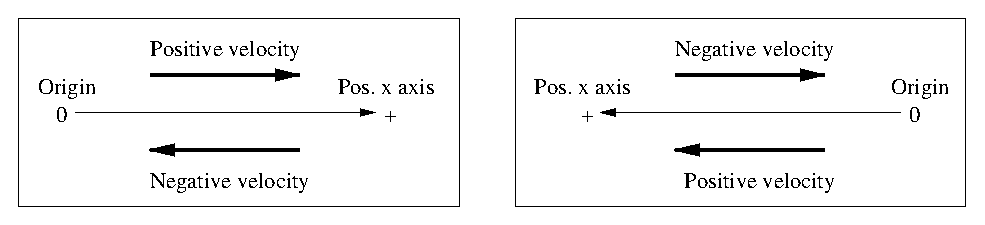
\includegraphics{velocity/velocity_fig6.eps} \par}
\vspace{0.3cm}

In both diagrams the top vectors represent velocity toward the right. In the
left diagram, the $x$-axis has been drawn so that the positive $x$-direction is
toward the right. Thus the top arrow represents positive velocity. However,
in the right diagram, the positive $x$-direction is toward the left. Thus the
top arrow represents negative velocity. Likewise, in both diagrams the bottom
arrows represent velocity toward the left. In the left diagram this is negative
velocity, and in the right diagram it is positive velocity.

\textbf{Activity 3: Sketching Velocity Vectors} 

Sketch below velocity vectors representing the three parts of the motion described
in the prediction you made in Activity 2.

(a)Walking slowly away from the detector:
\answerspace{8mm}

(b) Standing still (just a dot):
\answerspace{8mm}

(c) Walking rapidly toward the detector:
\answerspace{8mm}

\pagebreak[2]
\textbf{Activity 4: Matching a Velocity Graph} 

(a) Describe how you think you will have to move in order to match the velocity
graph shown below.

%\vspace{0.3cm}
%{\par\centering 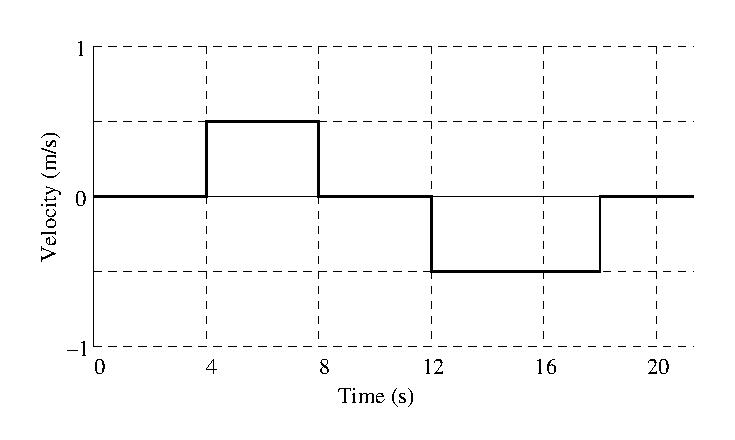
\includegraphics{velocity/velocity_fig7.eps} \par}
%\vspace{0.3cm}
\begin{lab_axis}*[lab_grid,
	height = {2.5in}, width = {5in},
	xlabel={Time (s)},
	ylabel={Velocity (m/s)},
	xmin=0, xmax=22,
	ymin=-1, ymax=1,
	xtick distance = 4,
	ytick distance = 1,
	minor y tick num=1,
	y0_line,
	]
\addplot coordinates {(0,0) (4,0) (4,0.5) (8,0.5) (8,0) (12,0) (12,-0.5) (18,-0.5) (18,0) (22,0)};
\end{lab_axis}


\answerspace{25mm}
(b) Move in such a way that you can reproduce the graph shown. You may have
to practice a number of times to get the movements right. Work as a team and
plan your movements. Get the times right. Get the velocities right. You and
each person in your group should take a turn. Then sketch your group's best
match on the above graph.

(c) Is it possible for an object to move so that it produces an absolutely vertical
line on a velocity-time graph? Explain.
\answerspace{25mm}

(d) Did you run into the motion detector on your return trip? If so, why did
this happen? How did you solve the problem? Does a velocity graph tell you where
to start? Explain.
\answerspace{25mm}

\pagebreak[2]
\textbf{Homework} 

Answer the following questions in the spaces provided.

1. How do you move to create a horizontal line in the positive part of a velocity-time
graph, as shown below?

%\vspace{0.3cm}
%{\par\raggedright 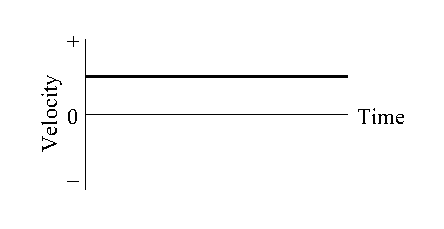
\includegraphics[width=0.45\textwidth]{velocity/velocity_fig8.eps} \par}
%\answerspace{0.3cm}
\begin{lab_axis}[lab_noticks_2quads,
	height = {2.0in}, width = {2.5in},
	xlabel={Time},
	ylabel={Velocity},
	plus_minus_zero_labels,
	]
\addplot[domain=0:0.9] {0.5};
\end{lab_axis}
\answerspace{0.2in}

2. How do you move to create a straight-line velocity-time graph that slopes
up from zero, as shown below?

%\vspace{0.3cm}
%{\par\raggedright 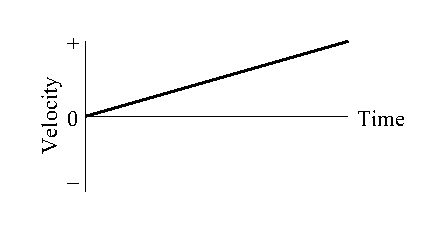
\includegraphics[width=0.45\textwidth]{velocity/velocity_fig9.eps} \par}
%\answerspace{0.3cm}
\begin{lab_axis}[lab_noticks_2quads,
	height = {2.0in}, width = {2.5in},
	xlabel={Time},
	ylabel={Velocity},
	plus_minus_zero_labels,
	]
\addplot[domain=0:0.9] {x};
\end{lab_axis}
\answerspace{0.2in}

3. How do you move to create a straight-line velocity-time graph that slopes
down, as shown below?

%\vspace{0.3cm}
%{\par\raggedright 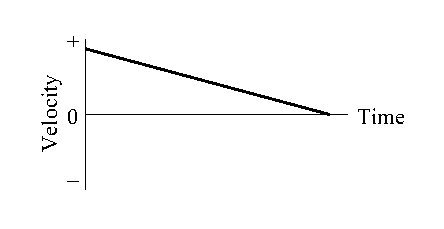
\includegraphics[width=0.45\textwidth]{velocity/velocity_fig10.eps} \par}
%\answerspace{0.3cm}
\begin{lab_axis}[lab_noticks_2quads,
	height = {2.0in}, width = {2.5in},
	xlabel={Time},
	ylabel={Velocity},
	plus_minus_zero_labels,
	]
\addplot[domain=0:0.9] {0.9 - x};
\end{lab_axis}
\answerspace{0.2in}

4. How do you move to make a horizontal line in the negative part of a velocity-time
graph, as shown below?

%\vspace{0.3cm}
%{\par\raggedright 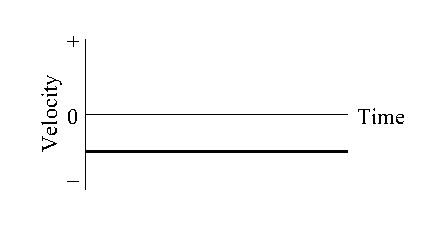
\includegraphics[width=0.45\textwidth]{velocity/velocity_fig11.eps} \par}
%\answerspace{0.3cm}
\begin{lab_axis}[lab_noticks_2quads,
	height = {2.0in}, width = {2.5in},
	xlabel={Time},
	ylabel={Velocity},
	plus_minus_zero_labels,
	]
\addplot[domain=0:0.9] {-0.5};
\end{lab_axis}
\answerspace{0.2in}

\pagebreak[4]
5. The velocity-time graph of an object is shown below. Figure out the total
change in position (displacement) of the object. Show your work.

Displacement = \_\_\_\_\_\_\_\_\_\_\_\_ meters.

\bigskip

%\vspace{0.3cm}
%{\par\raggedright 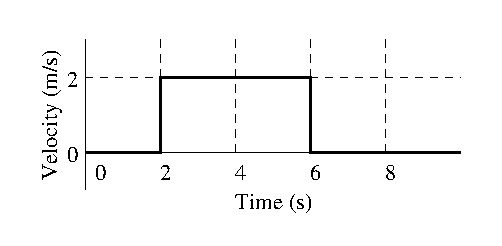
\includegraphics[width=0.55\textwidth]{velocity/velocity_fig12.eps} \par}
%\answerspace{0.6cm}
\begin{lab_axis}[lab_grid,
	height = {1.8in}, width = {3.5in},
	xlabel={Time (s)},
	ylabel={Velocity (m/s)},
	xmin=0, xmax=9,
	ymin=-1, ymax=3,
	xtick distance = 2,
	ytick distance = 2,
%	minor y tick num=1,
	y0_line,
	]
\addplot coordinates {(0,0) (2,0) (2,2) (6,2) (6,0) (10,0) };
\end{lab_axis}
\answerspace{0.1in}

6. The velocity graph below shows the motion of two objects, A and B. Answer
the following questions separately. Explain your answers when necessary. (a)
Is one faster than the other? If so,which one is faster? (A or B) (b) What does
the intersection mean? (c) Can one tell which object is ``ahead''?
(define ``ahead'') (d) Does either object A or B reverse direction?
Explain.

%\vspace{0.3cm}
%{\par\raggedright 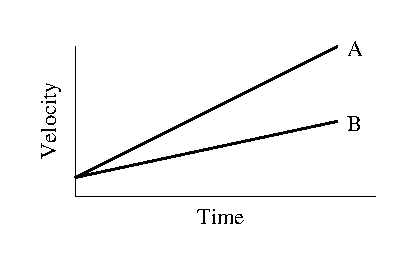
\includegraphics[width=0.45\textwidth]{velocity/velocity_fig13.eps} \par}
%\answerspace{0.6cm}
\begin{lab_axis}[lab_noticks_1quad,
	height = {1.8in}, width = {3.0in},
	xlabel={Time},
	ylabel={Velocity},
	]
\addplot coordinates {(0, 0.2) (0.9, 0.9)} node[right] {A};
\addplot coordinates {(0, 0.2) (0.9, 0.4)} node[right] {B};
\end{lab_axis}
\answerspace{0.7in}

7. The velocity graph below shows the motion of two objects, A and B. Answer
the following questions separately. Explain your answers when necessary. (a)
Is one faster than the other? If so,which one is faster? (A or B) (b) What does
the intersection mean? (c) Can one tell which object is ``ahead''?
(define ``ahead'') (d) Does either object A or B reverse direction?
Explain.

%\vspace{0.3cm}
%{\par\raggedright 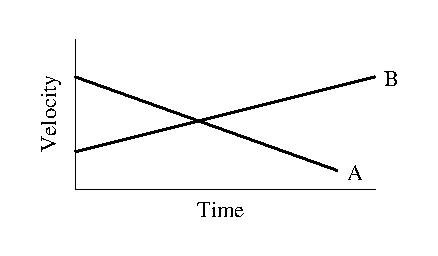
\includegraphics[width=0.45\textwidth]{velocity/velocity_fig14.eps} \par}
%\answerspace{0.6cm}
\begin{lab_axis}[lab_noticks_1quad,
	height = {1.8in}, width = {3.0in},
	xlabel={Time},
	ylabel={Velocity},
	]
\addplot coordinates {(0, 0.9) (0.7, 0.1)} node[right] {A};
\addplot coordinates {(0, 0.3) (0.9, 0.6)} node[right] {B};
\end{lab_axis}
\answerspace{0.7in}

\pagebreak[3]
Sketch the velocity-time graph corresponding to each of the following descriptions
of the motion of an object.

8. The object is moving away from the origin at a constant velocity.

%\vspace{0.3cm}
%{\par\centering 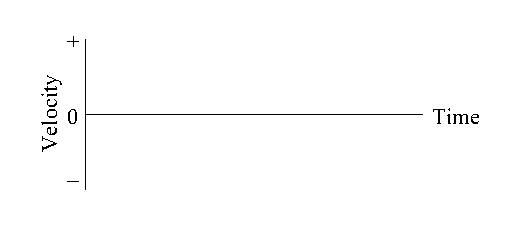
\includegraphics{velocity/velocity_fig15.eps} \par}
%\vspace{0.3cm}
\begin{lab_axis}*[lab_noticks_2quads,
	height = {1.8in}, width = {3.0in},
	xlabel={Time},
	ylabel={Velocity},
	plus_minus_zero_labels,
	]
\end{lab_axis}

9. The object is standing still.

%\vspace{0.3cm}
%{\par\centering 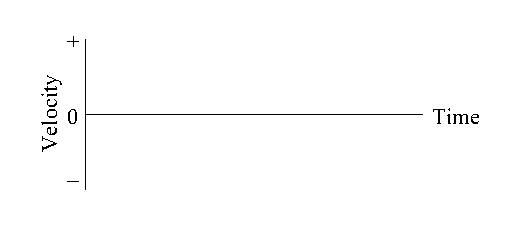
\includegraphics{velocity/velocity_fig15.eps} \par}
%\vspace{0.3cm}
\begin{lab_axis}*[lab_noticks_2quads,
	height = {1.8in}, width = {3.0in},
	xlabel={Time},
	ylabel={Velocity},
	plus_minus_zero_labels,
	]
\end{lab_axis}

10. The object moves toward the origin at a steady (constant) velocity for 10
s and then stands still for 10 s.

%\vspace{0.3cm}
%{\par\centering 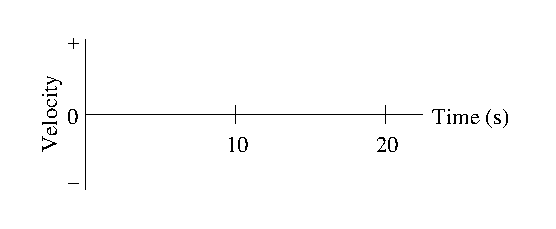
\includegraphics{velocity/velocity_fig16.eps} \par}
%\vspace{0.3cm}
\begin{lab_axis}*[lab_noticks_2quads,
	height = {1.8in}, width = {3.0in},
	xlabel={Time (s)},
	ylabel={Velocity},
	xmax=23,
	xtick={10,20},
	plus_minus_zero_labels,
	]
\end{lab_axis}


11. The object moves away from the origin at a steady (constant) velocity for
10 s, reverses direction and moves back toward the origin at the same speed
for 10 s.

%\vspace{0.3cm}
%{\par\centering 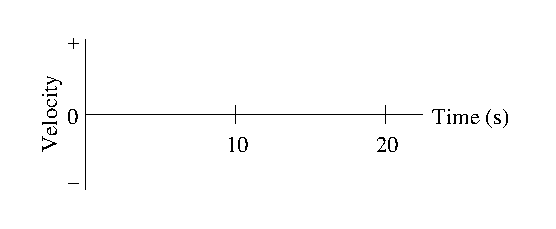
\includegraphics{velocity/velocity_fig16.eps} \par}
%\vspace{0.3cm}
\begin{lab_axis}*[lab_noticks_2quads,
	height = {1.8in}, width = {3.0in},
	xlabel={Time (s)},
	ylabel={Velocity},
	xmax=23,
	xtick={10,20},
	plus_minus_zero_labels,
	]
\end{lab_axis}





\section{Relating Position and Velocity Graphs\footnote{
1990-93 Dept. of Physics and Astronomy, Dickinson College. Supported by FIPSE
(U.S. Dept. of Ed.) and NSF. Portions of this material may have been modified
locally and may not have been classroom tested at Dickinson College.
}}

\makelabheader %(Space for student name, etc., defined in master.tex or labmanual_formatting_commands.tex)

\medskip
\textbf{Objective }

To understand the relationship between position \textit{vs.}~time and velocity \textit{vs.}~time
graphs.

\medskip

\textbf{Apparatus} 

\begin{itemize}[nosep]
\item Pasco 550 Interface
\item Ultrasonic motion detector 
\item \textit{Capstone} software (\filename{P\_V\_Graphs.cap} experiment file)
\item Wooden board
\end{itemize}

\medskip
\textbf{Introduction} 

You have looked at position and velocity \textit{vs.}~time graphs separately. Since position
vs. time and velocity \textit{vs.}~time graphs are different ways to represent the same
motion, it ought to be possible to figure out the velocity at which someone
is moving by examining her/his position \textit{vs.}~time graph. Conversely, you ought
to be able to figure out how far someone has traveled (change in position) from
a velocity \textit{vs.}~time graph.


\medskip

\textbf{Activity 1: Predicting Velocity Graphs from Position Graphs} 

Open the file \filename{P\_V\_Graphs.cap} in the \filename{\coursefolder} folder.
For some of the runs it may be necessary to adjust the time axis for one of the graphs so that the time scales are the same for the position and velocity graphs.

(a) Carefully study the position graph shown below and predict the velocity
vs. time graph that would result from the motion. Using a dashed line, sketch
your prediction of the corresponding velocity \textit{vs.}~time graph on the velocity
axes.

%\vspace{0.3cm}
%{\par\centering 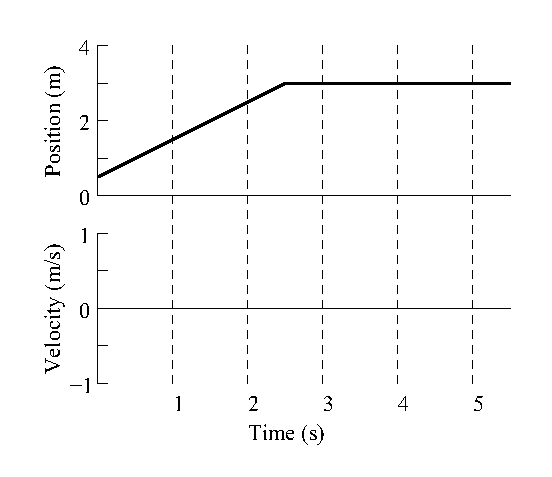
\includegraphics{relating/relating_fig1.eps} \par}
%\vspace{0.3cm}
\begin{lab_groupplot}*{\makegroupverticals[2]{2.5}{0}{5}}
					[lab_grid,
	group style={
		group size=1 by 2,
		xlabels at=edge bottom,
%		xticklabels at=edge bottom,
		vertical sep=0.4in
		},
	width=4in,
	height=2in,
	xlabel=Time (s),
	xmin=0, xmax=5,
	minor x tick num=1,
	]
\nextgroupplot[
	ymin=0,ymax=4, 
	ylabel={Position (m)},
	ylabel_align={-1},
	]
\addplot coordinates{(0,0.5) (2.5,3) (5,3)};

\nextgroupplot[
	ymin=-1,ymax=1, 
	ytick distance = 1, 
	minor y tick num=1, 
	y0_line,
	ylabel={Velocity (m/s)},
	]
\end{lab_groupplot}


(b) After each person in your group has sketched a prediction, test your prediction
by matching the position \textit{vs.}~time graph shown. When you have made a good duplicate
of the position graph, sketch your actual graph over the existing position vs. time graph.
Use a solid line to draw the actual velocity graph on the same graph with
your prediction. (Do not erase your prediction).

(c) How would the position graph be different if you moved faster? Slower? 
\answerspace{15mm}

(d) How would the velocity graph be different if you moved faster? Slower? 
\answerspace{15mm}

\textbf{Activity 2: Average Velocity Calculations} 

(a) Find your average velocity \emph{during the time you were moving at constant speed} from your velocity graph in the previous activity. To do this, use the \textbf{Statistics} function on the graph menu bar to determine the average velocity and the standard deviation on the \emph{left} part of the graph (where the velocity is approximately constant). See \textbf{Appendix \ref{capstone}: Capstone} for instructions on how to do this.

%Velocity values (m/s) \rule{0.5in}{0.1pt} \rule{0.5in}{0.1pt} \rule{0.5in}{0.1pt} \rule{0.5in}{0.1pt} \rule{0.5in}{0.1pt} \rule{0.5in}{0.1pt} \rule{0.5in}{0.1pt} \rule{0.5in}{0.1pt} \rule{0.5in}{0.1pt} \rule{0.5in}{0.1pt}
\answerspace{5mm}

Average value of the velocity: \rule{1.0in}{0.1pt} m/s

Standard deviation: \rule{1.0in}{0.1pt} m/s     (This can be taken as an uncertainty.)

Average velocity with uncertainty: \rule{1.5in}{0.1pt} m/s

(b) Average velocity during a particular time interval can also be calculated
as the change in position divided by the change in time. (The change in position
is often called the displacement.) By definition, this is also the slope of
the position \textit{vs.}~time graph for that time period. Select the position vs. time graph and open the \textbf{Delta Tool} function on the graph menu bar.  Set the cursor on one point on the position graph, right click on this point and select Show Delta Tool.  There will then be two cursors.  Set one cursor on one point on the position graph and the other on another point on the graph.  The changes in position and time will then be shown on the graph. (For a more accurate answer, use two points as far apart
as possible but still typical of the motion, \emph{and within the time 
interval over which you took velocity readings in part (a)}.) 
Record the values of \( \Delta x\) and \( \Delta t\) here:
\answerspace{10mm}

(c) Divide the change in position by the change in time to calculate the average velocity.  Show your calculation here:
\answerspace{15mm}

(d) Is the average velocity positive or negative? Is this what you expected? 
\answerspace{15mm}

\pagebreak[2]
(e) Does the average velocity you just calculated from the position graph fall within the range of values determined in part (a) from the velocity graph? Would you expect them to agree? How would you account for any differences?
\vspace{20mm}

\textbf{Activity 3: Finding Position from a Velocity Graph }

(a) Carefully study the velocity graph that follows. Using a dashed line, sketch your prediction of the corresponding position graph on the top set of axes.
(Assume that you started at the 1-meter mark.)

%\vspace{0.3cm}
%{\par\centering 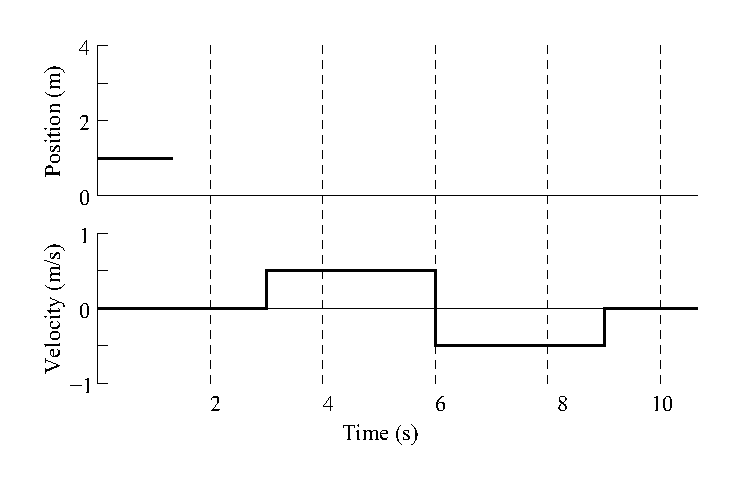
\includegraphics{relating/relating_fig2.eps} \par}
%\answerspace{0.3cm}
\begin{lab_groupplot}*{\makegroupverticals[2]{3,6,9}{0}{11}}
					[lab_grid,
	group style={
		group size=1 by 2,
		xlabels at=edge bottom,
%		xticklabels at=edge bottom,
		vertical sep=0.5in
		},
	width=5in,
	height=2in,
	xlabel=Time (s),
	xmin=0, xmax=11,
	xtick distance = 2,
	minor x tick num=1,
	minor y tick num=1,
	]
\nextgroupplot[
	ymin=0,ymax=4, 
	ytick distance = 2,
	ylabel={Position (m)},
	ylabel_align={-1},
	]
\addplot coordinates{(0,1) (1.5,1)};

\nextgroupplot[
	ymin=-1,ymax=1, 
	ytick distance = 1, 
	minor y tick num=1, 
	ylabel={Velocity (m/s)},
	y0_line,
	]
\addplot coordinates{(0,0) (3,0) (3,0.5) (6,0.5) (6,-0.5) (9,-0.5) (9,0) (11,0)};
\end{lab_groupplot}

(b) After each person has sketched a prediction, do your group's best to duplicate the bottom (velocity \textit{vs.}~time) graph by walking. When you have made a good duplicate of the velocity \textit{vs.}~time graph, draw your actual result over the existing velocity \textit{vs.}~time graph. Use a solid line on the top graph to draw the actual position vs. time graph on the same axes with your prediction. Do not erase your prediction.

(c) How can you tell from a velocity \textit{vs.}~time graph that the moving object has
changed direction?
\answerspace{10mm}

(d) What is the velocity at the moment the direction changes? 
\answerspace{10mm}

(e) Is it possible to actually move your body (or an object) to make vertical
lines on a position \textit{vs.}~time graph? Why or why not? What would the velocity
be for a vertical section of a position \textit{vs.}~time graph? 
\answerspace{10mm}

\pagebreak[2]
(f) How can you tell from a position \textit{vs.}~time graph that your motion is steady
(motion at a constant velocity)? 
\answerspace{10mm}

(g) How can you tell from a velocity \textit{vs.}~time graph that your motion is steady
(constant velocity)? 
\answerspace{20mm}

\textbf{Homework} 

1. Draw the velocity graphs for an object whose motion produced the position-time
graphs shown below on the left.  Note: Unlike most real objects, you can assume these objects can
change velocity so quickly that it looks instantaneous with this time scale.

\begin{center}
\begin{lab_axis}[lab_grid,
	height=1.6in, width=2in,
	xmin=0,xmax=5,
	xlabel={Time (s)},
	ymin=0,ymax=4,
	ylabel={Position (m)},
	xtick distance=1,	 ytick distance=1,
	]
\addplot coordinates{(0,0) (4,4)};
\end{lab_axis}
\hspace{0.3in}
\begin{lab_axis}[lab_grid,
	height=1.6in, width=2in,
	xmin=0,xmax=5,
	xlabel={Time (s)},
	ymin=-2,ymax=2,
	ylabel={Velocity (m/s)},
	xtick distance=1,	 ytick distance=1,
	]
\end{lab_axis}
\end{center}

\begin{center}
\begin{lab_axis}[lab_grid,
	height=1.6in, width=2in,
	xmin=0,xmax=5,
	xlabel={Time (s)},
	ymin=0,ymax=4,
	ylabel={Position (m)},
	xtick distance=1,	 ytick distance=1,
	]
\addplot coordinates{(0,0) (1,2) (5,4)};
\end{lab_axis}
\hspace{0.3in}
\begin{lab_axis}[lab_grid,
	height=1.6in, width=2in,
	xmin=0,xmax=5,
	xlabel={Time (s)},
	ymin=-2,ymax=2,
	ylabel={Velocity (m/s)},
	xtick distance=1,	 ytick distance=1,
	]
\end{lab_axis}
\end{center}

\begin{center}
\begin{lab_axis}[lab_grid,
	height=1.6in, width=2in,
	xmin=0,xmax=5,
	xlabel={Time (s)},
	ymin=0,ymax=4,
	ylabel={Position (m)},
	xtick distance=1,	 ytick distance=1,
	]
\addplot coordinates{(0,0) (2,2) (5,1)};
\end{lab_axis}
\hspace{0.3in}
\begin{lab_axis}[lab_grid,
	height=1.6in, width=2in,
	xmin=0,xmax=5,
	xlabel={Time (s)},
	ymin=-2,ymax=2,
	ylabel={Velocity (m/s)},
	xtick distance=1,	 ytick distance=1,
	]
\end{lab_axis}
\end{center}

%\vspace{0.3cm}
%{\par\centering 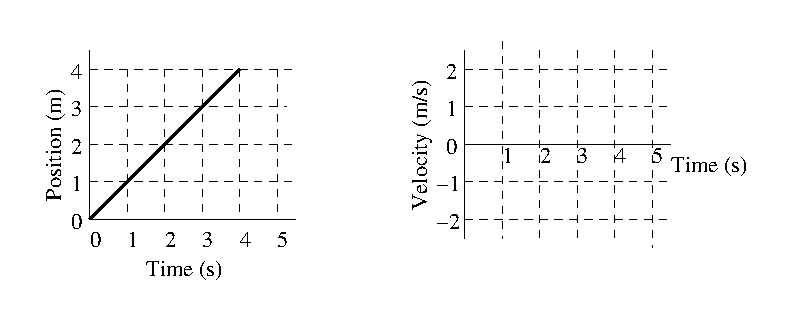
\includegraphics{relating/relating_fig3.eps} \par}
%\vspace{0.3cm}
%
%\vspace{0.3cm}
%{\par\centering 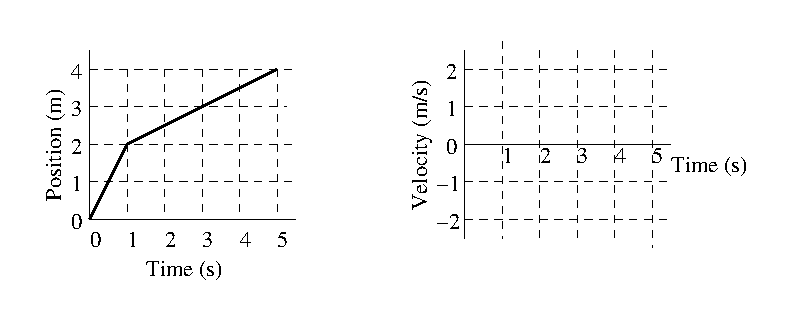
\includegraphics{relating/relating_fig4.eps} \par}
%\vspace{0.3cm}
%
%\vspace{0.3cm}
%{\par\centering 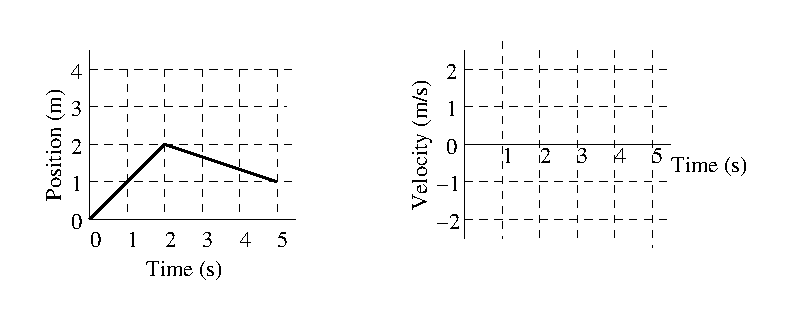
\includegraphics{relating/relating_fig5.eps} \par}
%\vspace{0.3cm}

\pagebreak[3]
2. Draw careful graphs below of position and velocity for a cart that (a) moves
away from the origin at a slow and steady (constant) velocity for the first
5 seconds; (b) moves away at a medium-fast, steady (constant) velocity for the
next 5 seconds; (c) stands still for the next 5 seconds; (d) moves toward the
origin at a slow and steady (constant) velocity for the next 5 seconds; (e)
stands still for the last 5 seconds.

%\vspace{0.3cm}
%{\par\centering 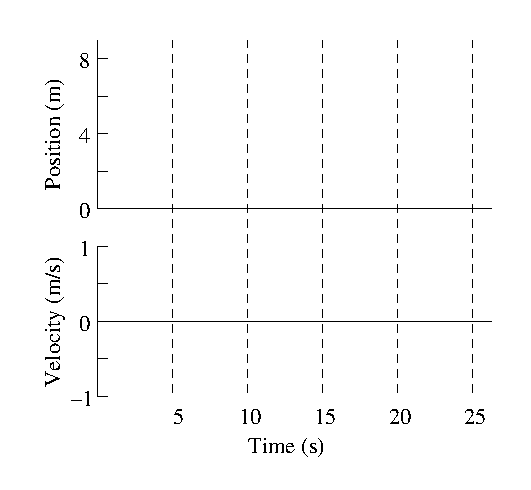
\includegraphics{relating/relating_fig6.eps} \par}
%\vspace{0.3cm}
\begin{lab_groupplot}*{}
					[lab_grid,
	group style={
		group size=1 by 2,
		xlabels at=edge bottom,
%		xticklabels at=edge bottom,
		vertical sep=0.3in,
		},
	width=4in,
	height=2in,
	xlabel=Time (s),
	xmin=0, xmax=25,
	minor x tick num=1
	]
\nextgroupplot[
	ymin=0,ymax=8, 
	ylabel={Position (m)},
	ylabel_align={-1},
	]
\nextgroupplot[
	ymin=-1,ymax=1, 
	ytick distance = 1, 
	minor y tick num=1, 
	y0_line,
	ylabel={Velocity (m/s)},
	]
\end{lab_groupplot}



%\section{Instantaneous Velocity}

\makelabheader %(Space for student name, etc., defined in master.tex or labmanual_formatting_commands.tex)

{\noindent \bf Objectives:} 

\begin{itemize}[nosep]
\item To make plausible the idea of velocity at an instant. 
\item To demonstrate that nonuniform motion appears increasingly uniform as the time interval becomes successively shorter. 
\item To understand the notion of ``taking a limit.''
\end{itemize}

\textbf{Apparatus:}

\begin{itemize}
\item Track and cart 
\item Pasco 550 Interface
\item Capstone software (\filename{P\_Graphs.cap} experiment file) %note reference to ``zoom in button''--- need to update?
\item Motion detector
\item Lab stand
\end{itemize}
{\noindent \bf Activity 1: An experiment} \begin{enumerate}

\item Open the file \filename{P\_Graphs.cap} in the \filename{\coursefolder} folder.
%Instantaneous Velocity application (under
%\textbf{Start} $\rightarrow$
%\textbf{Programs} $\rightarrow$ \textbf{131 Workshop}).

\item You will release a cart to roll down the track toward the motion
detector. \emph{Stop the cart before it hits the motion detector}. Also, be sure
that you aim the motion detector at the cart and that there are no people or
extraneous objects within a 20 degree cone of the track (with vertex
at the motion detector). Spurious motions within the sensitivity of
the motion detector give false signals.

\item Place the cart near the 2-meter mark at the raised end of the track, opposite that on which the motion detector is mounted.

\item Release the cart from rest and start recording data.

\item A graph with dots at regular \textit{time} intervals will be created on the screen. Stop the cart before it hits the motion detector. You may need to repeat the data taking until you get a reasonable looking chart (see Question 1).

\item Print out a copy of the graph for each member of the lab group.

\end{enumerate}

\medskip

{\noindent \bf Questions:}

1. Describe the distribution of the dots. Are they as you would have expected?
Is the motion it represents uniform or not? Explain. 
\answerspace{20mm}

\pagebreak[2]
2. Using the cursor, select ten data points on your graph. Click on the Zoom
In button on the graph menu bar until the highlighted data points span the graph.
Notice that the Zoom In button has the effect of viewing the data over successively
shorter time intervals. What does examining the data over successively shorter
time intervals demonstrate? Explain.
\answerspace{20mm}

3. Use the Smart Tool on the graph menu bar to record the position and time
for the first and last points highlighted on the graph. Calculate \( \Delta x/\Delta t \)
and explain the significance of this quantity.
\answerspace{20mm}

{\noindent \bf Discussion} You just approximated the instantaneous velocity for the central point of your section of dots. The instantaneous velocity is the velocity the object would have at a particular instant if it were moving at uniform velocity during the entire interval. You also approximated a derivative: the ratio of the displacement to the time interval as the time interval approaches zero seconds. 

{\noindent \bf Activity 2: A Graphing Exercise} \begin{enumerate}

\item On the next page, you will find three position versus clock reading graphs. The first one depicts motion over an eight second time interval. We want to know the instantaneous velocity at clock reading 3 sec.

\item On the second graph, replot the outlined segment of the first graph, this time magnifying both position and time by a factor of ten.

\item On the third graph, magnify again by a factor of ten the equivalent section of the second graph around clock reading 3 sec and position 16 cm. 

\item If you are satisfied with the straightness of the line in the third graph, calculate $\frac{\Delta s}{\Delta t}$, the average velocity for this interval. Since the line is sufficiently straight, the result of your calculation may be identified also as the instantaneous velocity at the midpoint of the interval.

\item The curve in the first graph depicts the motion of the object. Determine the equation of motion (the equation of the curve).

\item Take the derivative of this equation of motion and evaluate it at the central clock reading of your final interval. This is also a determination of the instantaneous velocity at that clock reading.

\end{enumerate}

\medskip

{\noindent \bf Questions:}

1. Compare your two calculations of the instantaneous velocity. Are they the
same or do they differ? Should they be the same or different? Explain. 
\answerspace{20mm}

2. Plot a line on the first graph through the point (3~s, 16~cm) which has the
slope of the line in the last graph. What is this line in relation to the motion
curve?
\answerspace{20mm}

\pagebreak[2]
\vspace{0.3cm}
{\par\centering 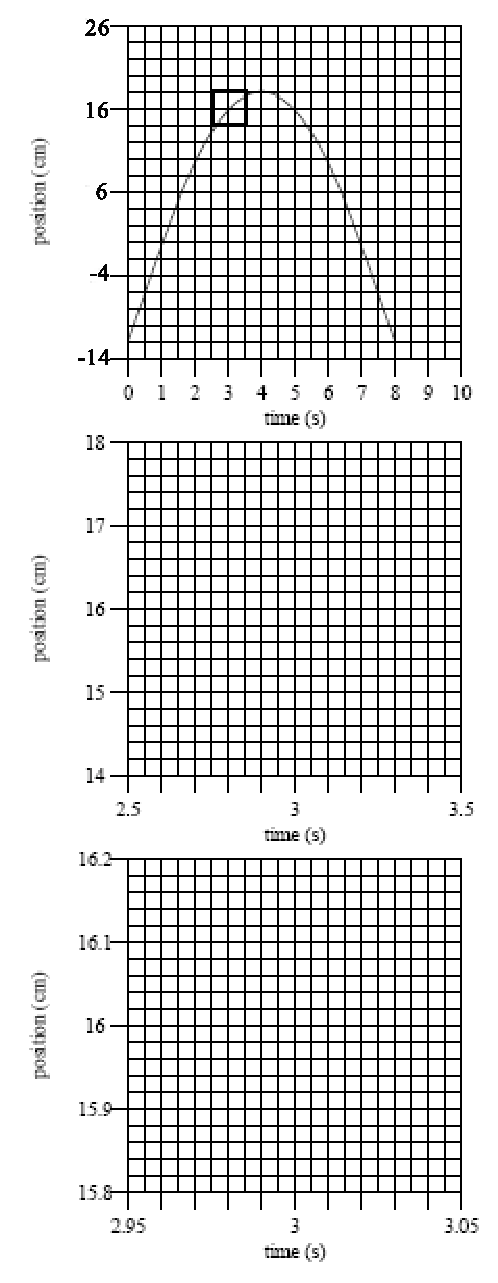
\includegraphics{instantaneous_velocity/instantaneous_velocity_fig1.eps} \par}
\vspace{0.3cm}



\section{Changing Motion\footnote{
1990-93 Dept. of Physics and Astronomy, Dickinson College. Supported by FIPSE
(U.S. Dept. of Ed.) and NSF. Portions of this material may have been modified
locally and may not have been classroom tested at Dickinson College.
}}
\label{changing_motion}

\makelabheader %(Space for student name, etc., defined in master.tex or labmanual_formatting_commands.tex)

\bigskip
\textbf{Objectives} 
\vspace{-\parskip}
\begin{itemize}
\item To learn how to relate graphs of acceleration \textit{vs.}~time to the motions they represent. 
\item To understand the relationship between position \textit{vs.}~time, velocity \textit{vs.}~time,
and acceleration \textit{vs.}~time graphs.
\end{itemize}

\textbf{Introduction: Velocity and Acceleration Graphs} 

We are interested in having you learn to describe simple motions in which the
velocity of an object is changing. In order to learn to describe motion in more
detail for some simple situations, you will be asked to observe and describe
the motion of a dynamics cart on a track. Although graphs and words are still
important representations of these motions, you will also be asked to draw velocity
vectors, arrows that indicate both the direction and speed of a moving object.
Thus, you will also learn how to represent simple motions with velocity diagrams.

In the last session, you looked at position \textit{vs.}~time and velocity \textit{vs.}~time graphs
of the motion of your body as you moved at a ``constant'' velocity.
The data for the graphs were collected using a motion detector. Your goal in
this session is to learn how to describe various kinds of motion in more detail.
It is not enough when studying motion in physics to simply say that ``the
object is moving toward the right'' or ``it is standing still.''
You have probably realized that a velocity \textit{vs.}~time graph is better than a position
vs. time graph when you want to know how fast and in what direction you are
moving at each instant in time as you walk. When the velocity of an object is
changing, it is also important to know how it is changing. The rate of change
of velocity is known as the acceleration. 

In order to get a feeling for acceleration, it is helpful to create and learn
to interpret velocity \textit{vs.}~time and acceleration \textit{vs.}~time graphs for some relatively
simple motions of a cart on a track. You will be observing the cart with the
motion detector as it moves at a constant velocity and as it changes its velocity
at a constant rate. Use the 
\filename{P\_V\_A\_Graphs.cap} program in the \filename{\coursefolder} folder
for all of the activities in this unit.

\bigskip
\textbf{Apparatus} 
\vspace{-\parskip}
\begin{itemize}
\item Pasco 550 Interface
\item Ultrasonic motion detector 
\item \textit{Capstone} software (\filename{P\_V\_A\_Graphs.cap} experiment file)
\item Collision cart and track 
\item Lab stand to incline the track 
\end{itemize}

\textbf{Activity 1: Graphs of Constant Velocity} 

Let's start by giving the cart a push along the level track and graphing its
motion. 

(a) Based on your observations of the motions of your body in the last session,
how should the position and velocity graphs look if you move the cart at a constant
velocity away from the motion detector starting at the 0.5 meter mark? Sketch
your predictions with dashed lines on the axes that follow.

%\vspace{-0.1in}
%{\par\centering 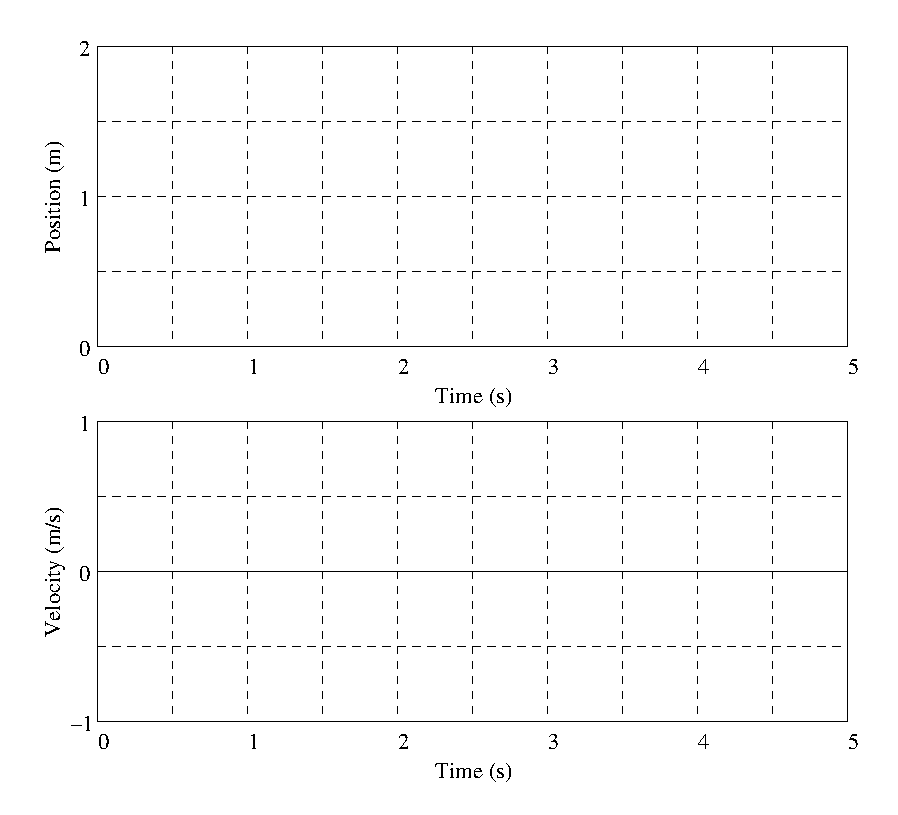
\includegraphics[scale=1]{changing/changing_fig1.eps} \par}
%\vspace{-0.1in}

\begin{lab_groupplot}*{}
					[lab_grid,
	group style={
		group size=1 by 2,
		xlabels at=edge bottom,
		vertical sep=0.4in,
		},
	scale only axis=true,
	width=5in,  %by setting only the width, it automatically preserves default aspect ratio of 1:1
	xlabel=Time (s),
	xmin=0, xmax=5,
	xtick distance = 1, 
	ytick distance = 1, 
	minor tick num=1
	]
\nextgroupplot[
	ymin=0,ymax=2, 
	ylabel={Position (m)},
	ylabel_align={-1},
	]
\nextgroupplot[
	ymin=-1,ymax=1, 
	y0_line,
	ylabel={Velocity (m/s)},
	]
\end{lab_groupplot}

(b) Acceleration is defined as the time rate of change of velocity. Sketch your
prediction of the cart acceleration on the axes that follow using a dashed line.

\begin{lab_axis}*[lab_grid,
	scale only axis=true,
	width=5in,
	xlabel={Time (s)},
	xmin=0, xmax=5,
	ymin=-1,ymax=1, 
	xtick distance = 1, 
	ytick distance = 1, 
	minor tick num=1,
	y0_line,
	ylabel={Acceleration (m/s$^2$)},
	]
\end{lab_axis}

%\vspace{-0.1in}
%{\par\centering \includegraphics[scale=1]{changing/changing_fig2.eps} \par}
%\vspace{-0.1in}


(c) Test your prediction. Be sure that the cart is never closer than 0.15 meter
from the motion detector. Try several times until you get a fairly constant
velocity. Sketch your results with solid lines on the axes shown above. The
acceleration \textit{vs.}~time graphs will exhibit small fluctuations due to irregularities
in the motion of the cart. You should ignore these fluctuations and draw smooth
patterns.

\pagebreak[2]
(d) Did your graphs agree with your predictions? What characterizes constant
velocity motion on a position \textit{vs.}~time graph? 
\answerspace{10mm}

(e) What characterizes constant velocity motion on a velocity \textit{vs.}~time graph?
\answerspace{10mm}

(f) What characterizes constant velocity motion on an acceleration \textit{vs.}~time graph?
\answerspace{10mm}

%\textbf{Finding Accelerations} 
\textbf{Activity 2: Representing Acceleration} 

To find the average acceleration of the cart during some time interval (the
average time rate of change of its velocity), you must measure its velocity
at two different times, calculate the difference between the final value and
the initial value and divide by the time interval.

To find the acceleration vector from two velocity vectors, you must first find
the vector representing the change in velocity by subtracting the initial velocity
vector from the final one. Then you divide this vector by the time interval. 


(a) Calculate the average acceleration during some time interval from your velocity graph in Activity 1.  Does the result agree with your acceleration graph in Activity 1?
\answerspace{20mm}

(b) The diagram below shows the positions of the cart at equal time intervals.
(This is like taking snapshots of the cart at equal time intervals.) At each
indicated time, sketch, and label, a vector above the cart which might represent the velocity
of the cart at that time while it is moving at a constant velocity away from
the motion detector.

%\vspace{0.3cm}
%{\par\centering \includegraphics{changing/changing_fig3.eps} \par}
{\par\centering \includegraphics{changing/carts_const_v.eps} \par}
%\vspace{0.3cm}

(c) Show how you would find the vector representing the change in velocity
between the times 1.0 s and 2.0 s by creating a vector diagram using the 
vectors above. From the resultant vector, what value would you calculate for 
the acceleration? Is this value in agreement
with the acceleration graph you obtained in Activity 1?
\answerspace{20mm}

\pagebreak[2]
%\textbf{Speeding Up at a Moderate Rate} 
\textbf{Activity 3: Graphs Depicting Speeding Up} 

In this activity you will look at velocity and acceleration graphs of the
motion of a cart when its velocity is changing. You will be able to see how
these two representations of the motion are related to each other when the cart
is speeding up.

In order to get your cart speeding up smoothly \textit{use the lab stand to raise the
track several centimeters at the end where the motion detector is mounted}.

(a) Predict the shape of the position, velocity, and acceleration \textit{vs.}~time graphs
for the cart moving away from the sensor and speeding up. Sketch your predictions
on the following axes using dashed lines.

%\vspace{-0.2cm}
%{\par\centering \includegraphics[scale=0.93]{changing/changing_fig1.eps} \par}
%%\vspace{0.3cm}

%\vspace{-0.4cm}
%{\par\centering \includegraphics[scale=0.93,trim={0 0 0 0.4cm},clip]{changing/changing_fig2.eps} \par}
%%\vspace{0.3cm}

\begin{lab_groupplot}*{}
					[lab_grid,
	group style={
		group size=1 by 3,
		xlabels at=edge bottom,
		vertical sep=0.4in,
		},
	scale only axis=true,
	axis equal image,
	width=4.5in,  %by setting only the width, it automatically preserves aspect ratio of 1:1
	xlabel=Time (s),
	xmin=0, xmax=5,
	xtick distance = 1, 
	ytick distance = 1, 
	minor tick num=1
	]
\nextgroupplot[
	ymin=0,ymax=2, 
	ylabel={Position (m)},
	ylabel_align={-1},
	]
\nextgroupplot[
	ymin=-1,ymax=1, 
	y0_line,
	ylabel={Velocity (m/s)},
	]
\nextgroupplot[
	ymin=-1,ymax=1, 
	y0_line,
	ylabel={Acceleration (m/s$^2$)},
	]
\end{lab_groupplot}



(b) Create graphs of the motion of your cart as it moves away from the detector
and speeds up. Sketch the graphs neatly on the above axes using solid lines.

\pagebreak[2]
(c) How does your position graph differ from the position graphs for steady
(constant velocity) motion? 
\vspace{13mm}

(d) What feature of your velocity graph signifies that the motion was away from
the detector? 
\vspace{13mm}

(e) What feature of your velocity graph signifies that the cart was speeding
up? How would a graph of motion with a constant velocity differ? 
\vspace{13mm}

(f) During the time that the cart is speeding up, is the acceleration positive
or negative? How does speeding up while moving away from the detector result
in this sign of acceleration? Hint: Remember that acceleration is the rate of
change of velocity. Look at how the velocity is changing. 
\vspace{13mm}

(g) How does the velocity vary in time as the cart speeds up? Does it increase
at a steady rate or in some other way? 
\vspace{13mm}

(h) How does the acceleration vary in time as the cart speeds up? Is this what
you expect based on the velocity graph? Explain.
\vspace{13mm}

(i) Do not delete the graphs from the computer screen.  They will be used in Activity 5.
\vspace{10mm}

\textbf{Activity 4: Using Vectors to Describe Acceleration} 

Let's return to the Vector Diagram representation and use it to describe the
acceleration.

(a) The diagram that follows shows the positions of the cart at equal time intervals.
At each indicated time, sketch, and label, a vector above the cart which might represent
the velocity of the cart at that time while it is moving away from the motion
detector and speeding up.

\vspace{0.3cm}
%{\par\centering \includegraphics{changing/changing_fig4.eps} \par}
{\par\centering \includegraphics{changing/carts_const_a.eps} \par}
\vspace{0.3cm}

(b) Show below how you would find the approximate length and direction of the
vector representing the change in velocity between the times 1.0 s and 2.0 s
by creating a vector diagram using the vectors above. No quantitative 
calculations are needed. Based on the direction of the resultant vector and 
the direction of the positive x-axis, what is the sign of the acceleration? 
Does this agree with your answer to Activity 3 (f)?
\answerspace{20mm}

%\textbf{Measuring Acceleration }
\textbf{Activity 5: Measuring and Calculating Accelerations}

In this investigation you will analyze the motion of your accelerated cart quantitatively.
This analysis will be quantitative in the sense that your results will consist
of numbers. You will determine the cart's acceleration from the slope of your
velocity \textit{vs.}~time graph and compare it to the average acceleration read from
the acceleration \textit{vs.}~time graph. 

(a) Using the \textbf{Statistics} function on your acceleration graph from Activity 3, determine the average acceleration and the standard deviation by selecting only values from the portion of the graph after the cart was released and before you stopped it. See \textbf{Appendix \ref{capstone}: Capstone} for information on how to use the \textbf{Statistics} function. Record these values here:
\answerspace{20mm}

(b) Write the acceleration with its uncertainty (the standard deviation) here:
\answerspace{20mm}

(c) The average acceleration during a particular time period is defined as the
change in velocity divided by the change in time. This is the average rate of
change of velocity. By definition, the rate of change of a quantity graphed
with respect to time is also the slope of the curve. Thus the (average) slope
of an object's velocity \textit{vs.}~time graph is the (average) acceleration of the
object.

Select the velocity vs. time graph from Activity 3 and open the \textbf{Delta Tool} function on the graph menu bar. Determine quantities \( \Delta v\) and \( \Delta t\) for two points on the velocity graph using the Delta Tool, 
in the same way that you did on the position vs. time graph in the previous experiment. Record the values of 
\( \Delta v\) and \( \Delta t\) here:
\answerspace{20mm}

(d) Divide the change in velocity by the change in time. This is the average acceleration. Show your calculation here:
\answerspace{20mm}

\pagebreak[2]
(e) Is the acceleration positive or negative? Is this what you expected? 
\answerspace{15mm}

(f) Does the average acceleration you just calculated agree with the average
acceleration you calculated from the acceleration \textit{vs.}~time graph? Do you expect them to agree? How would you account for any differences? 
\answerspace{20mm}

\textbf{Activity 6: Speeding Up at a Faster Rate} 

(a) Suppose that you accelerate your cart at a faster rate by raising the end of the track several more centimeters. How would your velocity and acceleration graphs change? 
\answerspace{15mm}

(b) Resketch the velocity and acceleration graphs you found in Activity 3 using
the axes that follow.

%\vspace{-0.3cm}
%{\par\centering \includegraphics{changing/changing_fig5.eps} \par}
%\vspace{-0.3cm}

\begin{lab_groupplot}*{}
					[lab_grid,
	group style={
		group size=1 by 2,
		xlabels at=edge bottom,
		vertical sep=0.4in,
		},
	scale only axis=true,
	axis equal image,
	width=3.5in,  %by setting only the width, it automatically preserves aspect ratio of 1:1
	xlabel=Time (s),
	xmin=0, xmax=4,
	xtick distance = 1, 
	ytick distance = 1, 
	minor tick num=1
	]
\nextgroupplot[
	ymin=-1,ymax=1, 
	y0_line,
	ylabel={Velocity (m/s)},
	]
\nextgroupplot[
	ymin=-1,ymax=1, 
	y0_line,
	ylabel={Acceleration (m/s$^2$)},
	]
\end{lab_groupplot}

(c) In the previous set of axes, use a dashed line or another color to sketch
your predictions for the general graphs that depict a cart speeding up at a
faster rate. Exact predictions are not expected. We just want to know how you
think the general shapes of the graphs will change.

\pagebreak[2]
(d) Test your predictions by accelerating the cart with the end of the track raised several centimeters more than in Activity 3. Repeat if necessary to get nice graphs and then sketch the results using the axes that follow.

%%\vspace{0.3cm}
%{\par\centering \includegraphics{changing/changing_fig5.eps} \par}
%%\vspace{0.3cm}
\begin{lab_groupplot}*{}
					[lab_grid,
	group style={
		group size=1 by 2,
		xlabels at=edge bottom,
		vertical sep=0.4in,
		},
	scale only axis=true,
	axis equal image,
	width=3.5in,  %by setting only the width, it automatically preserves aspect ratio of 1:1
	xlabel=Time (s),
	xmin=0, xmax=4,
	xtick distance = 1, 
	ytick distance = 1, 
	minor tick num=1
	]
\nextgroupplot[
	ymin=-1,ymax=1, 
	y0_line,
	ylabel={Velocity (m/s)},
	]
\nextgroupplot[
	ymin=-1,ymax=1, 
	y0_line,
	ylabel={Acceleration (m/s$^2$)},
	]
\end{lab_groupplot}

(e) Did the general shapes of your velocity and acceleration graphs agree with
your predictions? How is the greater magnitude (size) of acceleration represented
on a velocity \textit{vs.}~time graph? 
\answerspace{25mm}

(f) How is the greater magnitude (size) of acceleration represented on an acceleration
vs. time graph? 
\answerspace{25mm}

\pagebreak[2]
\textbf{Homework} 

1. An object moving along a line (the + position axis) has the acceleration-time
graph shown below. Describe how the object might move to create this graph if
it is moving away from the origin.

%\vspace{0.3cm}
%{\par \centering \includegraphics{changing/changing_fig6.eps} \par}
\hspace{0.4in}
\begin{lab_axis}[lab_noticks_2quads,
	height = {1.8in}, width = {3.0in},
	xlabel={Time},
	ylabel={Acceleration},
	plus_minus_zero_labels,
	]
\addplot {0.5};
\end{lab_axis}
%\answerspace{1.5cm}

2. Sketch on the axes below a velocity-time graph that goes with the above acceleration-time
graph.

%\vspace{0.3cm}
%{\par\centering \includegraphics{changing/changing_fig7.eps} \par}
%\answerspace{1.0cm}
%\vspace{0.4cm}
\hspace{0.4in}
\begin{lab_axis}[lab_noticks_2quads,
	height = {1.8in}, width = {3.0in},
	xlabel={Time},
	ylabel={Velocity},
	plus_minus_zero_labels,
	]
\end{lab_axis}


3. For each of the velocity-time graphs below, sketch the shape of the acceleration-time
graph that goes with it.

\hspace{0.4in}
\begin{lab_groupplot}{}
					[lab_noticks_2quads,
	group style={
		group size=1 by 2,
		vertical sep=0.2in,
		},
	height = {1.8in}, width = {2.5in},
	xlabel=Time,
	plus_minus_zero_labels,
	]
\nextgroupplot[
	ylabel={Velocity},
	]
\addplot coordinates {(0, 0.0) (0.9, 0.8)};
\nextgroupplot[
	ylabel={Acceleration},
	]
\end{lab_groupplot}
\hspace{0.3in}
\begin{lab_groupplot}{\makegroupverticals[2]{0.3,0.6}{0}{1}}
					[lab_noticks_2quads,
	group style={
		group size=1 by 2,
		vertical sep=0.2in,
		},
	height = {1.8in}, width = {2.5in},
	xlabel=Time,
	plus_minus_zero_labels,
	]
\nextgroupplot[
	ylabel={Velocity},
	]
\addplot coordinates {(0, 0.0) (0.3, 0.0) (0.6,0.8) (0.9,0.8)};
\nextgroupplot[
	ylabel={Acceleration},
	]
\end{lab_groupplot}

%\vspace{0.3cm}
%{\par\centering \includegraphics{changing/changing_fig8.eps} \par}
%\vspace{0.3cm}

%\vspace{0.3cm}
%{\par\centering \includegraphics{changing/changing_fig9.eps} \par}
%\vspace{0.3cm}

4. The following is a velocity-time graph for a car.  What is the car's average acceleration? Show your work below.


%\vspace{0.3cm}
%{\par\centering \includegraphics{changing/changing_fig10.eps} \par}
%\vspace{0.3cm}
%
%\answerspace{30mm}
\hspace{0.4in}
\begin{lab_axis}[lab_grid,
	scale only axis=true,
	height = {1.5in}, width = {2.5in},
%	width=5in,
	xlabel={Time (s)},
	xmin=0, xmax=10,
	ymin=-4,ymax=4, 
%	xtick distance = 1, 
%	ytick distance = 1, 
%	minor tick num=1,
	y0_line,
	ylabel={Velocity (m/s)},
	]
\addplot coordinates {(0, 1.0) (10, 4)};
\end{lab_axis}

\pagebreak[3]
5. Which position-time graph below could be that for a cart that is steadily
accelerating away from the origin?

\begin{center}
\begin{lab_axis}[lab_noticks_1quad,
	height = {1.5in}, width = {2in},
	xlabel={Time},
	ylabel={Position},
	title={(a)},
	]
\addplot coordinates {(0, 0) (0.9,0.9)};
\end{lab_axis}
\hspace{0.3in}
\begin{lab_axis}[lab_noticks_1quad,
	height = {1.5in}, width = {2in},
	xlabel={Time},
	ylabel={Position},
	title={(b)},
	]
\addplot coordinates {(0, 0) (0.2,0.1) (0.7,0.8) (0.9,0.9)};
\end{lab_axis}
\hspace{0.3in}
\begin{lab_axis}[lab_noticks_1quad,
	height = {1.5in}, width = {2in},
	xlabel={Time},
	ylabel={Position},
	title={(c)},
	]
\addplot {x^2 };
\end{lab_axis}
\end{center}

%\vspace{0.3cm}
%{\par\centering \includegraphics{changing/changing_fig11.eps} \par}
%\vspace{0.3cm}

A car can move along a line (the + position axis). Sketch velocity-time and
acceleration-time graphs which correspond to each of the following descriptions
of the car's motion.

6. The car starts from rest and moves away from the origin increasing its speed
at a steady rate.

%\vspace{0.3cm}
%{\par\centering \includegraphics[width=0.55\textwidth]{changing/changing_fig12.eps} \par}
%\answerspace{0.3cm}
\hspace{0.4in}
\begin{lab_axis}[lab_noticks_2quads,
	height = {1.8in}, width = {2.5in},
	xlabel={Time},
	ylabel={Velocity},
	plus_minus_zero_labels,
	]
\end{lab_axis}
\hspace{0.2in}
\begin{lab_axis}[lab_noticks_2quads,
	height = {1.8in}, width = {2.5in},
	xlabel={Time},
	ylabel={Acceleration},
	plus_minus_zero_labels,
	]
\end{lab_axis}

7. The car is moving away from the origin at a constant velocity.

%\vspace{0.3cm}
%{\par\centering \includegraphics[width=0.55\textwidth]{changing/changing_fig12.eps} \par}
%\answerspace{0.3cm}

%\pagebreak[2]
%\newpage
\hspace{0.4in}
\begin{lab_axis}[lab_noticks_2quads,
	height = {1.8in}, width = {2.5in},
	xlabel={Time},
	ylabel={Velocity},
	plus_minus_zero_labels,
	]
\end{lab_axis}
\hspace{0.2in}
\begin{lab_axis}[lab_noticks_2quads,
	height = {1.8in}, width = {2.5in},
	xlabel={Time},
	ylabel={Acceleration},
	plus_minus_zero_labels,
	]
\end{lab_axis}

8. The car starts from rest and moves away from the origin increasing its speed
at a steady rate twice as large as in (6) above.

%\vspace{0.3cm}
%{\par\centering \includegraphics[width=0.55\textwidth]{changing/changing_fig12.eps} \par}
%\vspace{0.3cm}
\hspace{0.4in}
\begin{lab_axis}[lab_noticks_2quads,
	height = {1.8in}, width = {2.5in},
	xlabel={Time},
	ylabel={Velocity},
	plus_minus_zero_labels,
	]
\end{lab_axis}
\hspace{0.2in}
\begin{lab_axis}[lab_noticks_2quads,
	height = {1.8in}, width = {2.5in},
	xlabel={Time},
	ylabel={Acceleration},
	plus_minus_zero_labels,
	]
\end{lab_axis}

9. The car is moving away from the origin at a constant velocity twice as large
as in (7) above.

%\vspace{0.3cm}
%{\par\centering \includegraphics[width=0.55\textwidth]{changing/changing_fig12.eps} \par}
%\vspace{0.3cm}
\hspace{0.4in}
\begin{lab_axis}[lab_noticks_2quads,
	height = {1.8in}, width = {2.5in},
	xlabel={Time},
	ylabel={Velocity},
	plus_minus_zero_labels,
	]
\end{lab_axis}
\hspace{0.2in}
\begin{lab_axis}[lab_noticks_2quads,
	height = {1.8in}, width = {2.5in},
	xlabel={Time},
	ylabel={Acceleration},
	plus_minus_zero_labels,
	]
\end{lab_axis}




\section{Slowing Down, Speeding Up, and Turning\footnote{
1990-93 Dept. of Physics and Astronomy, Dickinson College. Supported by FIPSE
(U.S. Dept. of Ed.) and NSF. Portions of this material may have been modified
locally and may not have been classroom tested at Dickinson College.
}}

\makelabheader %(Space for student name, etc., defined in master.tex or labmanual_formatting_commands.tex)

\medskip
\textbf{Objectives }

\begin{itemize}
\item To learn how to relate graphs of acceleration \textit{vs.}~time to the motions they represent. 
\item To understand the relationship between velocity \textit{vs.}~time and acceleration vs.
time graphs.
\end{itemize}

\medskip
\textbf{About Slowing Down, Speeding Up and Turning }

In the previous session, you explored the characteristics of position \textit{vs.}~time,
velocity \textit{vs.}~time and acceleration  \textit{vs.}~time graphs of the motion of a dynamics
cart. In the cases examined, the cart was always moving away from a motion detector,
either at a constant velocity or with a constant acceleration. Under these conditions,
the velocity and acceleration are both positive. You also learned how to find
the magnitude of the acceleration from velocity \textit{vs.}~time and acceleration vs.
time graphs, and how to represent the velocity and acceleration using vectors. 

In the motions you studied in the last session, the velocity and acceleration
vectors representing the motion of the cart both pointed in the same direction.
In order to get a better feeling for acceleration, it will be helpful to examine
velocity \textit{vs.}~time and acceleration \textit{vs.}~time graphs for some slightly more complicated
motions of a cart on an inclined track. Again you will use the motion detector
to observe the cart as it changes its velocity at a constant rate. Only this
time the motion may be toward the detector, and the cart may be speeding up
or slowing down.

\medskip
\textbf{Apparatus }

\begin{itemize}
\item \textit{Science Workshop 750 Interface}
\item Ultrasonic motion detector 
\item \textit{Capstone} software (P, V \& A Graphs application)
\item Collision cart and track 
\item Lab stand to incline the track
\end{itemize}

\medskip
\textbf{Slowing Down and Speeding Up }

In this activity you will look at a cart moving along an inclined track and
slowing down. A car being brought to rest by the steady action of brakes is
a good example of this type of motion. Later you will examine the motion of
the cart toward the motion detector and speeding up. In both cases, we are interested
in the shapes of the velocity \textit{vs.}~time and acceleration \textit{vs.}~time graphs, as
well as the vectors representing velocity and acceleration. 

Let's start with the creation of velocity and acceleration graphs of when it
is moving away from the motion detector and slowing down. To do this activity,
the track should be inclined with a lab stand at one end and the motion detector set up at the \underline{lower end} of the track. Adjust the lab stand so that the track is raised a few centimeters at the opposite end from where the motion detector is located. Now when you give the cart a push away from the motion detector, it will slow down after it is released. In this activity you will examine the velocity and acceleration of this motion.

\pagebreak[2]
\textbf{Activity 1: Graphs Depicting Slowing Down} 

(a) If you give the cart a push away from the motion detector and release it,
will the acceleration be positive, negative or zero (after it is released)?
Sketch your predictions for the velocity \textit{vs.}~time and acceleration \textit{vs.}~time
graphs on the axes below using dashed lines.

\vspace{0.3cm}
{\par\centering \includegraphics{slowing/slowing_fig1.eps} \par}
\vspace{0.3cm}

(b) To test your predictions, open the \textbf{P, V \& A Graphs} application as you did in the previous experiment. Locate the cart 0.15 m from the motion detector and gently push the cart away from the motion detector once it starts clicking. Catch the cart \underline{before} it turns around or hits the end of the track.

Draw the results on the axes above using solid lines for the part of the motion
after the cart is released. You may have to try a few times to get a good run.  The acceleration \textit{vs.}~time graphs will exhibit small fluctuations due to irregularities in the motion of the cart. You should ignore these fluctuations and draw smooth patterns.

(c) Did the shapes of your velocity and acceleration graphs agree with your
predictions? How is the sign of the acceleration represented on a velocity vs.
time graph? 
\answerspace{15mm}

(d) How is the sign of the acceleration represented on an acceleration \textit{vs.}~time
graph? 
\answerspace{15mm}

\pagebreak[3]
(e) Is the sign of the acceleration what you predicted? How does slowing down
while moving away from the detector result in this sign of acceleration? Hint:
Remember that acceleration is the rate of change of velocity. Look at how the
velocity is changing.
\answerspace{20mm}

%\textbf{Constructing Acceleration Vectors for Slowing Down }
\textbf{Activity 2: Constructing Acceleration Vectors for Slowing Down}

Let's consider a diagrammatic representation of a cart which is slowing down
and use vector techniques to figure out the direction of the acceleration.

%\textbf{Activity 2: Vector Diagrams for Slowing Down} 

(a) The diagram that follows shows the positions of the cart at equal time intervals.
(This is like taking snapshots of the cart at equal time intervals.) At each
indicated time, sketch, and label, a vector above the cart which might represent the velocity
of the cart at that time while it is moving away from the motion detector and
slowing down.

\vspace{0.5cm}
%{\par\centering \includegraphics{slowing/slowing_fig2.eps} \par}
{\par\centering \includegraphics{slowing/carts_slowing.eps} \par}
\vspace{0.5cm}

(b) Show below how you would find the vector representing the change in velocity
between the times 1s and 2s by creating a vector diagram using the vectors 
 above. Based on the direction of the resultant vector and the direction of 
the positive x-axis, what is the sign of the acceleration? 
Does this agree with your answer to Question (e) in Activity 1?
\answerspace{25mm}

(c) By filling in the following table, state the general rules to predict the 
sign of the acceleration if you know the sign of the velocity (i.e., the 
direction of motion) and whether the object is speeding up or slowing down. 
Positive velocities have been investigated in this experiment and the previous 
one. Negative velocities we investigate below, so these are essentially 
predictions.

\vspace{0.3cm}
{\centering \begin{tabular}{|c|c|c|}
\hline
Velocity&
&
Acceleration\\
\hline
positive&
speeding up&
\\
\hline
positive&
slowing down&
\\
\hline
negative&
speeding up&
\\
\hline
negative&
slowing down&
\\
\hline
\end{tabular}\par}
\vspace{0.3cm}


%\newpage
\pagebreak[2]
\textbf{Activity 3: Speeding Up Toward the Motion Detector} 

Suppose the cart is allowed to speed up when traveling toward the motion 
detector. What will be the sign of the acceleration? Positive or negative? 

(a) Use the general rules that you stated in Activity 2 to predict the shapes
of the velocity and acceleration graphs. Sketch your predictions using dashed
lines on the axes that follow.

%\vspace{0.3cm}
{\par\centering \includegraphics{slowing/slowing_fig1.eps} \par}
%\vspace{0.3cm}

(b) Test your predictions by releasing the cart from rest at the raised end of the track after the motion detector starts clicking. Catch the cart before it gets too close to the detector.  
Draw the results using solid lines on the axes above. You may have to try a
few times to get a good run.

(c) How does your velocity graph show that the cart was moving toward the detector? 
\answerspace{20mm}

(d) During the time that the cart was speeding up, is the acceleration positive
or negative? Does this agree with your prediction? Explain how speeding up while
moving toward the detector results in this sign of acceleration. Hint: Think
about how the velocity is changing.
\answerspace{20mm}

\pagebreak[2]
\textbf{Activity 4: Constructing Acceleration Vectors for Speeding Up} 

Let's consider a diagrammatic representation of a cart which is speeding up
and use vector techniques to figure out the direction of the acceleration.

(a) The diagram that follows shows the positions of the cart at equal time intervals.
(This is like taking snapshots of the cart at equal time intervals.) At each
indicated time, sketch, and label, a vector above the cart which might represent the velocity
of the cart at that time while it is moving toward the motion detector and speeding
up.

%\vspace{0.3cm}
%{\par\centering \includegraphics{slowing/slowing_fig3.eps} \par}
{\par\centering \includegraphics{slowing/carts_speeding.eps} \par}
%\vspace{0.3cm}

(b) Show below how you would find the vector representing the change in velocity
between the times 1s and 2s as you did in Activity 2(b). Based on the 
direction of the resultant vector and the direction of the positive x-axis, 
what is the sign of the acceleration? 
Does this agree with your answer to Question (d) in Activity 3?
\vspace{20mm}

\textbf{Activity 5: Moving Toward the Detector and Slowing Down }

There is one more possible combination of velocity and acceleration for the
cart, that of moving toward the detector while slowing down. 

%Slowing Down Toward the Detector} 

(a) Use your general rules to predict the direction and sign of the acceleration
when the cart is slowing down as it moves toward the detector. Explain why the
acceleration should have this sign in terms of the velocity and how the 
velocity is changing. 
\answerspace{15mm}

(b) The diagram below shows the positions of the cart at equal time intervals
for slowing down while moving toward the detector. At each indicated time, 
sketch, and label,
a vector above the cart which might represent the velocity of the cart at that
time while it is moving toward the motion detector and slowing down.

%\vspace{0.3cm}
%{\par\centering \includegraphics{slowing/slowing_fig4.eps} \par}
{\par\centering \includegraphics{slowing/carts_slowing2.eps} \par}
%\vspace{0.3cm}

(c) Show below how you would find the vector representing the change in velocity
between the times 1~s and 2~s as you did in Activity 2(b). Based on the 
direction of the resultant vector and the direction of the positive $x$ axis, 
what is the sign of the acceleration? 
Does this agree with the prediction you made in part (a)?
\answerspace{10mm}

\pagebreak[2]
\textbf{Activity 6: Acceleration and Turning Around }

In Lab \ref{changing_motion}, and in Activity 1 in this session, you looked at
velocity \textit{vs.}~time and acceleration \textit{vs.}~time graphs for a cart moving in one
direction with a changing velocity. In this investigation you will look at what
happens when the cart slows down, turns around and then speeds up. (This is a
combination of Activities 1 and 3.)

To practice this motion you should position the cart 0.15 m from the detector
and give the cart a gentle push away from the motion detector. It should move
up the track, slow down, reverse direction and then move back down toward the
detector. Try it without activating the motion detector! Be sure that the cart
does not hit the end of the track before it turns around. 

%\textbf{Activity 6: Reversing Direction }

(a) For each part of the motion-away from the detector, at the turning point,
and toward the detector, predict in the table that follows whether the velocity
will be positive, zero or negative. Also indicate whether the acceleration is
positive, zero or negative.

\vspace{0.3cm}
{\centering \begin{tabular}{|c|c|c|c|}
\hline 
&
Moving Away&
Turning Around&
Moving Toward\\
\hline 
Velocity&
&
&
\\
\hline 
Acceleration&
&
&
\\
\hline 
\end{tabular}\par}
\vspace{0.3cm}

(b) Sketch the predicted shapes of the velocity \textit{vs.}~time and acceleration 
\textit{vs.}~time graphs of this entire motion on the axes that follow using dashed lines.

\vspace{0.3cm}
{\par\centering \includegraphics{slowing/slowing_fig5.eps} \par}
%\vspace{13mm}

(c) Test your predictions by making graphs of the motion. Use the procedures
you used in the slowing down and speeding up activities. You may have to try
a few times to get a good run. When you get a good run, sketch both graphs on the axes above using solid lines.

\pagebreak[2]
(d) Did the cart have a zero velocity at any point in the motion? (Hint: Look
at the velocity graph. What was the velocity of the cart at the end of the ramp?)
Does this agree with your prediction? How much time did it spend at zero velocity
before it started back toward the detector?
\answerspace{20mm}

(e) According to your acceleration graph, what is the acceleration at the instant
the cart comes to rest? Is it positive, negative or zero? Does this agree with
your prediction? 
\answerspace{20mm}

(f) Explain the observed sign of the acceleration when the cart changes direction. (Hint: Remember that acceleration is the rate of change of velocity.) 
\answerspace{20mm}

(g) If your instructor requests it, print a copy of the position, velocity, and acceleration graphs for each person in your group and add the graphs to this unit.

(h) Notice that the slope of the velocity graph is not quite the same for positive velocities as it is for negative velocities. (This difference can also be seen on the acceleration graph.) What accounts for this difference?
\answerspace{20mm}

%\textbf{Tossing a Ball }
\textbf{Activity 7: The Rise and Fall of a Ball} 

Suppose you throw a ball up into the air. It moves upward, reaches its highest
point and then moves back down toward your hand. We will now consider what can be said about the directions of its velocity and acceleration vectors at various points.

(a) Consider the ball toss carefully. Assume that upward is the positive direction.
Indicate in the table that follows whether the velocity is positive, zero or
negative during each of the three parts of the motion. Also indicate if the
acceleration is positive, zero or negative. Hint: Remember, to find the acceleration
you must look at the change in velocity.

\vspace{0.3cm}
{\centering \begin{tabular}{|c|c|c|c|}
\hline 
&
Moving Up&
At Highest Point&
Moving Down\\
&
(After Release)&
&
\\
\hline 
Velocity&
&
&
\\
\hline 
Acceleration&
&
&
\\
\hline 
\end{tabular}\par}
\vspace{0.3cm}

(b) In what ways is the motion of the ball similar to the motion of the cart
which you just observed?
\answerspace{10mm}

\pagebreak[3]
\textbf{Homework} 

1. An object moving along a line (the + position axis) has the acceleration-time graph below. How might the object move to create this graph if it is moving
\underline{toward the origin}?

\vspace{0.3cm}
{\par\centering \includegraphics{slowing/slowing_fig6.eps} \par}
\vspace{0.3cm}

2. Sketch on the axes below the velocity-time graph that goes with the above
acceleration- time graph.

\vspace{0.3cm}
{\par\centering \includegraphics{slowing/slowing_fig7.eps} \par}
\vspace{0.3cm}

3. How would an object move to create each of the three \underline{labeled} parts of the
acceleration-time graph shown below? (Consider the labeled straight line segments only, not the connectors between them.)

\vspace{0.3cm}
{\par\centering \includegraphics{slowing/slowing_fig8.eps} \par}
\vspace{0.3cm}

\hspace{20mm}A: 
\answerspace{10mm}

\hspace{20mm}B: 
\answerspace{10mm}

\hspace{20mm}C:
\answerspace{10mm}

\pagebreak[2]
4. Sketch below a velocity-time graph which might go with the acceleration-time
graph in question (3). (Again, consider the straight line segments only.)

\vspace{0.3cm}
{\par\centering \includegraphics{slowing/slowing_fig9.eps} \par}
\vspace{0.3cm}

5. Sketch the shape of the acceleration-time graph that goes with the velocity-time
graph shown below.

\vspace{0.3cm}
{\par\centering \includegraphics{slowing/slowing_fig10.eps} \par}
\vspace{0.3cm}

6. A car moves along a line {[}the + position axis{]}. Fill in the table below
with the sign (+ or -) of the velocity and acceleration of the car for each
of the motions described.

\vspace{0.3cm}
{\centering \begin{tabular}{|c|c|c|c|c|}
\hline 
&
Position&
Velocity&
Acceleration&
Acceleration\\
&
&
&
Speeding Up&
Slowing Down\\
\hline 
Car Moves Away&
+&
&
&
\\
from the Origin&
&
&
&
\\
\hline 
Car Moves Toward&
+&
&
&
\\
the Origin&
&
&
&
\\
\hline 
\end{tabular}\par}
\vspace{0.3cm}

\newpage

7. For each of the position-time graphs shown, sketch below it the corresponding
velocity- time and acceleration-time graphs.

%\vspace{0.3cm}
{\par\centering \includegraphics[width=0.85\textwidth]{slowing/slowing_fig11_new.eps} \par}
%\vspace{0.3cm}

8. Describe how you would move to produce the velocity-time graph shown below.

\vspace{0.3cm}
{\par\raggedright \includegraphics{slowing/slowing_fig12.eps} \par}
\vspace{0.3cm}

9. Sketch a position-time graph corresponding to the velocity-time graph above.

\vspace{0.3cm}
{\par\centering \includegraphics{slowing/slowing_fig13.eps} \par}
\vspace{0.3cm}

10. Sketch an acceleration-time graph corresponding to the velocity-time graph
above.

\vspace{0.3cm}
{\par\centering \includegraphics{slowing/slowing_fig14.eps} \par}
\vspace{0.3cm}

A car can move in either direction along a line (the + position axis). Sketch
velocity-time and acceleration-time graphs that correspond to each of the following
descriptions of the car's motion.

11. The car is moving toward the origin at a constant velocity.

\vspace{0.3cm}
{\par\centering \includegraphics{slowing/slowing_fig15.eps} \par}
\vspace{0.3cm}

12. The car starts from rest and moves toward the origin, speeding up at a steady
rate.

\vspace{0.3cm}
{\par\centering \includegraphics{slowing/slowing_fig15.eps} \par}
\vspace{0.3cm}

13. A ball is tossed in the air. It moves upward, reaches its highest point
and falls back downward. Sketch a velocity-time and an acceleration-time graph
for the ball from the moment it leaves the thrower's hand until the moment just
before it reaches her hand again. Consider the positive direction to be upward.

\vspace{0.3cm}
{\par\centering \includegraphics{slowing/slowing_fig15.eps} \par}
\vspace{0.3cm}

14. Each of the pictures below represents a car driving down a road. The motion
of the car is described. In each case, draw velocity and acceleration vectors
above the car which might represent the described motion. Also specify the sign
of the velocity and the sign of the acceleration. (The positive direction is toward the right.)

(a) The driver has stepped on the accelerator and the car is just starting to
move forward.

\vspace{0.3cm}
{\par\centering \includegraphics{slowing/slowing_fig16.eps} \par}
\vspace{0.3cm}

(b) The car is moving forward. The brakes have been applied. The car is slowing
down, but has not yet come to rest.

\vspace{0.3cm}
{\par\centering \includegraphics{slowing/slowing_fig16.eps} \par}
\vspace{0.3cm}

(c) The car is moving backward. The brakes have been applied. The car is slowing down, but has not yet come to rest.

\vspace{0.3cm}
{\par\centering \includegraphics{slowing/slowing_fig16.eps} \par}
\vspace{0.3cm}

\newpage

The following graphs represent the motions of objects along the positive position axis. Notice that the motion of the objects is represented by position, velocity, or acceleration graphs.

Answer the following questions. You may use a graph more than once or not at
all, and there may be more correct choices than blanks. If none of the graphs
is correct, answer none.

\vspace{0.3cm}
{\par\centering \includegraphics[trim={0.2cm 0 0.2cm 0},clip,width=\textwidth]{slowing/slowing_fig17.eps} \par}
\vspace{0.3cm}

15. Pick one graph that gives enough information to indicate that the velocity
is always negative. \rule{0.5in}{0.1pt}

Pick three graphs that represent the motion of an object whose velocity is constant.

16. \rule{0.5in}{0.1pt} 17. \rule{0.5in}{0.1pt} 18. \rule{0.5in}{0.1pt}

19. Pick one graph that definitely indicates an object has reversed direction.
\rule{0.5in}{0.1pt}

20. Pick one graph that might possibly be that of an object standing still.
\rule{0.5in}{0.1pt}

Pick 3 graphs that represent the motion of objects whose acceleration is changing.

21. \rule{0.5in}{0.1pt} 22. \rule{0.5in}{0.1pt} 23. \rule{0.5in}{0.1pt}

Pick a velocity graph and an acceleration graph that could describe the motion
of the same object during the time shown.

24. Velocity graph. \rule{0.5in}{0.1pt} 25. Acceleration graph. \rule{0.5in}{0.1pt}




\section{Equations to Define Velocity and Acceleration\footnote{
1990-93 Dept. of Physics and Astronomy, Dickinson College. Supported by FIPSE
(U.S. Dept. of Ed.) and NSF. Portions of this material may have been modified
locally and may not have been classroom tested at Dickinson College.
}}

Name \rule{2.0in}{0.1pt}\hfill{}Section \rule{1.0in}{0.1pt}\hfill{}Date \rule{1.0in}{0.1pt}

\textbf{Objectives} 

To learn how physicists use mathematical equations to describe simple one-dimensional
motions by:

\begin{enumerate}
\item Understanding the mathematical definitions of both average and instantaneous
velocity and acceleration as well as the meaning of the slope of a position
vs. time graph and of a velocity vs. time graph.
\item Learning to use different techniques for measuring length and time and to use
mathematical definitions of average velocity and acceleration in one dimension
to determine these quantities from fundamental measurements.
\end{enumerate}
\textbf{Apparatus} 

\begin{itemize}
\item Ruler with centimeter scale
\end{itemize}
\textbf{Measuring Position as a Function of Time} 

When you used the motion detector, the computer took care of all the length
and time measurements needed to track motion automatically. In order to understand
more about how the motion software actually translates measurements into one
dimensional velocities and accelerations it is helpful to make your own length
and time measurements for a cart system.

Consider the type of uniformly accelerating cart motion that you studied in
the previous two units. Suppose that instead of a motion detector you have a
video camera off to one side so you can film the location of the cart 30 times
each second. (This is the rate at which a standard video camera records frames.)
By displaying frames at regular time intervals it is possible to view the position
of the cart on each frame as shown in the figure below. This figure shows a
scale diagram of the position of an accelerating cart at 8 equally spaced time
intervals. The cart actually moved a distance of just less than 1 meter. Every
6th frame was displayed in the cart movie, so that 5 frames were recorded each
second. At each time the center of the cart is located in the upper left corner
of the rectangle with a number 1 in it. 

\vspace{0.3cm}
{\par\centering \includegraphics{equations/equations_fig1.eps} \par}
\vspace{0.3cm}

\textbf{Activity 1: Position vs. Time from a Cart Video} 

(a) Let's start the measuring process by recording the key scaling factors that
will be used to calibrate the time and distance measurements. How much time,
t, has elapsed between frame 0 and frame 1, between frame 1 and frame 2, etc.
What is the calibration factor (i.e., how many real meters are represented by
each centimeter in the diagram)?

t =   \rule{1.0in}{0.1pt} s \hfill{}m/cm = \rule{1.0in}{0.1pt}

(b) Use a ruler to measure the cart's distance from the origin (i.e., its position)
in cm at each of the times (0.00 s, 0.20 s, etc.) and fill in columns 1 and
2 in table the below.

(c) Use the scaling factor between ``diagram centimeters'' and
real meters to calculate the position in meters of the cart. Place the results
in column 3.

\vspace{0.3cm}
{\centering \begin{tabular}{|c|c|c|c|c|c|}
\hline 
&
Distance from&
Elapsed &
Actual distance&
Average&
Average\\
&
origin in diagram&
time&
from origin&
velocity&
acceleration\\
&
1&
2&
3&
4&
5\\
Position&
$x$ (cm)&
$t$ (s)&
$x$ (m)&
$\langle v\rangle$ (m/s)&
$\langle a\rangle$ [(m/s)/s]\\
\hline 
\hline 
\( x_{0} \)&
&
0.000&
&
-&
-\\
\hline 
&
-&
0.100&
-&
&
-\\
\hline 
x\( _{1} \)&
&
0.200&
&
-&
\\
\hline 
&
-&
0.300&
-&
&
-\\
\hline 
\( x_{2} \)&
&
0.400&
&
-&
\\
\hline 
&
-&
0.500&
-&
&
-\\
\hline 
\( x_{3} \)&
&
0.600&
&
-&
\\
\hline 
&
-&
0.700&
-&
&
-\\
\hline 
\( x_{4} \)&
&
0.800&
&
-&
\\
\hline 
&
-&
0.900&
-&
&
-\\
\hline 
\( x_{5} \)&
&
1.000&
&
-&
\\
\hline 
&
-&
1.100&
-&
&
-\\
\hline 
\( x_{6} \)&
&
1.200&
&
-&
\\
\hline 
&
-&
1.300&
-&
&
-\\
\hline 
\( x_{7} \)&
&
1.400&
&
-&
\\
\hline 
&
-&
1.500&
-&
&
-\\
\hline 
\( x_{8} \)&
&
1.600&
&
-&
-\\
\hline 
\end{tabular}\par}
\vspace{0.3cm}

\textbf{How Do You Define Average Velocity Mathematically?}

By considering the work you did with the motion detector and with the measurements
you just performed in Activity 1, you should be able to define average velocity
along a line in words or even mathematically. Remember that velocity is the
rate of change of position divided by the time interval over which the change
occurred. 

Note: Mathematically, change is defined as the difference between the final
value of something minus the initial value of something.

{\par\centering Change = (Final Value) $-$ (Initial Value)\par}

\textbf{Activity 2: Defining Velocity in One Dimension} 

(a) Describe in words as accurately as possible what the word ``velocity''
means by drawing on your experience with studying velocity graphs of motion.
Hint: How can you tell from the graph the direction an object moves? How can
you tell how fast it is moving?
\vspace{20mm}

(b) Suppose that you have a long tape measure and a timer to keep track of a
cart or your partner who is moving irregularly along a line. For the purposes
of this analysis, assume that the object of interest is a mere point mass. Describe
what you would need to measure and how you would use these measurements to calculate
velocity at a given moment in time.
\vspace{20mm}

(c) Can you put this description in mathematical terms? Denote the
average velocity with the symbol $\langle v\rangle$. Suppose the
distance from the origin (where the motion detector was when it was
being used) to your partner is \( x_{1} \) at a time \( t_{1} \) just
before the moment of interest and that the distance changes to \(
x_{2} \) at a later time \( t_{2} \) which is just after the moment of
interest. Write the equation you would use to calculate the average
velocity, $\langle v\rangle$ , as a function of \( x_{1} \), \( x_{2} \), 
\( t_{1}
\), and \( t_{2} \).  What happens to the sign of $\langle v\rangle$
when \( x_{1}
\) is greater than \( x_{2} \)?
\vspace{20mm}

(d) Use the mathematical definition in part (c) to calculate the average velocity
for each time interval of the cart motion described in Activity 1 and fill in
column 4 of the table in Activity 1. Show at least one sample calculation in
the space below. Important note: \( t_{2}  - t_{1} \) represents a time
interval, \( \Delta  t\), between two measurements of position and is not necessarily
the total time that has elapsed since a clock started.
\vspace{20mm}

\textbf{Defining Average Acceleration Mathematically} 

By considering the work you did with the motion detector, you should be able
to define average acceleration in one dimension mathematically. It is similar
to the mathematical definition of average velocity which you developed in Activity
2. All of the circumstances in which accelerations are positive and negative
are described by the equation that defines them. 

\textbf{Activity 3: Defining Average Acceleration }

(a) Describe in words as accurately as possible what the word ``acceleration''
means by drawing on your experience with studying velocity and acceleration
graphs of motion.
\vspace{20mm}

(b) Suppose the cart's average velocity is $\langle v_{1}\rangle$
at a time \( t_{1} \)
and that the average velocity changes to $\langle v_2\rangle$
at a later time \( t_{2} \).
Write an equation for the average acceleration in the space below. 
\vspace{20mm}

(c) Use the mathematical definition in part (b) to calculate the average acceleration
of the cart motion depicted in Activity 1 and fill in column 5 of the table
in Activity 1 for each time interval (i.e., 0.00 to 0.20 s, 0.20 s to 0.40 s,
etc.). Show at least one sample calculation in the space below.
\vspace{20mm}

(d) Suppose you are walking away from a motion detector. How does the rate of
your walking change if $\langle v_{1}\rangle$ is greater than 
$\langle v_{2}\rangle$? Is your
acceleration positive or negative? Use the mathematical equation in part (b)
to explain your answer. 
\vspace{20mm}

(e) Suppose you are walking toward a motion detector. How is your speed (i.e.,
magnitude of velocity) changing for 
$\langle v_{1}\rangle > \langle v_{2} \rangle$? Is your
acceleration positive or negative? Be very careful with your mathematics on
this one. It's tricky!
\vspace{20mm}

(f) Is the sign of $\langle a\rangle$
always the same as the sign of the velocities? Why or
why not?
\vspace{20mm}

\textbf{Instantaneous Velocity and the Slope of a Position vs. Time Graph} 

What happens if we want to know the velocity of an object at a single instant?
That is, we'd like to estimate the velocity of an object during a time interval
which is too small to measure directly. Since velocity is a measure of the change
in position over time, it is possible to use techniques developed in calculus
to estimate how a continuously varying function of position vs. time changes
during a very short time interval. Let's start by considering how we might determine
the slope of a continuous function and proceed from there.

\textbf{Activity 4: Defining the Slope or Tangent} 

(a) In the figure below, what is the equation for the average slope of the curve
at the highlighted point in terms of \( x_{1} \), \( x_{2} \), \( t_{1} \),
and \( t_{2} \)?

\vspace{0.3cm}
{\par\raggedright \includegraphics{equations/equations_fig2.eps} \par}
\vspace{0.3cm}

(b) How is the value of the slope related to the average velocity in the time
interval 
$[t_1,t_2]$?
\vspace{10mm}

(c) Since the rate of change of position is increasing as time goes on (so that
the position ``curve'' is not linear), how can you calculate
a more accurate value of the slope? Hint: Feel free to use different $x$ and 
$t$
values in your ``calculation'' to correspond to a different
time interval.
\vspace{20mm}

(d) How would you find the ``exact'' value of the slope at the
point in time of interest?
\vspace{20mm}

(e) Look up the formal definition of a derivative in your calculus book and
list it below. Usually it has to do with $f(x)$ and how it changes with $x$.
\vspace{20mm}

(f) Notice that in our position vs. time graph we are interested in how $x$ 
changes
with $t$. Thus, we would use the notation $x(t)$ to indicate that 
$x$ is a function
of $t$. By letting $x$ play the role of $f$ and $t$ play the role of 
$x$, rewrite the
definition of the derivative.
\vspace{20mm}

(g) How might the instantaneous value of velocity at the highlighted point be
related to the derivative of $x$ with respect to $t$ at that same point?
\vspace{20mm}

(h) Suppose that $x(t) = t^{2} + 1$, where $x$ is in centimeters and $t$ is
in seconds. What is the derivative of this function with respect to time? What
is its instantaneous velocity?
\vspace{20mm}

(i) What is the instantaneous velocity, $v$, in cm/s at $t = 1$ s? At 
$t = 2$ s?
\vspace{20mm}

\textbf{Acceleration as the Slope of a Velocity Graph} 

Just as velocity is the rate of change of position, acceleration is the rate
of change of velocity. How do we find the acceleration of an object at a single
instant (i.e., during a time interval which is too small to measure directly).
Since acceleration is the rate of change of velocity, the acceleration of an
object is given by the slope of a smooth curve drawn through its velocity vs.
time graph.

Let's apply this graphical analysis approach to the task of finding the instantaneous
acceleration for the cart motion described in Activity 1.

\textbf{Activity 5: Accelerations from the Cart Data }

(a) Refer to the data that you analyzed and recorded in the table in Activity
1. Use Excel to fit the velocity ($y$ axis) vs. time ($x$ axis) data with
a line. Label the resulting graph and put a copy in your notebook. The slope
of the line represents the acceleration of the cart. Report its value in the
space below.
\vspace{10mm}

(b) How does the value for acceleration which you determined from the slope
compare to those you determined earlier from the average accelerations at the
mid-point of each time interval between average velocity values. In other words,
how does the slope compare with the averages reported in column 5 of the table
in Activity 1? Find the average and standard deviation of the elements in column
5 of the table and report them in the space below. (You can use Excel
for this.)
\vspace{20mm}

(c) Does the acceleration determined by the slope lie within one standard deviation
of the average of the average accelerations? 



%
\section{Measurement and Uncertainty\footnote{
1990-93 Dept. of Physics and Astronomy, Dickinson College. Supported by FIPSE
(U.S. Dept. of Ed.) and NSF. Portions of this material have been modified locally
and may not have been classroom tested at Dickinson College.
}}

Name \rule{2.0in}{0.1pt}\hfill{}Section \rule{1.0in}{0.1pt}\hfill{}Date \rule{1.0in}{0.1pt}

\textbf{Objectives} 

\begin{itemize}
\item To learn to measure length using a meter stick and a vernier caliper. 
\item To learn to express the results of measurements with the appropriate number
of significant figures. 
\item To learn how to compensate for systematic error in measurements so that accuracy
can be improved.
\end{itemize}
\textbf{Measuring Lengths and Significant Figures} 

We are interested in determining the number of significant figures in length
measurements you might make. How is the number of significant figures determined?
Suppose God could tell us that the ``true'' width of a certain
car key in centimeters was:

2.435789345646754456540123544332975774281245623... etc. 

If we were to measure the key width with a ruler that is lying around the lab,
the precision of our measurement would be limited by the fact that the ruler
only has lines marked on it every 0.1 cm. We could estimate to the nearest 1/100th
of a centimeter how far the key edge is from the last mark. Thus, we might agree
that the best estimate for the width of the key is 2.44 cm. This means we have
estimated the key width to three significant figures. 

If God announces that the width of a pair of sun glasses is 13.27655457787654267787...
cm, then upon direct measurement we might estimate the width to be 13.28 or
13.27 or 13.26 cm. In this case the estimated width is four significant figures.
Obviously, there is uncertainty about the ``true'' value of
the right-most digit.

The number of significant figures in a measurement is given by the number of
digits from the most certain digit on the left of the number up to and including
the first uncertain digit on the right. In reporting a number, all digits except
the significant digits should be dropped. (See the discussion of significant
figures in Appendix A.)

Let's do some length measurements to find out what factors might influence the
number of significant figures in a measurement. 

\textbf{Apparatus} 

\begin{itemize}
\item A meter stick 
\item A vernier caliper 
\item A rectangular board
\end{itemize}
\textbf{Activity 1: Length Measurements with the Meter Stick }

(a) What factors might make a determination of the ``true''
length of an object measured with the meter stick uncertain? 
\vspace{20mm}

(b) Measure the width of the board with the meter stick at least seven times
and create a table in the space below to list the measurements. For best results,
you should use different regions of the meter stick so that, when an average
of these measurements is made, non-uniformities in the scale will tend to cancel.
Also, you should avoid using the end of the meter stick which might be worn
and, therefore, would not be a true zero. The apparent change in the reading
on the scale due to the position of the eye is called parallax, an effect which
can introduce error into the reading. To reduce the uncertainty due to parallax,
you should place the meter stick on edge so that the scale is close to the object
being measured. (See Appendix E) 
\vspace{25mm}

(c) In general, when a series of measurements is made, the best estimate is
the average of those measurements. In the space below list the minimum measurement,
the maximum measurement, and the best estimate for the width of your board.
\vspace{20mm}

(d) Based on these measurements, write the width of your board as a value plus or minus an ``uncertainty''.
\vspace{15mm}

(e) How many significant figures should you report in your best estimate? Why?
\vspace{15mm}

(f) For your board, what limits the number of significant figures most - variation
in the actual width of the board or limitations in the accuracy of the meter
stick? How do you know?
\vspace{15mm}

\textbf{Activity 2: Length Measurements with the Vernier Caliper }

(a) Measure the thickness of the board at least seven times and record the results
in a table in the space below. Make the measurements at different places along
each of the two edges. If you have questions about how to read the vernier,
see Appendix E. If you still have questions, consult your instructor.
\vspace{25mm}

(b) Record the minimum, maximum, and average of your measurements below.
\vspace{20mm}

(c) Based on these measurements, write the thickness of your board as a value plus or minus an uncertainty.
\vspace{15mm}

(d) How many significant figures should you report in your average? Why? 
\vspace{15mm}

\textbf{Activity 3: Calculation of Cross-Sectional Area} 

(a) Calculate the cross-sectional area of the board in the space below.
\vspace{15mm}

(b) Calculate the uncertainty in the area, \( \Delta  A\), as follows:

   $$ \frac{\Delta A}{A} = \sqrt{\left(\frac{\Delta w}{w}\right)^2 + \left(\frac{\Delta t}{t}\right)^2}$$
\vspace{20mm}

(c) Write the cross-sectional area as a value plus or minus an uncertainty, rounding off as appropriate.
\vspace{15mm}

(d) How many significant figures should you report in your result? Why?
\vspace{15mm}

\textbf{The Inevitability of Uncertainty} 

In common terminology there are three kinds of ``errors'': (1)
mistakes or human errors, (2) systematic errors due to measurement or equipment
problems and (3) inherent uncertainties.

\textbf{Activity 4: Error Types} 

(a) Give an example of how a person could make a ``mistake''
or ``human error'' while taking a length measurement.
\vspace{15mm}

(b) Give an example of how a systematic error could occur because of the condition
of the meter stick when a set of length measurements are being made.
\vspace{20mm}

(c) What might cause inherent uncertainties in a length measurement?




\section{Measurement, Uncertainty, and Variation\footnote{
1990-93 Dept. of Physics and Astronomy, Dickinson College. Supported by FIPSE
(U.S. Dept. of Ed.) and NSF. Portions of this material may have been modified
locally and may not have been classroom tested at Dickinson College.
}}

\makelabheader %(Space for student name, etc., defined in master.tex or labmanual_formatting_commands.tex)

\textbf{Objectives }

\begin{itemize}
\item To explore the mathematical meaning of the standard deviation and standard error
associated with a set of measurements. 
\item To investigate random and systematic variations associated with a set of measurements.
\end{itemize}
\textbf{Statistics - The Inevitability of Uncertainty }

With care and attention, it is commonly believed that both mistakes and systematic
errors can be eliminated completely. However, inherent uncertainties do not
result from mistakes or errors. Instead, they can be attributed in part to the
impossibility of building measuring equipment that is precise to an infinite
number of significant figures. The ruler provides us with an example of this.
It can be made better and better, but it always has an ultimate limit of precision.

Another cause of inherent uncertainties is the large number of random variations
affecting any phenomenon being studied. For instance, if you repeatedly drop
a baseball from the level of the lab table and measure the time of each fall,
the measurements will most probably not all be the same. Even if the stop watch
was gated electronically so as to be as precise as possible, there would be
small fluctuations in the flow of currents through the circuits as a result
of random thermal motion of atoms and molecules that make up the wires and circuit
elements. This could change the stop watch reading from measurement to measurement.
The sweaty palm of the experimenter could cause the ball to stick to the hand
for an extra fraction of a second, slight air currents in the room could change
the ball's time of fall, vibrations could cause the floor to oscillate up and
down an imperceptible distance, and so on.

\textbf{Repeated Time-of-Fall Data} 

In the first two activities, you and your partners will take repeated data on
the time of fall of a ball and study how the data vary from some average value
for the time-of-fall.

\textbf{Apparatus} 

\begin{itemize}
\item A ball 
\item A stop watch 
\item A 2-meter stick
\end{itemize}
\textbf{Activity 1: Timing a Falling Ball} 

(a) Drop the ball so it falls through a height of exactly 2.0 m at least 10
times in rapid succession and measure the time of fall in each case. Be as exact as possible about the height from which you drop the ball. Record your 10 time values here:
\vspace{50mm}

(b) Enter your data as a single column in Excel and find the 
average (mean) of the data.
See \textbf{Appendix \ref{excel}} for instructions. Report the
mean value in the space below (including units).
\vspace{10mm}

\textbf{The Standard Deviation as a Measure of Uncertainty }

How certain are we that the average fall-time determined in the previous activity
is accurate? The average of a number of measurements does not tell the whole
story. If all the times you measured were the same, the average would seem to
be very precise. If each of the measurements varied from the others by a large
amount, we would be less certain of the meaning of the average time. We need
criteria for determining the certainty of our data. Statisticians often use
a quantity called the standard deviation as a measure of the level of uncertainty
in data. The standard deviation is usually represented by the Greek letter \( \sigma  \)
(sigma). A customary way of expressing an experimentally determined value is:
Mean  \( \pm \ \sigma  \). The formal mathematical definition of \( \sigma  \)
can be found in \textbf{Appendix \ref{treatment}}.

In the next activity you will use Excel (see \textbf{Appendix \ref{excel}}) to calculate
the value of the standard deviation for the repeated fall-time data you just
obtained and explore how the standard deviation is related to variation in your
data. In particular, you will try to answer this question: What percentage of
your data lies within one standard deviation of the average you calculated?

\textbf{Activity 2: Standard Deviation} 

(a) Report the value for the standard deviation of your data in the space below (including units).
\vspace{10mm}

(b) Calculate the average plus the standard deviation, \(\langle t\rangle 
+ \sigma  \),
and the average minus the standard deviation, \(\langle t\rangle - \sigma  \), 
and record
the results in the space below (including units).
\vspace{10mm}

(c) Determine the number of your data points that lie within \( \pm \sigma  \)
of the average and write the result in the space below. Also, calculate the
percentage of data points lying within a standard deviation of the average and
report that result.
\vspace{10mm}

(d) Combine your results with those obtained by the other groups in the class
and create a table in the space below with the following column headings: Lab
Station, \( \langle t\rangle\) (s), \( \sigma  \) (s), \%Data \( \pm \sigma  \).
\vspace{50mm}

(e) Study the last column, which represents the percentage of data points lying
within one standard deviation of the average. What does the standard deviation,
\( \sigma  \), tell you about the approximate probability that another measurement
will lie within \( \pm \sigma  \) of the average?
\vspace{20mm}

\textbf{Systematic Error - How About the Accuracy of Your Timing Device and
Timing Methods?} 

As the result of problems with your measuring instrument or the procedures you
are using, each of your measurements may tend to be consistently too high or
too low. If this is the case, you probably have a source of systematic error.
There are several types of systematic error.

Most of us have set a watch or clock only to see it gain or lose a certain amount
of time each day or week. In ordinary language we would say that such a time
keeping device is inaccurate. In scientific terms, we would say that it is subject
to systematic error. In the case of a stopwatch or digital timer that doesn't
run continuously like a clock, we have to ask an additional set of questions.
Does it start up immediately? Does it stop exactly when the event is over? Is
there some delay in the start and stop time? A delay in starting or stopping
a timer could also cause systematic error.

Finally, systematic error can be present as a result of the methods you and
your partner are using for making the measurement. For example, are you starting
the timer exactly at the beginning of the event being measured and stopping
it exactly at the end? Are you dropping the ball from a little above the exact
starting point each time? A little below?

\textbf{Activity 3: Is There Systematic Error in the Data? }

We will now use your data set to determine the acceleration due to gravity $g$ 
\underline{and} an uncertainty in the value obtained. As shown in your text, 
the distance $h$ that a ball falls in time $t$ (starting from rest) near the 
earth's surface is given by
\[
h=\frac{1}{2}gt^{2}\]


where $g$ is the acceleration due to gravity. In this idealized equation the 
effects of air resistance have been neglected. 

(a) \underline{Assume} an uncertainty \(\Delta h\) in the height $h$ from 
which you dropped the ball. 
Write $h$ as $h$ \(\pm\ \Delta h\):
\vspace{5mm}

(b) Assume the uncertainty in your average time of fall is the standard 
deviation \( \sigma  \) that you found in Activity 2. Write the time of fall 
as $t$ \(\pm\ \sigma  \):
\vspace{5mm}

(c) Now calculate $g$ from the above equation.
\vspace{15mm}

(d) Next calculate the uncertainty in $g$ from

$$
\frac{\Delta g}{g} = \sqrt{\left(\frac{\Delta h}{h}\right)^2 + \left(\frac{2\Delta t}{t}\right)^2}
$$
\vspace{15mm}

Write $g$ as $g$ \(\pm\ \Delta g\):

Does the ``accepted value'' of $g$ (9.80 m/s$^2$) fall within the range of 
values you have determined for $g$? If not, you probably have a source of 
systematic error.

(e) If you seem to have systematic error, explain whether the measured times
tend to be too short or too long and list some of the possible causes of it
in the space below.
\vspace{30mm}

\textbf{Activity 4: Visualizing Your Data}

In Activities 1-2 you extracted the mean and standard deviation for your data set. 
These two numbers characterize your data, but they contain far less information than the full
data set.
To pull more understanding from your data we want to investigate a common method for
creating a pictorial representation of your data: the histogram.
A histogram is a summary graph showing a count of your data points falling in various ranges. 
The effect is a rough approximation of the frequency distribution of the data showing you how often different outcomes might occur.
You may be familiar with histograms from seeing distributions of grades on an exam.
The histogram you are about to make is analogous to such a grade distribution except you will be using your measured fall times
instead of student grades.

(a) Follow the instructions in \textbf{Appendix \ref{excel}} to make a histogram of your data. 
One of the choices you have to make in producing the histogram is the size and position of the `bins'.
The horizontal range of your data will be broken up into a series of adjacent sub-ranges that will be used
to sort your data. The bin size is simply the length of each sub-range. 
We will typically use a constant bin size.
For your initial bin size divide your standard deviation from Activity 2 by about three or so and use that number when you follow the directions in
\textbf{Appendix \ref{excel}}.
Once you have made the histogram, print it, and attach it to this unit.
\vspace{2mm}

(b) How many peaks are in your histogram? Explain your reasoning.
\vspace{10mm}

(c) What does the histogram of the fall-times data tell you?
\vspace{15mm}

(d) Do the average and standard deviation capture the full description of your data? Why or why not.
\vspace{15mm}

(e) Consider the histogram shown below for two sets of possible fall times from different classes. 
The average and standard deviation of the data is $0.95\pm 0.36 ~ s$. How many peaks are in this
histogram? Do the average and standard deviation capture the full description of the data? Why or why not.

\begin{figure}[hb]
\includegraphics[height=2.25in]{measurement_uncertainty/SampleHist1_bw.eps}\label{SampleHist1}
\end{figure}

(f) What advantages do histograms have over the average and standard deviation?
\vspace{20mm}

\newpage


\textbf{Homework} 

1. Suppose you made the following five length measurements of the width of a
piece of $8\frac{1}{2} {}''\, \times 11''$ paper which has been cut carefully by
a manufacturer using an unfamiliar centimeter rule: 21.33 cm, 21.52 cm, 21.47
cm, 21.21 cm, 21.45 cm. (a) Find the mean and standard deviation of the measurements.
The formal mathematical definition of standard deviation 
is given in Appendix \ref{treatment}. 
\vspace{30mm}

(b) Is there any evidence of uncertainty in the measurements or are they precise?
Explain. 
\vspace{20mm}

(c) Is there any evidence of systematic error in the measurements? If so, what
might cause this? Explain.
\vspace{20mm}

2. Suppose Ashley and Ryan each throw darts at targets as shown below. Each
of them is trying very hard to hit the bulls eye each time. Discuss in essay
form which of the two students has the least amount of random
error associated with his
or her throws and is thus more precise. Is one of the students less accurate
is the sense of having a systematic error associated with his or her throws?
What factors like eyesight and coordination might cause one to be more precise
and another more accurate?

\vspace{0.3cm}
{\par\centering \includegraphics{measurement_uncertainty/measurement_uncertainty_fig1.eps} \par}
\vspace{0.3cm}




\section{Gravity and Free Fall\footnote{
1990-93 Dept. of Physics and Astronomy, Dickinson College. Supported by FIPSE
(U.S. Dept. of Ed.) and NSF. Portions of this material have been modified locally
and may not have been classroom tested at Dickinson College.
}}

\makelabheader %(Space for student name, etc., defined in master.tex or labmanual_formatting_commands.tex)

\textbf{Objectives }

To explore the phenomenon of gravity and study the nature of motion along a
vertical line near the earth's surface.

\textbf{Overview }

When an object falls close to the surface of the earth, there is no obvious
force being applied to it. Whatever is causing it to move is invisible. Most
people casually refer to the cause of falling motions as the action of 
``gravity.''
What is gravity? Can we describe its effects mathematically? Can Newton's laws
be interpreted in such a way that they can be used for the mathematical prediction
of motions that are influenced by gravity? In this investigation we will study
the phenomenon of gravity for vertical motion. You will need:

\textbf{Apparatus}

\begin{itemize}
\item A tennis ball. 
\item A movie scaling ruler.
\item A video analysis system (\textit{VideoPoint} or \textit{Tracker}). 
\item Graphing software (\textit{Excel}).
\end{itemize}
\textbf{Vertical Motion: Describing How Objects Rise and Fall }

Let's begin the study of the phenomenon of gravity by predicting the nature
of the motion of an object, such as a tennis ball, when it is tossed up and
then allowed to fall vertically near the surface of the earth. This is not easy
since motion happens pretty fast! To help you with this prediction you should
toss a ball in the laboratory several times and see what you think is going
on.

\textbf{Activity 1: Predicting the Motion of a Tossed Ball }

(a) Toss a ball straight up a couple of times and then describe how you think
it might be moving when it is moving upward. Some possibilities include: (1)
rising at a constant velocity; (2) rising with an increasing acceleration; (3)
rising with a decreasing acceleration; or (4) rising at a constant acceleration. What do you think? (You may want to review Activity 7 of Experiment 7.)
\vspace{20mm}

(b) Explain the basis for your prediction.
\vspace{20mm}

(c) Now describe how you think the ball might be moving when it is moving downward. Some possibilities include: (1) falling at a constant velocity; (2) falling
with an increasing acceleration; (3) falling with a decreasing acceleration;
or (4) falling at a constant acceleration. What do you think?
\vspace{20mm}

(d) Each group in the laboratory will measure the acceleration of a ball. Should these different measurements be the same? Why or why not?
\vspace{20mm}

(d) Explain the basis for your prediction.
\vspace{20mm}

(e) Do you expect the acceleration when the ball is rising to be different in
some way from the acceleration when the ball is falling? Why or why not?
\vspace{20mm}

(f) What do you think that the acceleration will be at the moment when the ball
is at its highest point? Why?
\vspace{20mm}

The motion of a tossed ball is too fast to observe carefully by eye without
the aid of special instruments. In the next activity we will use a video analysis system to study the motion of a freely falling object. You will use a sequence of these video frames and mathematical modeling techniques to find an equation that describes the fall. 

\textbf{Activity 2: Analyzing the Motion of a Tennis Ball} 

(a) Make a movie of a tennis ball in flight by following these steps.

\begin{enumerate}
\item Turn on the video camera and center the field of view on the region where you will toss the ball. This region should be about 2 meters from the camera to
get a large enough area for the flight of the ball. Place a ruler or meter stick somewhere in the field of view where it won't interfere with the motion. This
ruler will be used later to determine the scale. 
\item Make a movie of the tennis ball being dropped from rest. Make sure most of the trajectory is visible to the camera. See \textbf{Appendix D: Video Analysis Using VideoPoint} or \textbf{Appendix E: Video Analysis Using Tracker} for details on making the movie.
%When you save the movie file give it the name
%Ball.
\end{enumerate}
\textbf{IMPORTANT:} Do NOT save the movie to your netfiles space.  Save it to the DESKTOP.  (Before logging out later you can save the movie file to your own space on Saturn.)
\vspace{5mm}

(b) Determine the vertical position, $y$, of the tennis ball at different times
during the motion. If using \textbf{VideoPoint}, follow the instructions in the second section of \textbf{Appendix D: Video Analysis - Analyzing the Movie}. 

(c) Use \textit{Excel} to plot a graph of $y$ vs. $t$. See \textbf{Appendix
C: Introduction to Excel} for details.

(d) What is the initial value of $y$ (usually denoted \( y_{0} \))(from your data table)? 
\vspace{10mm}

(e) By examining your data table, calculate the approximate value of the initial velocity of the ball in the $y$-direction (from the first two lines of data). Include the sign of the velocity and its units. (Use the convention that on the $y$-axis up is positive and down is negative.)
\vspace{20mm}

(f) Examine the graph of your data. What does the nature of this motion look
like? Constant velocity, constant acceleration, an increasing or decreasing
acceleration? How does your observation compare with the prediction you made
earlier in this unit for the ball on its way down?
\vspace{20mm}

(g) Using the convention that on the $y$-axis up is positive and down is negative, is the acceleration positive or negative (i.e., in what direction is the magnitude of the velocity increasing)?
\vspace{20mm}

(h) If you think the object is undergoing a constant acceleration, use the fitting capability of \textit{Excel} (see \textbf{Appendix C: Introduction to
Excel} for details) to find an equation that describes $y$ as a function
of $t$ as the ball drops. Hints: (1) You might try to model the system with a
second order equation like the kinematic equation for uniformly accelerated
motion. (2) Write the equation of motion in the space below. Then use coefficients of the best-fit equation to find the values of $a$, \( v_{0} \) and \( y_{0} \) with the appropriate units. \textbf{Note: The numbers from your graph should be rounded off to no more than 3 significant figures}. When you have found a good fit to the data, print it and attach a copy to this unit. 

\begin{enumerate}
\item The equation of motion with proper units is: $y =$\vspace{5mm}

\item The acceleration with proper sign and units is: $a =$ \vspace{5mm}

\item The initial velocity with proper sign and units is: \(v_{0} \) = \vspace{5mm}

\item The initial position with proper sign and units is: \(y_{0} \) = \vspace{5mm}

\item The initial position and velocity of the ball depend on the details of your throwing motion. 
The acceleration does not.
It depends only on the motion of ball after you have released it.
Go around to the other groups in the lab and ask them for the value of the acceleration they obtained.
Make a histogram of your results and calculate the average and standard deviation of the acceleration for the whole class.
For information on making histograms, see \textbf{Appendix C}. For information on calculating the average and
standard deviation, see \textbf{Appendix A}. Record the average and standard deviation here.
Attach the histogram to this unit.
\vspace{20mm}

\item Is the acceleration of the ball the same for the entire class? Use the average and standard deviation for the class to quantitatively answer this question.
\vspace{20mm}

\item What does the histogram of the class data tell you? Be quantitative in your answer.
\vspace{20mm}

\end{enumerate}


%
\section{Acceleration of Gravity}

\makelabheader %(Space for student name, etc., defined in master.tex or labmanual_formatting_commands.tex)

\textbf{Objective} 

To determine the acceleration of gravity near the surface of the earth.

\textbf{Overview }

In a previous activity, you performed a video analysis of an object in free
fall to determine the equation of motion and to extract a value for the acceleration
of gravity near the surface of the earth. Now we will make a more accurate determination
of the acceleration of gravity by timing the motion of a freely falling object.
The ``picket fence'' has evenly spaced black bars on a piece
of clear plastic. When dropped through the photogate, the bars interrupt the
light beam. By measuring the distance between the bars, and using the time measurements
of the photogate, the acceleration of the freely falling picket fence can be
calculated. 

Apparatus 

\begin{itemize}
\item \textit{Science Workshop 750 Interface}
\item Photogate 
\item Picket fence 
\item \textit{DataStudio} software (Free Fall application)
\end{itemize}
Note: On using the ``Picket Fence''

\begin{enumerate}
\item When performing free-fall experiments, place a box with packing material under
the experiment to cushion the fall of the picket fence.
\item For accurate results drop the picket fence through the photogate vertically.
\item To achieve vertical alignment of the picket fence hold it between your thumb
and forefinger, centered at the top of the bar, before releasing.
\end{enumerate}
\textbf{Activity 1: Position and Velocity Graphs}

(a) Consider an object in free fall near the surface of the earth. Sketch your
predictions for the position vs. time and velocity vs. time graphs of the motion
of the object using dashed lines on the axes below. Assume that the positive
position axis is down.

\vspace{0.3cm}
{\par\centering \includegraphics{acceleration/acceleration_fig1.eps} \par}
\vspace{0.3cm}

(b) Test your predictions by measuring the free fall of the picket fence. Open
the Free Fall application. Have one person hold the picket fence in a vertical
position above the gap between the arms of the photogate. Have another person
start recording data and then have the first person drop the picket fence through
the photogate. \textbf{Stop} the recording once the picket fence has passed
completely through the photogate. The computer will display graphs of position
versus time and velocity versus time. Sketch the results on the above axes using
solid lines.

(c) How do your predictions compare with the results of the measurements?
\vspace{20mm}

(d) What can you say about the magnitude and sign of the acceleration in this
case?
\vspace{20mm}

\textbf{Activity 2: Determining the Acceleration of Gravity }

(a) Fit the velocity vs. time graph to determine the acceleration. Repeat this
procedure to get a total of 20 good runs and record your results in a data table
below. For one of the runs, print the graph window and put a copy in your notebook
at the end of this unit.
\vspace{50mm}

(b) Use Excel to find the mean and standard deviation for the acceleration
measurements and record the results below in the form $g = \mbox{Mean}
\pm \sigma$.
\vspace{10mm}

(c) Compare your average acceleration with the standard value of 9.80 m/s\( ^{2} \).
This is done by calculating the \% difference. The \% difference is calculated
by subtracting the accepted value from your value, dividing by the accepted
value and multiplying by 100.
\vspace{20mm}

(d) Does your mean acceleration fall within one standard deviation of the accepted
value? Is there any indication of a systematic error? Explain.



%
\section{Human Reaction Time}

Name \rule{2.0in}{0.1pt}\hfill{}Section \rule{1.0in}{0.1pt}\hfill{}Date \rule{1.0in}{0.1pt}

{\noindent \bf Objectives:} \begin{list}{$\bullet$}{\itemsep0pt \parsep0pt}

\item Application of the free-fall concept \item Appreciation of the magnitude of reaction time

\end{list}

{\noindent \bf Introduction}

{\noindent Since you now know the magnitude of gravitational acceleration, you can determine your reaction time from the distance a meter stick drops before you catch it.} \\

{\noindent \bf Apparatus:} \begin{list}{$\bullet$}{\itemsep0pt \parsep0pt}

\item meter stick \item stop watch

\end{list}

{\noindent \bf Activity:} [Note: everyone should determine their individual reaction time.]

\begin{enumerate}

\item With a lab partner holding a meter stick vertically from the 0.0 end, hold your thumb and index finger close to, but not touching, opposite sides of the stick at the 50.0-cm mark.

\item The holder should release the stick without warning and you should try to grasp it as quickly as possible. Record the position at which you caught the stick.

\item Repeat the exercise five times. Then calculate the average position and the characteristic displacement, s, of the stick before you can catch it.

\begin{center} \begin{tabular}{|c|c|c|c|c|c|c|} \hline $P_1$ & $P_2$ & $P_3$ & $P_4$ & $P_5$ & Ave. $P$ & $s = 50.0 - P$ \\ \hline \hline & & & & & & \\ \hline \end{tabular} \end{center}

\item Calculate your reaction time, $t$. (show calculations)

\bigskip \bigskip

\center {Reaction time $\equiv$ $t =$ \rule{2in}{0.2pt}} \end{enumerate}

\medskip

{\noindent \bf Questions:}

\begin{enumerate}
\item How many feet would a car traveling 55 mi./hr travel during your reaction time?
(show calculations) \vspace{10mm}

\item Could you catch a dropped dollar bill (15.5 cm long) if your fingers were initially
at the a) center, b) bottom? Use the experimental data just taken to justify
your answers.
\end{enumerate}


%
\section{The Tossed Ball}

\makelabheader %(Space for student name, etc., defined in master.tex or labmanual_formatting_commands.tex)

{\noindent \bf Objectives:} \begin{list}{$\bullet$}{\itemsep0pt \parsep0pt}

\item Application of the free-fall concept \item Investigation of linear motion in two directions with constant acceleration

\end{list}

{\noindent \bf Introduction}

{\noindent In the Free Fall investigation, you determined the acceleration of objects allowed to fall from rest. In this lab you will study this sort of motion with an initial velocity.}

\medskip

{\noindent \bf Predictions}

{\noindent If you throw a ball straight up into the air, releasing it at the level of the table-top with enough velocity so that it just reaches the top of a two-meter stick resting on the floor, how long will the ball's flight take from its release until it hits the floor? List all your assumptions and the measurements you will make, and show all your calculations in making this prediction.}

\vspace{100pt}

{\noindent \bf Apparatus:} \begin{list}{$\bullet$}{\itemsep0pt \parsep0pt}

\item 2-meter stick \item tennis ball \item 2 stop watches

\end{list}

{\noindent \bf Activity:} \begin{enumerate}

\item To test your predictions, stand the two-meter stick on its end. One of the experimenters should be positioned to view the high end of the stick.

\item A second experimenter throws the ball up in such a way that the ball is released at the level of the table-top and just reaches the top of the two-meter stick. You might try grasping the table-edge with your non-throwing arm extended out over the floor. Throw from under this extended arm, releasing the ball as your two arms make contact. One or more stop watches should be started at the instant of release. Repeat as necessary until the maximum height of the ball is as close to two-meters as possible.

\item Time the flight of the ball from its release until it hits the floor. When you get a good toss, record the value and compare it to your prediction.

\end{enumerate}

\bigskip

{\noindent Time predicted \rule{1.75in}{0.2pt} \hspace{10pt} Time measured \rule{1.75in}{0.2pt}}

\pagebreak

{\noindent \bf Questions:}

\begin{enumerate}
\item You throw a ball straight up in the air. Some time later, the ball falls to
the ground. Is the acceleration constant during the entire flight of the ball?
Explain.\vspace{20mm}

\item What is (are) the value(s) and direction(s) of the acceleration at the instant
the ball is released? At its highest point? On the way down? Just before it
hits the floor?\vspace{20mm}

\item Does your measurement agree with your prediction? Explain any discrepancy.\vspace{20mm}

\item What was the initial velocity of the ball?\vspace{20mm}

\item What was the ball's velocity when it reached the level of the table-top on its
way down?\vspace{20mm}

\item What was the ball's velocity when it hit the ground?
\end{enumerate}


%
\section{Independence of Vertical and Horizontal Motion}

\makelabheader %(Space for student name, etc., defined in master.tex or labmanual_formatting_commands.tex)

{\noindent \bf Objective:} \begin{list}{$\bullet$}{\itemsep0pt \parsep0pt}

\item Determine the relationship between vertical and horizontal motion

\end{list}

{\noindent \bf Apparatus:} \begin{list}{$\bullet$}{\itemsep0pt \parsep0pt}

\item two coins \item ruler

\end{list}

{\noindent \bf Activity:} \begin{enumerate}

\item Place a coin in the far corner of the table nearest the center aisle of the room. (See figure.) Lay a ruler next to the coin, parallel to the edge of the table along the aisle, allowing several centimeters at the end to hang over the far edge. Place a coin on the portion of the ruler hanging over the edge. Hold the ruler in place with a finger on the opposite end.

\vspace{0.3cm}
{\par\centering \includegraphics{independence/independence_fig1.pdf} \par}
\vspace{0.3cm}

\item With the ruler held, tap the side of the ruler opposite the coin sharply so that the coin on the table will be knocked over the edge of the table.

\item Both coins should land on the floor. Note, by sight or hearing, which hits the ground first.

\item Sketch the motion of the two coins.

\end{enumerate}

\vspace{40pt}

{\noindent \bf Questions:}

\begin{enumerate}
\item Which coin hit the floor first? Explain. \vspace{10mm}

\item What was the acceleration of each of the coins? Explain. \vspace{10mm}

\item Which coin had the greatest initial velocity? Explain. \vspace{10mm}

\item Which coin had the greatest final velocity? Explain
\end{enumerate}


%
\section{The Ski Jump}

\makelabheader %(Space for student name, etc., defined in master.tex or labmanual_formatting_commands.tex)

{\noindent \bf Objectives:} \begin{list}{$\bullet$}{\itemsep0pt \parsep0pt}

\item Introduce projectile motion \item Discover the angular dependence for trajectories

\end{list}

\noindent {\small {\bf Note:} The ski jump works by releasing the metal ball to roll down the channel and recording where it lands. For the purposes of laboratory exercise, the ball should be released from the same vertical height for all trials; use the horizontal support attached to the tall rod as a convenient reference point. The launch point is connected to a horizontal support attached to a short rod. This horizontal support rotates when you move the base of the tall rod nearer to or farther from the shorter rod. This rotation determines the angle at which the jump originates. The launching angle may be determined with a ruler and protractor by holding the ruler against the track in parallel with the launch point and then measuring the angle above the horizontal with the protractor (see figure below).}

\vspace{0.3cm}
{\par\centering \includegraphics{ski_jump/ski_jump_fig1.eps} \par}
\vspace{0.3cm}

{\noindent \bf Apparatus:} \begin{list}{$\bullet$}{\itemsep0pt \parsep0pt}

\item jump chute \item metal ball \item protractor and ruler \item two wooden boards \item sheets of white and carbon paper

\end{list}

{\noindent \bf Activity:} \begin{enumerate}

\item  Set up the jump and landing surface so that the launch point and landing surface are at the same height.

\item  With the benefit of several trial runs at different angles, decide where you should tape a piece of white paper down so all jumps will land on the paper. Cover the paper with a piece of carbon paper, ink side down.

\item  Attempt several jumps each at a number of different angles, say 20, 30, 37, 45, 53, 60, and 70 degrees. Circle the impact points for a given angle and label them before proceeding to the next angle.

\item  Note the relative ranges of the ball's flight as a function of the launching angle: \vskip35pt

\end{enumerate}

\pagebreak

\textbf{Questions:}

\begin{enumerate}
\item Is the range always the same, or does it depend on the angle? Describe the dependence,
if any. \vspace{20mm}

\item At which angle is the range a maximum?\vspace{10mm}

\item How are the ranges and angles related on either side of the maximum?\vspace{20mm}

\item How do you think this angular dependence would change for landing surfaces at
different heights? Test your predictions.
\end{enumerate}



\section{Projectile Motion\footnote{
1990-93 Dept. of Physics and Astronomy, Dickinson College. Supported by FIPSE
(U.S. Dept. of Ed.) and NSF. Portions of this material have been modified locally
and may not have been classroom tested at Dickinson College.
}}

\makelabheader %(Space for student name, etc., defined in master.tex or labmanual_formatting_commands.tex)

\textbf{Objectives }

To understand the experimental and theoretical basis for describing projectile
motion as the superposition of two independent motions: (1) a body falling in
the vertical direction, and (2) a body moving in the horizontal direction with
no forces.

\textbf{Apparatus}

\begin{itemize}
\item A tennis ball. 
\item A movie scaling ruler or meter stick.
\item A video analysis system (\textit{VideoPoint} or \textit{Tracker}). 
\item Graphing and curve fitting software (\textit{Excel}).
\end{itemize}
\textbf{Activity 1: Predicting the Two-Dimensional Motion of a Tossed Ball }

(a) Toss a tennis ball up at an angle of about 60\( ^{\circ } \) with the horizontal
a couple of times. Sketch the motion and describe it in words below. What is
the shape of the trajectory?
\vspace{20mm}

(b) Let's consider the horizontal and vertical components of the motion separately.
What do you think is the horizontal motion of the ball? Is it motion with constant
velocity, constant acceleration, or some other kind of motion? (Hint: What
is the force acting on the ball in the horizontal direction after it is released?)
\vspace{20mm}

(c) What do you think is the vertical motion of the ball? Is it motion with
constant velocity, constant acceleration, or some other kind of motion?
(Hint: What is the force acting on the ball in the vertical direction after
it is released?)
\vspace{20mm}

The two-dimensional motion of a tossed ball is too fast to observe carefully
by eye without the aid of special instruments. In the next activity we will
use a video analysis system to study the motion of a small ball launched at
an angle of about 60\( ^{\circ } \) with respect to the horizontal. You are
to use the video analysis software and mathematical modeling techniques to find
the equations that describe: (a) the trajectory ($y$ \textit{vs.}~$x$), 
(b) the horizontal
motion ($x$ \textit{vs.}~$t$), and (c) the vertical motion ($y$ \textit{vs.}~$t$) of the projectile.

\newpage
\textbf{Activity 2: Analyzing Projectile Motion} 

(a) Make a movie of a tennis ball in flight by following these steps. 

\begin{enumerate}
\item Open \textbf{Movie Maker} and turn on the video camera as explained in \textbf{Appendix \ref{tracker}: Video Analysis Using Tracker}. Center the field of view of the camera on the region where you will toss the ball. This region should be about 2 meters from the camera to
get a large enough area for the flight of the ball. Place a ruler or meter stick
somewhere in the field of view close to the plane of the motion of the ball
where it won't interfere with the motion. This ruler will be used later to determine the scale. 
\item Make a movie of the tennis ball flying through the air with a significant component
of its initial velocity in the horizontal direction (i.e., don't toss it straight
up). Make sure most of the complete trajectory is visible to the camera. See
\textbf{Appendix \ref{tracker}: Video Analysis Using Tracker} for details on making the movie. 
%When you
%save the movie file give it the name \textit{Projectile}.

\end{enumerate}
%(b) Determine the position of the projectile at different times during the 
%motion. If using \textbf{VideoPoint}, follow the instructions in the second section of 
%\textbf{Appendix \ref{videopoint}: Video Analysis} for recording and calibrating the position data. When you
%are analyzing the movie place the origin at the position of the ball in your
%first frame. Do this by clicking on the arrow symbol on the menu bar to the
%left of the movie frame. The cursor will take the shape of an arrow when you
%place it over the frame. Move the point of the cursor's arrow to the origin.
%Click and drag the cursor and move the origin to the position of the ball in
%the first frame and release. This sets the origin at the location of the ball
%at the initial time. When you have placed the origin at the desired spot, click
%on the circular icon at the top of the menu bar to the left of the movie frame.
%This returns the cursor to a circle that marks the position of the ball.
%When you have finished marking the ball's position, export the data into
%an \textit{Excel} file as described in \textbf{Appendix \ref{videopoint}}.
%
%(c) Open your data in \textit{Excel}.
%Launch \textit{Excel}. 
%See \textbf{Appendix \ref{excel}: Introduction to Excel} for details on using
%\textit{Excel}. Make a plot of the vertical position ($y$) versus the
%horizontal position ($x$). Determine the equation that describes the trajectory
%of the projectile by including a trendline using a polynomial fit of order 2. 
% When you have found a good fit to the data, print the graph
%and attach a copy to this unit. Write the equation for the trajectory of the
%projectile in the space below. Be sure to include the proper units. What is the shape of the trajectory? Does the result agree with your earlier prediction?
%\vspace{20mm}

(b) Determine the position of the ball as a function of time using \textit{Tracker}. To do this, 
track the position of the ball throughout its trajectory.  The resulting file will contain three columns 
with the values of time, $x$-position and $y$-position.

(c) Determine the equation that describes the trajectory of the projectile by plotting the vertical 
position $y$ versus the horizontal position $x$. Write the equation for the trajectory of the projectile in the space below. Be sure to include the proper units. What is the shape of the trajectory? Does the result agree with your earlier prediction?
\vspace{10mm}

(d) Determine the equation that describes the horizontal motion of the projectile by plotting the horizontal position ($x$) versus time ($t$) in \textit{Tracker}.
%\textit{Excel}, again including a trendline using a polynomial fit of order 2. 
%When you have
%found a good fit to the data, print the graph and attach a copy to this unit.
What kind of motion is it? What would you expect for the horizontal acceleration? Does the result agree with your earlier prediction?
\textbf{Note:} As in the previous experiment, numbers from your graph should be rounded off to no more than 3 significant figures.
\vspace{8mm}

\begin{enumerate}
\item The equation for the horizontal component of the motion with proper units is:
$x =$\vspace{5mm}

\item The horizontal component of the acceleration with proper sign and units is:
\( a_{x}= \) \vspace{5mm}

\item The horizontal component of the initial velocity with proper sign and units
is: \( v_{0x}= \)\vspace{5mm}

\item The initial $x$ position with proper units is: \( x_{0}= \)\vspace{5mm}

\end{enumerate}
(e) Determine the equation that describes the vertical motion of the projectile
by plotting the vertical position ($y$) versus time ($t$) in \textit{Tracker}. 
%again including a trendline using a polynomial fit of order 2.  When you have found a good fit to the data, 
Print the graph and attach a copy to this unit. 
What kind of motion is it? What would you expect for the vertical acceleration? Does the result agree with your earlier prediction?
\vspace{8mm}

\begin{enumerate}
\item The equation for the vertical component of the motion with proper units is:
$y =$\vspace{5mm}

\item The vertical component of the acceleration with proper sign and units is: 
\( a_{y}= \)
\vspace{5mm}

\item The vertical component of the initial velocity with proper sign and units is:
\( v_{0y}= \) \vspace{5mm}

\item The initial $y$ position with proper units is: \( y_{0} =\) \vspace{5mm}

\end{enumerate}
(f) Does it appear that projectile motion is simply the superposition of two
types of motion that we have already studied? Explain.
\vspace{20mm}

(g) Go around to the other groups in the lab and ask them for their measured values of the horizontal and vertical accelerations.
Make a histogram of your results for each component and calculate the average and standard deviation of each one.
For information on making histograms, see \textbf{Appendix \ref{excel}}. For information on calculating the average and
standard deviation, see \textbf{Appendix \ref{treatment}}. Record the average and standard deviation here.
Attach the histogram to the unit.
\vspace{30mm}

(h) What is your expectation for the vertical acceleration of the ball? Is your data consistent with your expectation?
Is the acceleration the same for the entire class? 
Use the average and standard deviation for the class to quantitatively answer these questions.
\vspace{25mm}

(i) What is your expectation for the horizontal acceleration of the ball?  Is your data consistent with your expectation?
Is this acceleration the same for the entire class? 
Use the average and standard deviation for the class to quantitatively answer these questions.
\vspace{25mm}

(j) What do the histograms of the class data for each component of the acceleration tell you? Be quantitative in your answer.
\vspace{20mm}




\section{Uniform Circular Motion\footnote{
1990-93 Dept. of Physics and Astronomy, Dickinson College. Supported by FIPSE
(U.S. Dept. of Ed.) and NSF. Portions of this material have been modified locally
and may not have been classroom tested at Dickinson College.
}}

\makelabheader %(Space for student name, etc., defined in master.tex or labmanual_formatting_commands.tex)

\textbf{Objective }

To explore the phenomenon of uniform circular motion and the acceleration needed
to maintain it.

\textbf{Overview} 

You have recently studied projectile motion. In this unit we are going to explore
another phenomenon in two dimensions, uniform circular motion. In particular,
you will develop a mathematical description of the centripetal acceleration
that keeps an object moving in a circle. You will start by watching a toy ``airplane''
suspended from a string fly in a circle.

\textbf{Apparatus}

\begin{itemize}
\item The ``airplane.''
\item A movie scaling ruler or meter stick.
\item A video analysis system(\textit{Tracker}). 
\item Graphing software (\textit{Excel}).
\end{itemize}
\textbf{Activity 1: Observing an Airplane Undergoing Circular Motion} 

(a) Put on your safety glasses and wear them until your instructor announces
they can be removed. Turn on the engine of the airplane suspended from
the string. Be careful to stay clear of the propeller. Launch the airplane into
circular motion by giving it a gentle push. If it doesn't quickly settle into
steady circular motion, catch it and try launching it in the opposite direction.
Sketch the motion and describe it in words below. 
\answerspace{30mm}

(b) How would you describe the speed of the airplane? How would you
describe the velocity? Would you say that this is accelerated motion? Why?
\answerspace{15mm}

(c) What is the definition of acceleration? (Remember that acceleration is a vector!)
\answerspace{15mm}

(d) Are velocity and speed the same thing? Is the velocity of the airplane constant?
(Hint: Velocity is a vector quantity!)
\answerspace{15mm}

\pagebreak

(e) In light of your answers to (c) and (d), would you like to change your answer
to part (b)? Explain.
\answerspace{20mm}

The two-dimensional motion of the airplane is too fast to observe carefully
so we will use a video system to record the motion of the airplane and to analyze
the movie frame-by-frame. You will use the video analysis system to investigate
the direction of the velocity of the circling airplane and the direction of
its acceleration.

\textbf{Activity 2: Analyzing Circular Motion }

(a) Make a movie of the airplane in flight by following these steps. 

\begin{enumerate}
\item Open \textbf{Camera} and turn on the video camera as explained in 
\textbf{Appendix \ref{tracker}: Video Analysis Using Tracker}. Center the field of view on the region where the
plane will fly. This region should be at least 1 meter from the camera to get a
large enough area for the flight of the plane. Mount a ruler or meter stick
somewhere in the field of view where it won't interfere with the motion. This
ruler will be used later to determine the scale. 
\item Launch the airplane into circular motion and wait until it settles into steady,
circular flight. Record several revolutions of the airplane and save the movie as the file Airplane. See \textbf{Appendix \ref{tracker}: Video Analysis Using Tracker} for details on making the movie.
\end{enumerate}
(b) Determine the position of the airplane during one complete revolution using \textit{Tracker}.  The resulting file should contain three columns with the values of time, $x$-position, and $y$-position for one complete revolution. 

(c) Within \textit{Tracker}, make a graph of the trajectory of the airplane during one full revolution.
This can be done by plotting $y$ vs $x$. When you make your plot make sure the $x$ and $y$ 
axes cover the same size range; otherwise you will distort the path of the airplane. Double click 
on the graph to produce a larger version. Print the graph and attach a copy to this unit.

\begin{enumerate}
\item Is the motion circular? What is your evidence?
\answerspace{10mm}

\item Draw vectors for the position vector and the velocity vector at one point on
the trajectory. How are the position vector and the velocity vector related? How is the velocity vector
related to the path of the airplane?
\answerspace{30mm}

\item What would happen to the path of the plane if you cut the string? Explain.
\answerspace{20mm}

\end{enumerate}

\pagebreak
(d) Launch the airplane into uniform circular motion. You are going to investigate
what happens to the trajectory after the string is cut. Be sure you are wearing
your eye protection. After the plane settles into steady, circular flight start
recording a movie of the plane. After it completes one revolution use the scissors
to cut the string just above the horizontal metal bar. BE CAREFUL to avoid letting
the plane strike anyone or any object except the floor. Halt recording and save
the movie.

(e) Make a plot of the trajectory of the airplane after the string was cut and
for at least one full revolution before. Is the trajectory circular before the
string was cut? Does the trajectory of the plane after the string was cut agree
with the prediction you made earlier? Explain. Print the graph and attach a
copy to the unit.
\vspace{20mm}

\textbf{Using Vectors to Diagram How Velocity Changes} 

By now you should have concluded that since the direction of the motion of an
object undergoing uniform circular motion is constantly changing, its velocity
is also changing and thus it is accelerating. We would like you to figure out
how to calculate the direction of the acceleration and its magnitude as a function
of the speed v of an object such as a ball as it revolves and as a function
of the radius of the circle in which it revolves. In order to use vectors to
find the direction of velocity change in circular motion, let's review some
rules for adding velocity vectors.

\vspace{0.3cm}
{\par\centering \includegraphics{circ_motion/circ_motion_fig1_new.eps} \par}
\vspace{0.3cm}

\begin{enumerate}
\item To Draw Velocities: Draw an arrow representing the velocity, \( {\vec v}_{1} \), of
the object at time \( t_{1} \). Draw another arrow representing the velocity,
\( {\vec v}_{2} \), of the object at time \( t_{2} \). 
\item To Draw Velocity Change: Find the change in the velocity \( \Delta 
{\vec v}
= {\vec v}_{2}  - {\vec v}_{1} \) during the time interval described
by \( \Delta  t = t_{2} - t_{1} \). Start by using the rules of
vector sums to rearrange the terms so that $\vec{ v}_{1} + \Delta {\vec v}
= {\vec v}_{2}$. Next place the tails of the two velocity vectors together
halfway between the original and final location of the object. The change in
velocity is the vector that points from the head of the first velocity vector
to the head of the second velocity vector. 
\item To Draw Acceleration: The acceleration equals the velocity change 
\( \Delta  \vec{v}\)
divided by the time interval $\Delta t$ needed for the change. Thus, $\vec{a}$ is in
the same direction as \( \Delta  \vec{v}\) but is a different length (unless
 \( \Delta  t = 1\)). Thus, even if you do not know the time interval, you
can still determine the direction of the acceleration because it points in the
same direction as \( \Delta  \)$\vec{v}$. 
\end{enumerate}
The acceleration associated with uniform circular motion is known as centripetal
acceleration. You will use the vector diagram technique described above to find
its direction. 

\pagebreak[2]
\textbf{Activity 3: The Direction of Centripetal Acceleration }

(a) Determine the direction of motion of the ball shown below if it is moving
counter-clockwise at a constant speed. Note that the direction of the ball's
velocity is always tangential to the circle as it moves around. Draw an arrow
representing the direction and magnitude of the ball's velocity as it passes
the dot just before it reaches point A. Label this vector $\vec{v}_{1}$. 

%\vspace{0.3cm}
{\par\centering \includegraphics{circ_motion/circ_motion_fig2_new.eps} \par}
%\vspace{0.3cm}

(b) Next, use the same diagram to draw the arrow representing the velocity of
the ball when it is at the dot just after it passes point A. Label this vector
$\vec{v}_{2}$.

(c) Find the direction and magnitude of the change in velocity as follows. In
the space below, make an exact copy of both vectors, placing the tails of the
two vectors together. Next, draw the vector that must be added to vector $\vec{v}_{1}$
to add up to vector $\vec{v}_{2}$ ; label this vector \( \Delta  \)$\vec{v}$.
Be sure that vectors $\vec{v}_{1}$ and $\vec{v}_{2}$ have the
same magnitude and direction in this drawing that they had in your drawing in
part (a)!
\vspace{30mm}

(d) Now, draw an exact copy of \( \Delta  \)$\vec{v}$ on your sketch in part
(a). Place the tail of this copy at point A. Again, make sure that your copy
has the exact magnitude and direction as the original \( \Delta  \)$\vec{v}$
in part (c).
\vspace{20mm}

(e) Now that you know the direction of the change in velocity, what is the direction
of the centripetal acceleration, $\vec{a}_{c}$?
\vspace{20mm}

(f) If you redid the analysis for point B at the opposite end of the circle,
what do you think the direction of the centripetal acceleration, $\vec{a}_{c}$,
would be now?
\answerspace{20mm}

\pagebreak[2]
(g) As the ball moves on around the circle, what is the direction of its acceleration?
\answerspace{20mm}

\textbf{Using Mathematics to Derive How Centripetal Acceleration Depends on
Radius and Speed }

You haven't done any experiments yet to see how centripetal acceleration depends
on the radius of the circle and the speed of the object. You can use the rules
of mathematics and the definition of acceleration to derive the relationship
between speed, radius, and magnitude of centripetal acceleration. 

\textbf{Activity 4: How Does ${a_{c}}$ Depend on $v$ and $r$?} 

(a) Do you expect you would need more centripetal acceleration or less centripetal
acceleration to cause an object moving at a certain speed to rotate in a smaller
circle? In other words, would the magnitude, \( a_{c} \), have to increase
or decrease as $r$ decreases if circular motion is to be maintained? Explain.
\answerspace{20mm}

(b) Do you expect you would need more centripetal acceleration or less centripetal
acceleration to cause an object to rotate at a given radius $r$ if the speed 
$v$
is increased? In other words, would the magnitude, \( a_{c} \), have to increase
or decrease as $v$ increases if circular motion is to be maintained? Explain.
\answerspace{20mm}

You should have guessed that it requires more acceleration to move an object
of a certain speed in a circle of smaller radius and that it also takes more
acceleration to move an object that has a higher speed in a circle of a given
radius. Let's use the definition of acceleration in two dimensions and some accepted
mathematical relationships to show that the magnitude of centripetal acceleration
should actually be given by the equation
\[
a_{c}=\frac{v^{2}}{r}\qquad [Eq.\: 1]\]


In order to do this derivation you will want to use the following definition
for average acceleration:
\[
 {\vec a}_{\mathrm{avg}} =\frac{{{\vec v}_{2}}-{{\vec v}_{1}}}
{t_{2}-t_{1}}=\frac{\Delta {\vec v}}{\Delta t}\qquad [Eq.\: 2]\]


\pagebreak[3]
\textbf{Activity 5: Finding the Equation for \(a _{c} \) }

(a) Refer to the diagram below. Explain why, at the two points shown on the
circle, the angle between the position vectors at times \( t_{1} \) and \( t_{2} \)
is the same as the angle between the velocity vectors at times \( t_{1} \)
and \( t_{2} \). Hint: In circular motion, velocity vectors are always perpendicular
to their position vectors.

\vspace{0.3cm}
{\par\raggedright \includegraphics{circ_motion/circ_motion_fig3_new.eps} \par}
\vspace{0.3cm}

(b) Since the angles are the same and since the magnitudes of the position vectors 
never change (i.e., $r= r_{1}  = r_{2} $) and the magnitudes of the
velocities never change (i.e., $v = v_{1} = v_{2} $), use the properties
of similar triangles to explain why \( \frac{\Delta v}{v}=\frac{\Delta r}{r} \).
\vspace{20mm}

(c) Now use the equation in part (b) and the definition of $ { a}_{\mathrm{avg}}$ to show that
\(  {a}_{\mathrm{avg}}={a}_{c} =\frac{\Delta v}{\Delta t}=\frac{\left( \Delta r\right) }{\left( \Delta t\right) }\frac{v}{r}. \)
\vspace{20mm}

(d) The speed of the object as it rotates around the circle is 
given by \( v=\frac{\Delta s}{\Delta t} \).
Is the change in arc length, \( \Delta  s\), larger or smaller than the magnitude
of the change in the position vector, \( \Delta  r\)? Explain why the arc length
change and the change in the position vector are approximately the same when
$\Delta t$ is very small (so that the angle $\theta$ 
becomes very small) i.e., why is \( \Delta  s
\simeq  \Delta  r\)?
\vspace{20mm}

(e) If \( \Delta  s  \simeq   \Delta  r\), then what is the equation
for the speed in terms of \( \Delta  r\) and \( \Delta  t\)?  (Start with the formula for $v$ 
in part (d).)
\vspace{20mm}

(f) Using the equation in part (c), and your result from part (e), 
show that as \( \Delta  t\rightarrow 0 \), 
the instantaneous value of the centripetal acceleration is given by Eq. 1.




\section{Force and Motion I\footnote{
1990-93 Dept. of Physics and Astronomy, Dickinson College. Supported by FIPSE
(U.S. Dept. of Ed.) and NSF. Portions of this material may have been modified
locally and may not have been classroom tested at Dickinson College.
}}

\makelabheader %(Space for student name, etc., defined in master.tex or labmanual_formatting_commands.tex)

\medskip
\textbf{Objectives }

\begin{itemize}[nosep]
\item To understand the relationship between forces applied to an object and its motions. 
\item To find a mathematical relationship between the force applied to an object and its acceleration.
\end{itemize}
\textbf{Overview }

In the previous labs, you used motion sensors and smart carts to display position-time,
velocity-time and acceleration-time graphs for different objects. You were not concerned about how you got the objects to move, i.e., what forces (pushes or pulls) acted on the objects. From your experiences, you know that force and motion are related in some way. To start your bicycle moving, you must apply a force to the pedal. To start up your car, you must step on the
gas pedal to get the engine to apply a force to the road through the tires.

But exactly how is force related to the quantities you used in the previous
unit to describe motion: position, velocity and acceleration? In this unit you
will pay attention to forces and how they affect motion. 
%You will apply forces
%to a cart, and observe the nature of its resulting motion graphically with a
%motion detector.

\medskip
\textbf{Apparatus} 

\begin{itemize} [nosep]
\item \textit{Capstone} software (\filename{V\_A\_F\_Graphs.cap} experiment file)
\item CS2000 compact scale
\item Dynamics track
\item Hanging masses
\item Pulley with clamp
\item String
\item Wireless smart cart
\end{itemize}
\textbf{Measuring Forces} 

In this investigation you will use a force sensor (built in to the smart cart) to measure forces. The force sensor puts out a voltage signal proportional to the force applied to the arm of the sensor. Physicists have defined a standard unit of force called the newton, abbreviated N. For your work on forces and the motions they cause, it will be more convenient to have the force sensor read directly in newtons rather than voltage. 
%Before the force probe is used it must be calibrated. Before calibrating the force probe, open the 

Open the \filename{V\_A\_F\_Graphs.cap} file in the \filename{\coursefolder} folder. Turn on the cart at your station and connect it to the computer via Bluetooth. At the beginning of each experiment, the measurements from the built-in acceleration and force sensors may not be zero when the acceleration or force is actually zero. To tare the sensors, select the desired sensor (either the \textbf{Smart Cart Acceleration Sensor} or the \textbf{Smart Cart Force Sensor}) in the \textbf{Controls} palette and then click \textbf{Zero Sensor Now}. When taring the sensors, the cart should be at rest and there should be no applied force on the hook.
%To calibrate the force probe, see \textit{Calibrating Force Sensors} in \textbf{Appendix \ref{capstone}: Capstone}.

%\pagebreak[2]
%\textbf{Motion and Force} 
%
%Now you can use the force probe to apply measured amounts of force to an object.
%You can also use the motion detector, as in the previous units, to examine the
%motion of the object. In this way you will be able to establish the relationship
%between motion and force.
%\vspace{10mm}

\textbf{Activity 1: Pushing and Pulling a Cart} 

In this activity you will move a cart by pushing and pulling it with your hand and measure the force exerted on it, as well as the cart's velocity and acceleration. 
%Then you will be able
%to look for relationships between the applied force and the motion quantities,
%to see which is (are) related to force.

%\vspace{-0.2cm}
%{\par\centering \includegraphics{force1/force1_fig1.eps} \par}
%{\par\centering \includegraphics{force1/cart_and_sensors.pdf} \par}

(a) Measure the mass of the cart (using the compact scale) and record the result below.

\answerspace{10mm}

(b) Place the cart on the level track.  Suppose you were to grasp the hook on the cart (which is attached to the force sensor) and move the cart forwards and backwards. Would either the
velocity or the acceleration graph look like the force graph?
%\begin{figure}[t]
%{\par\centering \includegraphics{force1/force1_fig1.eps} \par}


%\caption
%{Equipment setup for qualitative measurements of force and motion.}
%\end{figure}

%\newpage
%(b) Place the cart on the level track.  Suppose you were to grasp the hook on the cart (which %is attached to the force sensor) and move the cart forwards and backwards. Would either the
%velocity or the acceleration graph look like the force graph? Explain. 
%Is either of these motion quantities related to force? 
%That is to say, if you apply a
%changing force to the cart, will the velocity or acceleration change in the
%same way as the force?
\answerspace{20mm}
\pagebreak[3]
(c) To test your predictions, click the \textbf{Record} button, grasp the
hook on the cart and push and pull the cart back and forth 3 or 4 times. Repeat until you get a good run, and adjust the sampling rate and scale of the axes if necessary. Sketch your graphs on the axes below.

%\vspace{-0.3cm}
%{\par\centering \includegraphics[scale=0.95]{force1/force1_fig2.eps} \par}
%\vspace{-0.4cm}

\begin{lab_groupplot}*{}[lab_grid,
	group style={
		group size=1 by 3,
		xlabels at=edge bottom,
		vertical sep=0.3in,
		},
	width=4.2in,  height=1.4in,
	xlabel=Time (s),
	xmin=0, xmax=12,
	xtick distance = 2, 
	ytick distance = 1, 
	minor tick num=1,
	ytick = {-1,0,1},
	yticklabels = {$-$, 0, $+$},
	]
\nextgroupplot[
	ymin=-1,ymax=1, 
	ylabel={Velocity (m/s)},
	]
\nextgroupplot[
	ymin=-1,ymax=1, 
	ylabel={Acceleration (m/s$^2$)},
	]
\nextgroupplot[
	ymin=-1,ymax=1, 
	ylabel={Force (N)},
	]
\end{lab_groupplot}

(d) Does either graph---velocity or acceleration---resemble the force graph? Which
one? Explain.
\answerspace{15mm}

(e) Based on your observations, does it appear that either the velocity or acceleration
of the cart might be related to the applied force? Explain.
%\answerspace{10mm}
\newpage
\pagebreak[3]
\textbf{Activity 2: Speeding Up }

You have seen in the previous activity that force and acceleration seem to be
related. But just what is the relationship between force and acceleration? 

(a) Suppose you have a cart with very little friction, and that you pull this
cart with a constant force as shown below on the force \textit{vs.}~time graph. Predict with sketches on the axes below the velocity \textit{vs.}~time and acceleration \textit{vs.}~time graphs of the cart's motion.

%\vspace{0.3cm}
%{\par\centering \includegraphics{force1/force1_fig3.eps} \par}
%\vspace{0.3cm}
\begin{lab_groupplot}*{}[lab_grid,
	group style={
		group size=1 by 3,
		xlabels at=edge bottom,
		vertical sep=0.3in,
		},
	width=4.2in,  height=1.4in,
	xlabel=Time (s),
	xmin=0, xmax=12,
	xtick distance = 2, 
	ytick distance = 1, 
	minor tick num=1,
	ytick = {-1,0,1},
	yticklabels = {$-$, 0, $+$},
	]
\nextgroupplot[
	ymin=-1,ymax=1, 
	ylabel={Velocity (m/s)},
	]
\nextgroupplot[
	ymin=-1,ymax=1, 
	ylabel={Acceleration (m/s$^2$)},
	]
\nextgroupplot[
	ymin=-1,ymax=1, 
	ylabel={Force (N)},
	]
\addplot coordinates {(0,0.5) (10,0.5)};
\end{lab_groupplot}

(b) Describe in words the predicted shape of the velocity \textit{vs.}~time and acceleration
\textit{vs.}~time graphs for the cart.
\answerspace{30mm}

%\begin{figure}
\begin{center}
%\includegraphics{force1/force1_fig4.eps}
%\includegraphics{force1/cart_detector_mass.pdf}
\includegraphics{force1/cart_pulley_mass.pdf}

\vspace{-0.2in}
\textit{Equipment setup for quantitative measurements of force and motion.}
\end{center}
%\end{figure}

(c) Test your predictions. Set up the pulley, cart, and string as shown in the figure above. 
The cart should be the same mass as before. At the start of each trial, tare the cart's built-in force sensor when there is no applied force on the hook.  

Take one of the masses (say, the 50-g one) from the tray and hang it from the end of the string.  Release the cart from rest and create graphs of its motion as it moves in the positive direction (defined by the $x$-axis printed on the top of the cart). Stop the cart before it hits the end of the track. Sketch the graphs neatly on the axes below and indicate the scale on the axes.
%\vspace{0.3cm}
%{\par\centering \includegraphics[width=0.65\textwidth]{force1/force1_fig5.eps} \par}
%\vspace{0.3cm}

\begin{lab_groupplot}*{}[lab_grid,
	group style={
		group size=1 by 3,
		xlabels at=edge bottom,
		vertical sep=0.3in,
		},
	width=4.2in,  height=1.4in,
	xlabel=Time (s),
	xmin=0, xmax=12,
	xtick distance = 2, 
	ytick distance = 1, 
	minor tick num=1,
	ytick = {-1,0,1},
	yticklabels = {$-$, 0, $+$},
	]
\nextgroupplot[
	ymin=-1,ymax=1, 
	ylabel={Velocity (m/s)},
	]
\nextgroupplot[
	ymin=-1,ymax=1, 
	ylabel={Acceleration (m/s$^2$)},
	]
\nextgroupplot[
	ymin=-1,ymax=1, 
	ylabel={Force (N)},
	]
\end{lab_groupplot} 

(d) Is the force which is applied to the cart by the string constant, increasing
or decreasing? Explain based on your graph.
\answerspace{15mm}

\pagebreak[2]
(e) How does the acceleration graph vary in time? Does this agree with your
prediction? What kind of acceleration corresponds to a constant applied force?
\answerspace{20mm}

(f) How does the velocity graph vary in time? Does this agree with your prediction?
What kind of velocity corresponds to a constant applied force?
\answerspace{20mm}

(g) Use the \textbf{Highlight} and \textbf{Statistics} functions to determine 
the average force and the average acceleration and record them below. Find the mean values only during the time interval when the force and acceleration are nearly constant. See \textbf{Appendix \ref{capstone}} for details on the use of the \textbf{Highlight} and  \textbf{Statistics} functions of Capstone.
\answerspace{20mm}

\textbf{Activity 3: Acceleration from Different Forces }

In the previous activity you examined the motion of an object with a constant
force applied to it. But, what is the relationship between acceleration and
force? If you apply a larger force to the same object (same mass as before) how
will the acceleration change? In this activity you will try to answer these
questions by applying a different force to the object, and measuring the corresponding
acceleration. 

(a) Suppose you pulled the cart with a force about twice as large as before.
What would happen to the acceleration of the cart? Explain.
\answerspace{20mm}

\pagebreak[3]
(b) Test your prediction by replacing the 50-g hanging mass with a 100-g mass. Tare the force sensor with no force acting on the hook. Now create graphs of the motion as before.  Repeat until you have a good run. Sketch the results on the axes that follow. Don't forget to put the scale on the axes.

%\vspace{0.3cm}
%{\par\centering \includegraphics[width=0.65\textwidth]{force1/force1_fig5.eps} \par}
%\vspace{0.3cm}
\begin{lab_groupplot}*{}[lab_grid,
	group style={
		group size=1 by 3,
		xlabels at=edge bottom,
		vertical sep=0.3in,
		},
	width=4.2in,  height=1.4in,
	xlabel=Time (s),
	xmin=0, xmax=12,
	xtick distance = 2, 
	ytick distance = 1, 
	minor tick num=1,
	ytick = {-1,0,1},
	yticklabels = {$-$, 0, $+$},
	]
\nextgroupplot[
	ymin=-1,ymax=1, 
	ylabel={Velocity (m/s)},
	]
\nextgroupplot[
	ymin=-1,ymax=1, 
	ylabel={Acceleration (m/s$^2$)},
	]
\nextgroupplot[
	ymin=-1,ymax=1, 
	ylabel={Force (N)},
	]
\end{lab_groupplot}


(c) Use the \textbf{Highlight} and  \textbf{Statistics} functions to find the 
average force and the average acceleration and record them below. Find the mean values only during the time interval when the force and acceleration are nearly constant.
\answerspace{20mm}

(d) How did the force applied to the cart compare to the force in Activity 2?
\answerspace{20mm}

(e) How did the acceleration of the cart compare to that caused by the force in Activity 2? Did this agree with your prediction? Explain.
\answerspace{20mm}

\pagebreak[2]
\textbf{Activity 4: The Relationship Between Acceleration and Force }

If you accelerate the same object (same mass) with different forces, you can 
plot a graph of force \textit{vs.}~acceleration. You can then find the mathematical relationship between acceleration and force. 

(a) Accelerate the cart with a force roughly midway between the other two forces
tried. Use a hanging mass about midway between those used in the last two activities.
Record the mass below.
\answerspace{10mm}

(b) Graph velocity, acceleration and force. Sketch the graphs on the axes in
Activity 3 using dashed lines.

(c) Find the mean acceleration and force, as before, and record the values in
the table below (in the Activity 4 line). Also, enter the values from the previous 
two activities in the table. Use different combinations of the
masses to get other applied forces and enter the results in the table. 

\vspace{0.3cm}
{\centering \begin{tabular}{|c|c|c|c|}
\hline 
&
Average Force (N)&
Average Acceleration (m/s\( ^{2} \)) &
Mass on string\\
\hline 
Activity 4&
&
&
\\
&
&
&
\\
\hline 
Activity 3&
&
&
\\
&
&
&
\\
\hline 
Activity 2&
&
&
\\
&
&
&
\\
\hline 
Activity 4&
&
&
\\
&
&
&
\\
\hline 
Activity 4&
&
&
\\
&
&
&
\\
\hline 
\end{tabular}\par}
\vspace{0.3cm}

(d) Using \textit{Excel}, plot the average force applied to the cart as a function of the average acceleration of the cart by fitting the data with a linear function. Include a fourth data point (0,0) (since zero force means 0 acceleration). Label and print the graph showing the best fit, and add it to this unit.

(e) Does there appear to be a simple mathematical relationship between the acceleration of the cart (with fixed mass) and the force applied to the cart (measured by the force sensor)? Write down the equation you found and describe the mathematical relationship in words.  What is the slope of the graph?
\answerspace{20mm}

(f) Use the LINEST function in \textit{Excel} (see \textbf{Appendix \ref{excel}: Excel}) to determine the uncertainty in mass of the cart.  Write your result as $m = \overline{m} \pm \Delta m$. Be sure to include proper units.
\answerspace{20mm}

(g) Does your measurement of $m$ from Activity 1 fall within the range indicated in (f) above? If not, what are some possible sources of systematic error?
\answerspace{20mm}

Comment: The relationship which you have been examining between the acceleration of the cart and the applied force is known as Newton's Second Law, \textit{F = ma.}

\pagebreak[2]
\textbf{Homework} 

1. A force is applied which makes an object move with the acceleration shown
below. Assuming that friction is negligible, sketch a force-time graph of the
force on the object on the axes below.

%\vspace{0.3cm}
%{\par\centering \includegraphics{force1/force1_fig6.eps} \par}
%\vspace{0.3cm}
\begin{lab_groupplot}*{\makegroupverticals[2]{0.5,1,1.5,2}{0}{2.3}}[lab_noticks_2quads,
	group style={group size=1 by 2},
	width=3.0in,  height=1.2in,
	plus_minus_zero_labels,
	xlabel=Time,
	xmin=0,xmax=2.3
	]
\nextgroupplot[ylabel=Acceleration,]
	\addplot +[domain=0:2] {0.8*sin(360*x)};
\nextgroupplot[ylabel=Force,]
\end{lab_groupplot}

Explain your answer:
\vspace{10mm}

2. Roughly sketch the velocity-time graph for the object in question 1 on the
axes below, beginning with a \textit{negative} velocity.  Remember that acceleration 
is the 
\ifForOneTwentyFive
   \textit{slope} 
\else
   \textit{derivative} 
\fi
of velocity.

%\vspace{0.3cm}
%{\par\centering \includegraphics{force1/force1_fig7.eps} \par}
%\vspace{0.3cm}
\begin{lab_groupplot}*{\makegroupverticals[1]{0.5,1,1.5,2}{0}{2.3}}[lab_noticks_2quads,
	group style={group size=1 by 1},
	width=3.0in,  height=1.2in,
	plus_minus_zero_labels,
	xlabel=Time,
	xmin=0,xmax=2.3
	]
\nextgroupplot[ylabel=Velocity,]
\end{lab_groupplot}

3. A cart can move along a horizontal line (the + position axis). It moves with
the velocity shown below.

%\vspace{0.3cm}
%{\par\centering \includegraphics{force1/force1_fig8.eps} \par}
%\vspace{0.3cm}
\begin{lab_axis}*[lab_noticks_2quads,
	width=2.0in,  height=1.2in,
	plus_minus_zero_labels,
	xlabel=Time,
	ylabel=Velocity,
	]
\addplot coordinates {(0,0.6) (0.9,0.6)};
\end{lab_axis}


\pagebreak[2]
Assuming that friction is so small that it can be neglected, sketch on the axes
that follow the acceleration-time and force-time graphs of the cart's motion.

\begin{lab_axis}*[lab_noticks_2quads,
	width=2.0in,  height=1.2in,
	plus_minus_zero_labels,
	xlabel=Time,
	ylabel=Acceleration,
	]
\end{lab_axis}

\begin{lab_axis}*[lab_noticks_2quads,
	width=2.0in,  height=1.2in,
	plus_minus_zero_labels,
	xlabel=Time,
	ylabel=Force,
	]
\end{lab_axis}

%\vspace{0.3cm}
%{\par\centering \includegraphics{force1/force1_fig9.eps} \par}
%\vspace{0.3cm}

Explain both of your graphs.
\answerspace{20mm}

Questions 4-6 refer to an object which can move in either direction along a
horizontal line (the + position axis). Assume that friction is so small that
it can be neglected. Sketch the shape of the graph of the force applied to the
object which would produce the motion described. 

4. The object moves away from the origin while speeding up at a constant rate.

%\vspace{0.3cm}
%{\par\centering \includegraphics[scale=1.1]{force1/force1_fig10.eps} \par}
%\vspace{0.3cm}
\begin{lab_axis}*[lab_noticks_2quads,
	width=2.0in,  height=1.2in,
	plus_minus_zero_labels,
	xlabel=Time,
	ylabel=Force,
	]
\end{lab_axis}

5. The object moves toward the origin while speeding up at a constant rate.

%\vspace{0.3cm}
%{\par\centering \includegraphics[scale=1.1]{force1/force1_fig10.eps} \par}
%\vspace{0.3cm}
\begin{lab_axis}*[lab_noticks_2quads,
	width=2.0in,  height=1.2in,
	plus_minus_zero_labels,
	xlabel=Time,
	ylabel=Force,
	]
\end{lab_axis}

\pagebreak[2]
6. The object moves away from the origin with a constant velocity.

%\vspace{0.3cm}
%{\par\centering \includegraphics[scale=1.1]{force1/force1_fig10.eps} \par}
%\answerspace{0.3cm}
\begin{lab_axis}*[lab_noticks_2quads,
	width=2.0in,  height=1.2in,
	plus_minus_zero_labels,
	xlabel=Time,
	ylabel=Force,
	]
\end{lab_axis}

Questions 7 and 8 refer to an object which can move along a horizontal line
(the + position axis). Assume that friction is so small that it can be ignored.
The object's velocity-time graph is shown below.

%\vspace{0.3cm}
%{\par\centering \includegraphics[scale=1.1]{force1/force1_fig11.eps} \par}
%\answerspace{0.3cm}
\begin{lab_axis}*[lab_noticks_2quads,
	width=2.0in,  height=1.2in,
	plus_minus_zero_labels,
	xlabel=Time,
	ylabel=Velocity,
	]
\addplot coordinates {(0,0.0) (0.85,0.8)};
\end{lab_axis}

7. Sketch the shapes of the acceleration-time and force-time graphs on the axes
below.

%\vspace{0.3cm}
%{\par\centering \includegraphics[scale=1.1]{force1/force1_fig9.eps} \par}
%\answerspace{0.3cm}
\begin{lab_axis}*[lab_noticks_2quads,
	width=2.0in,  height=1.2in,
	plus_minus_zero_labels,
	xlabel=Time,
	ylabel=Acceleration,
	]
\end{lab_axis}

\begin{lab_axis}*[lab_noticks_2quads,
	width=2.0in,  height=1.2in,
	plus_minus_zero_labels,
	xlabel=Time,
	ylabel=Force,
	]
\end{lab_axis}

8. Suppose that the force applied to the object were twice as large. Sketch
with dashed lines on the same axes above the force, acceleration, and velocity.
\answerspace{0.3in} %don't really need an answer; just expandable space to make the page look good.

\pagebreak[4]
9.  An object moves along a horizontal line (the +
position axis). Assume that friction is so small that it can be ignored. The
object's velocity-time graph is shown below.

%\vspace{0.3cm}
%{\par\centering \includegraphics{force1/force1_fig12.eps} \par}
%\vspace{0.3cm}
\begin{lab_groupplot}*{\makegroupverticals[1]{2,4}{0}{5.5}}[lab_noticks_2quads,
	group style={group size=1 by 1},
	width=3.0in,  height=1.5in,
	plus_minus_zero_labels,
	xlabel=Time,
	xmin=0,xmax=5.5
	]
\nextgroupplot[ylabel=Velocity,]
	\addplot coordinates {(0,0) (2,0.3) (4,0.3) (5,0.8)};
\end{lab_groupplot}

Sketch the shapes of the acceleration and force graphs on the axes below.

\begin{lab_groupplot}*{\makegroupverticals[2]{2,4}{0}{5.5}}[lab_noticks_2quads,
	group style={group size=1 by 2},
	width=3.0in,  height=1.2in,
	plus_minus_zero_labels,
	xlabel=Time,
	xmin=0,xmax=5.5
	]
\nextgroupplot[ylabel=Acceleration,]
\nextgroupplot[ylabel=Force,]
\end{lab_groupplot}

%\vspace{0.3cm}
%{\par\centering \includegraphics{force1/force1_fig9.eps} \par}
%\vspace{0.3cm}




\section{Force and Motion II\footnote{
1990-93 Dept. of Physics and Astronomy, Dickinson College. Supported by FIPSE
(U.S. Dept. of Ed.) and NSF. Portions of this material have been modified locally
and may not have been classroom tested at Dickinson College.
}}

\makelabheader %(Space for student name, etc., defined in master.tex or labmanual_formatting_commands.tex)

\textbf{Objective} 

To understand the relationship between the direction of the force applied to
an object and the direction of the acceleration of the object. 

\textbf{Overview} 

In the previous lab you examined the one-dimensional motions of an object caused
by a single force applied to the object. You have seen that when friction is
so small that it can be ignored, a single constant applied force will cause
an object to have a constant acceleration. (The object will speed up at a steady
rate.) 

Under these conditions, you have seen that the acceleration is proportional
to the applied force, if the mass of the object is not changed. You saw that
when a constant force is applied to a cart, the cart speeds up at a constant
rate so that it has a constant acceleration. If the applied force is made larger,
then the acceleration is proportionally larger. This allows you to define force
more precisely not just in terms of the stretches of rubber bands and springs,
but as the entity (the ``thing'') that causes acceleration.

The goal of this lab is to continue to develop the relationship between force
and acceleration, an important part of the first two of Newton's famous laws
of motion. You will explore motions in which the applied force (and hence the
acceleration of the object) is in a different direction than the object's velocity.
In this case the object is slowing down in the sense that its speed is decreasing.

\textbf{Apparatus }

\begin{itemize}
\item Pasco 550 Interface
\item Force probe 
\item Variety of hanging masses 
\item Low friction pulley and string 
\item Motion detector 
\item Dynamics cart (with flag) and track 
\item \textit{Capstone} software (\filename{V\_A\_F\_Graphs.cap} experiment file)
\end{itemize}
\textbf{Speeding Up and Slowing Down }

So far you have looked at cases where the velocity, force and acceleration all
have the same sign (all positive). That is, the vectors representing each of
these three vector quantities all point in the same direction. For example,
if the cart is moving toward the right and a force is exerted toward the right,
then the cart will speed up. Thus the acceleration is also toward the right.
The three vectors can be represented as:

\vspace{0.3cm}
{\par\centering \includegraphics[height=0.7in]{force2/force2_fig1_new.eps} \par}
\vspace{0.3cm}

If the positive x direction is toward the right, then you could also say that
the velocity, acceleration and also force are all positive. In this investigation,
you will examine the vectors representing velocity, force and acceleration for
other motions of the cart. This will be an extension of your earlier observations
of changing motion.

\textbf{Activity 1: Slowing Down} 

Set up the cart, pulley, hanging mass and motion detector as shown below. Now
when you give the cart a push away from the motion detector, it will slow down
after it is released. In this activity you will examine the acceleration and
the applied force.

\vspace{0.3cm}
{\par\centering \includegraphics{force2/force2_fig2.eps} \par}
\vspace{0.3cm}

(a) Suppose that you position the cart 0.15 m from the motion detector and give
it a push away from the motion detector and release it. Draw below vectors which
might represent the velocity, force and acceleration of the cart at each time
after it is released and is moving toward the right. Be sure to mark your arrows
with \( {\vec v} \), \( {\vec a} \), or \( {\vec F} \)
as appropriate.

\vspace{0.3cm}
{\par\centering \includegraphics{force2/carts_slowing.eps} \par}
\vspace{0.3cm}

(b) If the positive x direction is toward the right, what are the signs of the
velocity, force and acceleration after the cart is released and is moving toward
the right?
\vspace{10mm}

(c) To test your predictions: 

\begin{enumerate}
\item Open the file \filename{V\_A\_F\_Graphs.cap} in the \filename{\coursefolder} folder.

\item Calibrate the force probe (see \textit{Calibrating Force Sensors} in \textbf{Appendix \ref{capstone}: Capstone}).
\textbf{NOTE:} The force sensor and motion detector are looking in opposite directions in 
this experiment, so when calibrating the force sensor, set the 2nd calibration point to $-1.96$ 
newtons, so that the force and acceleration will have the same sign.
\item Hang a 50-g mass from the end of the string.
\item Test to be sure that the motion detector sees the cart during its complete motion,
and that the string and force probe cable are not interfering with the motion
detector. You may need to move the motion detector to the side slightly so that
it does not see the string. Also make sure that the cables to the motion detector
do not impede the motion of the cart. Remember that the back of the cart must
always be at least 0.15 meter from the motion detector. 
\item Start recording data. When the motion detector starts clicking, give the cart
a short push away from the motion detector and then let it go. Stop the cart
before it reverses its direction. Repeat until you get a good run. 
\item Sketch your velocity, acceleration and force graphs on the axes below. Label
the time scale on these axes. Indicate with an arrow the time when the push
stopped.
\end{enumerate}
\vspace{0.3cm}
{\par\centering \includegraphics{force2/force2_fig4.eps} \par}
\vspace{0.3cm}

(d) Did the signs of the velocity, force and acceleration agree with your predictions?
If not, can you now explain the signs?
\answerspace{20mm}

\pagebreak[2]
(e) Did the velocity and acceleration both have the same sign? Explain these
signs based on the relationship between acceleration and velocity.
\answerspace{20mm}

(f) Did the force and acceleration have the same sign? Were the force and acceleration
in the same direction? Explain.
\answerspace{20mm}

(g) Based on your observations, draw below vectors which might represent the
velocity, force and acceleration for the cart at the same instant in time. Do
these agree with your predictions? If not, can you now explain the directions
of the vectors?
\answerspace{20mm}

(h) After you released the cart, was the force applied by the falling mass constant,
increasing or decreasing?  Why is this kind of force necessary to cause
the observed motion of the cart?
\answerspace{20mm}

\textbf{Activity 2: Speeding Up Toward the Motion Detector }

Using the same setup as in the last activity, you can start with the cart at
the opposite end of the table from the motion detector and release it from rest.
It will then be accelerated toward the motion detector as a result of the force
applied by the falling mass.

(a) Suppose that you release the cart from rest and let it move toward the motion
detector. Draw on the diagram below vectors which might represent the velocity,
force and acceleration of the cart at each time after it is released and is
moving toward the left. Be sure to mark your arrows with $\vec{v}$, $\vec{a}$,
or $\vec{F}$ as appropriate.

\vspace{0.3cm}
{\par\centering \includegraphics{force2/carts_speeding.eps} \par}
%\vspace{0.3cm}

\pagebreak[3]
(b) What are the signs of the velocity, force and acceleration after the cart
is released and is moving toward the motion detector? (The positive $x$ direction
is toward the right.)
\answerspace{20mm}

(c) Test your predictions. Use a hanging mass of 100 g. Start recording data.
When you hear the motion detector, release the cart from rest as far away from
the motion detector as possible. Catch the cart before it hits the motion detector.
Repeat until you get a good run. Sketch your graphs on the above axes with dashed
lines.

%\pagebreak[2]
(d) Which of the signs -- velocity, force and/or acceleration -- are the same as
in the previous activity (where the cart was slowing down and moving away), and
which are different? Explain any differences in terms of the differences in
the motion of the cart.
\answerspace{20mm}

(e) Based on your observations, draw below vectors which might represent the
velocity, force and acceleration for the cart at the same instant in time. Do
these agree with your predictions? If not, can you now explain the directions
of the vectors?
\answerspace{30mm}

(f) Write down a simple rule in words which describes the relationship between
the direction of the applied force and the direction of the acceleration for
any motion of the cart.
\answerspace{20mm}

(g) Is the direction of the velocity always the same as the direction of the
force? Is the direction of the acceleration always the same as the direction
of the force?
\answerspace{20mm}

\pagebreak[2]
\textbf{Homework }

Questions 1-6 refer to a toy car which can move in either direction along a
horizontal line (the + position axis).

\vspace{0.3cm}
{\par\centering \includegraphics{force2/force2_fig6.eps} \par}
\vspace{0.3cm}

Assume that friction is so small that it can be ignored. Sketch the shape of
the graph of the applied force which would keep the car moving as described
in each statement.

1. The toy car moves away from the origin with a constant velocity.

\vspace{0.3cm}
{\par\centering \includegraphics{force2/force2_fig7.eps} \par}
\vspace{0.3cm}

2. The toy car moves toward the origin with a constant velocity.

\vspace{0.3cm}
{\par\centering \includegraphics{force2/force2_fig7.eps} \par}
\vspace{0.3cm}

3. The toy car moves away from the origin with a steadily decreasing velocity
(a constant acceleration).

\vspace{0.3cm}
{\par\centering \includegraphics{force2/force2_fig7.eps} \par}
\vspace{0.3cm}

4. The toy car moves away from the origin, speeds up and then slows down.

\vspace{0.3cm}
{\par\centering \includegraphics{force2/force2_fig7.eps} \par}
\vspace{0.3cm}

5. The toy car moves toward the origin with a steadily increasing speed ( a
constant acceleration).

\vspace{0.3cm}
{\par\centering \includegraphics{force2/force2_fig7.eps} \par}
\vspace{0.3cm}

6. The toy car is given a push away form the origin and released. It continues
to move with a constant velocity. sketch the force after the car is released.

\vspace{0.3cm}
{\par\centering \includegraphics{force2/force2_fig7.eps} \par}
\vspace{1.3cm}

7. A cart is moving toward the right and speeding up, as shown in the diagram
below. Draw arrows above the cart representing the magnitudes and directions
of the net (combined) forces you think are needed on the cart at the times shown
to maintain its motion with a steadily increasing velocity.

\vspace{0.3cm}
{\par\centering \includegraphics{force2/carts_speeding_hw1.eps} \par}
\vspace{0.3cm}

Explain the reasons for your answers.
\answerspace{20mm}

8. If the positive direction is toward the right, what is the sign of the force
at $t = 2$ sec in question 7? Explain.
\answerspace{20mm}

\pagebreak[2]
9. A cart is moving toward the right and slowing down, as shown in the diagrams
below. Draw arrows above the cart representing the magnitudes and directions
of the net (combined) forces you think are needed on the cart at $t = 0$ s, 
$t
= 1$ s, etc. to maintain its motion with a steadily decreasing velocity.

\vspace{0.3cm}
{\par\centering \includegraphics{force2/carts_slowing_hw2.eps} \par}
\vspace{0.3cm}

Explain the reasons for your answers.
\answerspace{25mm}

10. If the positive direction is toward the right, what is the sign of the force
at $t = 2$ sec in question 9? Explain.
\answerspace{25mm}

\pagebreak[2]
11. A toy car can move in either direction along a horizontal line (the + position
axis).

\vspace{0.3cm}
{\par\centering \includegraphics{force2/force2_fig6.eps} \par}
\vspace{0.3cm}

Assume that friction is so small that it can be ignored. A force toward the
right of constant magnitude is applied to the car. Sketch on the axes below
using a solid line the shape of the acceleration-time graph of the car.

\vspace{0.3cm}
{\par\centering \includegraphics{force2/force2_fig10.eps} \par}
\vspace{0.3cm}

Explain the shape of your graph in terms of the applied force.




\section{Combining Forces\footnote{
1990-93 Dept. of Physics and Astronomy, Dickinson College. Supported by FIPSE
(U.S. Dept. of Ed.) and NSF. Portions of this material may have been modified
locally and may not have been classroom tested at Dickinson College.
}}

\makelabheader %(Space for student name, etc., defined in master.tex or labmanual_formatting_commands.tex)

\textbf{Objectives}

\begin{itemize}
\item To understand how different forces can act together to make up a combined force.~ 
\item To establish a definition of combined force as that which changes the motion
of an object.
\item To understand the motion of an object with no force applied to it and how Newton's
First Law describes this motion.
\end{itemize}
\textbf{Overview}

In this unit, you will explore what happens when more than one force is applied
to an object. Also, you will be asked to consider the special case when the
object moves with a constant velocity, so that the object's acceleration is
zero. What combination of forces must be applied to an object to keep it moving
with a constant velocity when there is almost no friction? You can answer this
question by collecting force and motion data again with the force probe and
motion detector. The answer to this question will lead you to the discovery
of Newton's First Law (in a situation where friction can be neglected).

\textbf{Apparatus}

\begin{itemize}
\item Force probe
\item Motion detector
\item Dynamics cart (with flag) and track
\item Low friction pulleys (2) and string
\item Variety of hanging masses
\item \textit{Science Workshop 750 Interface}
\item \textit{DataStudio} software (V, A \& F Graphs application)
\end{itemize}
\textbf{Net Force: Combining Applied Forces }

As you know, vectors are mathematical entities with both magnitude and
direction. Thus a one-dimensional vector can have a direction along the positive
x-axis or along the negative x-axis. Vectors pointing in the same direction
add together and vectors pointing in opposite directions subtract from each
other. Quantities which have vector behavior are often denoted by a letter with
a little arrow above it or by a boldface letter (i.e., \textbf{F}). The sum of
several vectors is often denoted by placing a summation sign in front of a vector
symbol (i.e., \( \sum {\bf F}  \)). In the next two activities you will
investigate how combined forces change the motion of an object.

\textbf{Activity 1: Two Forces in the Same Direction}

(a) Suppose you apply two 0.5-N forces to the cart in the same direction. How
will the motion compare with the motion you observed in the previous unit for
a 1-N force?
\vspace{10mm}

(b) Test your predictions. Set up a second pulley next to the first one, attach
a second string from the force probe hook over the second pulley, and hang 50
g from each string. Graph the motion as in the previous unit. Repeat until you
get a good run and sketch the results on the axes below. Don't forget to label
the axes.

\vspace{0.3cm}
{\par\centering \includegraphics{force2/force2_fig4.eps} \par}
\vspace{0.3cm}

(c) Do the results agree with your predictions? Explain.
\answerspace{20mm}

(d) Draw arrows in the space below that represent a scale drawing of the magnitudes
and directions of the forces applied to the cart in this activity and the previous
one.
\answerspace{20mm}

\textbf{Activity 2: Two Equal Forces in Opposite Directions}

(a) Suppose two equal and opposite forces were applied to the cart. What would
be the resulting motion?
\answerspace{10mm}

\pagebreak[2]
(b) Test your predictions. Move one of the pulleys to the other end of the table
and hang 100 g from each string. Release the cart. Does the resulting motion
agree with your predictions? Explain.
\answerspace{20mm}

(c) Draw a force diagram to scale below.
\answerspace{20mm}

\textbf{Activity 3: Two Unequal Forces in Opposite Directions}

(a) Suppose you hang 150 g from the string above the motion detector and 50
g from the string at the other end of the table. What will be the resulting
motion and how will it compare with the motions observed in Activities 1 and
2?
\answerspace{20mm}

(b) Test your predictions by graphing the motion. Repeat until you get a good
run and sketch your results as dashed lines on the axes in Activity 2.

(c) Do the results agree with your predictions? Explain.
\answerspace{20mm}

(d) Draw a force diagram (to scale) for this situation in the space below.
\vspace{10mm}

(e) Do one-dimensional forces seem to behave like one-dimensional vectors? Why
or why not?
\answerspace{20mm}

(f) When more than one force is acting on an object, what is it that determines
the acceleration of the object?
\answerspace{20mm}

\pagebreak[2]
\textbf{Activity 4: Motion at a Constant Velocity}

(a) Suppose the cart is moving with the velocity which is shown on the velocity-time
graph below. Sketch on the axes below the acceleration-time graph of the cart,
and the force-time graph of the combined force after the cart begins moving.

\vspace{0.3cm}
{\par\centering \includegraphics{combining/combining_fig1.eps} \par}
\vspace{0.3cm}

(b) Describe in words the acceleration of the cart and the combined force needed
to keep it moving at a constant velocity.
\vspace{15mm}

(c) Test your prediction. Remove the strings from the force probe and give the
cart a push away from the motion detector. Notice that the cart slows down and
eventually stops. This is due to the small amount of friction that exists. Replace
one of the strings and hang a small mass from the string over the pulley at
the far end of the table to balance the frictional force. Push the cart to see
if it moves with approximately constant velocity. Adjust the hanging mass such
that the cart moves with approximately constant velocity. Then graph the motion
of the cart. Repeat until you get a good run and sketch the results on the axes
below. Don't forget to label the time scale on the axes. If your hand was still
in contact with the cart after the graphing started, indicate with an arrow
the time when the push stopped.

\pagebreak[2]
\vspace{0.3cm}
{\par\centering \includegraphics{force2/force2_fig4.eps} \par}
\vspace{0.3cm}

(d) Do the graphs agree with your predictions? If not, how do they differ?
\answerspace{20mm}

(e) What happened to the force of the push after you released the cart? Explain.
\answerspace{20mm}

(f) If you give the cart a short push toward the motion detector, how will the
graphs change compared to the ones in this activity for a short push away from
the detector?
\answerspace{20mm}

\pagebreak[2]
\textbf{Comment:} In this activity you have looked at a situation where the
combined force acting on the cart is zero. As you have seen, the velocity of
the cart does not change. The cart either moves with a constant velocity, or
remains at rest. The law, which you have examined in this investigation, describing
the motion when the combined force acting on an object is zero is known as Newton's
First Law.

\textbf{Homework}

In questions 1-4, assume that friction is so small that it can be ignored.

1. The spring scale in the diagram below reads 10.5 N.

\vspace{0.3cm}
{\par\centering \includegraphics{combining/combining_fig2.eps} \par}
\vspace{0.3cm}

The cart moves toward the right with an acceleration toward the right of 3.50
(m/s)/s. Now two forces are applied to the cart with two different spring scales
as shown below. The spring scale \( F_{1} \) still reads 10.5 N.

\vspace{0.3cm}
{\par\centering \includegraphics{combining/combining_fig3.eps} \par}
\vspace{0.3cm}

The cart now moves toward the right with an acceleration toward the right of
5.50 (m/s)/s. What does spring scale \( F_{2} \) read? Show your calculations,
and explain.
\answerspace{20mm}

2. Now two forces are applied to the cart with two different spring scales as
shown below. The spring scale \( F_{1} \) still reads 10.5 N.

\vspace{0.3cm}
{\par\centering \includegraphics{combining/combining_fig4.eps} \par}
\vspace{0.3cm}

The cart now moves toward the right with an acceleration toward the right of
2.50 (m/s)/s. What does spring scale \( F_{2} \) read?~ Show your calculations,
and explain.
\answerspace{20mm}

\pagebreak[2]
3. Again two forces are applied to the cart with two different spring scales
as shown below. The spring scale \( F_{1} \) still reads 10.5 N.

\vspace{0.3cm}
{\par\centering \includegraphics{combining/combining_fig4.eps} \par}
\vspace{0.3cm}

The cart moves with a constant velocity toward the right. What does spring scale
\( F_{2} \) read? Show your calculations, and explain.
\vspace{20mm}

4. Again two forces are applied to the cart with two different spring scales
as shown below. The spring scale \( F_{1} \) still reads 10.5 N.

\vspace{0.3cm}
{\par\centering \includegraphics{combining/combining_fig4.eps} \par}
\vspace{0.3cm}

The cart moves toward the left with an acceleration toward the left of 2.50
(m/s)/s. What does spring scale \( F_{2} \) read? Show your calculations, and
explain.




\section{Force, Mass and Acceleration\footnote{
1990-93 Dept. of Physics and Astronomy, Dickinson College. Supported by FIPSE
(U.S. Dept. of Ed.) and NSF. Portions of this material may have been modified
locally and may not have been classroom tested at Dickinson College.
}}
\makelabheader %(Space for student name, etc., defined in master.tex or labmanual_formatting_commands.tex)

\bigskip
\textbf{Objectives }

\begin{itemize}
\item To develop a definition of mass in terms of an object's motion under the influence
of a force. 
\item To understand the relationship among the force applied to an object, the mass
of the object and its motion. 
\item To find a mathematical relationship between the acceleration of an object and
its mass when a constant force is applied--Newton's Second Law. 
\item To examine the quantitative relationship between force, mass and acceleration--Newton's
Second Law--in terms of the SI units (N for force, kg for mass, and (m/s)/s for
acceleration). 
\item To pull all of the observations together and state Newton's First and Second
Laws of Motion for motion in one dimension, along a straight line for any number
of forces acting on an object.
\end{itemize}

\bigskip
\textbf{Apparatus }

\begin{itemize}
\item Force probe 
\item Motion detector 
\item Dynamics cart and track 
\item Variety of masses to increase the mass of the cart 
\item CS2000 compact scale
\item Low friction pulley and string 
\item Variety of hanging masses 
\item Pasco 550 Interface
\item \textit{Capstone} software (\filename{V\_A\_F\_Graphs.cap} experiment file)
\end{itemize}

\bigskip
\textbf{Overview }
\medskip

In this lab you will continue to develop the first two of Newton's famous laws
of motion. You will do this by combining careful definitions of force and mass
with observations of the mathematical relationships among force, mass and acceleration.
\medskip

You have seen that the acceleration of an object is directly proportional to
the combined or net force acting on the object. If the combined force is not
zero, then the object will accelerate. If the combined force is constant, then
the acceleration is also constant. These observations are part of Newton's Second
Law of Motion.
\medskip

You have also seen that for an object to move at a constant velocity (zero acceleration)
when friction is negligible, the combined or net force on the object should
be zero. The law which describes constant velocity motion of an object is Newton's
First Law of Motion. Newton's First and Second Laws of Motion are very powerful!
They allow you to relate the force on an object to its subsequent motion. Therefore,
when the nature of the force(s) acting on an object is known, then Newton's
laws of motion allow you to make mathematical predictions of the object's motion. 

In the first part of this lab you will study how the amount of ``stuff''
(mass) you are accelerating with a force affects the magnitude of the acceleration.
What if the mass of the object were larger or smaller? How would this affect
the acceleration of the object for a given combined force? 

In the second part you will study more carefully the definitions of the units
in which we express force, mass and acceleration.

Finally, in the last part, you will examine the motion of an object caused by
a force applied to it when friction is large enough so that it cannot be ignored.
\medskip

\textbf{Force, Mass and Acceleration }

In previous activities you have applied forces to a cart and examined its motion.
Up until now, you have always used a cart with the same mass. But when you apply
a force to an object, you know that its mass has a large effect on the object's
acceleration. For example, compare the different accelerations that would result
if you pushed a 1000 kilogram (metric ton) automobile and a 1 kilogram cart,
both with the same size force! 

\medskip
\textbf{Activity 1: Acceleration and Mass }

You can easily change the mass of the cart by attaching masses to it, and you
can apply the same force to the cart by using appropriate hanging masses to
accelerate the cart each time. By measuring the acceleration of different mass
carts, you can find a mathematical relationship between the acceleration of
the cart and its mass, with the applied force kept constant.

(a) Open the file \filename{V\_A\_F\_Graphs.cap}  in the \filename{\coursefolder} folder and calibrate the force probe (see \textit{Calibrating Force Sensors} in \textbf{Appendix \ref{capstone}: Capstone}).
\medskip

(b) Set up the pulley, cart, string, motion detector and force probe as shown
below. (Be sure that the cable from the force probe doesn't interfere with the
motion of the cart, and is out of the way of the motion detector.)
\bigskip

\vspace{0.3cm}
{\par\centering \includegraphics{force1/force1_fig4.eps} \par}
\vspace{0.5cm}

(c) We will define a mass scale in which the unit is the mass of the cart (including the force probe), called one cart mass. Use the compact scale to determine the mass of the cart and force probe. This will be defined as one cart mass. Assemble masses which you can add to the cart to make the cart's mass equal to approximately 1.5, 2.0. 2.5 and 3.0 cart masses. Record the amount of mass to be added in each case.
\medskip

(d) Now add masses to make the cart's mass 2.0 cart masses.
\medskip

(e) Hang 100 g from the end of the string.
Start recording data and release the car from rest when you hear the clicks
of the motion detector. Repeat until you get a good run. Sketch the graphs on
the axes below. Don't forget to label the axes.

\pagebreak[2]
\answerspace{0.3cm}
{\par\centering \includegraphics{force2/force2_fig4.eps} \par}
\answerspace{0.3cm}

(f) Use the \textbf{Delta Tool} (in \textbf{Capstone}) to determine the average force and average acceleration
during the time interval when they are nearly constant, and record them in the
third row of the table below.

\vspace{0.3cm}
{\renewcommand{\arraystretch}{2.0}
{\centering \begin{tabular}{|C{1.0in}|C{1.3in}|C{1.5in}|}
\hline 
Mass of Cart (cart masses) & Average Applied Force (N)& Average Acceleration (m/s$^{2}$) \\
\hhline{|=|=|=|}
1.0 & & \\ \hline
1.5 & & \\ \hline
2.0 & & \\ \hline
2.5 & & \\ \hline
3.0 & & \\ \hline
\end{tabular}\par}}
\answerspace{0.3cm}

\pagebreak[2]
(g) Suppose that you halve the mass of the cart back to 1.0 cart masses, and
accelerate it with the same applied force. How would the acceleration compare
with that of the 2.0 cart masses?
\answerspace{20mm}

(h) Test your prediction. Remove the masses you added earlier which doubled
the mass of the cart to 2.0 cart masses. 

\textbf{Comment:} You want to accelerate the cart with the same applied force.
As you may have noticed, the force applied to the force probe by the string
decreases once the cart is released. (You will examine why this is so in a later
lab.) This decrease depends on the size of the acceleration. Therefore, in order
to keep the applied force constant, you may need to change the hanging mass. 

Adjust the hanging mass until the force probe reading while the cart is accelerating
is the same as the force you recorded in the third row of the table above. When
you have found the correct hanging mass, graph the motion of the cart. Measure
the average force and average acceleration of the cart during the time interval
when the force and acceleration are nearly constant and record these values
in the first row of the table.

(i) Did the acceleration agree with your prediction? Explain.
\answerspace{20mm}

(j) Now make the mass of the cart 1.5 cart masses, and accelerate it again with
the same size force. (Don't forget to adjust the hanging mass, if necessary.)
Measure the average force and acceleration of the cart, and record these values
in the table. Repeat for masses of 2.5 and 3.0 cart masses.

(k) Does the acceleration of the cart increase, decrease or remain the same
as the mass of the cart is increased?
\answerspace{10mm}

(l) Use \textit{Excel} to plot the acceleration (y axis) as a function of the
cart mass (x axis) and to find the best fit to the data. When you have found
the best fit, print the graph and put a copy in your notebook. 

(m) What appears to be the relationship between acceleration and mass of the
cart, when the applied force is kept constant?
\answerspace{20mm}

(n) In the previous lab, you found that the acceleration of the cart was proportional
to the combined applied force, when the mass of the cart was not changed. State
in words the general relationship between the applied force, the mass and the
acceleration of the cart which you have found in these two labs. If the combined
force is \( \sum{\bf F}  \), the mass is m and the acceleration is a,
write a mathematical relationship which relates these three physical quantities.
\answerspace{20mm}

\pagebreak[2]
\textbf{Force \& Mass Units} 

So far you have been measuring force in standard units called newtons. Where
does this unit come from? By contrast, we have our own private units for mass,
measuring mass in cart masses. If one group were using a large wooden cart in
their force and motion experiments, and another group were using a small aluminum
cart with smaller mass, they would have different values for mass, and would
observe different accelerations for ``one cart mass pulled by one newton.''
It's time to discuss standard units for force and mass.

It would be nice to be able to do a mechanics experiment in one part of the
world and have scientists in another part of the world be able to replicate
it or at least understand what actually happened. This requires that people
agree on standard units. In 1960 an international commission met to agree upon
units for fundamental quantities such as length, time, mass, force, electric
current, pressure, etc. This commission agreed that the most fundamental units
in the study of mechanics are length, time, and mass. All other units including
force, work, energy, torque, rotational velocity, etc. which you encounter in
your study of mechanics can be expressed as a combination of these basic quantities.
The fundamental International System or SI units along with the standard unit
for force are shown below.

\textbf{Fundamental Units for Mechanics }

Length: A \textbf{meter (m)} is the distance traveled by light in a vacuum during
a time of 1/299,792,458 second. 

Time: A \textbf{second (s)} is defined as the time required for a cesium-133
atom to undergo 9,192,631,770 vibrations. 

Mass: A \textbf{kilogram (kg)} is defined as the mass of a platinum-iridium
alloy cylinder kept at the International Bureau of Weights and Measures in S\`evres,
France. It is kept in a special chamber to prevent corrosion.

\textbf{The Force Unit Expressed in Terms of Length, Mass, and Time} 

Force: A newton (N) is defined as that force which causes a 1 kg mass to accelerate
at 1 (m/s)/s . 

We want to be able to measure masses in kilograms and forces in newtons in our
own laboratory. The following activities are designed to give you a feel for
standard mass and force units, and how they are determined in the laboratory.
Our approach in these activities is to use a standard force scale to calibrate
the force probe in newtons. Using your data from the previous investigation,
you will see how you can establish a mass unit in terms of your force and acceleration
measurements. Then you will use a standard mass scale to get enough stuff loaded
on a cart to equal one kilogram of mass. Finally you can pull the cart with
a force of about one newton and see if it accelerates at something close to
one meter per second per second. \textbf{Warning:} There will probably be a
noticeable amount of uncertainty associated with the necessary measurements.

Suppose you want to find the mass of an object in kilograms. You need to compare
it to the one kilogram platinum-iridium alloy cylinders at the International
Bureau of Weights and Measures in France. It would be nice to have a standard
kilogram in your laboratory. You could go to France, but it is unlikely that
they would let you take the standard home with you!

Suppose, however, that you accelerate the standard mass with a constant force
and measure the force and also the resulting acceleration as accurately as possible.
Next you would need to make a cylinder that seemed just like the standard one
and add or subtract stuff from it until it undergoes exactly the same acceleration
with the same constant force. Then within the limits of experimental uncertainty
this new cylinder standard and the bureau standard would have the same mass.
If the comparison could be made to three significant figures, then the mass
of your new standard would be \( m_{std}  = 1.00\) kg.

Suppose you head home with your standard mass. You wish to determine the mass
of another object. You could apply the same constant force, F, on the standard
and on the other object, and measure both accelerations. Then, according to
Newton's Second Law, F = ma,
\[
m_{\rm std}=1.00\: {\rm kg}=\frac{F}{a}\qquad m_{\rm other}=
\frac{F}{a_{\rm other}}\]

\vspace{-0.2cm}
Since the constant force, F, applied to both masses was the same,
\[
m_{\rm other}=1.00\: {\rm kg}\: \frac{a}{a_{\rm other}}\]


In fact, you have already done something similar in the last investigation. 

\pagebreak[2]
\textbf{Activity 2: Calculating One ``cart mass'' in Standard
Units }

(a) In Activity 1, you measured the force applied to a cart and the acceleration
of the cart with 1.0, 1.5, 2.0, 2.5 and 3.0 cart masses. Turn back to your table
of information from that experiment, and copy the values of average force and
average acceleration into the second and third columns of the table below.

\vspace{0.3cm}
{\renewcommand{\arraystretch}{2.0}
\centering \begin{tabular}{|C{1.0in}|C{1.1in}|C{1.4in}|C{1.2in}|C{1.1in}|}
\hline 
Mass of Cart (cart masses) & Average Applied Force (N) & Average Acceleration (m/s$^{2}$) &
Ratio of $F/a$ (calculated mass) & Mass of cart from scale (kg) \\
\hhline{|=|=|=|=|=|}
1.0 & & & & \\ \hline
1.5 & & & & \\ \hline
2.0 & & & & \\ \hline
2.5 & & & & \\ \hline
3.0 & & & & \\ \hline
\end{tabular}}
\vspace{0.3cm}

In the discussion above, the mass in standard units was calculated using Newton's
second law by taking the ratio of the combined (net) force on the object in
newtons to the acceleration of the object measured in meters per second per
second. (b) For each row in the table, calculate the ratio of the force to acceleration
and record it in the fourth column.

(c) According to the discussion, the values you just calculated should be the
mass of the object in kilograms. Do your numbers seem to make sense? What do
you get for the value of 1.00 cart mass in kilograms (from column 4 above)? What do you get for the value of 2.00 cart masses in kilograms?
\answerspace{15mm}

\textbf{Comment:} Physicists call the quantity you have just calculated--the
ratio of combined (net) force on an object to its acceleration--the inertial
mass of the object. You could continue to determine and compare masses by accelerating them and taking force to acceleration ratios, but this process is pretty tedious.
A simpler approach is to use an electronic scale or a mechanical balance that
has already been calibrated in kilograms using a standard mass by somebody who
is intelligent and knowledgeable! (The details of why such devices can give
us correct masses in kg will not be easy to understand fully until after gravitational forces are studied.) 

(d) Compare your inertial mass calculations for 1.0, 1.5, 2.0, 2.5 and 3.0 cart
masses (fourth column above) with the values you get by adding the amounts recorded in Activity 1(c) to the value you measured for one cart mass in Activity 1(c). Record these values in the last column of the table.

(e) Are your inertial masses reasonably consistent with your scale masses?
\answerspace{10mm}

(f) Plot average acceleration (column 3 above) vs mass of cart (column 5 above) as a power function (using \textit{Excel}). Does the resulting power make sense?
\answerspace{5mm}

\textbf{Comment:} In your experiments, you have seen that the physical quantities
force, mass and acceleration are related through Newton's Second Law. In the
activity you have just done, you have used this relationship to define inertial
mass in terms of standard units of force, length and time. This is a good logical
definition of inertial mass. Historically, however, the units of mass, length
and time were defined first as standards and the unit of force was defined as
a derived unit in terms of these standard units. Thus a newton of force is defined
as the force needed to accelerate 1.00 kg at 1.00 (m/s)/s. In the next activity
you will examine this definition. 

\pagebreak[2]
\textbf{Activity 3: Does a Force of 1.0 N Applied to a 1.0 kg Mass Really Cause
an Acceleration of 1.0 meter/second/second?} 

You have used mass and force measuring devices that have been provided for you.
You could now see if everything makes sense by accelerating one kilogram of
mass with a force of about one newton and seeing if an acceleration of about
one meter per second per second results. Unfortunately, the carts with force
probes that we have been using typically have a mass greater than 1 kg. So we
will accelerate a 2.0 kg cart with a 2.0 N force.

(a) What do you expect the acceleration to be in this case? Show the calculation
below.
\vspace{20mm}

(b) Test your prediction. Add masses to the cart so that the total mass is 2.0
kg. Set up the pulley, weighted cart, string, motion detector and force probe
as in Activity 1. Check the calibration of the force probe with a force of 2.0
N (hanging mass of 200 g). Graph the motion and measure the acceleration that
results from an applied force on the force probe of 2 N. Adjust the hanging
mass, if necessary, to get an applied force of close to 2 N while the cart is
accelerating. (Comment: Be careful! Remember that when the cart is being held
at rest the same hanging mass will exert more applied force on the cart than
when it is accelerating.) Once you get a good run, measure the average values
of force and acceleration, and record these values in a table below. Also record
the mass of the cart and the hanging mass.
\vspace{30mm}

(c) How close is your result to the expected value of acceleration? Calculate
the \% difference.
\vspace{20mm}

(d) A force of 5.4 N is applied to an object, and the object is observed to
accelerate with an acceleration of 3.0 (m/s)/s. If friction is so small that it
can be ignored, what is the mass of the object in kg? Show your calculation.
\vspace{20mm}

(e) An object of mass 39 kg is observed to accelerate with an acceleration of
2.0 (m/s)/s. If friction is negligible, what is the force applied to the object
in N? Show your calculation.
\vspace{20mm}

\textbf{Comment:} The main purpose of the last three labs has been to explore
the relationship between the forces on an object, the object's mass, and its
acceleration. You have been trying to develop Newton's First and Second Laws
of Motion for one-dimensional situations in which all forces lie in a positive
or negative direction along the same line. 

\pagebreak[2]
\textbf{Activity 4: Newton's Laws in Your Own Words} 

(a) Express Newton's First Law (the one about constant velocity) in terms of
the combined (net) force applied to an object in your own words clearly and
precisely.
\vspace{20mm}

(b) Express Newton's First Law in equations in terms of the acceleration vector,
the combined (net) force vector applied to an object, and its mass.
\[
\mbox{If}\; \sum {\bf F}= \qquad \mbox{then}\; {\bf a}=
\qquad \mbox{and}\; {\bf v}=\]


(c) Express Newton's Second Law (the one relating force, mass, and acceleration)
in terms of the combined (net) force applied to an object in your own words
clearly and precisely.
\vspace{20mm}

(d) Express Newton's Second Law in equations in terms of the acceleration vector,
the combined (net) force vector applied to an object, and its mass.
\[
\mbox{If}\; \sum {\bf F}\neq 0\qquad \mbox{then}\; 
{\bf a}=\]


\textbf{Homework} 

Questions 1 and 2 refer to a toy car which can move in either direction along
a horizontal line (the + position axis).

%\vspace{0.3cm}
{\par\centering \includegraphics{force2/force2_fig6.eps} \par}
%\vspace{0.3cm}

Assume that friction is so small that it can be ignored. A force toward the
right of constant magnitude is applied to the car. 

1. Sketch on the axes below using a solid line the shape of the acceleration-time
graph of the car.

%\vspace{0.3cm}
{\par\centering \includegraphics{force_mass/force_mass_fig1.eps} \par}
%\vspace{0.3cm}

2. Suppose that the mass of the car were twice as large. The same constant force
is applied to the car. Sketch on the axes above using a dashed line the acceleration-time
graph of the car. Explain any differences in this graph compared to the acceleration-time
graph of the car with the original mass.
\answerspace{10mm}

\pagebreak[2]
3. When a force is applied to an object with mass equal to the standard kilogram,
the acceleration of the mass is 3.30 (m/s)/s. (Assume that friction is so small
that it can be ignored.) When the same magnitude force is applied to another
object, the acceleration is 2.20 (m/s)/s. What is the mass of this object? What
would the object's acceleration be if a force twice as large were applied to
it? Show your calculations.
\answerspace{20mm}

4. Given an object with mass equal to the standard kilogram, how would you determine
if a force applied to it has magnitude just equal to one newton? (Assume that
friction is so small that it can be ignored.)
\answerspace{20mm}

5. The spring scale in the diagram below reads 10.5 N. (Assume that friction
is so small that it can be ignored.)

%\vspace{0.3cm}
{\par\centering \includegraphics{combining/combining_fig2.eps} \par}
%\vspace{0.3cm}

If the cart moves toward the right with an acceleration toward the right of
3.50 (m/s)/s, what is the mass of the cart? Show your calculations and explain.
\answerspace{20mm}

6. The force applied to the cart in (5) by spring scale \( F_{1} \) is still
10.5 N. The cart now moves toward the right with a constant velocity. What are
the magnitude and direction of the frictional force. Show your calculations
and explain. (Assume that friction can not be ignored.)
\answerspace{20mm}

7. The force applied to the cart in (5) by spring scale \( F_{1} \) is still
10.5 N. The cart now moves toward the right with an acceleration toward the
right of 1.75 (m/s)/s. What are the magnitude and direction of the frictional
force. Show your calculations and explain.
\answerspace{20mm}

8. The force applied to the cart by spring scale \( F_{1} \) is 10.5 N.
The cart now moves toward the right with a constant velocity. The frictional
force has the same magnitude as in (7). What does spring scale \( F_{2} \)
read? Show your calculations and explain.

%\vspace{0.3cm}
\includegraphics{combining/combining_fig4.eps}
%\vspace{0.3cm}




\section{Newton's 3rd Law, Tension, and Normal Forces\footnote{
1990-93 Dept. of Physics and Astronomy, Dickinson College. Supported by FIPSE
(U.S. Dept. of Ed.) and NSF. Portions of this material may have been modified
locally and may not have been classroom tested at Dickinson College.
}}

\makelabheader %(Space for student name, etc., defined in master.tex or labmanual_formatting_commands.tex)

\textbf{Objectives }

\begin{itemize}
\item To investigate Newton's 3rd law of motion. 
\item To explore the characteristics of two different types of forces: tension
(in strings, ropes, springs, and chains), and normal forces (which support objects
that are in contact with solid surfaces).
\end{itemize}
\textbf{Apparatus} 

\begin{itemize}
\item Spring scales (2) 
\item Variety of masses 
\item Rubber band 
\item Various lengths of string 
\item Pulleys (2)
\end{itemize}
\textbf{An Introduction to Newton's Third Law }

In order to apply Newton's laws to complex situations with strings, pulleys,
inclined planes and so forth, we need to consider a third force law formulated
by Newton having to do with the forces of interaction between two objects. In
order to ``discover'' some simple aspects of the third law,
you should make some straightforward observations using 2 spring scales and
a set of masses.

\vspace{0.3cm}
{\par\centering \includegraphics{newton/newton_fig1.eps} \par}
\vspace{0.3cm}

\textbf{Activity 1: Newton's 3rd Law Forces of Interaction }

Set up the situations shown in the diagram above and see if there are any circumstances
in which the object that is pulling and the object that is being pulled exert
different forces on each other. Describe your conclusions below. Note: You can
drag the mass set block across the table for your dynamic observations.
\answerspace{20mm}

\pagebreak[2]
In contemporary English, Newton's third law can be stated as follows:

\textbf{Newton's Third Law }

\textit{If one object exerts a force on a second object, then the second object
exerts a force back on the first object which is equal in magnitude and opposite
in direction to that exerted on it by the first object.}

In mathematical terms, using vector notation, we would say that the forces of
interaction of object 1 on object 2 are related to the forces of interaction
of object 2 on object 1 as follows:

\vspace{0.3cm}
{\par\centering \includegraphics{newton/newton_fig2_new.eps} \par}
\vspace{0.3cm}

Newton actually formulated the third law by studying the interactions between
objects when they collide. It is difficult to understand the significance of
this law fully without first studying collisions. Thus, we will consider this
law again in the study of collision processes.

\bigskip
\textbf{Tension Forces }

When you pull on one end of a rope attached to a crate, a force is transmitted
down the rope to the crate. If you pull hard enough the crate may begin to slide.
Tension is the name given to forces transmitted in this way along devices that
can stretch such as strings, ropes, rubber bands, springs, and wires.

\vspace{0.5cm}
{\par\centering \includegraphics[width=\textwidth]{newton/newton_fig3.eps} \par}
\answerspace{0.5cm}

The end of the rope which is tied to the crate can apply a force to the crate
only if you first pull on the other end of the rope.  

In order
to analyze situations in which objects are attached by strings, rubber bands,
or ropes it is necessary to understand some attributes of tension forces. We
need to answer the following related questions:

\begin{enumerate}
\item (a) What is the mechanism for creating tension in strings, ropes, and rubber
bands? (b) If a string exerts a tension force on an object at one end, what
is the magnitude and direction of the tension force it exerts on another object
at its other end?
\item What happens to the magnitude and directions of the tension forces at each end
of a string and in the middle of that string when the direction of the string
is changed by a post or pulley?
\item Can a flexible force transmitter (like a string) support a lateral (or sideways)
force?
\end{enumerate}

\pagebreak[3]
\textbf{Mechanisms for Tension and the Direction of Forces }

For these observations you should stretch a rubber band and then a string between
your hands as shown in the diagram below. First, just feel the directions of
the forces. Then add the spring scales and both feel and measure the forces.

\vspace{0.3cm}
{\par\centering \includegraphics{newton/newton_fig4.eps} \par}
\vspace{0.3cm}

\textbf{Activity 2: Tension Mechanisms \& Force Directions }

(a) Pull on the two ends of a rubber band. (Forget about the spring scales for
now). Does the rubber band stretch? What is the direction of the force applied
by the rubber band on your right hand? On your left hand?
\answerspace{20mm}

(b) Does the magnitude of the forces applied by the rubber band on each hand
feel the same?
\answerspace{20mm}

(c) Repeat this activity with a string instead of a rubber band. This time,
use a spring scale at each end to measure the forces at the ends of the string.
Does the string stretch? (Look carefully!)
\answerspace{20mm}

(d) If you pull by the same amount on the string as you did on the rubber band,
does substituting the string for the rubber band change anything about the directions
and magnitudes of the tension forces exerted on each hand? 
\answerspace{10mm}

(e) If the forces caused by the string on your left and right hands respectively
are given by F\( _{T1} \) and F\( _{T2} \), what is the equation that relates
these two forces?
\answerspace{20mm}

\pagebreak[3]
\textbf{Tension Forces when a String Changes Direction }

Suppose you were to hang equal masses of $m = 0.5$
kg in the various configurations
shown below. Predict and measure the tension in the string for each of the following
situations.

%\vspace{0.3cm}
{\par\centering \includegraphics[width=0.85\textwidth]{newton/newton_fig5_new.eps} \par}
%\answerspace{0.5cm}

\textbf{Activity 3: Tension and Direction Changes}

(a) For each configuration shown above, predict the reading in newtons on each
of the spring scales; these readings indicate the forces that are transmitted
by the tensions at various places along the string. Then measure all of the
forces and record their values. Note: Remember that $m = 0.5$~kg.

\answerspace{0.5cm}
\hfill{}Predicted Force Magnitudes \hfill{}Measured Force Magnitudes\hfill{}

\hfill{}$F_{A} = $ \rule{1.0in}{0.1pt} N \hfill{}$F_{A}$ = \rule{1.0in}{0.1pt} N\hfill{}

\hfill{}$F_{B} = $ \rule{1.0in}{0.1pt} N \hfill{}$F_{B}$ = \rule{1.0in}{0.1pt} N\hfill{}

\hfill{}$F_{C} = $ \rule{1.0in}{0.1pt} N \hfill{}$F_{C}$ = \rule{1.0in}{0.1pt} N\hfill{}

\hfill{}$F_{D} = $ \rule{1.0in}{0.1pt} N \hfill{}$F_{D}$ = \rule{1.0in}{0.1pt} N\hfill{}

\hfill{}$F_{E} = $ \rule{1.0in}{0.1pt} N \hfill{}$F_{E}$ = \rule{1.0in}{0.1pt} N\hfill{}

\hfill{}$F_{F} = $ \rule{1.0in}{0.1pt} N \hfill{}$F_{F}$ = \rule{1.0in}{0.1pt} N\hfill{}

\hfill{}$F_{G} = $ \rule{1.0in}{0.1pt} N \hfill{}$F_{G}$ = \rule{1.0in}{0.1pt} N\hfill{}

\hfill{}$F_{H} = $ \rule{1.0in}{0.1pt} N \hfill{}$F_{H}$ = \rule{1.0in}{0.1pt} N\hfill{}

\hfill{}$F_{I} = $ \rule{1.0in}{0.1pt} N \hfill{}$F_{I}$ = \rule{1.0in}{0.1pt} N\hfill{}


\answerspace{0.5cm}

\pagebreak[3]
(b) Based on Newton's third law and the observations you just made, answer the
following questions using vector notation. If the muscle man in the diagram
below is pulling to the left on a rope with a force of \textbf{F} = -(150 N)\textbf{i}.

\vspace{0.3cm}
{\par\centering \includegraphics[width=0.8\textwidth]{newton/monkey.eps} \par}
\vspace{0.3cm}

(1) What is the magnitude and direction of the force that the rope is exerting
on the man? \rule{1.0in}{0.1pt}

(2) What force is the left-hand rope exerting on the monkey's right arm? \rule{1.0in}{0.1pt}

(3) What force is the spring scale experiencing on its left end? \rule{1.0in}{0.1pt}

(4) What force is the spring scale experiencing on its right end? \rule{1.0in}{0.1pt}

(5) What is the reading on the spring scale? \rule{1.0in}{0.1pt}

(6) What force is the rope exerting on the tree? \rule{1.0in}{0.1pt}

(7) What force is the tree exerting on the rope? \rule{1.0in}{0.1pt}

(c) Summarize what your observations reveal about the nature of tension forces
everywhere along a string.
\answerspace{15mm}

\textbf{Can a String Support Lateral Forces? }

Take a look at the diagram below. Can the strongest member of your group stretch
a string or rope so that it is perfectly horizontal when a 5 kg mass is hanging
from it? In other words, can the string provide a force that just balances the
force exerted by the mass?

%\vspace{0.3cm}
{\par\centering \includegraphics[width=4in]{newton/newton_fig7_new.eps} \par}
%\answerspace{0.5cm}

\pagebreak[2]
\textbf{Activity 4: Can a String Support a Lateral Force?} 

(a) Draw a vector diagram showing the directions of the forces exerted by the
strings on the mass hook in the diagram below. What would happen to the direction
of the forces as \( \theta  \) goes to zero? Do you think it will be possible
to support the mass when $\theta  = 0$? Why?

\vspace{0.3cm}
\hspace{0.5in}\includegraphics[scale=1.2]{newton/newton_fig8_new.eps}
\vspace{0.3cm}

(b) Now, try holding a mass horizontally with a string. Explain why it is not possible to hold the string horizontal.
\answerspace{20mm}

\textbf{Normal Forces} 

A book resting on a table does not move; neither does a person pushing against
a wall. According to Newton's first law the net force on the book and on the
person's hand must be zero. We have to invent another type of force
to explain why books don't fall through tables and hands don't usually punch
through walls. The force exerted by any surface always seems to act in a direction perpendicular to that surface; such a force is known as a normal force (normal meaning perpendicular).

\textbf{Activity 5: Normal Forces }

(a) The diagram below shows a block sliding along a table near the surface of
the earth at a constant velocity. According to Newton's first law, what is the
net force on the block? In other words, what is the vector sum of all the forces on the block?

\vspace{0.3cm}
\hspace{0.5in}\includegraphics{newton/newton_fig9_new.eps}
\vspace{0.3cm}

(b) The net force is made up of four forces.  
In what direction does each one act? Draw a
diagram indicating the direction of each of the forces.
\answerspace{20mm}

\pagebreak[2]
\textbf{Gravitational Force on a Mass on an Incline }

Suppose that a block of mass $m$ is perched on an incline of angle \( \theta  \)
as shown in the diagram below. Also suppose that you know the angle of the incline
and the magnitude and direction of the gravitational force vector. What do you
predict the magnitude of the component of the force vector will be parallel
to the plane? Perpendicular to the plane?

\vspace{0.3cm}
{\par\centering \includegraphics{newton/newton_fig10_new.eps} \par}
\vspace{0.3cm}

\textbf{Activity 6: Components of F$_{g}$ on an Incline }

(a) The angle that the incline makes with the horizontal and the angle between
\( {\bf F}_{{\mbox{\small perpendicular}}} \) and F\( _{g} \) are the same. Explain why.
\vspace{20mm}

(b) Choose a coordinate system with the x-axis parallel to the plane with the
positive direction up the plane. Using normal mathematical techniques for finding the components of a vector, find the values of 
\( F_{\mbox{\small parallel}} \) and \( F_{\mbox{\small perpendicular}} \)
as a function of \( F_{g} \) and the angle of the incline \( \theta  \).
\vspace{20mm}

(c) Find an equation for the magnitude of the normal force exerted on the
block by the surface of the incline. Hint: Use Newton's first law and the knowledge that the block is not moving in a direction perpendicular to the plane.



%
\section{Atwood's Machine\footnote{
1990-93 Dept. of Physics and Astronomy, Dickinson College. Supported by FIPSE
(U.S. Dept. of Ed.) and NSF. Portions of this material may have been modified
locally and may not have been classroom tested at Dickinson College.
}}

Name \rule{2.0in}{0.1pt}\hfill{}Section \rule{1.0in}{0.1pt}\hfill{}Date \rule{1.0in}{0.1pt}

\textbf{Objective }

To apply tension concepts and Newton's laws of motion to the analysis of Atwood's
machine.

\textbf{Overview }

Sometime before 1780, a physicist at Cambridge University named George Atwood
devised a marvelous machine for measuring the acceleration of a falling mass
without the aid of high speed timers, motion detectors, or video cameras. It
consists of two masses connected to each other by means of a light string passing
over a relatively frictionless light pulley, as shown in the diagram below.

\vspace{0.3cm}
{\par\centering \includegraphics{atwood_fig1.eps} \par}
\vspace{0.3cm}

Atwood's machine is not only historically important but it allows us to practice
applying Newton's laws and the kinematic equations to the analysis of motion.

\textbf{Apparatus} 

\begin{itemize}
\item Smart pulley with photogate 
\item String with 2 hooks 
\item Small washers (15)
\item \textit{Science Workshop 750 Interface}
\item \textit{DataStudio} software (Atwood's Machine application)
\end{itemize}
\textbf{Activity 1: Predictions and Qualitative Observations} 

(a) Assume that the two masses are equal. If you pull down gently on one of
them, what motion do you predict will result? Explain your reasoning.
\vspace{20mm}

(b) Set up Atwood's Machine with combinations of equal masses (same number of
washers on each hook), pull on one of them gently, and describe what you observe.
How does your observation compare with your prediction?
\vspace{20mm}

(c) Suppose that \( m_{1} \) is greater than \( m_{2} \). What do you expect
to observe and why?
\vspace{20mm}

(d) Set up Atwood's Machine with combinations of unequal masses, and describe
what you observe. How do your observations compare with your prediction?
\vspace{20mm}

\textbf{Activity 2: Quantitative Observations }

(a) Perform the following procedure to measure the acceleration of Atwood's
machine for different combinations of masses. 

1. Determine and record the mass of the two wire hooks using a laboratory balance.
\vspace{10mm}

2. Determine and record the mass of fifteen (15) washers. Calculate and record
the average mass of one washer.
\vspace{10mm}

3. Construct a data table below with the column headings: Trial \#, \( m_{1} \),
\( m_{2} \), \( m_{1}  - m_{2} \), Experimental Acceleration, Theoretical
Acceleration, and \% Difference. Leave enough room to record data for seven
trials.
\vspace{50mm}

4. Launch the Atwood's Machine application.

5. Place eight washers on one wire hook and seven on the other. Record the appropriate
values in your data table including the masses of the wire hooks. Let \( m_{1} \)
be the heavier mass. 

6. Move \( m_{1} \) upward until \( m_{2} \) almost touches the floor. Make
sure the string is over the pulley and that the two masses are motionless. 

7. Start recording data and release \( m_{1} \), which will fall downward,
pulling \( m_{2} \) up. The computer will display a graph of velocity versus
time. Fit the data with a straight line. The slope of the line and mean-squared
error (MSE) of the fit will also be displayed. Examine the graph. If you feel
the line provides a good fit to the data, record the slope in your data table.
This is the acceleration in units of m/s\( ^{2} \). If the fit is not good,
repeat the run. 

8. Move one washer from \( m_{2} \) to \( m_{1} \), record the appropriate
masses in your data table, and repeat steps 6 and 7. Note that the total mass
of the system remains constant. 

9. Repeat step 8 until \( m_{2} \) consists of only one washer (and one wire
hook). You will have a total of seven trials.

(b) Construct a graph of experimental acceleration (vertical axis) versus \( m_{1}  - m_{2} \) (horizontal axis). Find the best fit to the data to determine the mathematical relationship between the mass difference and the acceleration. Print the graph showing the fit and put a copy in your notebook. Write the equation (with appropriate units) that describes the data in the space below.
\vspace{20mm}

\textbf{Activity 3: Derivation of Atwood's Equation }

(a) If the tension on the string is denoted by $T$, draw a diagram describing
the forces on \( m_{1} \). Draw another diagram showing the forces on \( m_{2} \).
Hint: Include the gravitational forces acting in the negative y-direction on
masses 1 and 2 and the tension forces acting upwards. Assume that \( m_{1} \)
is greater than \( m_{2} \).
\vspace{20mm}

(b) Write down an equation for the net force on \( m_{1} \) in terms of $T$, $g$, and \( m_{1} \). Use Newton's second law to relate this net force to the acceleration, \( a_{1} \), of \( m_{1} \).
\vspace{20mm}

(c) Next, write down an equation for the net force on \( m_{2} \) in terms
of $T$, $g$, and \( m_{2} \). Use Newton's second law to relate this net force
to the acceleration \( a_{2} \) of \( m_{2} \). 
\vspace{20mm}

(d) Why can we say the acceleration of \( m_{1} \) is \( a_{1} = -a\) if
the acceleration of \( m_{2} \) is \( a_{2} = a\)?
\vspace{20mm}

(e) Eliminate $T$ from the two equations to show that the net acceleration for
the Atwood's machine is given by the equation \( a=\frac{m_{1}-m_{2}}{m_{1}+m_{2}}g \). 
\vspace{40mm}

(f) You have just derived the famous Atwood's equation. Use this expression
to calculate the theoretical acceleration for each trial and record the values
in the table in Activity 2.

(g) Compare the experimental acceleration with the theoretical acceleration
by determining the \% difference between the two for each trial. Is there good
agreement between the two values? Do the results verify Newton's Second Law
of motion? Is there a systematic difference? If so, what might this be due to?
\vspace{20mm}

(h) Rearrange the expression you derived for the acceleration so that it is
the equation of the graph you constructed in Activity 2. Note that the slope
of the graph contains g. Calculate g from the slope determined from your fit
and find the \% difference between this value and the accepted value. How well
do the two values agree? Can you account for any difference?




\section{Friction and Applying the Laws of Motion\footnote{
1990-93 Dept. of Physics and Astronomy, Dickinson College. Supported by FIPSE
(U.S. Dept. of Ed.) and NSF. Portions of this material may have been modified
locally and may not have been classroom tested at Dickinson College.
}}

\makelabheader %(Space for student name, etc., defined in master.tex or labmanual_formatting_commands.tex)

\textbf{Objectives }

\begin{itemize}
\item To explore the characteristics of friction. 
\item To learn to use free-body diagrams to make predictions about the behavior of
systems which are acted on by multiple forces in two and three dimensions.
\end{itemize}
\textbf{Predicting and Measuring Friction Factors }

If Newton's laws are to be used to describe the sliding of a block in contact
with a flat surface, we must postulate the existence of a 
%passive 
frictional
force that crops up to oppose the applied force. There are two kinds of frictional
forces: static friction and kinetic or sliding friction, which is the friction
between surfaces in relative motion. We will concentrate on the study of kinetic
friction for a sliding block.

\textbf{Apparatus }

\begin{itemize}
\item Wooden block with hook 
\item 5.0 newton spring scale 
\item Variety of masses 
\item CS2000 compact scale
\end{itemize}
\textbf{Activity 1: Prediction of Friction Factors }

(a) List several parameters that might influence the magnitude of the kinetic
frictional force.
\vspace{20mm}

(b) Describe how you might do an experiment to determine the effect of mass
on the magnitude of the frictional force.
\vspace{20mm}

\textbf{Measuring the Effect of Mass on Kinetic Friction }

Let's determine how mass actually influences the frictional force. Perform the
experiment that you designed in the previous activity to determine how the frictional
force varies with mass. 

\newpage

\textbf{Activity 2: Friction Data and Analysis }

(a) Create a data table for the frictional force as a function of mass in the
space below. You should make at least 5-7 measurements. 
\vspace{45mm}

(b) Graph the frictional force (vertical axis) versus the the magnitude of the normal force $n = mg$ (horizontal axis) and find the best fit to the data, using \textit{Excel} with a linear function. 
Print the graph and include a copy with this unit. Write the equation (with 
appropriate units) that describes the data in the space below. 
\vspace{15mm}

(c) Look up kinetic friction in your text. Read about the coefficient
of sliding friction, \( \mu _{k} \), and figure out how to determine 
\( \mu _{k} \) from the slope of your graph. Use the LINEST function in \textit{Excel} (see \textbf{Appendix \ref{excel}: Excel}) to determine the slope and its uncertainty.  Calculate \( \mu _{k} \) and its uncertainty for the block sliding on
the table. How does your range of values compare with the appropriate value in 
the table in your text? Do they agree?
\vspace{30mm}

\textbf{Theories of Friction} 

No material is perfectly ``smooth and flat.'' Any surface when
examined under a microscope is full of irregularities. It is usually assumed
that sliding friction forces result from the rubbing of rough surfaces, i.e.,
from the interlocking of surface bumps during the sliding process. How reasonable
is this explanation for sliding friction?

\textbf{Activity 3: What Surfaces Have High Friction?} 

(a) Which kinds of surfaces do you think will have the most friction rough ones
or smooth ones? Why?
\vspace{20mm}

(b) Examine the table of coefficients of friction in a text. Do the values listed
in this table support your predictions? Are you surprised? 
\vspace{20mm}

The fact that smooth surfaces sometimes have more sliding friction associated
with them than rough surfaces has led to the modern view that other factors
such as adhesion (i.e., the attraction between molecules on sliding surfaces)
also play a major role in friction. Predicting the coefficient of sliding friction
for different types of surfaces is not always possible and there is much yet
to be learned about the nature of the forces that govern sliding friction. Most
authors of introductory physics texts still tend, incorrectly, to equate smooth
surfaces with ``frictionless ones'' and to claim that the rubbing
of rough surfaces is the cause of friction.

\textbf{Free-Body Diagrams: Putting It All Together} 

You have made a series of observations which hopefully led you to reconstruct
Newton's three laws of motion and some of its ramifications for yourself. In
summary the laws are:

\textbf{Newton's First Law:} If the net force acting on an object is zero its
acceleration is zero. {[}If \( \sum  {\vec F} = 0\) then ${\vec a} = 0$
so that ${\vec v} =$ constant or zero.{]}

\textbf{Newton's Second Law:} If the net force on an object is NOT zero, then it will be accelerated according to \( \sum {\vec F} = m{\vec a}\).

\textbf{Newton's Third Law:} Any two objects that interact exert forces on each
other which are equal in magnitude and opposite in direction. ${[}\vec{F}_{1\, \rm{on}\, 2}
= -\vec{F}_{2\, \rm{on}\, 1} \){]}

These three laws are incredibly powerful because an understanding of them allows
you to either: (1) use a complete knowledge of forces on a system of objects
to predict motions in the system or (2) identify the forces on a system of objects
based on observations of its motions. 

%%TB: Got rid of this, because it's wrong!  
%% Centripetal force doesn't fit into the (in my opinion nebulous anyway)
%% ``active/passive'' categorization.


%In fact, you have already used a belief
%in Newton's laws to identify several active and passive ``invisible''
%forces. The forces identified so far are shown in the table below.
%
%\vspace{0.3cm}
%{\centering \begin{tabular}{|c|c|}
%\hline 
%Active Forces&
%Passive Forces\\
%\hline 
%\hline 
%External Forces (pushes or pulls) \textbf{F}\( _{ext} \)&
%Tension Force T\\
%\hline 
%Gravitational Force \textbf{W} = m\textbf{g}&
%Normal Force \textbf{N}\\
%\hline 
%Centripetal Force \textbf{F}\( _{c} \) = m\textbf{a}\( _{c} \) = m(v\( ^{2} \)/r\( ^{2} \))(-\textbf{r})&
%Static Friction Force f = \( \mu _{s} \)N\\
%\hline 
%&
%Kinetic Friction Force f = \( \mu _{k} \)N\\
%\hline 
%\end{tabular}\par}
%\vspace{0.3cm}
%
%{\bf TO HERE}


\textbf{Using Free-Body Diagrams to Predict Motions and Calculate Forces }

The key to the effective application of Newton's laws is to identify and diagram
all the forces acting on each object in a system of interest. The next step
is to define a coordinate system and break the forces down into components to
take advantage of the fact that if \( \sum{\vec F}  = m{\vec a}\) then
\( \sum F_{x} = ma_{x} \) and \( \sum F_{y} =
ma_{y} \).

A free-body diagram consists of a set of arrows representing all the forces
on an object, but NOT the forces that the object exerts on other objects. To
create a free-body diagram you should do as follows: 

\begin{enumerate}
\item Draw arrows to represent all force acting on the object or objects in the system
of interest. 
\item Place the tail of each arrow at the point where the force acts on the object. 
\item Each arrow should point in the direction of the force it represents. 
\item The relative lengths of the arrows should, if possible, be made to correspond
to the magnitudes of the forces. 
\item A set of coordinate axis should be chosen and indicated and all of the arrows
should be labeled using standard notation to indicate the type of force involved.
\end{enumerate}
\textbf{Important Note:} The idea of using a single force vector to summarize
external forces that act in the same direction is a useful simplification which
is not real. For example, when a block rests on a table, we will say that the
table exerts a normal force on the block. It is conventional to draw a single
upward arrow at the point where the middle of the bottom surface of the block
touches the table. This arrow actually represents the sum of all the smaller
forces at each point where the block touches the table. This is shown in the
diagram below:

%\vspace{0.3cm}
{\par\centering \includegraphics{friction/normal_forces.pdf} \par}
\vspace{0.3cm}

\pagebreak[2]
\textbf{An Example of a Free-Body Diagram} 

Consider a block of mass $m$ sliding on a rough inclined plane as shown in the
diagram below. It has three forces on it: (1) a gravitational force, (2) a normal
force perpendicular to the surface of the plane, and (3) the friction force
opposing its motion down the plane.

Since the block is sliding it could either be moving at a constant velocity
or with a constant acceleration. Thus, it is possible that the vector sum of
forces on it is not equal to zero in some cases. For example, if there is accelerated
motion, then: \( \sum {\vec F} = {\vec n} + {\vec{F}_{\rm G}} + {\vec f}
= m{\vec a}\)

%\vspace{0.3cm}
{\par\centering \includegraphics{friction/force_diagram.pdf} \par}
%\vspace{0.3cm}

\bigskip
\textbf{Activity 4: Some Free-Body Diagrams} 

Based on the example above, try your hand at drawing the free-body diagrams for the
situations described below. In each case, write the equation for the vector
sum of forces. As always, be sure to put arrows over symbols representing vector
quantities.

(a) A block slides freely down a smooth inclined plane.

\vspace{0.3cm}
{\par\centering \includegraphics{friction/smooth_plane.pdf} \par}
%\vspace{0.3cm}

(b) A block is on a rough plane but is not moving due to static friction.

\vspace{0.3cm}
{\par\centering \includegraphics{friction/rough_plane.pdf} \par}
%\vspace{0.3cm}

(c) A block is on a rough plane but the coefficient of friction between the
block and the plane is small. The block is sliding down the plane at a constant
velocity so that kinetic friction is acting.

\vspace{0.3cm}
{\par\centering \includegraphics{friction/rough_plane.pdf} \par}
%\vspace{0.3cm}

\pagebreak[2]
(d) The block is on a frictionless plane but is attached to a hanging mass of
$2m$ by one of our famous ``massless'' strings over a pulley.
Construct two free-body diagrams, one showing the forces on the mass $m$, and one showing the forces
on the mass $2m$.

\vspace{0.3cm}
{\par\centering \includegraphics{friction/smooth_plane_pulley.pdf} \par}
\vspace{0.3cm}

\textbf{Breaking the Forces into Components: An Example} 

Consider the case of the block sliding down a ``smooth'' plane
with a negligible amount of friction. The free-body diagram and coordinate system
chosen for analysis are shown in the figure below.

\vspace{0.3cm}
{\par\centering \includegraphics{friction/force_diagram2.pdf} \par}
\vspace{0.3cm}

Taking components: \( (F_{\rm G})_{x}  = -F_{\rm G} \sin  \theta  \) and \((F_{\rm G})_{y} = -F_{\rm G}
\cos  \theta  \).

There is no motion perpendicular to the surface so \( \sum F_y
= 0 = n + (F_{\rm G})_{y} \) so that $n = -(F_{\rm G})_{y}  = F_{\rm G} \cos \theta$.

There is no balancing force for the $x$-component of $F_{\rm G}$ so according to Newton's
second law \( \sum F_{x}  = ma_{x} = -F_{\rm G} \sin \theta
= - mg \sin \theta  \) and therefore \( a_{x} = - g \sin \theta  \).

\textbf{Activity 5: Solving an Inclined Plane Problem} 

(a) Consider a block sliding down a rough inclined plane at a \textbf{constant velocity}. What is the net force on it?
\vspace{20mm}

(b) Refer to the free-body diagram you created for this situation in the last
activity (part c of Activity 4). Break the forces up into components and apply Newton's first law to
find the equation for the coefficient of kinetic friction as a function of $m$,
\( \theta  \), and $g$. Remember that velocity is \textbf{constant}.

\vspace{0.3cm}
{\par\centering \includegraphics{friction/rough_plane.pdf} \par}
\vspace{0.3cm}




\section{The Electrical and Gravitational Forces\footnote{
1990-93 Dept. of Physics and Astronomy, Dickinson College. Supported by FIPSE
(U.S. Dept. of Ed.) and NSF. Portions of this material have been modified locally
and may not have been classroom tested at Dickinson College.
} }

\makelabheader %(Space for student name, etc., defined in master.tex or labmanual_formatting_commands.tex)

\begin{quote}
I began to think of gravity extending to the orb of the moon, and . . . I deduced
that the forces which keep the planets in their orbs must be reciprocally as
the squares of their distances from the centers about which they revolve: and
thereby compared the force requisite to keep the moon in her orb with the force
of gravity at the surface of the earth, and found them to answer pretty nearly.
All this was in the two plague years of 1665 and 1666, for in those days I was
in the prime of my age for invention, and minded mathematics and philosophy
more than at any time since. --- Isaac Newton 
\end{quote}
\textbf{Objective }

To understand the similarities of the gravitational and electrical forces. 

\textbf{Overview }

The enterprise of physics is concerned ultimately with mathematically describing
the fundamental forces of nature. Nature offers us several fundamental forces,
which include a strong force that holds the nuclei of atoms together, a weak
force that helps us describe certain kinds of radioactive decay in the nucleus,
the force of gravity, and the electromagnetic force. 

\textit{Two kinds of force dominate our everyday reality: 
the gravitational force
acting between masses and the Coulomb force acting between electrical charges.}
The gravitational force allows us to describe mathematically how objects near
the surface of the earth are attracted toward the earth and how the moon revolves
around the earth and planets revolve around the sun. The genius of Newton was
to realize that objects as diverse as falling apples and revolving planets are
both moving under the action of the same gravitational force. 

\answerspace{0.3cm}
\begin{center}
\includegraphics[width=0.85\textwidth]{../../131/StudentGuideModule1/elec_grav/new_fig1.eps} 
\end{center}
\answerspace{0.3cm}


\pagebreak[2]
Similarly, the Coulomb force allows us to describe how one charge ``falls''
toward another or how an electron orbits a proton in a hydrogen atom. 

\answerspace{0.3cm}
\begin{center}
\includegraphics[width=0.85\textwidth]{../../131/StudentGuideModule1/elec_grav/new_fig2.eps} 
\end{center}
\answerspace{0.3cm}

The fact that both the Coulomb and the gravitational forces lead to objects
falling and to objects orbiting around each other suggests that these forces
might have the same mathematical form. 

In this unit we will explore the mathematical symmetry between electrical and
gravitational forces for two reasons. First, it is beautiful to behold the unity
that nature offers us as we use the same type of mathematics to predict the
motion of planets and galaxies, the falling of objects, the flow of electrons
in circuits, and the nature of the hydrogen atom and of other chemical elements.
Second, what you have already learned about the influence of the gravitational
force on a mass can be applied to aid your understanding of the forces on charged
particles. 

\textbf{Activity 1: Comparison of Electrical and Gravitational Forces }

Let's start our discussion of this comparison with the familiar expression of
the Coulomb force exerted on charge 1 by charge 2. 

\answerspace{0.3cm}
{\par\centering \includegraphics{../../131/StudentGuideModule1/elec_grav/elec_grav_fig3.eps} \par}
\answerspace{0.3cm}

Charles Coulomb did his experimental investigations of this force in the 18th
century by exploring the forces between two small charged spheres. Much later,
in the 20th century, Coulomb's law enabled scientists to design cyclotrons and
other types of accelerators for moving charged particles in circular orbits
at high speeds. 

Newton's discovery of the universal law of gravitation came the other way around.
He thought about orbits first. This was back in the 17th century, long before
Coulomb began his studies. A statement of Newton's universal law of gravitation
describing the force experienced by mass 1 due to the presence of mass 2 is
shown below in modern mathematical notation: 

\vspace{0.3cm}
{\par\centering \includegraphics{../../131/StudentGuideModule1/elec_grav/elec_grav_fig4.eps} \par}
\vspace{0.3cm}

About the time that Coulomb did his experiments with electrical charges in the
18th century, one of his contemporaries, Henry Cavendish, did a direct experiment
to determine the nature of the gravitational force between two spherical masses
in a laboratory. This confirmed Newton's gravitational force law and allowed
him to determine the gravitational constant, $G$. A fact emerges that is quite
amazing. Both types of forces, electrical and gravitational, are very similar.
Essentially the same mathematics can be used to describe orbital and linear
motions due to either electrical or gravitational interactions of the tiniest
fundamental particles or the largest galaxies. This statement needs to be qualified
a bit when electrons, protons and other fundamental particles are considered.
A new field called quantum mechanics was developed in the early part of the 20th
century to take into account the wave nature of matter, which we don't actually
study in introductory physics. However, even in wave mechanical calculations
electrical forces like those shown above are used. 

\textbf{Activity 2: The Electrical \textit{vs.}~the Gravitational Force} 

Examine the mathematical expression for the two force laws.

(a) What is the same about the two force laws?
\answerspace{20mm}

(b) What is different? For example, is the force between two like masses attractive
or repulsive? How about two like charges? What part of each equation determines
whether the like charges or masses are attractive or repulsive?
\answerspace{20mm}

(c) Do you think negative mass could exist? If there is negative mass, would
two negative masses attract or repel?
\answerspace{20mm}

\textbf{Which Force is Stronger-- Electrical or Gravitational?} 

Gravitational forces hold the planets in our solar system in orbit and account
for the motions of matter in galaxies. Electrical forces serve to hold atoms
and molecules together. If we consider two of the most common fundamental particles,
the electron and the proton, how do their electrical and gravitational forces
compare with each other?

Let's peek into the hydrogen atom and compare the gravitational force on the
electron due to interaction of its mass with that of the proton to the electrical
force between the two particles as a result of their charge. In order to do
the calculation you'll need to use some well known constants.

Electron: \(m_{e}  = 9.1 \times 10^{-31} \) kg, \( q_{e}  = - 1.6 
\times 10^{-19} \)
C 

Proton: \( m_{p}  = 1.7 \times 10^{-27} \) kg, \( q_{p}  = +1.6 \times 10^{-19} \)
C 

Distance between the electron and proton: \(r = 0.53 \times 10^{-10} \) m

\textbf{Activity 3: The Electrical \textit{vs.}~the Gravitational Force in the Hydrogen
Atom}

(a) Calculate the magnitude of the electrical force on the electron. Is it attractive
or repulsive?
\answerspace{20mm}

(b) Calculate the magnitude of the gravitational force on the electron. Is it
attractive or repulsive?
\answerspace{20mm}

(c) Which is larger? By what factor (i.e. what is the ratio)?
\answerspace{20mm}

(d) Which force are you more aware of on a daily basis? If your answer does
not agree with the result of part (c), explain why, i.e. why do we usually not 
experience electrical forces in our everyday lives?
\answerspace{20mm}

\textbf{Activity 4: The Gravitational Force of the Earth}

(a) Use Newton's law of universal gravitation to show that the magnitude of the acceleration due to gravity
on an object of mass $m$ at a height $h$ above the surface of the earth is given by
the following expression:
\[
\frac{GM_{e}}{\left( R_{e}+h\right) ^{2}}\]

Hint: Because of the spherical symmetry of the Earth you can treat the mass
of the Earth as if it were all concentrated at a point at the Earth's center.
\answerspace{20mm}
\pagebreak

(b) Calculate the acceleration due to gravity of a mass $m$ at the surface of
the earth ($h$=0). The radius of the earth is \( R_{e}  \approx   6.38
\times 10^{3} \) km and its mass \( M_{e}  \approx  5.98 \times 10^{24} \)
kg. Does the result look familiar? How is this acceleration related to the gravitational
acceleration $g$?
\vspace{40mm}

(c) Use the equation you derived in part (a) to calculate the acceleration due
to gravity at the ceiling of the room you are now in. How does it differ from
the value at the floor? Can you measure the difference in the lab using the
devices available?
\vspace{30mm}

(d) Suppose you travel halfway to the moon. What is the new value of the acceleration due to gravity (neglecting the effect of the moon's pull)? (Recall that the earth-moon distance is about 384,000 km.)
\vspace{30mm}

(e) Is the gravitational acceleration ``constant,'' $g$, really 
a constant? Explain.
\vspace{30mm}

(f) In part (d) you showed that there is a significant gravitational attraction
halfway between the earth and the moon. Why, then, do astronauts experience
``weightlessness'' when they are orbiting a mere 120 km above the earth?




\section{Centripetal Force\footnote{
1990-93 Dept. of Physics and Astronomy, Dickinson College. Supported by FIPSE
(U.S. Dept. of Ed.) and NSF. Portions of this material have been modified locally
and may not have been classroom tested at Dickinson College.
}}

Name \rule{2.0in}{0.1pt}\hfill{}Section \rule{1.0in}{0.1pt}\hfill{}Date \rule{1.0in}{0.1pt}

\textbf{Objective} 

To explore the phenomenon of uniform circular motion and the accelerations and
forces needed to maintain it.

\textbf{Overview} 

In a previous unit you began the study of the application of Newton's laws to
projectile motion. In this unit we are going to consider the application of
Newton's laws to another phenomenon in two dimensions. Since Newton's laws can
be used to predict types of motion or the conditions for no motion, their applications
are useful in many endeavors including human body motion, astrophysics, and
engineering.

You will explore uniform circular motion, in which an object moves at a constant
speed in a circle. In particular, you will develop a mathematical description
of centripetal acceleration and the force needed to keep an object moving in
a circle.

\vspace{0.3cm}
{\par\centering \includegraphics{centripetal_fig1.eps} \par}
\vspace{0.3cm}

\textbf{Apparatus}

\begin{itemize}
\item An airplane. 
\item A video analysis system (\textit{VideoPoint} or \textit{Tracker}). 
\item A spring scale. 
\item Graphing software (\textit{Excel}). 
\end{itemize}
\textbf{Moving in a Circle at a Constant Speed }

When a race car speeds around a circular track, or when David twirled a stone
at the end of a rope to clobber Goliath, or when a planet like Venus orbits
the sun, they undergo uniform circular motion. Understanding the forces which
govern orbital motion has been vital to astronomers in their quest to understand
the laws of gravitation. 

But we are getting ahead of ourselves, for as we have done in the case of linear
and projectile motion we will begin our study by considering situations involving
external applied forces that lead to circular motion in the absence of friction.
We will then use our belief in Newton's laws to see how the circular motions
of the planets can be used to help astronomers discover the laws of gravitation.

\vspace{0.3cm}
{\par\centering \includegraphics{centripetal_fig2.eps} \par}
\vspace{0.3cm}

Let's begin our study with some very simple considerations. Suppose an astronaut
goes into outer space, ties a ball to the end of a rope, and spins the ball
so that it moves at a constant speed.

\textbf{Activity 1: Uniform Circular Motion }

(a) Consider the figure above. What is the speed of a ball that moves in a circle
of radius $r = 2.5$ m if it takes 0.50 s to complete one revolution?
\vspace{20mm}

(b) The speed of the ball is constant! Would you say that this is accelerated
motion?
\vspace{20mm}

(c) What is the definition of acceleration? (Remember that acceleration is a
vector!)
\vspace{20mm}

(d) Are velocity and speed the same thing? Is the velocity of the ball constant?
(Hint: Velocity is a vector quantity!)
\vspace{20mm}

(e) In light of your answers to (c) and (d), would you like to change your answer
to part (b)? Explain.
\vspace{20mm}

\textbf{Using Vectors to Diagram How Velocity Changes} 

By now you should have concluded that since the direction of the motion of an
object undergoing uniform circular motion is constantly changing, its velocity
is also changing and thus it is accelerating. We would like you to figure out
how to calculate the direction of the acceleration and its magnitude as a function
of the speed v of an object such as a ball as it revolves and as a function
of the radius of the circle in which it revolves. In order to use vectors to
find the direction of velocity change in circular motion, let's review some
rules for adding velocity vectors.

\vspace{0.3cm}
{\par\centering \includegraphics{circ_motion_fig1.eps} \par}
\vspace{0.3cm}

\begin{enumerate}
\item To Draw Velocities: Draw an arrow representing the velocity, \( 
{\bf v}_{1} \), of
the object at time \( t_{1} \). Draw another arrow representing the velocity,
\( {\bf v}_{2} \), of the object at time \( t_{2} \). 
\item To Draw Velocity Change: Find the change in the velocity 
\( \Delta  {\bf v}
= {\bf v}_{2}  - {\bf v}_{1} \) during the time interval described
by \( \Delta  t = t_{2}  - t_{1} \). Start by using the rules of
vector sums to rearrange the terms so that \({\bf v}_{1}  +  \Delta  
{\bf v}
= {\bf v}_{2} \). Next place the tails of the two velocity vectors together
halfway between the original and final location of the object. The change in
velocity is the vector that points from the head of the first velocity vector
to the head of the second velocity vector. 
\item To Draw Acceleration: The acceleration equals the velocity change 
\( \Delta  {\bf v}\)
divided by the time interval $t$ needed for the change. Thus, \textbf{a} is in
the same direction as \( \Delta  {\bf v}\) but is a different length (unless
\( \Delta  t = 1\)). Thus, even if you do not know the time interval, you
can still determine the direction of the acceleration because it points in the
same direction as \( \Delta  {\bf v}\). 
\end{enumerate}
The acceleration associated with uniform circular motion is known as centripetal
acceleration. You will use the vector diagram technique described above to find
its direction. 

\textbf{Activity 2: The Direction of Centripetal Acceleration }

(a) Determine the direction of motion of the ball shown below if it is moving
counter-clockwise at a constant speed. Note that the direction of the ball's
velocity is always tangential to the circle as it moves around. Draw an arrow
representing the direction and magnitude of the ball's velocity as it passes
the dot just before it reaches point A. Label this vector \textbf{v}\( _{1} \). 

\vspace{0.3cm}
{\par\centering \includegraphics{circ_motion_fig2.eps} \par}
\vspace{0.3cm}

(b) Next, use the same diagram to draw the arrow representing the velocity of
the ball when it is at the dot just after it passes point A. Label this vector
\textbf{v}\( _{2} \).

(c) Find the direction and magnitude of the change in velocity as follows. In
the space below, make an exact copy of both vectors, placing the tails of the
two vectors together. Next, draw the vector that must be added to vector \textbf{v}\( _{1} \)
to add up to vector \textbf{v}\( _{2} \) ; label this vector \( \Delta  \)\textbf{v}.
Be sure that vectors \textbf{v}\( _{1} \) and \textbf{v}\( _{2} \) have the
same magnitude and direction in this drawing that they had in your drawing in
part (a)!
\vspace{30mm}

(d) Now, draw an exact copy of \( \Delta  \)\textbf{v} on your sketch in part
(a). Place the tail of this copy at point A. Again, make sure that your copy
has the exact magnitude and direction as the original \( \Delta  \)\textbf{v}
in part (c).
\vspace{30mm}

(e) Now that you know the direction of the change in velocity, what is the direction
of the centripetal acceleration, \textbf{a}\( _{c} \)?
\vspace{20mm}

(f) If you re did the analysis for point B at the opposite end of the circle,
what do you think the direction of the centripetal acceleration, \textbf{a}\( _{c} \),
would be now?
\vspace{20mm}

(g) As the ball moves on around the circle, what is the direction of its acceleration?
\vspace{20mm}

(h) Use Newton's second law in vector form (\( \sum {\bf F} = m{\bf a}\)
) to describe the direction of the net force on the ball as it moves around
the circle.
\vspace{20mm}

(i) If the ball is being twirled around on a string, what is the source of the
net force needed to keep it moving in a circle?
\vspace{20mm}

\newpage 

\textbf{Using Mathematics to Derive How Centripetal Acceleration Depends on
Radius and Speed }

You haven't done any experiments yet to see how centripetal acceleration depends
on the radius of the circle and the speed of the object. You can use the rules
of mathematics and the definition of acceleration to derive the relationship
between speed, radius, and magnitude of centripetal acceleration. 

\textbf{Activity 3: How Does a\( _{c} \) Depend on v and r?} 

(a) Do you expect you would need more centripetal acceleration or less centripetal
acceleration to cause an object moving at a certain speed to rotate in a smaller
circle? In other words, would the magnitude, a\( _{c} \), have to increase
or decrease as r decreases if circular motion is to be maintained? Explain.
\vspace{20mm}

(b) Do you expect you would need more centripetal acceleration or less centripetal
acceleration to cause an object to rotate at a given radius $r$ if the speed $v$
is increased? In other words, would the magnitude, \( a_{c} \), have to increase
or decrease as $v$ increases if circular motion is to be maintained? Explain.
\vspace{20mm}

You should have guessed that it requires more acceleration to move an object
of a certain speed in a circle of smaller radius and that it also takes more
acceleration to move an object that has a higher speed in a circle of a given
radius. Lets use the definition of acceleration in two dimensions and some accepted
mathematical relationships to show that the magnitude of centripetal acceleration
should actually be given by the equation
\[
a_{c}=\frac{v^{2}}{r}\qquad [Eq.\: 1]\]


In order to do this derivation you will want to use the following definition
for acceleration
\[
\left\langle {\bf a}\right\rangle =\frac{{{\bf v}_{2}}-{{\bf v}_{1}}}{t_{2}-t_{1}}=\frac{\Delta {\bf v}}{\Delta t}\qquad [Eq.\: 2]\]


\textbf{Activity 4: Finding the Equation for a\( _{c} \) }

(a) Refer to the diagram below. Explain why, at the two points shown on the
circle, the angle between the position vectors at times \( t_{1} \) and \( t_{2} \)
is the same as the angle between the velocity vectors at times \( t_{1} \)
and \( t_{2} \). Hint: In circular motion, velocity vectors are always perpendicular
to their position vectors.

\vspace{0.3cm}
{\par\raggedright \includegraphics{circ_motion_fig3.eps} \par}
\vspace{0.3cm}

(b) Since the angles are the same and since the magnitudes of the displacements
never change (i.e., \(r= r_{1}  = r_{2} \)) and the magnitudes of the
velocities never change (i.e., \(v = v_{1}  = v_{2} \)), use the properties
of similar triangles to explain why \( \frac{\Delta v}{v}=\frac{\Delta r}{r} \).
\vspace{20mm}

(c) Now use the equation in part (b) and the definition of 
$\langle a \rangle$ to show that
\( \left\langle a_{c}\right\rangle =\frac{\Delta v}{\Delta t}=\frac{\left( \Delta r\right) }{\left( \Delta t\right) }\frac{v}{r}. \)
\vspace{20mm}

(d) The speed of the object as it rotates around the circle is given by \( v=\frac{\Delta s}{\Delta t} \).
Is the change in arc length, \( \Delta s \), larger or smaller than the magnitude
of the change in the position vector, \( \Delta r \)? Explain why the arc length
change and the change in the position vector are approximately the same when
$t$ is very small (so that the angle $\theta$ becomes very small) i.e., why is
\( \Delta  s
 \simeq   \Delta  r\)?
\vspace{20mm}

(e) If \( \Delta s  \simeq   \Delta  r\), then what is the equation
for the speed in terms of \( \Delta  r\) and \( \Delta  t\)?
\vspace{20mm}

(f) Using the equation in part (c), show that as \( \Delta t  \rightarrow 0 \),
the instantaneous value of the centripetal acceleration is given by Eq. 1.
\vspace{20mm}

(g) If the object has a mass $m$, what is the equation for the magnitude of the
centripetal force needed to keep the object rotating in a circle (in terms of
$v$, $r$, and $m$)? In what direction does this force point as the object rotates
in its circular orbit?
\vspace{20mm}

\textbf{Experimental Test of the Centripetal Force Equation }

The theoretical considerations in the last activity should have led you to the
conclusion that, whenever you see an object of mass m moving in a circle of
radius $r$ at a constant speed $v$, it must at all times be experiencing a net centripetal
force directed toward the center of the circle that has a magnitude of
\[
F_{c}=ma_{c}=m\frac{v^{2}}{r}\qquad [Eq.\: 3]\]


Let's check this out. Does this rather odd equation really work for an external
force?

To test the validity of the derivation we must compare it to experience. We
will use a ``toy'' airplane suspended from a string and flying
in a circular path. We will use the video analysis system to measure the properties
of the motion and determine the horizontal and vertical components of the force
exerted on the airplane using Equation 3. We will compare that result with a
direct measurement of the tension in the string. 

\textbf{Activity 5: Verifying the F\( _{c} \) Equation }

(a) Measure the mass of the airplane and the length $L$ of the portion of the
string that hangs below the horizontal post with the hole in it. Record the
values here: 
\vspace{10mm}

(b) The airplane is suspended from a spring scale. The string should pass straight
down from the scale through the small hole in the horizontal post. The camera
should be placed about 1 meter above the airplane. Turn on the camera and center
the spring scale in the frame by using the pendulum. Is the reading of the spring
scale consistent with the mass of the airplane? Mount a ruler somewhere in the
camera's field of view to serve as a scaling object. Launch the plane into uniform
circular motion. When the motion is steady record a movie of at least one complete
revolution and record the reading of the spring scale. See 
\textbf{Appendix D: Video Analysis Using VideoPoint} or \textbf{Appendix E: Video Analysis Using Tracker} for details. 

\hspace{0.5in} \( F_{scale} \) = 

(c) Determine the position of the airplane during one complete revolution. If using \textbf{VideoPoint}, follow the instructions in the second section of 
\textbf{Appendix D: Video Analysis} for recording and calibrating a data file.
As you analyze the movie frame by frame, estimate to the nearest fraction
of a frame the number of frames for one complete revolution. Record your result below.
When you calibrate the time and position data, note the number of frames per
second of the movie and convert that number to the time interval between frames,
\( \Delta  t\). Record this result below. Now you can determine the time interval for 
one complete revolution and record it below. The resulting data file should contain three columns with the values of
time, x-position, and y-position.

\hspace{0.5in} \( N_{frame} \) = 

\hspace{0.5in} \( \Delta t \) = 

\hspace{0.5in} \( t_{rev} \) = 

(d) Make a graph of the trajectory of the airplane during one full revolution.
See \textbf{Appendix C: Introduction to Excel} for details on using
the graphing software. When you make your plot make sure the x and y axes cover
the same size range; otherwise, 
you will distort the path of the airplane. Print
your plot and attach it to your write-up.

\begin{enumerate}
\item Is the motion circular? What is your evidence?\vspace{10mm}

\item What is the radius of the motion? $r =$
\end{enumerate}
(e) To test the validity of the expression for \( F_{c} \) we must know the
speed. Use the measurements of the radius of the airplane's trajectory and the
time for one complete revolution to calculate the average speed.
\vspace{5mm}

\hspace{0.5in} \( v_{ave} \) = 
\vspace{5mm}

(f) Use your results for the mass, the average velocity of the airplane, and
the radius of the circular motion to predict the centripetal force exerted by
the string.
\vspace{5mm}

\hspace{0.5in} \( F_{c} \) = 
\vspace{5mm}

(g) We will now determine the net force exerted by the string on the airplane
by using a little trigonometry.
Recall that we know $r$, the radius of the airplane's circular path, and 
$L$, the total length of the string that is actually rotating. 

\begin{enumerate}
\item Using these two distances ($r$ and $L$), 
calculate the angle the string makes with
the horizontal. You may want to draw a diagram to do this. \\
\\
\( \theta  =\)  \vspace{5mm}

\item We determined the horizontal component of the force on the airplane 
\( F_{c} \) in part (f). Knowing the angle \( \theta \) we can determine an
expression for the
net force exerted by the string on the airplane, \( F_{plane} \). Draw a vector
force diagram including \( F_{c} \) and \( F_{plane} \), derive an expression
for \( F_{plane} \) and calculate it. \\
\\
\( F_{plane} =\)  \vspace{10mm}

\end{enumerate}
(h) Compare your result for \( F_{plane} \) with the measurement of the spring
scale \( F_{scale} \). Should they be different? Should they be the same? Explain.
\vspace{15mm}


(i) Calculate the difference between \( F_{plane} \) and \( F_{scale} \) (\( F_{plane} - F_{scale} \))and record it below.
Go around to the other lab groups and get their results for this quantity.
Make a histogram of the results you collect and calculate the average and standard deviation.
For information on making histograms, see \textbf{Appendix C}. For information on calculating the average and
standard deviation, see \textbf{Appendix A}. Record the average and standard deviation here.
Attach the histogram to this unit.
\vspace{30mm}

(j) What is your expectation for the difference \( F_{plane} - F_{scale} \)?
Do the data from the class support this expectation? 
Use the average and standard deviation for the class to quantitatively answer this question.
\vspace{15mm}

(k) What does the histogram of the class data tell you?
\vspace{15mm}

(l) Discuss the major sources of uncertainty in this experiment.
\vspace{15mm}



%
\section{Kepler's Laws\footnote{
Adapted from \underbar{Activities in Astronomy}, D. Hoff, L. Kelsey, and J.
Neff, Kendall/Hunt Publishing Co., 1978.
}}

Name \rule{2.0in}{0.1pt}\hfill{}Section \rule{1.0in}{0.1pt}\hfill{}Date \rule{1.0in}{0.1pt}

{\noindent \bf Objectives:} \begin{list}{$\bullet$}{\itemsep0pt \parsep0pt}

\item The applicability of Kepler's Laws \item The mass of the moon

\end{list}

\noindent {\bf Introduction} 

\noindent Based on data provided by Tycho Brahe, Johannes Kepler devised three laws of planetary motion:

1. The orbits of the planets are ellipses with the sun at one focus.

2. A line segment connecting the sun and a given planet sweeps out equal areas in equal time intervals.

3. The square of the period is proportional to the cube of the semi-major axis of the orbit.

\noindent Newton's Law of Gravitation generalized these laws to apply to any two bodies in orbital motion about one another.

\noindent Newton's analysis led to the following formulation of Kepler's Third Law:

\begin{equation} T^2 = \frac{4\pi^2}{G(M + m)}a^3 \end{equation}

\noindent where $M$ and $m$ are the two masses, $T$ is the period of mutual revolution, $G$ is the universal gravitational constant, and $a$ is the semi-major axis of their relative orbit. \\

{\noindent \bf Apparatus:} \begin{list}{$\bullet$}{\itemsep0pt \parsep0pt}

\item ruler

\end{list}

{\noindent \bf Activity 1: The ellipse} \\

\noindent {\bf Discussion} An ellipse is the set of points in the plane for which the sum of the distances from two fixed points is constant. The two points are called foci (the plural of focus). If the center of the ellipse is at the origin, then the standard form of the equation of an ellipse is

\begin{equation} \frac{x^2}{a^2} + \frac{y^2}{b^2} = 1 \end{equation}

\noindent where the curve intercepts the $x$-axis at $(a,0)$ and $(-a,0)$, and the $y$-axis at $(0,b)$ and $(0,-b)$. If $a > b$, then the foci are at $(\pm c,0)$, where $c = \sqrt{a^2 - b^2}$. If $a < b$, then the foci are at $(0,\pm c)$, where now $c = \sqrt{b^2 - a^2}$. If $a = b$, the ellipse is a circle. The departure from circularity is quantified with the term eccentricity, defined symbolically as

\begin{equation} \varepsilon = \frac{c}{a} \end{equation}

\noindent when $a > b$. If $P$ is any point on the ellipse, then the sum of its distances from the foci is $2a$ for $a > b$, or $2b$ for $a < b$. An ellipse can be drawn with a string tacked at the foci, pulling the string taut with a pencil, and running the pencil around. \\

\begin{enumerate}

\item Sketch an ellipse with an eccentricity of 1.

\vskip35pt

\item Sketch an ellipse with an eccentricity of 0.

\vskip35pt

\end{enumerate}

{\noindent \bf Activity 2: Explorer 35 and Kepler's Laws}\\

\noindent {\bf Discussion} Explorer 35 lifted off from Cape Kennedy on 19 July 1967, and entered orbit around the moon on 22 July. The satellite, weighing 230 lbs. (1.04.4 kg), carried instruments for measuring solar x-rays and energetic particles; the solar wind in interplanetary space and its interaction with the moon; and the magnetic properties of the moon. It continued operation until June 1973, having accomplished all its mission objectives.

\noindent The data\footnote{From the NASA-Goddard Space Flight Center.} below form a sample set of positions of Explorer 35 in its elliptical orbit about the moon. The time interval between position measurements is 15 minutes. The unit of length is the radius of the moon. The center of the coordinate system is the center of the moon. \\

\begin{enumerate}

\item Using Excel, plot the data and find the major axis and foci.

\item Find the semi-major axis, the minor axis, the semi-minor axis, the eccentricity, and the period of the orbit (this last one, by inspection).

\vskip35pt

\item Verify Kepler's First Law. [Hint: refer to the definition of an ellipse.]

\vskip35pt

\item Determine the areas swept out in a time interval at different points of the orbit and show that Kepler's Second Law is valid. [Hint: use triangles as an approximation.]

\vskip35pt

\item Using the Newtonian form of Kepler's Third Law, find the mass of the moon in kilograms. [radius of the moon = 1738 km; and $G = 6.668 \times 10^{-8}$ cm$^3$/gm sec$^2$ $= 8.642 \times 10^{-13}$ km$^3$/kg hr$^2$]

\end{enumerate}

\vfill \pagebreak 

\textbf{Questions:} 

\begin{enumerate}
\item Discuss variations in your measurements used to validate the First and Second
Laws.\vspace{30mm}

\item Noting the number of significant figures in the data, how do the variations
in your measurements compare to the uncertainties in the data?\vspace{30mm}

\item Estimate the uncertainty in your determination of the mass of the moon. What
has a greater effect, uncertainties in \( a \) or those in \( T \)?
\end{enumerate}
\vfill \pagebreak

\begin{center} \begin{tabular}{c c c c|c c c c} \hline \multicolumn{2}{c}{Elapsed} & X & Y & \multicolumn{2}{c}{Elapsed} & X & Y \\ \multicolumn{2}{c}{time} & & & \multicolumn{2}{c}{time} & & \\ (h) & (m) & (lunar radii) & (lunar radii) & (h) & (m) & (lunar radii) & (lunar radii) \\ \hline 0 & 00 & -3.62 & 1.04 & 6 & 00 & 0.27 & 4.86 \\ 0 & 15 & -3.46 & 0.63 & 6 & 15 & -0.56 & 4.95 \\ 0 & 30 & -3.25 & 0.20 & 6 & 30 & -0.84 & 5.01 \\ 0 & 45 & -2.97 & -0.22 & 6 & 45 & -1.12 & 5.03 \\ 1 & 00 & -2.60 & -0.65 & 7 & 00 & -1.38 & 5.04 \\ 1 & 15 & -2.14 & -1.03 & 7 & 15 & -1.64 & 5.00 \\ 1 & 30 & -1.55 & -1.37 & 7 & 30 & -1.89 & 4.95 \\ 1 & 45 & -0.85 & -1.58 & 7 & 45 & -2.14 & 4.87 \\ 2 & 00 & -0.03 & -1.59 & 8 & 00 & -2.37 & 4.77 \\ 2 & 15 & +0.78 & -1.32 & 8 & 15 & -2.59 & 4.65 \\ 2 & 30 & 1.45 & -0.79 & 8 & 30 & -2.80 & 4.50 \\ 2 & 45 & 1.87 & -0.11 & 8 & 45 & -2.99 & 4.33 \\ 3 & 00 & 2.09 & +0.58 & 9 & 00 & -3.17 & 4.14 \\ 3 & 15 & 2.16 & 1.22 & 9 & 15 & -3.33 & 3.93 \\ 3 & 30 & 2.11 & 1.82 & 9 & 30 & -3.49 & 3.69 \\ 3 & 45 & 1.99 & 2.35 & 9 & 45 & -3.59 & 3.42 \\ 4 & 00 & 1.82 & 2.81 & 10 & 00 & -3.69 & 3.15 \\ 4 & 15 & 1.61 & 3.22 & 10 & 15 & -3.77 & 2.85 \\ 4 & 30 & 1.37 & 3.59 & 10 & 30 & -3.81 & 2.52 \\ 4 & 45 & 1.11 & 3.90 & 10 & 45 & -3.83 & 2.20 \\ 5 & 00 & 0.85 & 4.16 & 11 & 00 & -3.81 & 1.83 \\ 5 & 15 & 0.58 & 4.40 & 11 & 15 & -3.76 & 1.46 \\ 5 & 30 & 0.28 & 4.58 & 11 & 30 & -3.65 & 1.06 \\ 5 & 45 & 0.00 & 4.74 & 11 & 45 & -3.51 & 0.65 \\ \hline

\end{tabular} \end{center}




\section{Work and Power\footnote{
1990-93 Dept. of Physics and Astronomy, Dickinson College. Supported by FIPSE
(U.S. Dept. of Ed.) and NSF. Portions of this material have been modified locally
and may not have been classroom tested at Dickinson College.
}}

\makelabheader %(Space for student name, etc., defined in master.tex or labmanual_formatting_commands.tex)

\textbf{Objectives }

\begin{itemize}
\item To extend the intuitive notion of work as physical effort to a formal mathematical
definition of work as a function of force and distance. 
\item To understand the concept of power and its relationship to work.
\end{itemize}
\textbf{Apparatus }

\begin{itemize}
\item 5.0 newton spring scale 
\item Wooden block with hook 
\item Variety of masses
\end{itemize}
\textbf{The Concept of Physical Work }

Suppose you are president of the Richmond Load 'n' Go Co. A local college has
three jobs available and will allow you to choose which one you want before
offering the other two jobs to rival companies. All three jobs pay the same
amount of money. Which one would you choose for your crew?

\vspace{0.3cm}
{\par\centering \includegraphics[width=6.2in,]{work_power/work_power_fig1s.eps} \par}
\vspace{0.3cm}

\textbf{Activity 1: Choosing Your Job }

Examine the descriptions of the jobs shown in figure above. Which one would
you be most likely to choose? Least likely to choose? Explain the reasons for
your answer.
\vspace{30mm}

You obviously want to do the least amount of work for the most money. Before
you reconsider your answers later in this unit, you should do a series of activities
to get a better feel for what physicists mean by work and how the president
of Load 'n' Go can make top dollar.

\vspace{0.3cm}
{\par\centering \includegraphics{work_power/work_power_fig2.eps} \par}
\vspace{0.3cm}

In everyday language we refer to doing work whenever we expend effort. In order
to get an intuitive feel for how we might define work mathematically, you should
experiment with moving your textbook back and forth along a table top and a
rougher surface such as a carpeted floor.

\textbf{Activity 2: This is Work!} 

(a) Pick a distance of a meter or so. Sense how much effort it takes to push
a heavy book that distance. How much more effort does it take to push it twice
as far? 
\vspace{20mm}

(b) Pile another similar book on top of the original one and sense how much
effort it takes to push the two books through the distance you picked. Comment
below.
\vspace{20mm}

(c) From your study of sliding friction, what is the relationship between the
mass of a sliding object and the friction force it experiences? On the basis
of your experience with sliding friction, estimate how much more force you have
to apply to push two books compared to one book.
\vspace{20mm}

(d) If the ``effort'' it takes to move an object is associated
with physical work, guess an equation that can be used to define work mathematically
when the force on an object and its displacement (i.e., the distance it moves)
lie along the same line.
\vspace{20mm}

In physics, work is not simply effort. In fact, the physicist's definition of
work is precise and mathematical. In order to have a full understanding of how
work is defined in physics, we need to consider its definition in a very simple
situation and then enrich it later to include more realistic situations.

\textbf{A Simple Definition of Physical Work:} If an object that is moving in
a straight line experiences a constant force in the direction of its motion
during the time it is undergoing a displacement, the work done by the external
force, \( F_{ext} \), is defined as the product of the force and the displacement of the object, 
\[
W=F_{ext}\Delta x\]


where $W$ represents the work done by the external force, \( F_{ext} \) is the
magnitude of the force, and \( \Delta  x\) is the displacement of the object.
%WHY THE HECK DO WE SAY THIS:
%{\bf I WANT TO DROP THIS SENTENCE:} Work done by a force is always positive!

What if the force of interest and the displacement are in opposite directions? For instance, what about the work done by the force of sliding friction,
\( F_{f} \), when a block slides on a rough surface? The work done by the friction force is
\[
W_{f}=-F_{f}\Delta x\]
%YUCK:
%{\bf AND THIS ONE:} Work done against a force is always negative!

\textbf{Activity 3: Applying the Physics Definition of Work} 

(a) Does effort necessarily result in physical work? Suppose two guys are in
an evenly matched tug of war. They are obviously expending effort to pull on the
rope, but according to the definition of physical work, are they doing any physical
work? Explain.

\vspace{0.3cm}
{\par\centering \includegraphics{work_power/work_power_fig3.eps} \par}
\vspace{0.3cm}

(b) A wooden block with a mass of .30 kg is pushed along a sheet of ice that
has no friction with a constant external force of 10 N which acts in a 
horizontal direction. After it moves a distance of 0.40 m how much work has 
been done on the block by the external force?
\vspace{20mm}

(c) The same wooden block with a mass of .30 kg is pushed along a table with
a constant external force of 10 N which acts in a horizontal direction. It moves
a distance of 0.40 m. However, there is a friction force opposing its motion.
Assume that the coefficient of sliding friction, \( \mu _{k} \), is 0.20. 

\vspace{0.3cm}
{\par\centering \includegraphics{work_power/work_power_fig4.eps} \par}
\vspace{0.3cm}

\begin{enumerate}
\item According to the definition of work done by a force, what is the work associated with the external force? Is the work positive or negative? Show your calculation. Note: This is the same as part (b) above.
\vspace{20mm}

\item According to our discussion above of the work done by a friction force, what is the work associated with the friction force? Is the work positive or negative? Show your calculation. (See the equation above, just before Activity 3.)
\vspace{20mm}

\end{enumerate}
(d) Suppose you lift a 0.3 kg object through a vertical distance of 1.0 m at a constant velocity.

\vspace{0.3cm}
{\par\centering \includegraphics{work_power/work_power_fig5.eps} \par}
\vspace{0.3cm}

\begin{enumerate}
\item What is the work associated with the force that the earth exerts on the object? Is the work positive or negative? Show your calculation.
\vspace{20mm}

\item What is the work associated with the external force you apply to the object? Is the work positive or negative? Show your calculation.
\vspace{20mm}

\end{enumerate}
\textbf{Pulling at an Angle: What Happens When the Force and the Displacement
Are Not Along the Same Line? }

Let's be more quantitative about measuring force and distance and calculating
the work. How should work be calculated when the external force and the 
displacement of an object are not in the same direction?

\vspace{0.3cm}
{\par\centering \includegraphics{work_power/work_power_fig6.eps} \par}
\vspace{0.3cm}

To investigate this, you will use a spring scale to measure the force necessary
to slide a block along the table at a constant speed. Before you make your simple force measurements, put some weights on your block so that it slides along a smooth surface at a constant velocity even when it is being pulled with a force that is 30 or 60 degrees from the horizontal.

\textbf{Activity 4: Calculating Work} 

(a) Hold a spring scale horizontal to the table and use it to pull the block 
(with 500 grams on it)
a distance of 0.5 meters along the horizontal surface in such a way that the
block moves at a constant speed. Record the force in newtons and the distance
in meters in the space below and calculate the work done on the block in joules.
(Note that there is a special unit for work, the joule, or J for short. One 
joule is equal to one newton times one meter, i.e., J = N\,m.)
\vspace{20mm}

\newpage
(b) Repeat the measurement, only this time pull on the block at a 30\( ^{\circ } \) angle with respect to the horizontal. Pull the block at about the same speed for the same distance as in part (a). Is the force needed larger or smaller than you measured in part (a)? Write down the force in newtons:
\vspace{10mm}

(c) Repeat the measurement once more, this time pulling the block at a 60\( ^{\circ } \) angle with respect to the horizontal.  Pull the block at about the same speed and the same distance as before. Write down the force in newtons:
\vspace{10mm}

(d) The distances the block moved in parts (a), (b), and (c) were all the same.  Should the work done in the three cases be the same?  Use your data to postulate a mathematical equation
that relates the physical work, $W$, to the magnitude of the applied force, $F$,
the magnitude of the displacement, \( \Delta  s\), and the angle, \( \theta  \),
between $F$ and \( \Delta  s\).  Calculate the the work done in the three cases using your equation. 
 Hint: sin 30\( ^{\circ } \) = .500, sin 60\( ^{\circ } \) = .866, cos 30\( ^{\circ } \) = .866, cos 60\( ^{\circ } \)
= .500. 
\vspace{35mm}

Are the three results the same?  If not, can you think of a reason why not?
\vspace{25mm}

\textbf{Work as a Dot Product }

Review the definition of dot (or scalar) product as a special product of two
vectors in your textbook, and convince yourself that the dot product can be
used to define physical work in general cases when the force is constant but
not necessarily in the direction of the displacement resulting from it. 
\[W={\bf F}\cdot {\bf \Delta s}\]


\textbf{Activity 5: How Much Work Goes with Each Job? }

(a) Re-examine the descriptions of the jobs shown in the figure on the first
page of this experiment. What is the minimum physical work done in job 1?
\vspace{20mm}

(b) What is the minimum physical work done in job 2? Get the angle right. 
Remember that even though you are going up an inclined plane, the force you 
exert to counteract gravity is straight upward.
\answerspace{25mm}


\pagebreak[2]
(c) What is the minimum physical work done in job 3?
\answerspace{25mm}

(d) Was your original intuition about which job to take correct? Which job 
should Richmond Load 'n' Go try to land?
\vspace{20mm}

\textbf{The Concept of Power} 

People are interested in more than physical work. They are also interested in
the rate at which physical work can be done. Average power, \( \left\langle P\right\rangle  \),
is defined as the ratio of the amount of work done, \( \Delta  W\), to the
time interval, \( \Delta  t\), it takes to do the work, so that
\[
\left\langle P\right\rangle =\frac{\Delta W}{\Delta t}.\]


Instantaneous power is given by the derivative of work with respect to time,
or
\[
P=\frac{dW}{dt}.\]


If work is measured in joules and time in seconds then the fundamental unit
of power is in joules/second where 1 joule/second equals one watt. However,
a more traditional unit of power is the horsepower, which represents the rate
at which a typical work horse can do physical work. It turns out that \textit{1
horsepower (or hp) = 746 watts = 746 joules/second}.

Those of you who are car buffs know that horsepower is a big deal in rating
high performance cars. The hp in a souped-up car is in the hundreds. How does
your stair climbing ability stack up? Let's see how long it takes you to climb
the two stories of stairs in the science center.

\textbf{Activity 6: Rate the Horsepower in Your Legs} 

(a) Determine the time it takes you to climb the two flights of stairs in
the science center. Then measure the height of the climb and compute the work
done against the force of gravity.
\vspace{25mm}

(b) Compute the average power, \( \left\langle P\right\rangle  \), you expended
in hp. How does this compare to the horsepower of your favorite automobile?
If you're not into cars, how do you stack up against a horse?




\section{Work and Kinetic Energy\footnote{
1990-93 Dept. of Physics and Astronomy, Dickinson College. Supported by FIPSE
(U.S. Dept. of Ed.) and NSF. Portions of this material have been modified locally
and may not have been classroom tested at Dickinson College.
}}

\makelabheader %(Space for student name, etc., defined in master.tex or labmanual_formatting_commands.tex)

\textbf{Objectives} 

\begin{itemize}
\item To discover Hooke's law. 
\item To understand the concept of kinetic energy and its relationship to work as
embodied in the work-energy theorem. 
\item To develop an understanding of the physical significance of mathematical integration.
\end{itemize}
\textbf{The Force Exerted on a Mass by an Extended Spring} 

So far we have pushed and pulled on an object with a constant force and calculated
the work needed to displace that object. In most real situations the force on
an object can change as it moves. 

What happens to the average force needed to stretch a spring from 0 to 1 cm
compared to the average force needed to extend the same spring from 10 to 11
cm? How does the applied force on a spring affect the amount by which it stretches,
i.e., its displacement?

\textbf{Apparatus }

\begin{itemize}
\item A large spring 
\item A support rod to hang the spring 
\item A 2-meter stick 
\item A variety of masses
\end{itemize}
\textbf{Activity 1: Are Spring Forces Constant?} 

Hang the spring from a support rod with the large diameter coils in the downward
position. Extend the spring from 0 to 1 cm. Feel the force needed to extend
the spring. Extend the spring from 10 to 11 cm. Feel the force needed to extend
the spring again. How do the two forces compare? Are they the same? 
\vspace{10mm}

\textbf{The Force and Work Needed to Stretch a Spring} 

Now we would like to be able to quantify the force and work needed to extend
a spring as a function of its displacement from an equilibrium position (i.e.,
when it is ``unstretched'').

\textbf{Activity 2: Force \textit{vs.}~Displacement for a Spring }

(a) Measure the distance from the floor to the lower end of the spring and record this distance as \( s_{0} \) below. 
Start filling in the first four columns of the data table on the next page.
(Alternatively, this data table can be created directly in \textit{Excel}. 
If you use \textit{Excel}, print the data table and attach it to this lab.)
Hang different masses on the spring in 0.100~kg increments up to 1.000~kg and calculate the external gravitational force  $F_{\rm ext}$ applied to the spring.  
For each mass, measure the distance $s$ from the floor to the lower end of the spring, and also calculate the stretch of the spring $x ~(= s_0 - s)$.  

\hspace{0.5in}$s_0 =$
\bigskip

\begin{center}
{\renewcommand{\arraystretch}{1.8}
\begin{tabular}{|c|c|C{0.5in}|C{0.5in}|c|c|c|c|} \hline 
$m$ (kg) & $F_{\rm ext}$ (N) & $s$ (m) & $x$ (m) &
$\Delta  x$ (m) &  $\langle F_{\rm ext} \rangle$ (N) & $\Delta  W$ (J) & $W_{\rm total}$ (J) \\
\hhline{|=|=|=|=|=|=|=|=|}
0.1 & & & & & & & \\ \hline 
0.2 & & & & & & & \\ \hline 
0.3 & & & & & & & \\ \hline 
0.4 & & & & & & & \\ \hline 
0.5 & & & & & & & \\ \hline
0.6 & & & & & & & \\ \hline 
0.7 & & & & & & & \\ \hline 
0.8 & & & & & & & \\ \hline 
0.9 & & & & & & & \\ \hline 
1.0 & & & & & & & \\ \hline 
\end{tabular} }
\end{center}



(b) Using \textit{Excel}, create a graph of \( F_{\rm ext} \) (vertical axis) \textit{vs.}~$x$ (horizontal axis). Is the graph linear?
If the force, \( F_{\rm ext} \), increases with the displacement in a proportional
way, fit the data with a linear function including a trendline with equation. 
Print the graph and include a copy with this unit. Use the LINEST function 
in \textit{Excel} (see \textbf{Appendix \ref{excel}: Excel}) to determine the slope of the 
line and its uncertainty. Use the symbol $k$ to represent the slope of the line.
Record your value of $k$ and its uncertainty here. What are its units? 
Note:  $k$ is known as the spring constant.
\answerspace{15mm}

(c) Write the equation describing the relationship between the external force,
\( F_{\rm ext} \), and the total displacement, 
$x$, of the spring from its equilibrium
using the symbols \( F_{\rm ext} \), $k$, and $x$.
\answerspace{15mm}

Note: Any restoring force on an object which is proportional to its displacement
is known as a Hooke's Law Force. There was an erratic, contentious genius named
Robert Hooke who was born in 1635. He played with springs and argued with 
Newton.

\bigskip
\textbf{Calculating Work when the Force is not Constant }

We would like to expand the definition of work so it can be used to calculate
the work associated with stretching a spring and the work associated with other
forces that are not constant. A helpful approach is to plot the average force
needed to move an object for each successive displacement \( \Delta  x\) as
a bar graph like that shown in the figure below. The figure shows a graph representing
the average applied force causing each unit of displacement of an object. This
graph represents force that is not constant but not the force \textit{vs.}~displacement
of a typical spring.

Note: The bar graph below is intended to illustrate mathematical concepts. Any
similarity between the values of the forces in the bar graph and any real set
of forces is purely coincidental. In general, the force causing work to be done
on an object is not constant.

\vspace{0.3cm}
%{\par\centering \includegraphics{work_kinetic/work_kinetic_fig1.eps} \par}
{\par\centering \includegraphics[height=2.75in]{work_kinetic/workAndKEF1.eps} \par}
\index{color page}
\vspace{0.3cm}

\textbf{Activity 3: Force \textit{vs.}~Distance in a Bar Graph }

(a) Using your data from Activity 2, calculate the width of each displacement, \( \Delta x \), and the average external force, \(\langle F_{\rm ext} \rangle\) for each displacement, and record the values in the table above. This means for each mass take an average of the force value and the previous force value. You now have columns 5 and 6 filled in. Plot \( \langle F_{\rm ext} \rangle\) \textit{vs.}~$x$ as a bar graph on the grid below.  (Choose appropriate scales for the axes before making the graph.) Alternatively, you can plot the bar graph in \textit{Excel}.

%\vspace{0.3cm}
%{\par\centering \includegraphics[height=3.250in]{work_kinetic/workAndKEF2.eps} \par}
%\vspace{0.3cm}
\begin{lab_axis}*[lab_grid,
	height = 2.7in, width = 4.5in,
	xlabel={Position $x$ (m)},
	ylabel={Average force $\langle F_{\rm ext} \rangle$ (N)},
	xmin=0, xmax=10,
	ymin=0, ymax=6,
	xtick distance = 12,  %tricking it into ONLY putting a tick label at x=0, y=0
	ytick distance = 7,
	minor y tick num=6,
	minor x tick num=11,
	]
\end{lab_axis}

How can we calculate the work done in stretching the spring? We can use several
equivalent techniques: (1)~adding up little pieces of \( \langle F_{\rm ext} 
\rangle \Delta x \) from the above bar graph,
(2)~finding the area under the ``curve'' you created in Activity 2, or 
(3)~using mathematical integration.

All three methods should yield about the same result. If you have not yet encountered
integrals in a calculus course, you can compare the results of using the first
two methods. If you have studied integrals in calculus you may want to consult
your instructor or the textbook about how to set up the appropriate definite
integral to calculate the work needed to stretch the spring. 

\pagebreak[3]
\textbf{Activity 4: Calculation of Work }

(a) Calculate the work needed to stretch the spring by calculating small increments of \( \langle F_{\rm ext} \rangle \Delta  x\) (this is \( \Delta W\), or column 7 in your table). Record the running sum in the table (this is \( W_{\rm total} \), or column 8) for each mass. (The ``running sum'' is the sum of all the values of \( \Delta W\) up to that point.) Indicate the final value of \( W_{\rm total} \) below. Don't forget to specify units.
\vspace{5mm}

\( W_{\rm total} =\) 
\vspace{5mm}

(b) Calculate the work needed to stretch the spring by computing the area under
the curve in the graph of \( F_{\rm ext} \) \textit{vs.}~$x$ that you created in Activity 2.
\answerspace{20mm}

(c) Calculate the work needed to stretch the spring by computing the definite 
integral of the function you found in Activity 2(c), evaluated from the 
initial $x$ value to the final $x$ value.
\answerspace{20mm}

(d) Do the three values of the work done agree with one another? How would 
you account for any discrepancy?
\answerspace{20mm}


\textbf{Defining Kinetic Energy and Its Relationship to Work} 

What happens when you apply an external force to an object that is free to move
and has no friction forces on it? Obviously it should experience an acceleration
and end up being in a different state of motion. Can we relate the change in
motion of the object to the amount of work that is done on it?

Let's consider a fairly simple situation. Suppose an object is lifted through
a distance $s$ near the surface of the earth and then allowed to fall. During
the time it is falling it will experience a constant force as a result of the
attraction between the object and the earth glibly called the force of gravity.
You can use the theory we have already developed for the gravitational force
to compare the velocity of the object to the work done on it by the gravitational
field as it falls through a distance 
$y$. This should lead naturally to the definition
of a new quantity called kinetic energy, which is a measure of the amount of
``motion'' gained as a result of the work done on the mass. 

\textbf{Activity 5: Equations for Falling $v$ \textit{vs.}~$y$ }

(a) An object of mass m is dropped near the surface of the earth. What are the
magnitude and direction of its acceleration $g$?
\answerspace{10mm}

(b) If the object has no initial velocity and is allowed to fall for a time
$t$ under the influence of the gravitational force, what kinematic equation describes the relationship between the distance the object falls, $y$, and its time of fall, $t$? Assume \( y_{0}=0 \) and take positive down.
\answerspace{10mm}

\pagebreak[2]
(c) Do you expect the magnitude of the velocity to increase, decrease or remain
the same as the distance increases? Note: This is an obvious question!!
\answerspace{10mm}

(d) Differentiate the equation you wrote down in part (b) (i.e. find $v = dy/dt$) to find a relationship between $v$, the acceleration $g$, and time $t$.
\answerspace{20mm}

(e) Eliminate $t$ from the equations you obtained in parts (b) and (d) to get
an expression that describes how the velocity, $v$, 
of the falling object depends
on the distance, $y$, through which it has fallen. 
\answerspace{20mm}

You can use the kinematic equations to derive the functional relationship you
hopefully discovered experimentally in the last activity. If we define the kinetic
energy ($K$) of a moving object as the quantity $K = \frac{1}{2}mv^{2}$, then we
can relate the change in kinetic energy as an object falls to the work done
on it. Note that for an object initially at rest the initial kinetic energy
is \(K _{i}=0\), so the change in kinetic energy is given by the difference
between the initial and final kinetic energies. \( \Delta  K = K _{f}
- K_{i}  = \frac{1}{2}mv^{2} \).

\bigskip
\textbf{Activity 6: Computing Work and Kinetic Energy of a Falling Mass} 

(a) Suppose the mass of your falling object is 0.35 kg. What is the value of
the work done by the gravitational force when the mass is dropped through a
distance of $y = 1.2$ m? 
\answerspace{20mm}

(b) Use the kinematic equation you derived in Activity 5(e) that relates $v$ and
$y$ to find the velocity of the falling object after it has fallen 1.2 m.
\answerspace{20mm}

(c) What is the kinetic energy of the object before it is dropped? After it
has fallen 1.2 m? What is the change in kinetic energy, \( \Delta  K\), as
a result of the fall?
\answerspace{20mm}

(d) How does the work done by the gravitational force compare to the kinetic
energy change, \( \Delta  K\), of the object?
\answerspace{20mm}

\pagebreak[2]

\textbf{Activity 7: The Mathematical Relationship between Work and Kinetic Energy
Change During a Fall }

(a) Since our simplified case involves a constant acceleration, write down the
equation you derived in Activity 5(e) to describe the speed, $v$, of a falling
object as a function of the distance $y$ which it fell.
\vspace{10mm}

(b) Using the definition of work, show that $W = mgy$ when the object is dropped
through a distance $y$.
\vspace{20mm}

(c) By combining the equations in parts (a) and (b) above, show that in theory
the work done on a mass falling under the influence of the gravitational attraction
exerted on it by the earth is given by the equation \(W = \Delta  K\).
\vspace{20mm}

You have just proven an example of the work-kinetic energy theorem which 
states that the change in kinetic energy of an object is equal to the net work 
done by all the forces acting on it.
\[
W=\Delta K\qquad \mbox{[Work-Kinetic Energy Theorem]}\]


Although you have only shown the work-kinetic energy theorem for a special 
case where no friction is present, it can be applied to any situation in which 
the net force can be calculated. For example, the net force on an object might 
be calculated as a combination of applied, spring, gravitational, and friction 
forces.




\section{Conservation of Mechanical Energy\footnote{
1990-93 Dept. of Physics and Astronomy, Dickinson College. Supported by FIPSE
(U.S. Dept. of Ed.) and NSF. Portions of this material may have been modified
locally and may not have been classroom tested at Dickinson College.
}}

Name \rule{2.0in}{0.1pt}\hfill{}Section \rule{1.0in}{0.1pt}\hfill{}Date \rule{1.0in}{0.1pt}

\textbf{Objectives }

\begin{itemize}
\item To understand the concept of potential energy. 
\item To investigate the conditions under which mechanical energy is conserved.
\end{itemize}
\textbf{Overview }

The last unit on work and energy culminated with a mathematical proof of the
work-kinetic energy theorem for a mass falling under the influence of the 
force of gravity. We found that when a mass starts from rest and falls a 
distance $y$, its final velocity can be related to $y$ by the familiar 
kinematic equation
\[
v_{f}^{2}=v_{i}^{2}+2gy\qquad \mbox{or}
\qquad gy=\frac{1}{2}\left( v_{f}^{2}-v_{i}^{2}\right) \qquad [Eq.\: 1]\]


where \( v_{f} \) is the final velocity and \( v_{i} \) is the initial velocity
of the mass.

We believe this equation is valid because: (1) you have derived the kinematic
equations mathematically using the definitions of velocity and constant 
acceleration, and (2) you have verified experimentally that masses fall at a 
constant acceleration.
We then asked whether the transformation of the mass from a speed \( v_{i} \)
to a speed \( v_{f} \) is related to the work done on the mass by the force
of gravity as it falls.

The answer is mathematically simple. Since \( F_{g}=mg \), the work done
on the falling object by the force of gravity is given by
\[
W_{g}=F_{g}y=mgy\qquad [Eq.\: 2]\]


But according to Equation 1, \(gy = {1\over 2} v_{f}^{2} - {1\over 2} 
v_{i}^{2} \),
so we can re-write Equation 2 as
\[
W_{g}=mgy=\frac{1}{2}mv_{f}^{2}-\frac{1}{2}mv_{i}^{2}\qquad [Eq.\: 3]\]


The \({1\over 2}mv_{f}^{2} \) is a measure of the motion resulting from the fall.
If we define it as the energy of motion, or, more succinctly, the kinetic 
energy, we can define a work-kinetic energy theorem for falling objects:
\[
W=\Delta K\qquad [Eq.\: 4]\]


or, the work done on a falling object by the earth is equal to the change in
its kinetic energy as calculated by the difference between the final and initial
kinetic energies.

If external work is done on the mass to raise it through a height $y$ (a fancy
phrase meaning ``if some one picks up the mass''), it now has
the potential to fall back through the distance $y$, gaining kinetic energy as
it falls. Aha! Suppose we define \textit{potential energy} to be \textit{the
amount of external work, \( W_{ext} \), needed to move a mass at constant velocity
through a distance $y$ against the force of gravity.} Since this amount of work
is positive while the work done by the gravitational force has the same magnitude
but is negative, this definition can be expressed mathematically as
\[
U=W_{ext}=mgy\qquad [Eq.\: 5]\]


Note that when the potential energy is a maximum, the falling mass has no kinetic
energy but it has a maximum potential energy. As it falls, the potential energy
becomes smaller and smaller as the kinetic energy increases. The kinetic and
potential energy are considered to be two different forms of mechanical energy.
What about the total mechanical energy, consisting of the sum of these two energies?
Is the total mechanical energy constant during the time the object falls? If
it is, we might be able to hypothesize a law of conservation of mechanical energy
as follows: \textit{In some systems, the sum, E, of the kinetic and potential
energy is a constant.} This hypothesis can be summarized mathematically by the
following statement.
\[
E=K+U=\mbox{constant}\qquad [Eq.\: 6]\]


The idea of mechanical energy conservation raises a number of questions. Does
it hold quantitatively for falling masses? How about for masses experiencing
other forces, like those exerted by a spring? Can we develop an equivalent definition
of potential energy for the mass-spring system and other systems and re-introduce
the hypothesis of conservation of mechanical energy for those systems? Is mechanical
energy conserved for masses experiencing frictional forces, like those encountered
in sliding?

In this unit, you will explore whether or not the mechanical energy conservation
hypothesis is valid for a falling mass.

\textbf{Activity 1: Mechanical Energy for a Falling Mass} 

Suppose a ball of mass $m$ is dropped from a height $h$ above the ground.

(a) Where is $U$ a maximum? A minimum?
\vspace{20mm}

(b) Where is $K$ a maximum? A minimum?
\vspace{20mm}

(c) If mechanical energy is conserved what can you say about the sum of $K+ U$ 
for any point along the path of a falling mass?
\vspace{20mm}


\textbf{Mechanical Energy Conservation }

How do people in different reference frames near the surface of the earth view
the same event with regard to mechanical energy associated with a mass and its
conservation? Suppose the president of your college drops a 2.0-kg 
water balloon
from the second floor of the administration building (10.0 meters above the
ground). The president takes the origin of his or her vertical axis to be even
with the level of the second floor. A student standing on the ground below considers
the origin of his coordinate system to be at ground level. Have a discussion
with your classmates and try your hand at answering the questions below.

\textbf{Activity 2: Mechanical Energy and Coordinate Systems} 

(a) What is the value of the potential energy of the balloon before and after
it is dropped according to the president? According to the student? Show your
calculations and don't forget to include units!

The president's perspective is that $y = 0.0$ m at $t = 0$ s and that 
$y = -10.0$ m
when the balloon hits the student): 
\vspace{5mm}

\( U_{i} \) = 
\vspace{5mm}

\( U_{f} \) =
\vspace{5mm}

The student's perspective is that $y = 10.0$ m at $t = 0$ s and that 
$y = 0.0$ m when
the balloon hits: 
\vspace{5mm}

\( U_{i} \) = 
\vspace{5mm}

\( U_{f} \) =
\vspace{5mm}

Note: If you get the same potential energy value for the student and the president,
you are on the wrong track!

(b) What is the value of the kinetic energy of the balloon before and after
it is dropped according to the president? According to the student? Show your
calculations. Hint: Use a kinematic equation to find the velocity of the balloon
at ground level.

President's perspective: 
\vspace{5mm}

\( K_{i} \) = 
\vspace{5mm}

\( K_{f} \) =

Student's perspective: 
\vspace{5mm}

\( K_{i} \) = 
\vspace{5mm}

\( K_{f} \) =
\vspace{5mm}

Note: If you get the same values for both the student and the president for
values of the kinetic energies you are on the right track!

(c) What is the value of the total mechanical energy of the balloon before and
after it is dropped according to the president? According to the student? Show
your calculations. Note: If you get the same values for both the student and
the president for the total energies you are on the wrong track!!!!!

President's perspective: 
\vspace{5mm}

\( E_{i} \) = 
\vspace{5mm}

\( E_{f} \) =
\vspace{5mm}

Student's perspective: 
\vspace{5mm}

\( E_{i} \) = 
\vspace{5mm}

\( E_{f} \) =
\vspace{5mm}

(d) Why don't the two observers calculate the same values for the mechanical
energy of the water balloon? 
\vspace{15mm}

(e) Why do the two observers agree that mechanical energy is conserved? 




%\setcounter{page}{1}
\setcounter{equation}{0}
\setcounter{figure}{0}

\section{Weighing an Electron}

\makelabheader %(Space for student name, etc., defined in master.tex or labmanual_formatting_commands.tex)


\textbf{Objective}

To investigate the force on a charged particle due to a magnetic field and 
learn how the motion of the particle can be used to weigh it.

\textbf{Apparatus}

\begin{itemize}

\item $e/m$ apparatus

\item Low- and high-voltage power supplies

\item Analog ammeter and digital multi-meter

\item Flashlight

\end{itemize}

\textbf{Overview}

Mass spectroscopy is an experimental technique that is used to determine
the mass of atoms, molecules, and sub-atomic particles.
The central idea is to make a version of the particle carrying an electric
charge ({\it e.g.}, a bare electron, an ionized molecule, {\it etc}), accelerate it
through an electric potential, and then inject it into a magnetic field.
If properly oriented, the magnetic field will bend the object into
a curved path.
The amount of curvature depends on the mass of the object and the electric
charge it is carrying so that different mass particles with the same charge will
bend by different amounts.
Measuring this bend is equivalent to a mass measurement.
This method is widely used to do things like determine the mass of newly discovered particles,
hunt for oil, and even validate the authenticity of works of art.

\textbf{Activity 1: Magnetic Force on a Charged Particle}

It has been found by careful measurements that when a charged particle like an electron moves through a magnetic
field with a velocity $\vec v$ perpendicular to the direction of the magnetic field $\vec B$ ($\vec v \perp \vec B$) 
the magnitude of the force $\vec F_B$ on the charged particle is
\begin{equation}
|\vec F_B| = |q v B|
\end{equation}
where $q$ is the electric charge of the particle, $v$ is the magnitude of its velocity,
and $B$ is the magnitude of the local magnetic field.
It turns out that as the charged particle moves through such a magnetic field, the force $\vec F_B$ is always perpendicular
to the velocity $\vec v$ so the magnitude of the velocity $|\vec v|$ is unchanged, but the direction of the velocity does change.
The figure below shows the relationship between $\vec F_B$, $\vec v$,
and $\vec B$.
\vspace{5mm}

\begin{figure}[h!]
\begin{center}
\includegraphics[height=1.95in]{eoverm2/vCrossB.eps}
\caption{Vectors associated with the magnetic force. \hfill}
\end{center}
\end{figure}

(a) What type of force have we encountered 
that is perpendicular to the velocity and constant in magnitude?
(Hint: Recall some of the applications of Newton's Laws in your text.)
\vspace{15mm}

(b) How is centripetal acceleration related to $v$ and $r$ (the radius of the
circular motion)? From Newton's Second Law, what is the expression for the magnitude of
the centripetal force $|\vec F_c|$?
\vspace{15mm}

(c) If the magnetic force from Equation 1 is the only force acting on the particle and we know it moves in a circle, then the magnetic force must be the centripetal force causing the particle to move in a circle.  Equate the expressions for the magnitudes of $\vec F_B$ (from Equation 1) and
$\vec F_c$ (from part (b) above).
Solve for the mass $m$ in terms of the radius $r$ of the particle's path,
$|q|$, $v$, and $B$.
\vspace{45mm}


(d) Using your result from 1(c), answer the following questions.
For two particles with the same charge and velocity, but different mass, which one will have the larger path radius?
How will increasing the velocity change the path radius?
\vspace{30mm}

(e) Remember that in a mass spectrometer, the particle is first accelerated
across an electric potential difference.
Typically, we know the kinetic energy $K=\frac{1}{2}mv^2$ of the charged particle after this
acceleration instead of the velocity.
Rewrite your result in 1(c) in terms of the kinetic energy $K$ instead of the
velocity $v$.
\vspace{45mm}

(f) The electron `falls' across a potential energy difference created by a small accelerator in the mass spectrometer
to gain a velocity $\vec v$ before it enters the magnetic field region.
It is convenient to express  the potential energy in terms of the potential energy divided by the charge.
This quantity is called the voltage in an electrical system and the connection with the potential energy
is $U=qV$ where $U$ is the potential energy, $q$ is the charge, and $V$ is the voltage.
Assuming the electron starts from rest, what is the relationship between the accelerating
voltage and the kinetic energy $K$ when it leaves the accelerating region and
enters the magnetic field? 
Combine this result with the one from part 1(e) to get an expression for 
the mass of the electron in terms of the accelerating voltage $V$, the
electron charge $q=e=1.6\times 10^{-19}~C$ where the units are in Coulombs ($C$), the radius of the electron's path $r$, and 
the magnetic field $B$.
\vspace{45mm}

%(f) We will use the mass spectrometer to measure the radius of the particle's trajectory
%and then derive a mass from that measurement. Rearrange your result from
%section 2.e to isolate the mass $m$ on one side of the equation.
%\vspace{30mm}

\textbf{Activity 2: Measuring a Charged Particle in a Magnetic Field}

The other piece of the puzzle before we start measuring things is the magnetic field
$\vec B$.
The apparatus you are using consists of a pair of wire coils (called Helmholtz coils) and
an electron gun that produces a beam of electrons.
See Figure 2 and identify the Helmholtz coils on your apparatus.
\begin{figure}[hbt]
\begin{center}

\includegraphics[height=3.5in]{eoverm2/apparatus1.ps}

\caption{The $e/m$ apparatus.}

\end{center}
\end{figure}
The magnitude of the magnetic field along the axis of the pair of coils is
\begin{equation}
B = \left ( \frac{4}{5} \right )^{3/2} \frac{N \mu_0 I}{a}
\end{equation}
where $N$ is the number of turns of wire in each coil, $\mu_0$ is the permeability constant and is equal to $4\pi\times 10^{-7} Tms/C$ where $T$ is a measure of the strength of the magnetic called
Tesla and $C$ is Coulombs,  $I$ is the electric current in the coils in units of $C/s$ or amps $A$,
and $a$ is the radius of the coil in meters.
The direction of the field is parallel or anti-parallel
to the axis of the pair of coils depending on the direction of the current
in the coils.
The direction of the current is the same in each coil.
The magnetic field in the region between the coils is approximately equal
to the field along the axis of the coils so we will use
the expression above for our magnetic field in the equation you generated in
Activity 1(f).

(a) Measure the radius of each coil of wire of the Helmholtz coils, 
average your results, and record them
below.
The number of turns of wire in each coil is $N=130$.
\vspace{15mm}


(b) Identify each item on the front panel below
the Helmholtz coils using Figure 3 as a guide.
Check that all the connections are correct using Figure 3 as your guide. 
\begin{figure}[hbt]
\begin{center}

\includegraphics[height=3.5in]{eoverm2/apparatus2.ps}

\caption{Instrument connections for the e/m experiment.}

\end{center}
\end{figure}

(c) Place the hood over the $e/m$ apparatus and flip the 
toggle switch up to the $e/m$ MEASURE
position.
Turn the current adjust knob for the Helmholtz coils to the vertical position (white line
at the 12 o'clock noon position).

(d) Identify the ammeter used to measure the current in the Helmholtz
coils using Figure 3 as a guide. 
Next, turn on the low-voltage power supply for the Helmholtz coils.
Now watch the current in the ammeter (it should NEVER exceed $2~A$ under
any circumstances) and
turn up the voltage on the Helmholtz coils into the range of $6-9~V$.

(e) As you watch the ammeter slowly turn the current adjust knob for the Helmholtz
coils clockwise. Take care that
the current in the ammeter does not exceed $2 ~A$.
Set the current adjust knob for the Helmholtz coils in the $1.5-2.0~A$ range.

(f) Identify the power supply that runs the heater for the electron gun using Figure 3 as a guide
and turn on the power supply. Turn the voltage up to 6 volts.
{\bf CAUTION:} Do not exceed 6 volts or you may destroy the $e/m$
tube.

(g) Turn on the power supply for the accelerating voltage for the electron gun.
Turn the voltage up so that it is in the range of $150-300~V$.

(h) Wait several minutes for the cathode to heat up. When
it does, you will see the electron beam emerge from
the electron gun and it will be curved by the field from
the Helmholtz coils. Check that the electron beam is
parallel to the Helmholtz coils. If it is not, consult your instructor.
 Carefully read the current in the Helmholtz coils from
your ammeter and the accelerating voltage from your
voltmeter. Record the values below.
\vspace{25mm}

(i) Carefully measure the radius of the electron beam.
Look through the tube at the electron beam. To avoid
parallax errors, move your head to align the electron
beam with the reflection of the beam that you can see
on the mirrored scale. Measure the radius of the beam as you
see it on both sides of the scale, then average the results.
Record your results below.
\vspace{25mm}

(j) Slowly turn the current adjust knob for the Helmholtz
coils either up or down as you watch the ammeter and take care that
the current does not exceed $2 ~A$.
What parameter does this action effect, the magnetic field or the
accelerating voltage?
What happens to the path of the electrons as the current in the Helmholtz
coils changes?
Set the current adjust knob to some value and
repeat parts 2(h)-(i) to get a second measurement. Record the current in the
Helmholtz coils, the accelerating voltage, and the average radius of the electron beam.
\vspace{30mm}

(k) Slowly change the accelerating voltage either up or down.
What parameter does this voltage effect? Consider your result for part 1(f).
What happens to the electron's path?
Set the accelerating voltage 
to some value and
repeat parts 2(h)-(i) to get a third measurement. Record the current in the
Helmholtz coils, the accelerating voltage, and the average radius of the electron beam.
\vspace{30mm}

(l) When you are finished, turn down to zero the accelerating voltage, the heater voltage, the Helmholtz coil voltage, and the current adjust knob.
\vspace{10mm}

\newpage

\textbf{Activity 3: Extracting the Electron Mass From Your Data.}

(a) You should now have three separate measurements of the radius of the electron's path.
Use Equation 2 to calculate the magnitude of the magnetic field $B$
for each measurement.
\vspace{30mm}

(b) Almost there! Now calculate the electron mass for each of your three measurements using
the values of the average $r$, $V$, and $B$. 
Record your results below.
\vspace{50mm}

(c) Can you spot any trends in your results for the electron mass?
Try averaging the three results and determine the standard deviation.
Is your average and uncertainty consistent with the accepted value of the electron mass?
Is this averaging of your results acceptable in this situation?
Why?
What are the possible sources of uncertainty in this experiment?


%\begin{table}[h!]
%\begin{center}
%\begin{tabular}{|l|c|l|c|l|c|} \hline
%\hi Particle         & mass ($MeV/c^2$)  & Particle             & mass ($MeV/c^2$)  & Particle             & mass ($MeV/c^2$) \\ \hline
%\hi electron($e^-$)  & 0.511             & u-quark($u$)         & 1.5-4.0           & $\rm ^{12}C$         & 11,178 \\[2pt] \hline
%\hi positron($e^+$)  & 0.511             & neutrino($\nu_\tau$) & < 18.2            & $\rm ^{16}O$         & 14,904 \\[2pt] \hline
%\hi proton           & 938.27            & neutrino($\nu_e$)    & < 0.000003        & muon($\mu^+$)        & 105.66 \\[2pt] \hline
%\hi neutron          & 939.57            & neutrino($\nu_\mu$)  & < 0.19            & pion($\pi^+$)        & 139.57 \\[2pt] \hline
%\hi muon($\mu^-$)    & 105.66            & tau($\tau^-$)        & 1,777.0           & pion($\pi^-$)        & 139.57 \\[2pt] \hline
%\end{tabular}
%\caption{Some  particle masses.}
%\end{center}
%\end{table}

%\begin{table}[h!]
%\begin{center}
%\begin{tabular}{|l|c|l|c|} \hline
%\hi Particle         & mass ($MeV/c^2$)  & Particle             & mass ($MeV/c^2$) \\ \hline
%\hi electron($e^-$)  & 0.511             & $\rm ^{12}C$         & 11,178 \\[2pt] \hline
%\hi positron($e^+$)  & 0.511             & $\rm ^{16}O$         & 14,904 \\[2pt] \hline
%\hi proton           & 938.27            & muon($\mu^+$)        & 105.66 \\[2pt] \hline
%\hi neutron          & 939.57            & pion($\pi^+$)        & 139.57 \\[2pt] \hline
%\hi muon($\mu^-$)    & 105.66            & tau($\tau^-$)        & 1,777.0 \\[2pt] \hline
%\hi neutrino($\nu_e$)& < 0.000003        & neutrino($\nu_\mu$)  & < 0.19 \\[2pt] \hline
%\hi u-quark($u$)     & 1.5-4.0           & neutrino($\nu_\tau$) & < 18.2 \\[2pt] \hline
%\end{tabular}
%\caption{Some atomic and sub-atomic particle masses.}
%\end{center}
%\end{table}




\section{Conservative and Non-Conservative Forces\footnote{
1990-93 Dept. of Physics and Astronomy, Dickinson College. Supported by FIPSE
(U.S. Dept. of Ed.) and NSF. Portions of this material may have been modified
locally and may not have been classroom tested at Dickinson College.
}}

\makelabheader %(Space for student name, etc., defined in master.tex or labmanual_formatting_commands.tex)

\textbf{Objectives} 

\begin{itemize}
\item To investigate the conditions under which mechanical energy is conserved. 
\item To relate conservative and non-conservative forces to the net work done by a
force when an object moves in a closed loop.
\end{itemize}
\textbf{Is Mechanical Energy Conserved for a Sliding Object? }

In the last two sessions you should have found that mechanical energy is conserved
for a freely falling object. Let's investigate whether mechanical energy is
conserved when an object slides down an inclined plane in the presence of a
friction force.

In this activity you will raise the incline just enough to allow the block to
slide at a constant velocity (see the figure below). By measuring the velocity
you can determine if mechanical energy is conserved.

\vspace{0.3cm}
{\par\centering \includegraphics{conservative/conservative_fig1.eps} \par}
\vspace{0.3cm}

\textbf{Apparatus} 

\begin{itemize}
\item Wooden block with hook 
\item Board to use as an incline S
\item 5.0 newton spring scale 
\item Meter stick 
\item Variety of masses 
\item CS2000 compact scale
\item Stop watch
\end{itemize}
\textbf{Activity 1: Is Mechanical Energy Conserved for a Sliding Block? }

(a) Raise the incline until the block slides at a constant velocity once it
is pushed gently to overcome the static friction force. What is the potential
energy of the block at point A relative to the bottom of the ramp? Show your
data and calculation.
\answerspace{30mm}

\pagebreak[2]
(b) What is the velocity of the block as it travels down the incline? Show your
data and calculation.
\vspace{20mm}

(c) What is the kinetic energy of the block at the bottom of the incline? Does
it change as the block slides? Show your calculation.
\vspace{20mm}

(d) What is the potential energy change, $\Delta U$, of the block when it reaches point B? Explain.
\vspace{20mm}

(e) Assuming the initial kinetic energy (just after your starter shove) is the
same as the final kinetic energy, what is the kinetic energy change, $\Delta K$, of the block when it reaches point B? 
\vspace{20mm}

(f) Is mechanical energy conserved as a result of the sliding? Cite the evidence for your answer.
\vspace{20mm}

As you examine the activities you just completed you should conclude that the
conservation of mechanical energy will probably only hold in situations where
there are no friction forces present. 

\textbf{Conservative and Non-Conservative Forces} 

Physicists have discovered that certain conservative forces such as gravitational forces and spring forces do no total work on an object when it moves in a closed loop. Other forces involving friction are not conservative and hence the total work these forces do on an object moving in a closed loop is not zero. In this next activity you will try to determine the validity of this assertion.

\vspace{0.3cm}
{\par\centering \includegraphics{conservative/conservative_fig2.eps} \par}
\vspace{0.3cm}

It is not hard to see that a gravitational force does no net work when an object
moves at a constant speed through a complete round trip. In the above figure,
it takes negative external work to lower a mass from point $a$ to point $b$, as
the force of gravity takes care of the work. On the other hand, raising the
mass from point $b$ to point $a$ requires positive external work to be done against the force of gravity, and thus the net work done by the gravitational force
for the complete trip is zero. When a frictional force is present it always
does net work on an object as it undergoes a round trip. For example, when a
block slides from point $a$ to point $b$ on a horizontal surface, it takes work
to overcome the frictional force that opposes the motion. When the block slides
back from point $b$ to point $a$, the frictional force still opposes the motion
of the block so that net work is done. Let's make this idea more concrete by
sliding a block around a horizontal loop on your lab table in the presence of
a frictional force and computing the work it does. Then you can raise and lower
the block around a similar vertical loop and calculate the work the gravitational force does.

\bigskip
\textbf{Activity 2: Are Frictional Forces Conservative According to the Loop
Rule?} 

(a) Put masses on the wooden block and use the spring scale to pull the block
around a rectangular path on your table top at constant velocity. Draw arrows
along the path for the direction of motion and the direction of the friction force exerted on the block. At constant velocity, the friction force will have the same magnitude as the force you measure on the spring scale, but in the opposite direction. List the measured forces and distances for each of the four segments of the path, and calculate the work done by friction around the entire path $a$ to $b$ to $a$ as shown. Remember how we calculated the work done by friction in Experiment 21 Activity 2.

\vspace{0.3cm}
{\par\raggedright \includegraphics{conservative/conservative_fig3.eps} \par}
\vspace{0.3cm}

\answerspace{20mm}

\hspace{1.5cm}Work (done by friction) around closed loop = \rule{1.5in}{0.1pt}

\answerspace{10mm}

(b) Is the frictional force conservative or non-conservative (i.e., 
is the total work done by the friction force zero or non-zero) according to the loop rule? Explain.
\answerspace{20mm}


Let's return once again to our old friend the gravitational force and apply
an external force to move the same block (without the masses) in a vertical
loop above the table. Be very, very careful to pay attention to the direction
of the gravitational force relative to the direction of the motion. Remember
that work is the dot product of this force and the displacement in each case
so that the work done by the gravitational force when the block moves up and
when it moves down are not the same. What happens to the work when the gravitational force is perpendicular to the direction of motion, as is the case in moving from left to right and then later from right to left?

\vspace{0.3cm}
{\par\centering \includegraphics{conservative/conservative_fig4.eps} \par}
\vspace{0.3cm}

\textbf{Activity 3: Are Gravitational Forces Conservative? }

(a) Use the spring scale and raise and lower the wooden block around a rectangular
path above your tabletop at a constant speed without allowing it to slide at
all. Draw arrows along the path for the direction of motion and the direction
of the gravitational force exerted on the block. Use your measured distances,
the measurement of the mass of the block and the dot product notation to calculate the work done by the gravitational force on the block over each of the four segments of the path, and over the entire path $a$ to $b$ to $a$ as shown. Be careful not to let the block slide on the table or rub against it. Don't forget to specify the units! Hints: (1) In path 1 
\( \Delta  x
= x_{1}  - x_{0} \), \( \Delta  y = y_{1}  - y_{0} \),
etc. (2) Keep track of the signs. For which paths is the work negative? positive?
\answerspace{40mm}

\hspace{1.5cm}Work (done by gravitational force) around closed loop = \rule{1.5in}{0.1pt}

\answerspace{5mm}

(b) Is the gravitational force conservative or non-conservative according to
the loop rule? Explain.
\answerspace{20mm}

\textbf{The ``Missing'' Energy} 

We have seen in the case of the sliding block (Activity 1) that the Law of Conservation of Mechanical Energy does not seem to hold for forces involving friction. The question is, where does the ``missing'' energy \( \Delta  \)$E$ go when
frictional forces are present? The energy in the system might not all be potential energy or kinetic energy. If we are clever and keep adding new kinds of energy to our collection, we might be able to salvage a Law of Conservation of Energy. If we can, this law has the potential to be much more general and powerful than the Law of Conservation of Mechanical Energy.

\pagebreak[2]
\textbf{Activity 4: What Happens to the Missing Energy?} 

(a) Rub the sliding block back and forth vigorously against your hand? What
sensation do you feel?
\vspace{10mm}

(b) How might this sensation account for the missing energy?
\vspace{20mm}

Physicists call the energy which is lost by a system as a result of work done
against frictional forces thermal energy. This thermal energy may lead to an
increase in the system's internal energy. Using the symbol \(  E_{int} \) to
represent the internal energy of a system that experiences frictional
forces allows us to express the Law of Conservation of Total Energy 
mathematically with the expression
\[
E=U+K+ E_{int}=\mbox{constant}\]


An alternative way to express energy conservation is to note that when energy
exchanges take place, the total system energy does not change, so that
\[
\Delta E_{total}=\Delta E_{mech}+\Delta E_{int} = 0\]


We are not prepared in this part of the course to consider the nature of internal energy or its actual measurement, so the Law of Conservation of Energy will
for now remain an untested hypothesis. However, we will re-consider the concept
of internal energy next semester when we deal with heat and temperature.




\section{Momentum and Momentum Change\footnote{
1990-93 Dept. of Physics and Astronomy, Dickinson College. Supported by FIPSE
(U.S. Dept. of Ed.) and NSF. Portions of this material may have been modified
locally and may not have been classroom tested at Dickinson College.
}}

Name \rule{2.0in}{0.1pt}\hfill{}Section \rule{1.0in}{0.1pt}\hfill{}Date \rule{1.0in}{0.1pt}

\textbf{Objectives} 

\begin{itemize}
\item To understand the definition of momentum and its vector nature as it applies
to one- dimensional collisions. 
\item To reformulate Newton's second law in terms of change in momentum, using the
fact that Newton's \ ``motion'' is what we refer to as momentum. 
\item To develop the concept of impulse to explain how forces act over time when an
object undergoes a collision. 
\item To use Newton's second law to develop a mathematical equation relating impulse
and momentum change for any object experiencing a force.
\end{itemize}
\textbf{Overview }

In the next few units we will explore the forces of interaction between two
or more objects and study the changes in motion that result from these interactions.
We are especially interested in studying collisions and explosions in which
interactions take place in fractions of a second or less. Early investigators
spent a considerable amount of time trying to observe collisions and explosions,
but they encountered difficulties. This is not surprising, since the observation
of the details of such phenomena requires the use of instrumentation that was
not yet invented (such as the high speed camera). However, the principles of
the outcomes of collisions were well understood by the late seventeenth century,
when several leading European scientists (including Sir Isaac Newton) developed
the concept of ``quantity of motion'' 
to describe both elastic collisions (in which
objects bounce off each other) and inelastic collisions (in which objects stick
together). These days we use the word momentum rather than motion in describing
collisions and explosions.

We will begin our study of collisions by exploring the relationship between
the forces experienced by an object and its momentum change. It can be shown
mathematically from Newton's laws and experimentally from our own observations
that the integral of force experienced by an object over time is equal to its
change in momentum. This time-integral of force is defined as a special quantity
called impulse, and the statement of equality between impulse and momentum change
is known as the impulse-momentum theorem.

\textbf{Apparatus} 

\begin{itemize}
\item One dynamics cart, one collision cart and track
\item Set of weights
\end{itemize}
\textbf{Defining Momentum }

In this session we are going to develop the concept of momentum to predict the
outcome of collisions. But you don't officially know what momentum is because
we haven't defined it yet. Lets start by predicting what will happen as a result
of a simple one-dimensional collision. This should help you figure out how to
define momentum to enable you to describe collisions in mathematical terms.

\vspace{0.3cm}
{\par\centering \includegraphics{momentum/momentum_fig1.eps} \par}
\vspace{0.3cm}

It's early fall and you are driving along a two lane highway in a rented moving
van. It is full of all of your possessions so you and the loaded truck were
weighed in at 8000 lbs. You have just slowed down to 15 MPH because you're in
a school zone. It's a good thing you thought to do that because a group of first
graders is just starting to cross the road. Just as you pass the children you
see a 2000 lb sports car in the oncoming lane heading straight for the children
at about 80 MPH. What a fool the driver is! A desperate thought crosses your
mind. You figure that you just have time to swing into the oncoming lane and
speed up a bit before making a head-on collision with the sports car. You want
your truck and the sports car to crumple into a heap that sticks together and
doesn't move. Can you save the children or is this just a suicidal act? For
simulated observations of this situation you can use two carts of different
masses set up to stick together in trial collisions. 

\textbf{Activity 1: Can You Stop the Car?} 

(a) Predict how fast you would have to be going to completely stop the sports
car. Explain the reasons for your prediction.
\vspace{20mm}

(b) Try some head on collisions with the carts of different masses to simulate
the event. Describe some of your observations. What happens when the less massive
cart is moving much faster than the more massive cart? Much slower? At about
the same speed?
\vspace{20mm}

(c) Based on your intuitive answers in parts (a) and (b) and your observations,
what mathematical definition might you use to describe the momentum (or motion)
of a moving vehicle traveling with a known mass and velocity?
\vspace{20mm}

Just to double check your reasoning, you should have come to the conclusion
that momentum is defined by the vector equation
\[
{\bf p}=m{\bf v}.\]


\textbf{Expressing Newton's Second Law Using Momentum }

Originally Newton did not use the concept of acceleration or velocity in his
laws. Instead he used the term ``motion,'' which he defined
as the product of mass and velocity (a quantity we now call momentum). Let's
examine a translation from Latin of Newton's first two laws (with some parenthetical
changes for clarity).

\textit{Newton's First Two Laws of Motion}

\begin{enumerate}
\item \textit{Every body continues in its state of rest, or of uniform motion in a
right line, unless it is compelled to change that state by forces impressed
on it. }
\item \textit{The (rate of) change of motion is proportional to the motive force impressed:
and is made in the direction in which that force is impressed.}
\end{enumerate}
The more familiar contemporary statement of the second law is that the net force
on an object is the product of its mass and its acceleration where the direction
of the force and of the resulting acceleration are the same. Newton's statement
of the law and the more modern statement are mathematically equivalent, as you
will show.

\textbf{Activity 2: Re-expressing Newton's Second Law} 

(a) Write down the contemporary mathematical expression for Newton's second
law relating net force to mass and acceleration. Please use vector signs and
a summation sign where appropriate.
\vspace{10mm}

(b) Write down the definition of instantaneous acceleration in terms of the
rate of change of velocity. Again, use vector signs.
\vspace{10mm}

(c) If an object has a changing velocity and a constant
mass then \( m\frac{d{\bf v}}{dt}=\frac{d\left( m{\bf v}\right) }{dt} \).
Explain why.
\vspace{20mm}

(d) Show that \( \sum {\bf F}=m{\bf a}=\frac{d{\bf p}}{dt} \).
\vspace{20mm}

%(e) Explain in detail why Newton's statement of the second law and the 
%mathematical expression \( \sum {\bf F}=\frac{d{\bf p}}{dt} \) are
%two representations of the same statement, i.e., are logically equivalent.
%\vspace{20mm}

\textbf{Momentum Change and Collision Forces} 

\textit{What's Your Intuition?} 

You are sleeping in your sister's room while she is away at college. Your house
is on fire and smoke is pouring into the partially open bedroom door. The room
is so messy that you cannot get to the door. The only way to close the door
is to throw either a blob of clay or a super ball at the door --- 
there's not enough time to throw both.

\textbf{Activity 3: What Packs the Biggest Wallop-A Clay Blob or a Super ball? }

Assuming that the clay blob and the super ball have the same mass, which would
you throw to close the door: the clay blob (which will stick to the door) or
the super ball (which will bounce back with almost the same velocity it had
before it collided with the door)? Give reasons for your choice, using any notions
you already have or any new concepts developed in physics such as force, momentum,
Newton's laws, etc. Remember, your life depends on it!
\vspace{30mm}

\textbf{Momentum Changes} 

It would be nice to be able to use Newton's formulation of the second law of
motion to find collision forces, but it is difficult to measure the rate of
change of momentum during a rapid collision without special instruments. However,
measuring the momenta of objects just before and just after a collision is usually
not too difficult. This led scientists in the seventeenth and eighteenth centuries
to concentrate on the overall changes in momentum that resulted from collisions.
They then tried to relate changes in momentum to the forces experienced by an
object during a collision. In the next activity you are going to explore the
mathematics of calculating momentum changes.

\newpage

\textbf{Activity 4: Predicting Momentum Changes }

Which object undergoes the most momentum change during the collision with a
door: the clay blob or the super ball? Explain your reasoning carefully.
\vspace{20mm}

Let's check your reasoning with some formal calculations of the momentum changes
for both inelastic and elastic collisions. This is a good review of the properties
of one-dimensional vectors. Recall that momentum is defined as a vector quantity
that has both magnitude and direction. Mathematically, momentum change is given
by the equation
\[
\Delta {\bf p}={{\bf p}_{f}}-{{\bf p}_{i}}\]


where \( {{\bf p}_{i}} \) is the initial momentum of the object just
before and \( {{\bf p}_{f}} \) is its final momentum just after a
collision.

\textbf{Activity 5: Calculating 1D Momentum Changes} 

(a) Suppose a dead ball (or clay blob) is dropped on a table and ``sticks''
in such a way that it has an initial momentum just before it hits of 
\( {{\bf p}_{i}}=-p_{iy}\widehat{\bf j} \)
where \( \widehat{\bf j} \) is a unit vector pointing along the positive y axis.
What is the final momentum of the dead ball?
\vspace{15mm}

(b) What is the change in momentum of the dead ball as a result of its collision
with the table? Use the same type of unit vector notation to express your 
answer. Show the calculation.
\vspace{20mm}

(c) Suppose that a live ball (or a super ball) is dropped on a table and ``bounces''
on the table in an elastic collision so that its speed just before and just
after the bounce are the same. Also suppose that just before it bounces it has
an initial momentum \( {{\bf p}_{i}}=-p_{iy}\widehat{\bf j} \),
where \( \widehat{\bf j} \)
is a unit vector pointing along the positive y-axis. What is the final momentum
of the ball in the same vector notation? Hint: Does the final 
\( {\bf p} \)
vector point along the $+$y or $-y$ axis? 
\vspace{15mm}

(d) What is the change in momentum of the ball as a result of the collision?
Use the same type of unit vector notation to express your result. Show the 
calculation.
\vspace{20mm}

(e) The answer is not zero. Why? How does this result compare with your 
prediction?
\newpage

(f) Suppose the mass of each ball is 0.2 kg and that they are dropped from 1
m above the table. Using this value for mass of the balls and a calculated value
for the velocity of each of the balls just before they hit the table, you can
calculate the momentum just before the collision \( {{\bf p}_{i}} \)
for each of the balls. Also calculate the momentum of the balls just after the
collision \( {{\bf p}_{f}} \) and the change in momentum \( \Delta {\bf p} \)
for each ball. Show your calculations in the space below.
\vspace{30mm}

\textbf{Applying Newton's Second Law to the Collision Process (The Egg Toss)}

Suppose somebody tosses you a raw egg and you catch it. In physics jargon, one
would say (in a very official tone of voice) that ``the egg and the
hand have undergone an inelastic collision.'' What is the relationship
between the force you have to exert on the egg to stop it, the time it takes
you to stop it, and the momentum change that the egg experiences? You ought
to have some intuition about this matter. In more ordinary language, would you
catch an egg slowly or fast?

\textbf{Activity 6: Momentum Changes and Average Forces on an Egg: What's Your
Intuition?} 

(a) If you catch an egg of mass $m$ that is heading toward your hand at speed
$v$, what is the magnitude of the momentum change that it undergoes?
\vspace{10mm}

(b) Does the total momentum change differ if you catch the egg more slowly or
is it the same?
\vspace{10mm}

(c) Suppose the time you take to bring the egg to a stop is \( \Delta  t\).
Would you rather catch the egg in such a way that \( \Delta  t\) is small or
large? Why?
\vspace{10mm}

(d) What do you suspect might happen to the average force you exert on the egg
while catching it when \( \Delta t \) is small?
\vspace{20mm}

\vspace{0.3cm}
{\par\centering \includegraphics{momentum/momentum_fig2.eps} \par}
\vspace{0.3cm}

You can use Newton's second law to derive a mathematical relationship between
momentum change, force, and collision times for objects. This derivation leads
to the impulse-momentum theorem. Let's apply Newton's second law to the egg
catching scenario.

\textbf{Activity 7: Force and Momentum Change }

(a) Sketch an arrow representing the magnitude and direction of the force 
exerted by your hand on the egg as you catch it.

\vspace{0.3cm}
{\par\centering \includegraphics{momentum/momentum_fig3.eps} \par}
\vspace{0.3cm}

(b) Write the mathematical expression for Newton's second law in terms of the
net force and the time rate of change of momentum. (See Activity 2(d) for 
details.)
\vspace{20mm}

%(c) Explain why, if \( {\bf F} \) is a constant 
%during the collision lasting a time \( \Delta  t\), then \( \frac{d{\bf p}}
%{dt}=\frac{\Delta {\bf p}}{\Delta t} \) for that time interval.
%\vspace{20mm}

(c) Show that for a constant force \( {\bf F} \) the change in momentum
is given by \( \Delta {\bf p}={\bf F}\,\Delta t\).  Hint: Begin with expression in 
part (b).




\section{Impulse, Momentum, and Interactions\footnote{
1990-93 Dept. of Physics and Astronomy, Dickinson College. Supported by FIPSE
(U.S. Dept. of Ed.) and NSF. Portions of this material may have been modified
locally and may not have been classroom tested at Dickinson College.
}}

\makelabheader %(Space for student name, etc., defined in master.tex or labmanual_formatting_commands.tex)

\textbf{Objectives }

\begin{itemize}
\item To verify the relationship between impulse and momentum experimentally. 
\item To study the forces between objects that undergo collisions and other types of interactions in a short time period.
\end{itemize}
\textbf{Apparatus} 

\begin{itemize}
\item Collision cart with flag and track 
\item Force probe (force sensor) and bracket
\item Light duty collision spring and hook (for force probe)
\item Motion detector
\item Lab stand
\item CS2000 compact scale
\item Pasco 550 Interface
\item \textit{Capstone} software (\filename{Impulse-Momentum.cap} experiment file)
\end{itemize}
\textbf{The Impulse-Momentum Theorem }

Real collisions, like those between eggs and hands, a tennis ball and a wall, or
a falling ball and a table top are tricky to study because $\Delta t$ 
is so small and
the collision forces are not really constant over the time the colliding objects
are in contact. Thus, we cannot calculate the impulse as $F \,\Delta t$. 
Before we study
more realistic collision processes, let's redo the theory for a variable force.
In a collision, according to Newton's second law, the force exerted on a falling
ball by the table top at any infinitesimally small instant in time is given
by
\begin{equation}
{\vec  F}=\frac{d{\vec  p}}{dt}
\end{equation}

To describe a general collision that takes place between an initial time $t_{i}$
and a final time $t_{f}$ , we must take the integral of both sides of the
equation with respect to time. This gives

\begin{equation}
\int _{t_{i}}^{t_{f}}{\vec  F}dt=\int _{t_{i}}^{t_{f}}\frac{d{\vec  p}}{dt}dt=\left( {{\vec  p}_{f}}-{{\vec  p}_{i}}\right) =\Delta {\vec  p}
\end{equation}

Impulse is a vector quantity defined by the equation
\begin{equation}
{\vec  J}=\int_{t_{i}}^{t_{f}}{\vec  F}\,dt
\end{equation}

By combining equations (2) and (3) we can formulate the impulse-momentum
theorem in which
\begin{equation}
{\vec  J}=\Delta {\vec  p}
\end{equation}

If you are not used to mathematical integrals and how to solve them yet, don't
panic. If you have a fairly smooth graph of how the force $F$ varies as a function
of time, the impulse integral can be calculated as the area under the $F$-$t$ 
curve.

Let's see qualitatively what an impulse curve might look like in a real collision
in which the forces change over time during the collision. In particular, let's
consider the collision of a tennis ball with a wall as shown below.

\vspace{0.3cm}
%{\par\centering \includegraphics{impulse/impulse_fig1.eps} \par}
{\par\centering \includegraphics{impulse/ball_hitting_wall.eps} \par}
\vspace{0.3cm}

\textbf{Activity 1: Predicting Collision Forces That Change }

(a) Suppose a tennis ball is barreling toward a wall and collides with it. If gravity and air friction are neglected, what is the net force exerted on the object just before it starts to collide?
\vspace{10mm}

(b) When will the magnitude of the force on the ball be a maximum? 
\vspace{10mm}

(c) Roughly how long does the collision process take? Half a second? Less? Several
seconds?
\vspace{10mm}

(d) Attempt a rough sketch of the shape of the force the wall exerts on a moving
object during a collision.

%\vspace{0.3cm}
%{\par\centering \includegraphics{impulse/impulse_fig2.eps} \par}
%\vspace{0.3cm}
\begin{lab_axis}*[lab_noticks_1quad,
	width=2in, height=1.4in,
	xlabel=Time,
	ylabel= {Force $F_{\rm wall}$}
]
\end{lab_axis}


\textbf{Verification of the Impulse-Momentum Theorem} 

To verify the impulse-momentum theorem experimentally we must show that for
an actual collision involving a single force on an object the equation
\[
\int_{t_{i}}^{t_{f}}{\vec  F}\,dt=\Delta {\vec  p}\]


holds, where the impulse integral can be calculated by finding the area under
the curve of a graph of $F$ \textit{vs.}~$t$.

%\vspace{0.3cm}
%{\par\centering \includegraphics[width=2.5in]{impulse/impulse_fig3_new.eps} \par}
%\vspace{0.3cm}
\begin{lab_axis}*[lab_noticks_1quad,
	width=2.5in, height=1.2in,
	algebraic_labels,
	xlabel=$t$,
	ylabel= $F$,
	xmin=0,xmax=21,
	ymin=0,ymax=10,
]
\addplot +[smooth, tension=0.90, fill= lightgray] coordinates{(0,0) (1,0.5)(3,4) (6,5) (9,8)(11,9)(14,8)(18,1.5)(20,0)};
\addplot +[line width=0.8pt] coordinates{(0,0) (21,0)}; %fixes annoying problem that the fill partially paints over the axis
\node[anchor=south] at (axis cs: 10,0.5)  {Area $\displaystyle =\int_{t_{i}}^{t_{f}}{\vec  F}\,dt$};
\end{lab_axis}

In this experiment you will investigate this theorem by measuring the impulse
and the change in momentum of a cart undergoing a one-dimensional collision.
The experimental setup is shown in the figure below, but with the force probe 
facing the open end of the track so it can be calibrated.  Open the file \filename{Impulse-Momentum.cap} in the \filename{\coursefolder} folder. Calibrate the force probe 
(see \textit{Calibrating Force Sensors} in \textbf{Appendix \ref{capstone}: Capstone}). 
Remove pulley from end of track. Once calibrated, remove the force probe and 
bracket by loosening wing bolts just enough to slide the entire assembly out the 
end of the track. Reverse the assembly and slide the nuts in the slot on the 
other side of the track and tighten wing bolts. Remove hook from force probe and 
replace with light duty collision spring. The setup should now look like the figure 
below.

The end of the track with the motion detector should be raised (using lab stand) 
about 1.5 cm so that, when released, the cart will collide with the force probe. 
The force probe will measure the force as a function of time during the collision. 
The motion detector is used to measure the velocity of the glider before and after the 
collision. You will use the Impulse-Momentum application to make these measurements.

\vspace{0.3cm}
{\par\centering \resizebox*{0.9\textwidth}{!}{\includegraphics{impulse/impulse_fig4.eps}} \par}
\vspace{0.3cm}

\textbf{Activity 2: Verification of the Impulse-Momentum Theorem} 

(a) Measure the mass of the cart, $m$, using the compact scale, and record it here:
\vspace{10mm}

(b) Construct a data table in the space below with the column headings Trial
\#, Area, \( v_{i} \), and \( v_{f} \). Make enough room to record 6-8 trials.

\newpage

%(c) Position the force probe part way up the track (to be closer to the motion sensor).

(c) Set the cart on the track about mid-way between the motion sensor and the force probe. Start recording data and release the cart. Stop recording data after the cart collides with the force probe and bounces back. The computer will then display graphs of velocity and force versus time.

(d) Determine the area under the force \textit{vs.}~time graph and record the value in
your data table. See \textbf{Appendix \ref{capstone}: Capstone} for instructions on how to determine the area under a curve.

(e) Use the \textbf{Delta Tool} function to find the velocity just before the collision and the
velocity just after the collision from the velocity versus time graph. Use the 
PEAK values (positive and negative), even if they do not coincide with where 
the force curve begins and ends. Be sure and record emph{velocity} values 
(the second number in the Delta Tool reading), not time values. 
Record these values in your data table.

(f) Repeat parts (c) through (e) 5-7 times, setting the cart at the same place on the track for each trial. \textbf{Note:} For these trials, the area function and the Delta Tool must be turned off and on for each trial. Print the graphs for one of your trials and include it with this report.

(g) Construct another data table below with the column headings
Trial \#, $J$, \( \Delta  p\), Diff., and Percent diff. For each trial, record
the impulse, $J$, and calculate and record the change in momentum, \( \Delta  p\), in kg\,m/s. Also, determine the difference between $J$ and $\Delta p$  for 
each trial, and the percent difference. Alternatively, this table can be constructed in \textit{Excel}, and the calculations done there. Include table with this unit.
%Also, show a sample calculation of $I$ and \( \Delta  p\) for one of your trials.
\vspace{60mm}

(h) What do you expect for the values in the last column of your table (Percent diff)? Make a histogram of your results in that column and calculate the average and standard deviation. For information on making histograms, see \textbf{Appendix \ref{excel}}. For information on calculating the average and standard deviation, see \textbf{Appendix \ref{treatment}} (can also be done in \textit{Excel}). Record the average and standard 
deviation here. Attach the histogram to this unit. Is your data consistent with your expectation?
\vspace{15mm}

(i) Do your results verify the impulse-momentum theorem? Explain quantitatively.
\vspace{15mm}

(j) What does the histogram of your data tell you?
\vspace{15mm}

(k) Is there any indication of a systematic uncertainty? What are the possible
sources of error?




\section{Newton's Laws and Momentum Conservation\footnote{
1990-93 Dept. of Physics and Astronomy, Dickinson College. Supported by FIPSE
(U.S. Dept. of Ed.) and NSF. Portions of this material may have been modified
locally and may not have been classroom tested at Dickinson College.
}}

\makelabheader %(Space for student name, etc., defined in master.tex or labmanual_formatting_commands.tex)

\textbf{Objectives }

\begin{itemize}
\item To study the forces between objects that undergo collisions and other types
of interactions in a short time period. 
\item To formulate the Law of Conservation of Momentum as a theoretical consequence
of Newton's laws and to test it experimentally.
\end{itemize}
\textbf{Apparatus}

\begin{itemize}
\item 2 force probes (force sensors)
\item Rubber bumpers, hooks and springs for the force probes
\item 2 Pasco dynamics carts
\item A track for the dynamics carts
\item A video analysis system (\textit{Tracker})
\item A movie scaling ruler
\item Graphing and curve fitting software (\textit{Excel})
\item Circular bubble level
\item Pasco 550 Interface
\item \textit{Capstone} software (Two Force Probes application)
\end{itemize}
\textbf{Predicting Interaction Forces between Objects} 

We recently focused our attention on the change in momentum that an object undergoes
when it experiences a force that is extended over time (even if that time is
very short!). Since interactions like collisions and explosions never involve
just one object, we would like to turn our attention to the mutual forces of
interaction between two or more objects. As usual, you will be asked to make
some predictions about interaction forces and then be given the opportunity
to test these predictions. 

\textbf{Activity 1: Predicting Interaction Forces} 

(a) Suppose the masses of two objects are the same and that the objects are
moving toward each other at the same speed so that
\[
m_{1}=m_{2}\quad \mbox{and}\quad {{\bf v}_{1}}=-{{\bf v}_{2}}\]


\vspace{0.3cm}
{\par\centering \includegraphics{newtons_laws/newtons_laws_fig1.eps} \par}
\vspace{0.3cm}

\newpage

Predict the relative magnitudes of the forces between object 1 and object 2.
Place a check next to your prediction! 

\rule{0.5in}{0.1pt} Object 1 exerts more force on object 2. 

\rule{0.5in}{0.1pt} The objects exert the same force on each other. 

\rule{0.5in}{0.1pt} Object 2 exerts more force on object 1.

(b) Suppose the masses of two objects are the same and that object 1 is moving
toward object 2, but object 2 is at rest.
\[
m_{1}=m_{2}\quad \mbox{and}\quad {{\bf v}_{1}}>{{\bf v}_{2}}\]


\vspace{0.3cm}
{\par\centering \includegraphics{newtons_laws/newtons_laws_fig2.eps} \par}
\vspace{0.3cm}

Predict the relative magnitudes of the forces between object 1 and object 2.
Place a check next to your prediction! 

\rule{0.5in}{0.1pt} Object 1 exerts more force on object 2. 

\rule{0.5in}{0.1pt} The objects exert the same force on each other.

\rule{0.5in}{0.1pt} Object 2 exerts more force on object 1.

(c) Suppose the mass of object 1 is much less than that of object 2 and that
it is pushing object 2 that has a dead motor so that both objects move in the
same direction at speed v.
\[
m_{1}\ll m_{2}\quad \mbox{and}\quad {{\bf v}_{1}}={{\bf v}_{2}}\]


\vspace{0.3cm}
{\par\centering \includegraphics{newtons_laws/newtons_laws_fig3.eps} \par}
\vspace{0.3cm}

Predict the relative magnitudes of the forces between object 1 and object 2.
Place a check next to your prediction. 

\rule{0.5in}{0.1pt} Object 1 exerts more force on object 2. 

\rule{0.5in}{0.1pt} The objects exert the same force on each other. 

\rule{0.5in}{0.1pt} Object 2 exerts more force on object 1.

(d) Suppose the mass of object 1 is greater than that of object 2 and that the
objects are moving toward each other at the same speed so that
\[
m_{1}>m_{2}\quad \mbox{and}\quad {{\bf v}_{1}}=-{{\bf v}_{2}}\]


%\vspace{0.3cm}
{\par\centering \includegraphics{newtons_laws/newtons_laws_fig4_new.eps} \par}
%\vspace{0.3cm}

Predict the relative magnitudes of the forces between object 1 and object 2.
Place a check next to your prediction. 

\rule{0.5in}{0.1pt} Object 1 exerts more force on object 2. 

\rule{0.5in}{0.1pt} The objects exert the same force on each other.

\rule{0.5in}{0.1pt} Object 2 exerts more force on object 1.

(e) Suppose the mass of object 1 is greater than that of object 2 and that object
2 is moving in the same direction as object 1 but not quite as fast so that
\[
m_{1}>m_{2}\quad \mbox{and}\quad {{\bf v}_{1}}>{{\bf v}_{2}}\]


\vspace{0.3cm}
{\par\centering \includegraphics{newtons_laws/newtons_laws_fig5.eps} \par}
\vspace{0.3cm}

Predict the relative magnitudes of the forces between object 1 and object 2.
Place a check next to your prediction. 

\rule{0.5in}{0.1pt} Object 1 exerts more force on object 2. 

\rule{0.5in}{0.1pt} The objects exert the same force on each other. 

\rule{0.5in}{0.1pt} Object 2 exerts more force on object 1.

(f) Suppose the mass of object 1 is greater than that of object 2 and that both
objects are at rest until an explosion occurs, so that
\[
m_{1}>m_{2}\quad \mbox{and}\quad {{\bf v}_{1}}={{\bf v}_{2}}=0\]


\vspace{0.3cm}
{\par\centering \includegraphics{newtons_laws/newtons_laws_fig6.eps} \par}
\vspace{0.3cm}

Predict the relative magnitudes of the forces between object 1 and object 2.
Place a check next to your prediction. 

\rule{0.5in}{0.1pt} Object 1 exerts more force on object 2. 

\rule{0.5in}{0.1pt} The objects exert the same force on each other. 

\rule{0.5in}{0.1pt} Object 2 exerts more force on object 1.

(g) Provide a summary of your predictions. What are the circumstances under
which you predict that one object will exert more force on another object?
\vspace{30mm}

\textbf{Measuring Mutual Forces of Interaction }

In order to test the predictions you made in the last activity you can study
gentle collisions between two force probes attached to carts. First, open the file \filename{Two\_Force\_Probes.cap}
in the \filename{\coursefolder} folder.  Calibrate both force probes 
(see \textit{Calibrating Force Sensors} in \textbf{Appendix \ref{capstone}: Capstone}). 
For this experiment, set the 2nd calibration point to 1.96 N for one force probe and -1.96 N for the other, so that they read forces with opposite signs. 
You can strap additional masses to one of the carts to increase its total mass so it has significantly
more mass than the other. If a compression spring is available you can set up
an ``explosion'' between the two carts by compressing the spring
between the force probes on each cart and letting it go. You can make and display the force measurements with the Two Force Probes application already opened. You can also determine the areas under the force \textit{vs.}~time graphs to find the impulses experienced by the carts during the collisions. See \textbf{Appendix \ref{capstone}: Capstone} for instructions on finding the area under a curve.

\textbf{Activity 2: Measuring Slow Forces} 

(a) Play a gentle tug-of-war in which you pull the ends of the two force probes away from each other for about 10 seconds with your partner using the hooks on the force probes hooked together. What do you observe about the mutual forces?
\vspace{20mm}

(b) Remove the hooks and attach rubber bumpers to the two force probes. Play a gentle tug-of-war in which you push the ends of two force probes against each other for about 10 seconds with your partner. What do you observe about the mutual forces?
\vspace{20mm}

(c) Now that you're warmed up to this two force measurement technique go ahead and
try some different types of gentle collisions between two carts of different
masses and initial velocities. To do this, remove the rubber bumpers and attach springs to the two force probes.

\newpage
\textbf{Activity 3: Measuring Collision Forces }

(a) Use the two carts to explore various situations that correspond to the predictions
you made about mutual forces. Your goal is to find out under what circumstances
one object exerts more force on another object. Describe what you did in the
space below and attach a printout of at least one of your graphs of force 1 \textit{vs.}~time and force 2 \textit{vs.}~time.
\vspace{30mm}

(b) What can you conclude about forces of interactions during collisions? Are there any circumstances under which one object experiences a different magnitude of force
than another during a collision? How do the magnitudes and directions of the
forces compare on a moment by moment basis in each case? 
\vspace{30mm}

(c) Do your conclusions have anything to do with Newton's third law?
\vspace{20mm}

(d) How does the vector impulse due to object 1 acting on object 2 compare to
the impulse of object 2 acting on object 1 in each case? Are they the same in
magnitude or different? Do they have the same sign or a different sign? Remember
\( {\bf I}=\int _{t_{i}}^{t_{f}}{\bf F}\,dt \).
\vspace{20mm}

\textbf{Newton's Laws and Momentum Conservation} 

In your investigations of interaction forces, you should have found that the
forces between two objects are equal in magnitude and opposite in sign on a
moment by moment basis for all the interactions you studied. This is of course
a testimonial to the seemingly universal applicability of Newton's third law
to interactions between ordinary masses. You can combine the findings of the
impulse-momentum theorem (which is really another form of Newton's second law
since we derived it mathematically from the second law) to derive the Law of
Conservation of Momentum shown below.

{\par\centering \textbf{Law of Conservation of Momentum}
\[
\sum {\bf p}={{\bf p}_{1i}}+{{\bf p}_{2i}}={{\bf p}_{1f}}+{{\bf p}_{2f}}=
\mbox{constant in time}\]
\par}

where 1 refers to object 1 and 2 refers to object 2 and $i$ refers to the initial
momenta and $f$ to the final momenta.

\textbf{Activity 4: Deriving Momentum Conservation }

(a) What did you conclude in the last activity about the magnitude and sign
of the impulse on object 1 due to object 2 and vice verse when two objects interact?
In other words, how does \( {{\bf I}_{1}} \) compare to \( {{\bf I}_{2}} \)? 
\vspace{10mm}

(b) Since you have already verified experimentally that the impulse-momentum
theorem holds, what can you conclude about how the change in momentum of object
1, \( \Delta {{\bf p}_{1}} \), as a result of the interaction compares
to the change in momentum of object 2, \( \Delta {{\bf p}_{2}} \),
as a result of the interaction? Remember \( {\bf I}=\Delta {\bf p} \).
\vspace{25mm}

(c) Use the result of part (b) to show that the Law of Conservation
of Momentum holds for a collision, i.e. \( \sum {\bf p} 
=  {{\bf p}_{1i}}  + {{\bf p}_{2i}}  = {{\bf p}_{1f}} 
+ {{\bf p}_{2f}} \) = constant in time.
\vspace{20mm}

In the next few units you will continue to study one- and two-dimensional collisions
using momentum conservation. Right now you will attempt to test the Law of Conservation
of Momentum for a simple situation by using video analysis. To do this you will
make and analyze a video movie in which two carts of DIFFERENT masses undergo
a one-dimensional elastic collision. You may not be able to finish this in class,
but you can complete the project for homework.

\textbf{Testing Momentum Conservation }

You just used theoretical grounds to derive momentum conservation. This idea
still must be tested against experiment. You will make this test by colliding
two carts (of different masses) on a track and recording and analyzing their motion 
before and after they hit. Measure the masses of the carts and record the total mass 
of each cart here:

\vspace{10mm}

\textbf{Activity 5: Colliding Carts }

(a) Make a movie of two carts colliding by following these steps. 

\begin{enumerate}
\item Open \textbf{Movie Maker} and turn on the camera as explained in \textbf{Appendix \ref{tracker}: Video Analysis Using Tracker}. Center the track in the field of view of the 
camera which should be about 1 m above the center of the track where one cart (the target) will
sit. The target cart should be located straight down below the camera. Align the track so that it is parallel to the border of the movie image. Make sure the track is level by using the small level available at each station. Place a ruler somewhere in the field of view where it won't interfere with the collision. This ruler will be used later to determine the scale. 
\item Make a movie of one cart (the projectile) rolling into the other, stationary
cart (the target). See \textbf{Appendix \ref{tracker}: Video Analysis Using Tracker} for details on making the movie. When you save the movie file give it the name \textit{Collision}.
\end{enumerate}
(b) Determine the position of both carts (the target and the projectile) during
the motion using \textit{Tracker}. In \textit{Tracker}, align one of the axes along the path 
of the incoming projectile. Track one cart, then the other as functions of time. For each cart 
you will have a table showing values of time and x position for each cart.
% If using \textbf{VideoPoint}, follow the instructions in \textbf{Appendix \ref{videopoint}: Video
%Analysis} for recording and calibrating the video data. NOTE: Under 
%\textbf{Analyzing the Movie} in \textbf{Appendix \ref{videopoint}}, number 2 says 
%$VideoPoint$ will request the number of objects you want to track. BE SURE TO 
%ENTER 2 FOR THIS NUMBER so that you can mark two objects on
%each frame; click once on the projectile cart and once on the target cart. The
%data table should contain five columns with the values of time, x and y 
%positions of the projectile cart, and x and y positions of the target cart. 
%Note: Since this is a horizontal 1D collision the y-coordinates are of no 
%interest. They should be constant for each frame. If they are not, consult 
%your instructor.

(c) Within \textit{Tracker}, create graphs of position versus time for both carts. Print the 
graphs and include them with this unit. You can determine the initial and final velocities 
of each cart from the slopes of the appropriate segments of the graphs.

\newpage
(d) Use your data to calculate the momenta of carts 1 and 2 before the collision.
\vspace{30mm}

(e) Use the data to calculate the momenta of carts 1 and 2 after the collision.
\vspace{30mm}

(f) Using the results of parts (d) and (e), calculate the total momentum before and after the collision. 
Also calculate the difference between the total momentum before and after the collision ($p_f - p_i$) and the percent difference, and record them below.
Go around to the other lab groups and get their results for the difference $p_f - p_i$.
Make a histogram of the results you collect and calculate the average and standard deviation.
For information on making histograms, see \textbf{Appendix \ref{excel}}. For information on calculating the average and standard deviation, see \textbf{Appendix \ref{treatment}}. Record the average and standard 
deviation here. Attach the histogram to this unit.
\vspace{40mm}

(g) What is your expectation for the difference between the initial and final momentum? Do the data from the class support this expectation?  Use the average and standard deviation for the class to quantitatively answer this question.
\vspace{20mm}

(h) What does the histogram of the class data tell you?
\vspace{20mm}

(i) Within the limits of experimental uncertainty, is momentum 
conserved (i.e., is the total momentum of the two cart system the same before
and after the collision)?




\section{Momentum Conservation and Center of Mass\footnote{
1990-93 Dept. of Physics and Astronomy, Dickinson College. Supported by FIPSE
(U.S. Dept. of Ed.) and NSF. Portions of this material may have been modified
locally and may not have been classroom tested at Dickinson College.
}}

\makelabheader %(Space for student name, etc., defined in master.tex or labmanual_formatting_commands.tex)

\textbf{Objectives }

To explore the applicability of conservation of momentum to the mutual interactions
among objects that experience no external forces (so that the system of objects
is isolated). You will calculate momentum changes for an isolated system consisting
of two very unequal masses and to observe momentum changes for a system consisting
of two equal masses. 

\textbf{Apparatus}

\begin{itemize}
\item Two Pasco dynamics carts with equal masses
\item Two Pasco collision carts
\item A track for the carts
\item A video analysis system (\textit{Tracker})
\item Variety of masses
\item Circular bubble level
\item Movie scaling ruler
\end{itemize}
\textbf{Overview }

You have now tested Newton's third law under different conditions and it always
seems to hold. The implications of that are profound, because whenever an object
experiences a force, another entity must also be experiencing a force of the
same magnitude. A single force is only half of an interaction. Whenever there
are interactions between two or more objects, it is often possible to draw a
boundary around a system of objects and say there is no net external force on
it. A closed system with no external forces on it is known as an isolated system.
Some examples of isolated systems are shown in the figure below.

As a consequence of Newton's laws, momentum is believed to be conserved in isolated
systems. This means that, no matter how many internal interactions occur, the
total momentum of each of the systems pictured below should remain constant.
When one of the objects gains some momentum another part of the system must
lose the same amount of momentum. If momentum doesn't seem to be conserved then
we believe that there is an outside force acting on the system. Thus, by extending
the boundary of the system to include the source of that force we can save our
Law of Momentum Conservation. The ultimate isolated system is the whole universe.
Most astrophysicists believe that momentum is conserved in the universe!

You will begin this unit by examining a situation in which it appears that momentum
is not conserved and then seeing how the Law of Conservation of Momentum can
hold when the whole isolated system is considered. In the next activity you
will make qualitative observations using two carts of equal mass moving toward
each other at the same speed. You will observe momentum changes for several
types of interactions, including an elastic and inelastic collision and an explosion. 

Next, a new quantity, called the center of mass of a system, will be introduced
as an alternate way to keep track of the momentum associated with a system or
an extended body. In the next unit, you will use this concept to demonstrate
that the Law of Conservation of Momentum holds for both one-dimensional and
two-dimensional interactions in isolated systems. Several other attributes of
the center of mass of a system will be studied.

Examples of isolated systems in which the influence of outside forces is negligible
are shown below.

%\vspace{0.3cm}
{\par\centering \includegraphics[scale=0.9]{mom_cons/mom_cons_fig1_new.eps} \par}
%\vspace{0.3cm}

\textbf{When an Irresistible Force Meets an Immovable Object }

Let's assume that a superball and the moon (with an astronaut on it) are the
objects in a closed system. (The pull of the earth doesn't affect the falling
ball, the astronaut, or the moon nearly as much as they affect each other.)
Suppose that the astronaut drops the superball and it falls toward the moon
so that it rebounds at the same speed it had just before it hit. If momentum
is conserved in the interaction between the ball and the moon, can we notice
the moon recoil? 

\textbf{Activity 1: Whapping the Moon with a Superball} 

(a) Suppose a ball of mass 0.20 kg is dropped and falls toward the surface of
the moon so that it hits the ground with a speed of 40 m/s and rebounds with
the same speed. According to the Law of Conservation of Momentum, what is the
velocity of recoil of the moon?

%\vspace{0.3cm}
{\par\raggedright \includegraphics[height=1.8in]{mom_cons/mom_cons_fig2_new.eps} \par}
%\vspace{0.3cm}

(b) Will the astronaut notice the jerk as the moon recoils from him? Why or
why not?
\vspace{20mm}

(c) Consider the ball and the moon as an interacting system with no other outside
forces. Why might the astronaut (who hasn't taken physics yet!) have the illusion
that momentum isn't conserved in the interaction between the ball and the moon?
\answerspace{20mm}

(d) Why might an introductory physics student here on earth have the impression
when throwing a ball against the floor or a wall that momentum isn't conserved?
\answerspace{20mm}

\textbf{Collisions with Equal Masses: What Do You Know?} 

Let's use momentum conservation to predict the results of some simple collisions.
The diagrams below show objects of equal mass moving toward each other. If the
track exerts negligible friction on them then the two cart system is isolated.
Assume that the carts have opposite velocities so that \( {{\bf v}_{1i}} 
= - {{\bf v}_{2i}} \). To observe what actually happens, you can
use relatively frictionless carts with springs, magnets, and Velcro.

\textbf{Activity 2: Predictions of the Outcome of Collisions }

(a) Sketch a predicted result of the interaction between two carts that bounce
off each other so their speeds remain unchanged as a result of the collision.
Use arrows to indicate the direction and magnitude of the velocity of each object after the collision.

%\vspace{0.3cm}
{\par\centering \includegraphics{mom_cons/mom_cons_fig3_new.eps} \par}
\vspace{1cm}

(b) Observe a bouncy collision (also known as an elastic collision) using two collision carts. Discuss whether or not the outcome was what you predicted it to be. If not, draw a new sketch with arrows indicating the magnitudes and directions of the velocities. What is the apparent relationship between the final velocities \( {{\bf v}_{1f}} \) and \( {{\bf v}_{2f}} \)? How do their magnitudes compare to those of the initial velocities?
\answerspace{20mm}

\pagebreak[2]
(c) Sketch the predicted result of the interaction between two objects that
stick to each other. Use arrows to indicate the direction and magnitude of the velocity
of each object after the collision.

%\vspace{0.3cm}
{\par\centering \includegraphics{mom_cons/mom_cons_fig4_new.eps} \par}
\vspace{1cm}

(d) Observe a sticky collision (also known as an inelastic collision) using one collision cart and one dynamics cart with the plunger pushed all the way in. (The velcro pieces on the carts must be facing one another so that the carts will stick together on impact.) Discuss
whether or not the outcome was what you predicted it to be. If not, draw a new
sketch with arrows indicating the magnitudes and directions of the velocities.
What is the apparent relationship between the final velocities \( {{\bf v}_{1f}} \) and \( {{\bf v}_{2f}} \)? How do their magnitudes compare to those
of the initial velocities?
\answerspace{15mm}

(e) Sketch a predicted result of the interaction between two objects that 
collide in a ``superelastic'' way, where energy is added in the collision due 
to an explosion. Use arrows to indicate the direction and magnitude of the
velocity of each object after the collision.

%\vspace{0.3cm}
{\par\centering \includegraphics{mom_cons/mom_cons_fig5_new.eps} \par}
\vspace{1cm}

(f) Observe an exploding or ``superelastic'' collision using two dynamics carts with the plungers pushed part way in and facing one another. Discuss
whether or not the outcome was what you predicted it to be. If not, draw a new
sketch with arrows indicating the magnitudes and directions of the velocities.
What is the apparent relationship between the final velocities \( {{\bf v}_{1f}} \) and \( {{\bf v}_{2f}} \)? How do their magnitudes compare to those
of the initial velocities?
\answerspace{15mm}

\pagebreak[2]
(g) What is the total momentum (i.e., the vector sum of the initial momenta)
before the collision or explosion in all three situations?
\vspace{20mm}

(h) Does momentum appear to be conserved in each case? Is the final total momentum
the same as the initial total momentum of the two cart system?
\vspace{20mm}

\textbf{Defining a Center for a Two Particle System }

What happens to the average position of a system in which two moving carts having
the same mass interact with each other? That is, what happens to 
\(\langle x\rangle = (x_{1} 
+ x_{2} )/2\) as time goes by? What might the motion of the average position
have to do with the total momentum of the system? To study this situation you
will need a video movie-making and analysis system. In making these observations
you'll need to look at the pattern of data points that you place over the frames.
You will not need to create graphs or work with numbers. 

\textbf{Activity 3: Motion of the Average Position} 

(a) Imagine interactions between identical carts moving toward each other at
the same speed as described in Activity 2. Do you expect the average position
of the carts to move before, during, or after the collision or explosion in
each case? Might this have anything to do with the fact that the total momentum
of such a system is zero? (Do not make a movie for this case.)
\vspace{20mm}

(b) Let's use video analysis to study a real situation in which the total momentum of the system is NOT zero. Do the following: 

\begin{enumerate}
\item Turn the video camera on and center the track in the field of view. The camera
should be about 1 m above the center of the track. Align the track so that it
is parallel to the border of the movie image. Make sure the track is flat by
using the small bubble level available at each station. Place a ruler somewhere in
the field of view where it won't interfere with the collision and parallel to
one side of the field of view. This ruler will be used later to determine the
scale. 
\item Use two collision carts that have small magnets built in. Make a movie of the
collision of two equal mass carts moving in the same direction with different
speeds. Orient the carts so they collide on the sides that hold the magnets.
See \textbf{Appendix \ref{tracker}: Video analysis Using Tracker} for details on making the movie. When
you save the movie file give it the name \textit{Collision}. 
\end{enumerate}
(c) Determine the motion of the average position of both carts during the collision process 
using \textit{Tracker}. In \textit{Tracker}, align one of the axes along the path of the carts. 
%If using \textbf{VideoPoint},  follow the instructions in \textbf{Appendix \ref{videopoint}: Video Analysis} for creating and calibrating a data table in VideoPoint. NOTE: Under \textbf{Analyzing the Movie} in \textbf{Appendix \ref{videopoint}}, number 2 says \textit{VideoPoint} will request the number of objects you want to track.  BE SURE TO ENTER 1 FOR THIS NUMBER. On each frame click once on the point halfway between the centers of the two carts. When you are finished go to the \textbf{Edit} menu and highlight \textbf{Leave/Hide Trails}.
Track the average position (the point half way between the centers of the two carts) as a function 
of time.

\newpage

How does the position average (the point halfway between the centers of the two carts) appear to move? Does it move at constant velocity? Might this motion have anything to do with the fact that the total momentum of the system is directed in one direction and is constant?
\vspace{40mm}

(d) You should have found that if the momentum of the carts is constant then
the average position moves at a constant rate also. Suppose the masses of the
carts are unequal? How does the average position of the two objects move then?
Lets have a look at a collision between unequal masses. Make and analyze a new
movie as you did before, but add a significant amount of mass to one of the
carts. Once again track the motion of the average position by clicking halfway
between the centers of the two carts. Is the motion of this average position
uniform? (i.e. does it move at constant velocity?)
\vspace{40mm}

(e) You should have found that the average position of a system of two unequal masses does not move at a constant velocity. We need to define a new quantity called the \textit{center of mass} that is halfway between two equal masses but somewhere else when one of the masses is larger. Take a guess as to where the center of mass is located for the two unequal masses. Make and analyze another movie as you did before, but this time click on each frame at the place where you think the center of mass is located. Describe in the space below what you did and whether your ``assumed'' center of mass position moved at constant velocity.




\section{Two-Dimensional Collisions\footnote{
1990-93 Dept. of Physics and Astronomy, Dickinson College. Supported by FIPSE
(U.S. Dept. of Ed.) and NSF. Portions of this material may have been modified
locally and may not have been classroom tested at Dickinson College.
}}

\makelabheader %(Space for student name, etc., defined in master.tex or labmanual_formatting_commands.tex)

\bigskip
\textbf{Objectives} 

To test experimentally that the Law of Conservation of Momentum holds for two-dimensional
collisions.

\bigskip
\textbf{Apparatus}

\begin{itemize}[nosep]
\item A set of ball bearings, a protractor, a level, some carts, 
and a wooden board.
\item A video analysis system (\textit{Tracker}).
\end{itemize}

\bigskip
\textbf{2-D Collisions: Intelligent Guesses \& Observations }

Conservation of momentum can be used to solve a variety of collision and explosion
problems. So far we have only considered momentum conservation in one dimension,
but real collisions lead to motions in two and three dimensions. For example,
air molecules are continually colliding in space and bouncing off in different
directions. 

You probably know more about two-dimensional collisions than you think. Draw
on your prior experience with one-dimensional collisions to anticipate the outcome
of several two-dimensional collisions. Suppose you were a witness to several
accidents in which you closed your eyes at the moment of collision each time
two vehicles heading toward each other crashed. Even though you couldn't stand
to look, can you predict the outcome of the following accidents?

You see car A enter an intersection at the same time as car B coming from its
left enters the intersection. Car B is the same make and model as car A and
is traveling at the same speed. The two cars collide and bounce off one another.
What happens? Hint: You can use a symmetry argument, your intuition or a quick
analysis of 1-D results. For example, pick a coordinate system and think about
two separate accidents: the x accident in which car B is moving at speed \( v_{bx} \)
and car A is standing still, and the y accident in which car A is moving at
speed \( v_{ay} \) = \( v_{bx} \) and car B is standing still. 

%\vspace{0.5cm}
%{\par\centering \includegraphics[scale=1.2]{twod_collisions/twod_collisions_fig1.eps} \par}
%\vspace{0.5cm}

The diagram below shows an aerial view of several possible two-dimensional accidents
that might occur. The first is a collision at right angles of two identical
cars.

%\vspace{0.3cm}
%{\par\centering \includegraphics[width=4.8in,]{twod_collisions/twod_collisions_fig1s.eps} \par}
%\vspace{0.3cm}

\textbf{Activity 1: Qualitative 2-D Collisions }

(a) On the diagram below, draw a dotted line in the direction you think
two cars will move after an elastic collision between cars with equal masses and equal velocities.
Also explain your reasoning in the space below.

\hspace{0.3in}
\includegraphics{twod_collisions/two_equal_cars.eps}

\pagebreak[3]
(b) Draw a dotted line for the direction the cars might move after an inelastic collision if car A is traveling
at a speed much greater than that of car B. Explain your reasoning in the space
below. 

\hspace{0.3in}
\includegraphics{twod_collisions/two_cars_unequal_speeds.eps}

(c) If instead of a car, the vehicle A were a large truck traveling at the same
speed as car B, in what direction will the vehicles move? Draw the dotted lines.
Explain your reasoning in the space below.

\hspace{0.3in}
\includegraphics{twod_collisions/car_and_truck.eps}

%(d) Now suppose that the two vehicles are traveling at the same speed. If the
%two vehicles were to stick together; in what direction would they move after
%the collision, if they undergo a perfectly inelastic collision? Explain your
%reasoning in the space below.
%\vspace{20mm}

(d) Finally, set up these types of collisions. Observe each type of collision
several times. Draw solid lines in the diagram above for the results. How good
were your predictions? Explain your reasoning in the space below.
\answerspace{30mm}

(e) What rules have you devised to predict more or less what is going to happen
as the result of a two-dimensional collision?
\answerspace{15mm}

\pagebreak[3]
\textbf{Theory of 2D Momentum Conservation }

Since momentum is a vector, the Law of Conservation of Momentum in two dimensions
requires that if the vector conservation equation is broken into components
then the conservation law must also hold for each of the vector components.
Thus, if we consider the interaction of several objects, and if 
\[
\sum {\vec p}={{\vec p}_{1i}}+{{\vec p}_{2i}}+{{\vec p}_{3i}}+\ldots ={{\vec p}_{1f}}+{{\vec p}_{2f}}+{{\vec p}_{3f}}+\ldots =\mbox{a constant}\]
then
\[
\sum p_{x}=(p_{1i})_{x}+(p_{2i})_{x}+(p_{3i})_{x}+\ldots = (p_{1f})_{x}+(p_{2f})_{x}+(p_{3f})_{x}+\ldots =
\mbox{a constant}\]


and
\[
\sum p_{y}=(p_{1i})_{y}+(p_{2i})_{y}+(p_{3i})_{y}+\ldots = (p_{1f})_{y}+(p_{2f})_{y}+(p_{3f})_{y}+\ldots =
\mbox{a constant}\]


If a coordinate system is chosen and a given momentum vector makes an angle
\( \theta  \) with respect to the designated $x$-axis then the momentum vector
can be broken into components in the usual way:
\[
{\vec p}=p_{x}~\widehat{i}+p_{y}~\widehat{ j}=p\cos \theta~\widehat{ i}+
p\sin \theta~\widehat{ j}\]


%Let's consider an interaction in which a large mass collides with two smaller
%hard masses connected by a blob of clay. Assume that this interaction causes
%the bundle of masses to divide into three fragments as shown in the figure below.

%\vspace{0.3cm}
%{\par\centering \includegraphics{twod_collisions/twod_collisions_fig3.eps} \par}
%\vspace{0.3cm}

%\textbf{Activity 2: Taking Components }

%(a) Consider mass \#1. Suppose \( m_{1}  = 2.0 \)kg and the speed \( v_{1i} 
%= 1.5 \) m/s. What is the initial x-component of momentum? The initial y-component
%of momentum? Show your calculations.
%\vspace{5mm}

%\( p_{1ix} \) = 
%\vspace{5mm}

%\( p_{1iy} \) = 
%\vspace{5mm}

%(b) Consider mass \#2. Suppose \( m_{2}  = 1.8 \) kg and the speed 
%\( v_{2i} 
%= 2.3 \) m/s. If \( \theta   = 40^{\circ } \), what is the initial x-component
%of momentum? The initial y-component of momentum? Show your calculations.
%\vspace{20mm}

\textbf{Is Momentum Conserved in Two Dimensions? }

During the last few sessions we have placed a lot of faith in the power of Newton's
second and third laws to predict that momentum is always conserved in collisions.
We have tested the conservation of momentum for one-dimensional collisions and
have shown mathematically and experimentally for one-dimensional collisions
that if momentum is conserved the center- of-mass of a system will move at a
constant velocity regardless of how many internal interactions take place. Now,
let's test whether a collision in an isolated two body system will conserve
momentum within the limits of experimental uncertainty. 

Consider two ball bearings that are free to move in two dimensions on a table.
We will record and analyze a video of the two bearings colliding. You can then
find the $x$- and $y$-components of the momentum for each bearing and test the 
conservation of momentum in a closed system. 

\textbf{Activity 2: Testing the Conservation of Momentum }

(a) Make a movie of two ball bearings colliding by following these steps. 

\begin{enumerate}
\item Turn the camera on and center the wooden board in the field of view. The camera
should be about 1 m above the center of the board where one bearing(the target)
will sit. The target bearing should be located straight down below the camera.
 Make sure the board is flat by using the small level available at each station. 
 Place a ruler somewhere
in the field of view where it won't interfere with the collision and parallel
to one edge of the field of view. This ruler will be user later to determine
the scale. 
\item Make a movie of one bearing (the projectile) rolling into the other, stationary
bearing (the target). See \textbf{Appendix \ref{tracker}: Video Analysis Using Tracker} 
for details on making the movie. Make the collision a glancing one so that the 
projectile is scattered to some large angle (otherwise, you will only test 
momentum conservation in one dimension).
\end{enumerate}
(b) Determine the position of each bearing (the target and the projectile) 
using \textit{Tracker}. In \textit{Tracker}, align one of the axes along the 
path of the incoming projectile. Track one object, then the other as functions 
of time. For each object you will have a table with three columns with the 
values of time, $x$ and $y$ positions of each object.
%To do this task follow the instructions in \textbf{Appendix
%\ref{videopoint}: Video Analysis} for creating, calibrating, and analyzing movie data. On each
%frame click once on the projectile bearing and once on the target. The data
%table should contain five columns with the values of time, x and y positions
%of the projectile, and x and y positions of the target. 
%When you calibrate the movie data, note the number of frames per second and 
%record the time interval between successive frames.
\vspace{5mm}

%\( \Delta  t\) = 
%\vspace{5mm}

(c) Record the masses of the two ball bearings.
\vspace{5mm}

\( m_{1} =\)  \hfill{}\( m_{2} =\)  \hfill{}
\vspace{5mm}

(d) Create graphs of $x$ \textit{vs.}~time and $y$ \textit{vs.}~time for each object.
\vspace{7mm}

%(e) Draw by eye a best-fit line through the points corresponding to the trajectory
%of the projectile before the collision. This line will become a new x-axis when
%you analyze the momentum components of the system. Draw best-fit lines through
%the points for both ball bearings after the collision. What are the angles of
%the paths of the target and projectile after the collision with respect to trajectory of the incoming projectile before the collision? 
%\vspace{10mm}

(e) Use the graphs to measure the distance each bearing covered before and after
the collision. What is the average velocity for each ball bearing before and
after the collision?
\vspace{7mm}

\( (v_{1i})_{x}= \) \hfill{}\( (v_{1i})_{y}= \)  \hfill{}
\vspace{7mm}

\( (v_{2i})_{x} =\)  \hfill{}\( (v_{2i})_{y}= \)  \hfill{}
\vspace{7mm}

\( (v_{1f})_{x} =\)  \hfill{}\( (v_{1f})_{y}= \)  \hfill{}
\vspace{7mm}

\((v_{2f})_{x} =\)  \hfill{}\( (v_{2f})_{y}= \)  \hfill{}
\vspace{7mm}


(f) What are the momentum components for each ball bearing before and after
the collision?
\vspace{7mm}

\( (p_{1i})_{x}= \) \hfill{}\( (p_{1i})_{y}= \)  \hfill{}
\vspace{7mm}

\( (p_{2i})_{x} =\)  \hfill{}\( (p_{2i})_{y}= \)  \hfill{}
\vspace{7mm}

\( (p_{1f})_{x} =\)  \hfill{}\( (p_{1f})_{y}= \)  \hfill{}
\vspace{7mm}

\((p_{2f})_{x} =\)  \hfill{}\( (p_{2f})_{y}= \)  \hfill{}
\vspace{7mm}


(g) What is the total momentum of the system in each direction before the 
collision?
\vspace{7mm}

\( (p_{i})_{x} =\)  \hfill{}\( (p_{i})_{y}= \) \hfill{} 
\vspace{7mm}

(h) What is the total momentum of the system in each direction after the 
collision?
\vspace{7mm}

\( (p_{f})_{x} =\)  \hfill{}\( (p_{f})_{y}= \) \hfill{} 
\vspace{7mm}

\newpage

(i) Calculate the difference between the initial, total momentum in the $x$ direction and the final, total momentum in the $x$ direction from your data ($(p_{f})_{x} - (p_{i})_{x}$).
Calculate the difference between the initial, total momentum in the $y$ direction and the final, total momentum in the $y$ direction from your data ($(p_{f})_{y} - (p_{i})_{y}$).
Record your results here.
\vspace{50mm}

(j) What would you expect for the difference between the initial and final total momentum in the $x$ and $y$ directions? Calculate the percent difference in each direction.
%Do the data from the class support this expectation? 
%Use the averages and standard deviations for the class to quantitatively answer this question.
\vspace{50mm}

(k) Does total momentum seem to be conserved?



\section{Connecting Angular and Linear Displacement Along the Arc}

\makelabheader %(Space for student name, etc., defined in master.tex or labmanual_formatting_commands.tex)

{\noindent \bf Objectives:}

\begin{list}{$\bullet$}{\itemsep0pt \parsep0pt}

\item Discover the relationship between arc length, radius, and angle \item Understand radian measure

\end{list}

\textbf{Apparatus}

\begin{itemize}
\item Wooden disks
\item Meter stick
\item String
\end{itemize}
{\noindent \bf Activity} \begin{enumerate}

\item With the string and meter stick, determine the circumference of the disk in cm.

\bigskip

\begin{center} circumference = \rule{3cm}{0.4pt} \end{center}

\item Calculate the disk's diameter and radius.

\bigskip

\begin{center} diameter = \rule{3cm}{0.4pt} \hspace{1cm} radius = \rule{3cm}{0.4pt} \end{center}

\item Check that the meter stick is inserted in the base with the scale visible.

\item Be sure the string is attached at the 0-mark on the disk. Wind the string around the disk one full rotation so that the 0-mark and the beginning of the string are at the bottom of the disk and the string is wound around once in such a way that when you unwind it, you can pull it along the meter stick and the disk will rotate counter-clockwise.

\item In this configuration, note the position of the tag on the string with reference to the meter stick.

\item While keeping the string taut, pull it gently to displace the tag five centimeters. Record in the table below the angular position of the bottom of the disk.

\item Repeat step 6 in five centimeter increments until the string is completely unwound.

\pagebreak

\item Calculate the angular displacements and plot linear displacement 
($\Delta s$) on the $y$ axis versus angular displacement ($\Delta\theta$) on the 
$x$ axis.

\end{enumerate}

\begin{center}
\renewcommand{\arraystretch}{1.2}{
\begin{tabular}{|C{1.0in}|C{1.4in}|C{1.4in}|} \hline 
$\Delta s$ (cm) & $\theta$ (rad) & $\Delta\theta$ (rad)\\ 
\hhline{|=|=|=|}
5.0&& \\ \hline 
10.0&& \\ \hline 
15.0&& \\ \hline 
20.0&& \\ \hline 
25.0&& \\ \hline 
30.0&& \\ \hline 
35.0&& \\ \hline 
40.0&& \\ \hline 
45.0&& \\ \hline 
\end{tabular}}
\end{center}

\smallskip

{\noindent \bf Questions:}

\begin{enumerate}
\item Do your data points appear to fall on a line? Did you expect them to? Explain. \vspace{15mm}

\item If you were to fit a line through these points, would that line go through the
origin? Explain. \vspace{15mm}

\item Fit a straight line through the data. Express in words the meaning of 
the slope. What is its physical interpretation? \vspace{15mm}

\item If a bigger disk were used, what would your result be? For a given angular displacement
of the bigger disk, how would the linear displacement differ? \vspace{15mm}

\item What is the ratio of some arc length to the radius of the disk? \vspace{15mm}

\item The unit given for the angular displacement is rad, which is an abbreviation
for radians. Express, in words, the meaning of the term. \vspace{15mm}

\item How many radians are in half the circumference of the disk? In the whole circumference?
\end{enumerate}



\section{Introduction to Rotation\footnote{
1990-93 Dept. of Physics and Astronomy, Dickinson College. Supported by FIPSE
(U.S. Dept. of Ed.) and NSF. Portions of this material may have been modified
locally and may not have been classroom tested at Dickinson College.
}}

\makelabheader %(Space for student name, etc., defined in master.tex or labmanual_formatting_commands.tex)

\textbf{Objectives} 

To understand the definitions of angular velocity and angular acceleration and
the kinematic equations for rotational motion on the basis of observations.
We will discover the relationship between linear velocity and angular velocity
and between linear acceleration and angular acceleration.

\textbf{Apparatus}

\begin{itemize}
\item A rotator consisting of an axle, a metal disk, and a fixture to hold the disk. 
\item A stopwatch. 
\item A meter stick, drawing compass, flexible ruler, protractor, and some string.
\end{itemize}
\textbf{Overview }

Earlier in the course, we studied centripetal force and acceleration, which
characterize circular motion. In general, however, we have focused on studying
motion along a straight line as well as the motion of projectiles. We have defined
several measurable quantities to help us describe linear and parabolic motion,
including position, velocity, acceleration, force, and mass. In the real world,
many objects undergo circular motion and/or rotate while they move. The electron
orbiting a proton in a hydrogen atom, an ice skater spinning, and a hammer that
tumbles about while its center of mass moves along a parabolic path are just
three of many rotating objects. 

Since many objects undergo rotational motion it is useful to be able to describe
their motions mathematically. The study of rotational motion is also very useful
in obtaining a deeper understanding of the nature of linear and parabolic motion.

We are going to try to define several new quantities and relationships to help
us describe the rotational motion of rigid objects, i.e., objects that do not
change shape. These quantities will include angular velocity, angular acceleration,
rotational inertia and torque. We will then use these new concepts to develop
an extension of Newton's second law to describe rotational motion for masses
more or less concentrated at a single point in space (e.g., the electron in
the hydrogen atom) and for extended objects (like the tumbling hammer).

\textbf{Rigid \textit{vs.}~Non-rigid Objects} 

We will begin our study of rotational motion with a consideration of some characteristics
of the rotation of rigid objects about a fixed axis of rotation. The motions
of objects, such as clouds, that change size and shape as time passes are hard
to analyze mathematically. In this unit we will focus primarily on the study
of the rotation of particles and rigid objects around an axis that is not moving.
A rigid object is defined as an object that can move along a line or can rotate
without the relative distances between its parts changing. 

Shown in the figure below are examples of a non-rigid object in the form of
a cloud that can change shape and of a rigid object in the form of an empty
coffee cup that does not change shape.

\vspace{0.3cm}
{\par\centering \includegraphics{rotation/cloud_and_cup.eps} \par}
\vspace{0.3cm}

A hammer tossed end over end and an empty coffee cup are examples of rigid objects.
A ball of clay that deforms permanently in a collision and a cloud that grows
are examples of non-rigid objects. 
\vspace{0.3cm}

\textbf{A Puzzler} 

Use your imagination to solve the rotational puzzler outlined below. It's one
that might stump someone who hasn't taken physics.

\textbf{Activity 1: Horses of a Different Speed }

You are on a white horse, riding off at sunset with your beau on a chestnut
mare riding at your side. Your horse has a speed of 4.0 m/s and your beau's
horse has a speed of 3.5 m/s, yet he/she constantly remains at your side. Where
are your horses? Make a sketch to explain your answer.

\vspace{0.3cm}
{\par\raggedright \includegraphics{rotation/rotation_fig3.eps} \par}
\vspace{0.3cm}

\textbf{Review of the Geometry of Circles }

Remember way back before you came to college when you studied equations for
the circumference and the area of a circle? Let's review those equations now,
since you'll need them a lot from here on in.

\textbf{Activity 2: Circular Geometry} 

(a) What is the equation for the circumference, $C$, of a circle of radius $r$?
What are the units of $C$?

\vspace{0.3cm}
{\par\raggedright \includegraphics{rotation/just_a_circle.eps} \par}
\vspace{0.3cm}

(b) What is the equation for the area, $A$, of a circle of radius r? What are
the units of $A$?
\vspace{10mm}

(c) If someone told you that the area of a circle was $A = r$, how could you refute
them immediately? What's wrong with the idea of area being proportional to $r$?
\vspace{20mm}

\textbf{Distance from an Axis of Rotation and Speed }

Let's begin our study by examining the rotation of objects about a common axis
that is fixed. What happens to the speeds of different parts of a rigid object
that rotates about a common axis? How does the speed of the object depend on
its distance from an axis? You should be able to answer this question by observing
the rotational speed of the rotator at each experimental station.

\vspace{0.3cm}
{\par\centering \includegraphics[scale=0.8]{rotation/rotation_fig5.eps} \par}
\vspace{0.3cm}

Place the disk in the fixture and slowly rotate it a constant speed. The figure
below shows the rotator and the definition of angular displacement.

\vspace{0.3cm}
{\par\centering \includegraphics[scale=0.8]{rotation/rotation_fig6.eps} \par}
\vspace{0.3cm}

\textbf{Activity 3: Spinning the Rotator: Speed \textit{vs.}~Radius} 

(a) Measure how long it takes the white marker to sweep through a known angle.
Record the time and the angle in the space below.
\answerspace{10mm}

(b) Calculate the distance of the paths traced out by the outer edge of the white marker and the inner edge as it rotated through the angle you just recorded.
(Note: What do you need to measure to perform this calculation?) Record your
data below.
\answerspace{20mm}

(c) Calculate the average speed of the outer edge of the white marker and the
average speed of the inner edge of the marker. How do they compare?
\answerspace{20mm}

(d) Do the speeds seem to be related in any way to the distances of inner and
outer edges of the white marker from the axis of rotation? If so, describe the
relationship mathematically.
\answerspace{18mm}

\pagebreak[2]
(e) As the disk rotates, does the distance from the axis of rotation to the outer edge of the white marker change?
\answerspace{10mm}

(f) As the disk rotates, does the distance from the axis of rotation to the inner edge of the white marker change?
\vspace{10mm}

(g) At any given time during your rotation, is the angle between the reference
axis and the inner edge of the white marker the same as the angle between the
axis and the outer edge of the white marker, or do the angles differ?
\vspace{10mm}

(h)At any given time during the rotation, is the rate of change of the angle
between the reference axis and the inner edge of the white marker the same as
the rate of change of the angle between the axis and the outer edge, or do the
rates differ?
\vspace{10mm}

(i) What happens to the linear velocity, \textbf{v}, of the outer edge of the
marker as it rotates at a constant rate? Hint: What happens to the magnitude
of the velocity, i.e., its speed? What happens to its direction?
\vspace{20mm}

(j) Is the outer edge of the white marker accelerating? Why or why not?
\vspace{20mm}

\textbf{Radians, Radii, and Arc Lengths} 

An understanding of the relationship between angles in radians, angles in degrees, and arc lengths is critical in the study of rotational motion. There are two
common units used to measure angles: degrees and radians.

\begin{enumerate}
\item A degree is defined as 1/360th of a rotation in a complete circle.
\item A radian is defined as the angle for which the arc along the circle is equal to its radius as shown in the figure below.
\end{enumerate}
\vspace{0.3cm}
{\par\centering \includegraphics{rotation/one_radian.eps} \par}
\vspace{0.3cm}

In the next series of activities you will be relating angles, arc lengths, and
radii for a circle.

\pagebreak[2]
\textbf{Activity 4: Relating Arcs, Radii, and Angles} 

(a) Let's warm up with a review of some very basic mathematics. What should
the constant of proportionality be between the circumference of a circle and
its radius? Write the appropriate equation.
\answerspace{10mm}

(b) Approximately how many degrees are in one radian? Let's do this experimentally.
Using the compass draw a circle and measure its radius. Then, use the flexible
ruler to trace out a length of arc, s, that has the same length as the radius.
Next measure the angle in degrees that is subtended by the arc.
\answerspace{40mm}

(c) Theoretically, how many degrees are in one radian? Please calculate your
result to three significant figures. Using the equation for the circumference
of a circle as a function of its radius and the constant $\pi=3.1415927$..., 
figure
out a general equation to find degrees from radians. \textbf{Hint:} How many
times does a radius fit onto the circumference of a circle? How many degrees
fit in the circumference of a circle?
\answerspace{20mm}

(d) If an object moves 30 degrees on the circumference of a circle of radius
1.5 m, what is the length of its path?
\answerspace{20mm}

(e) If an object moves 0.42 radians on the circumference of a circle of radius
1.5 m, what is the length of its path?
\answerspace{20mm}

(f) Remembering the relationship between the speed of the outer edge of the
rotator and the distance, $r$, 
from the rotator's axis the outer edge, what equations
would you use to define the magnitude of the average ``angular''
velocity, \( \langle\omega \rangle \)? \textbf{Hint:} In words, 
\( \langle\omega \rangle \) is defined
as the amount of angle swept out by the object per unit time. Note that the
answer is not simply \( \theta/t  \)!

\vspace{0.3cm}
{\par\raggedright \includegraphics{rotation/rotation_fig8.eps} \par}
\vspace{0.3cm}

(g) How many radians are there in a full circle consisting of 360 degrees?
\vspace{10mm}

(h) When an object moves in a complete circle in a fixed amount of time, what
quantity (other than time) remains unchanged for circles of several different
radii? 
\vspace{10mm}

\textbf{Relating Linear and Angular Quantities} 

It's very useful to know the relationship between the variables 
$s$, $v$, and $a$,
which describe linear motion and the corresponding variables \( \theta  \),
\( \omega  \), and \( \alpha  \), which describe rotational motion. You now
know enough to define these relationships.

\textbf{Activity 5: Linear and Angular Variables }

(a) Using the definition of the radian, what is the general relationship between
a length of arc, $s$, on a circle and the variables 
$r$ and \( \theta  \) in radians. 
\vspace{10mm}

(b) Assume that an object is moving in a circle of constant radius, $r$. Using the relationship you found in part (a) above, take the derivative of s with respect to time to find the velocity of the object. Show that the magnitude of the linear velocity, $v$, is related to the magnitude of the angular velocity,
\( \omega  \), by the equation \(v =  \omega r \).
\vspace{20mm}

(c) Assume that an object is accelerating in a circle of constant radius, $r$.
Using the relationship you found in part (b) above, take the derivative of $v$ with respect to time to find the tangential acceleration of the object. Show that the linear acceleration, \( a_{t} \), tangent to the circle is related to the angular acceleration, \( \alpha  \), by the equation \( a_{t}  =  \alpha  r\).
\vspace{20mm}

\textbf{The Rotational Kinematic Equations for Constant \( \alpha  \) }

The set of definitions of angular variables are the basis of the physicist's
description of rotational motion. We can use them to derive a set of kinematic
equations for rotational motion with constant angular acceleration that are
similar to the equations for linear motion. 

\newpage
\textbf{Activity 6: The Rotational Kinematic Equations }

The figure below shows a massless string wound around a spool of radius $r$.
The mass falls with a constant acceleration, $a$. Refer to this figure and the 
results of Activity 5 to answer the following questions. NOTE: The distance 
$y$ that the mass falls is equal to the arc length $s$ moved by a point on the 
edge of the spool.

\vspace{0.3cm}
{\par\centering \includegraphics[scale=0.9]{rotation/rotation_fig9_new.eps} \par}
\vspace{0.3cm}

(a) What is the equation for $y$ in terms of \( \theta  \) and $r$?
\vspace{10mm}

(b) What is the equation for $v$ interms of \( \omega  \) and $r$?
\vspace{10mm}

(c) What is the equation for $a$ in terms of \( \alpha  \) and $r$?
\vspace{10mm}

(d) Consider the falling mass in the figure above. Note that the positive 
y-axis is pointing down. Using the 
relationships between the linear and angular variables in parts (a), (b), and 
(c), derive the rotational kinematic equation for constant acceleration for 
each linear kinematic equation listed below. \textbf{Warning:} Don't just write
the analogous equations! Show the substitutions needed to derive the equations
on the right from those on the left.

\begin{enumerate}
\item \( v=v_{0}+at\qquad \qquad \qquad \omega = \)\vspace{20mm}

\item \( y=y_{0}+v_{0}t+\frac{1}{2}at^{2}\qquad \qquad \theta = \)\vspace{20mm}

\item \( v^{2}=v_{0}^{2}+2ay\qquad \qquad \qquad \omega ^{2}= \)
\end{enumerate}



\section{Newton's Second Law for Rotation\footnote{
1990-93 Dept. of Physics and Astronomy, Dickinson College. Supported by FIPSE
(U.S. Dept. of Ed.) and NSF. Portions of this material may have been modified
locally and may not have been classroom tested at Dickinson College.
}}

\makelabheader %(Space for student name, etc., defined in master.tex or labmanual_formatting_commands.tex)

\textbf{Objectives} 

To understand torque and its relation to angular acceleration and moment of
inertia on the basis of both observations and theory. 

\textbf{Apparatus}

\begin{itemize}
\item A Rotating Disk System 
\item A hanging mass of 200 g (for applying torque) 
\item String and pulley
\item A movie scaling ruler and a simple cm ruler
\item Vernier caliper
\item Small water bubble level
\item A video analysis system (\textit{Tracker}).
\end{itemize}
\textbf{Overview} 

We have used the definition of moment of inertia, $I$, to determine a theoretical equation for the moment of inertia of a uniform disk. This equation was given by
\[
I=\frac{1}{2}Mr^{2}.\]


Does this equation adequately describe the moment of inertia of a rotating
disk system? If so, then we should find that, if we apply a known torque, \( \tau  \), to the disk system, its resulting angular acceleration, \( \alpha  \), is actually related to the system's moment of inertia, $I$, by the equation
\[
\tau =I\alpha \quad \mbox{or}\quad \alpha =\tau /I\]


The purpose of this experiment is to determine if, within the limits of experimental
uncertainty, the measured angular acceleration of a rotating disk system is
the same as its theoretical value. The theoretical value of angular acceleration can be calculated using theoretically determined values for the torque on the
system and its moment of inertia.

\textbf{Theoretical Calculations} 

You'll need to take some basic measurements on the rotating disk system
to determine theoretical values for $I$ and \( \tau  \). Values of moment of
inertia calculated from the dimensions of a rotating object are theoretical
because they purport to describe the resistance of an object to rotation. An
experimental value is obtained by applying a known torque to the object and
measuring the resultant angular acceleration.

\newpage

\textbf{Activity 1: Theoretical Calculations }

(a) Calculate the theoretical value of the moment of inertia of the metal disk
using basic measurements of its radius and mass. Ignore the small hole in the
middle in your calculation (i.e. assume the disk is uniform). Be sure to state 
units!
\vspace{5mm}

\( r_{d} =\) \hfill{}\( M_{d}= \) \hfill{}
\vspace{5mm}

\( I = \) 
\answerspace{5mm}

(b) In preparation for calculating the torque on your system, summarize the
measurements for the falling mass, $m$, and the radius of the spool that has the string wrapped around it in the space below. The diameter of the spool can be measured using the vernier caliper. Don't forget the units!
\vspace{5mm}

$m = $\hfill{}\(r_{s}= \)\hfill{} 
\answerspace{5mm}

(c) Calculate the theoretical value for the torque on the rotating system as
a function of the magnitude of the hanging mass and the radius, \( r_{s} \),
of the spool, assuming the tension in the string is equal to the weight of the 
falling mass (this introduces an error of less than 1 percent if $m$ = 200 g). 
Remember that torque equals force (tension in the string) times 
moment arm (radius of spool). Be sure to include units.
\vspace{5mm}

\( \tau _{th}= \)
\answerspace{5mm}

(d) Based on the values of torque and moment of inertia that you just 
calculated, what is the theoretical value of the angular acceleration of the 
disk? (Refer to equations in \textbf{Overview}). Be sure to include units.
\vspace{5mm}

\( \alpha _{th}= \)
\answerspace{5mm}

\textbf{Activity 2: Experimental Measurement of Angular Acceleration} 

(a) Place the video camera about 1 m above the rotator, and align the camera with the 
center of the rotator. Open \textbf{Movie Maker} and turn on the camera as explained in \textbf{Appendix \ref{tracker}: Video analysis Using Tracker}. Center the rotator in the 
field of view of the camera. Use the small level to ensure that the surface of the rotator 
is level. Place a ruler of known length in the field of view of the camera and parallel to 
one side of the frame.

(b) Place the rotator so the string will pass smoothly over the pulley and put
200 g of mass on the end of the string. Release the rotator and use the
video camera to record the motion of the disk for at least two full turns. See  
\textbf{Appendix \ref{tracker}: Video analysis Using Tracker} for details on 
making the movie.

(c) Determine the angular displacement of the rotator as a function of time. \textbf{Important:} Be careful to place the origin of your coordinate system on the axle of the rotator BEFORE recording data, so the angular displacement you measure will be the desired one. Using \textit{Tracker}, track the outer edge of the white marker on the rotating disk for at least two full rotations. The resulting file should contain three columns with the values of time, x-position, and y-position for two complete rotations of the disk.

\pagebreak[2]
(d) What is the expression for the angular displacement of the disk (relative to the x axis) in terms of the x and y positions of the marker that you recorded above? (Note that these positions will be relative to an origin that you placed on the axle of the rotator in part (c).)
\vspace{5mm}

\( \theta  \)= 
\bigskip

\newpage
(e) We want to graph the angular displacement of the disk as a function of time.
To do this:

\begin{enumerate}
\item Export your data to an \textit{Excel} file and launch 
\textit{Excel}.

\item Calculate the angular displacement \( \theta  \) in radians for the first row
in the spreadsheet. Record the result here.
You will use this result later to check the calculations you make with 
\textit{Excel}.
\bigskip


$\theta =$
\bigskip

\item Calculating the angular position for all the data as we just did
would be horribly tedious. Instead, use an {\it Excel} formula to
figure out the angular positions.  (See Appendix \ref{excel} for details.)
You may find it helpful to know that there is an {\it Excel} function
ATAN2 that takes the inverse tangent of the ratio of two numbers.
For instance, if you put ``=ATAN2(C3,D3)'' into a cell, {\it Excel}
will calculate the inverse tangent of the ratio of the number
in cell D3 to the number in cell C3.  (Note that the ratio
that is taken has the second argument on top: in this case, it's 
D3/C3, not C3/D3.)

\item Does the value of the first row agree with the calculation you made in part
(2) above? If it does not, check both calculations again. If that fails consult
your instructor. 
\item Graph the angular displacement (column 4) as a function of time (column 1).
You will see discontinuous jumps in your data because the function you used
in part (3) always calculates angles in the range \( -\pi  \) to \( +\pi  \).
\textbf{You must add different increments of \( 2\pi  \), \(4 \pi  \), etc. to adjust
the scale of the angular displacement.} If you don't do this step, you will not be able to do part (f) below.  You should create another
column of data in your data table containing the angular positions with
appropriate multiples of $2\pi$ added to them.
\end{enumerate}
(f) We now want to extract the angular acceleration from the data.

\begin{enumerate}
\item To describe the time dependence of the angular displacement what type of 
function should we use to fit the data? (Refer to Activity 6 part (d) of the 
previous experiment.) How are the coefficients of the polynomial related to 
the angular acceleration?
\answerspace{30mm}


\pagebreak[2]
\item Fit the data with a polynomial and write the resulting equation for the 
time dependence of the angular position in the space below. Be sure to include 
the proper units with the coefficients. Determine the experimental value for the
angular acceleration from the fit and record it below. Also, print a copy of
your plot with the fitted curve and the equation and include it with this unit.
\vspace{50mm}

\end{enumerate}


\textbf{Activity 3: Comparing Theory with Experiment }

(a) Summarize the theoretical and experimental values of angular acceleration. 
Be sure to include the proper units.
\vspace{10mm}

\( \alpha _{th}= \)
\vspace{10mm}

\( \alpha _{exp}= \) 
\vspace{15mm}

(b) Do theory and experiment agree within the limits of experimental 
uncertainty? Calculate the percent difference.



%
\section{Rolling}

\makelabheader %(Space for student name, etc., defined in master.tex or labmanual_formatting_commands.tex)

\textbf{Objectives }

To apply our understanding of rotation to the case of rolling without skidding
and discover its fundamental properties. 

\textbf{Apparatus}

\begin{itemize}
\item A spool for rolling. 
\item A meter stick and a ruler 
\item A video analysis system (\textit{VideoPoint}).
\end{itemize}
\textbf{Overview }

We have extensively studied the linear motion of objects and we recently began
the study of rotational motion. When something rolls it is combining both types
of motion in one. In addition, the motion requires a unique application of forces
and it has some surprising characteristics that are often poorly understood.
In this unit we will investigate these unique features.

\textbf{Activity 1: Rolling --- Guesses and Predictions }

To begin our investigation consider the following questions. You might find
it useful to test some of your answers by simply rolling the spool along the
table and observing its motion.

\begin{enumerate}
\item In your own words, what is rolling?
\answerspace{20mm}

\item How is the rotational motion related to the linear motion?
\answerspace{20mm}

\item Make a sketch of the spool rolling and the forces acting on the spool. What
is the effect, if any, of friction? How would the motion change if there was
no friction in the system at all?
\answerspace{30mm}
\end{enumerate}

\pagebreak[2]
\textbf{Activity 2: Investigating Rolling} 

(a) Make a movie of the spool rolling along your laboratory table by following
these steps. 

\begin{enumerate}
\item Turn the camera on and point it along the long axis of your table. The camera
should be around 1 m from where you will roll the spool along the surface of
the table. Place a ruler somewhere in the field of view where it won't interfere
with the motion and parallel to one edge of the field of view. This ruler will
be user later to determine the scale. 
\item Practice rolling the spool in front of the camera a few times to make sure the
camera is pointing so there is no change in the vertical position of the center
of the spool as it moves across the camera's field of view. Make a movie of
the spool rolling at a constant speed along the table. See \textbf{Appendix
\ref{videopoint}: Video Analysis} for details on making the movie.
\end{enumerate}
(b) Determine the position of a point on the rim of the spool and the center
of the spool during the motion. To do this task follow the instructions in \textbf{Appendix
\ref{videopoint}: Video Analysis} for creating and calibrating movie data. On each frame click
first on the point on the rim and then on the center. Make sure the vertical
position of the center did not change much during the movie. If it did, check
the orientation of your camera and retake the movie. The file should contain
five columns with the values of time, x and y positions of the point on the
rim, and x and y positions of the center of the spool.

(c) Create a plot of the horizontal position of the center of the spool versus
time. See \textbf{Appendix \ref{excel}: Introduction to Excel} for more details.
Fit your data and extract the speed of the center of the spool. Print your plot
and attach it to your write-up. Measure the radius of the spool.
\vspace{5mm}

\( v_{\mbox{\small spool}} \) = \hfill{}\( r_{\mbox{\small spool}} \) = \hfill{}
\vspace{5mm}

(d) What is the general expression for the angular displacement of the point
on the rim relative to the center of the spool in terms of the x and y positions
that you recorded above? 
\vspace{5mm}

\( \theta _{\mbox{\small rim}}= \) 
\vspace{5mm}

(e) We want to graph the angular displacement of the point on the rim relative
to the center as a function of time. To do this:

\begin{enumerate}
\item Calculate the angular displacement \( \theta _{\mbox{\small rim}} \) in radians for the first
row in your data table. Record the result here.

$\theta _{1}=$

\item Calculating the angular displacement for all the data as we just did
would be horribly tedious. Instead, use an {\it Excel} formula to
figure out the angular displacements.  (See Appendix \ref{excel} for details.)
You may find it helpful to know that there is an {\it Excel} function
ATAN2 that takes the inverse tangent of the ratio of two numbers.
For instance, if you put ``=ATAN2(C3,D3)'' into a cell, {\it Excel}
will calculate the inverse tangent of the ratio of the number
in cell D3 to the number in cell C3.  (Note that the ratio
that is taken has the second argument on top: in this case, it's 
D3/C3, not C3/D3.)


\item Graph the angular displacement as a function of time.
You will see discontinuous jumps in your data because the function you used
in part (3) always calculates angles in the range \( -\pi  \) to \( \pi  \).
You must add different increments of \( 2\pi  \), \( 4\pi  \), etc. to adjust
the scale of the angular displacement. Do this, print your plot and attach it
to your write-up. 
\end{enumerate}

(f) Fit your graph of the angular displacement versus time and extract the angular
speed. Calculate the ratio of the speed of the center of the spool and the angular
speed. What are the units of this ratio? Is it close in value to any property
of the spool? Is it related to any property of the spool? Why?
\vspace{5mm}

\( \omega _{\mbox{\small rim}}= \)\hfill{} \( v_{\mbox{\small spool}}/
\omega _{\mbox{\small rim}}= \)\hfill{}
\vspace{10mm}

(g) Make a plot of the vertical and horizontal components of the position of
the point on the rim as a function of time. Attach a copy of your plot to the
unit. What is the speed of the point on the rim when it is in contact with the
table? Explain.
\vspace{20mm}

(h) How would you define rolling now? What is the role of friction?



%
\section{Moment of Inertia}

\makelabheader %(Space for student name, etc., defined in master.tex or labmanual_formatting_commands.tex)

\textbf{Objective} 

To investigate Newton's second law of motion for rotating bodies by applying
it to determine the moment of inertia of a disk.

\textbf{Moment of Inertia} 

In this experiment you will determine the moment of inertia of a body by applying
Newton's second law of motion for rotating bodies. The moment of inertia of
a body is a measure of the tendency of the body to resist a change in its state
of rotational motion. When a net external torque, 
$\tau$, acts on a rigid body free
to rotate about some axis, an angular acceleration, 
$\alpha$, is produced that is
proportional to the torque. The proportionality constant is the moment of inertia,
$I$, of the body. This is the rotational analog of Newton's second law of motion. 

The experimental setup is shown in the figure below. The apparatus consists
of a mass, $m$, connected by a string passing over two pulleys to the drum of
a rotator.

\vspace{0.3cm}
{\par\centering \includegraphics{moment_inertia/moment_inertia_fig1.eps} \par}
\vspace{0.3cm}

\textbf{Apparatus}

\begin{itemize}
\item Rotator
\item Smart pulley
\item Regular pulley
\item Variety of masses
\item String
\item Vernier caliper
\item 2-meter stick
\item \textit{Science Workshop 750 Interface}
\item \textit{DataStudio} software (Atwood's Machine application)
\end{itemize}
\textbf{Activity 1: Prediction for the Moment of Inertia} 

(a) Write the symbolic expression for Newton's second law for rotating bodies
in the space below.
\vspace{10mm}

(b) Write an expression for the net torque on the rotator in terms of the radius
of the rotator drum, $r$, and the magnitude of the net force supplied by the string,
$F$.
\vspace{10mm}

(c) Write an expression for the angular acceleration of the rotator drum in
terms of the radius of the drum, $r$, and the acceleration of the hanging mass,
$a$.
\vspace{10mm}

(d) Notice that the net force on the drum, $F$, is equal to the tension in the
string, $T$, minus the frictional force, $f$. Write an expression for 
$F$ in terms
of $T$ and $f$.
\vspace{10mm}

(e) Apply Newton's second law to the hanging mass to obtain an expression for
the tension, $T$, in terms of $m$, $g$, and $a$.
\vspace{20mm}

(f) The frictional force, $f$, can be determined by application of the principle
of conservation of energy. If the mass, $m$, falls a height, \( h_{1} \), and
then rises a height, \( h_{2} \), on the rewind, the loss in its potential
energy between the two positions is equal to the work done by the frictional
force. Using this, find an expression for $f$ in terms of $m$, $g$, \( h_{1} \),
and \( h_{2} \).
\vspace{20mm}

(g) Combine the equations abov, to get the following expression for the moment
of inertia of the rotator (with or without the disk): 
\[
I=\frac{md^{2}}{4a}\left( g-a-g\frac{h_{1}-h_{2}}{h_{1}+h_{2}}\right) \]
where $d$ is the diameter of the drum of the rotator.
\vspace{40mm}

\textbf{Activity 2: Determining the Moment of Inertia }

(a) Use the vernier caliper to measure the diameter of the drum of the rotator.
Each member of the group should make an independent measurement and record the
average value as $d$. If you have questions about how to read the vernier, consult
your instructor.
\vspace{10mm}

(b) Launch the Atwood's Machine application.

(c) Remove the disk from the rotator and construct a data table below with the
column headings $m$, \( s_{0} \), \( s_{1} \), \( s_{2} \), \( h_{1} \), 
\( h_{2} \),
$a$, and $I$. Don't forget to include appropriate units in the column headings.
\vspace{100mm}

(d) Hang 50 grams on the string and lower the mass slowly until all the string
is unwound from the drum. Measure and record the distance from the bottom of
the mass to the floor as \( s_{0} \).

(e) Rewind the string on the drum until the mass is a few centimeters from the
upper pulley. Measure and record the distance, \( s_{1} \), from the floor
to the mass.

(f) Release the mass, start recording data, and stop it at its highest position
on the rewind. Measure and record the distance, \( s_{2} \), from the floor
to this position of the mass.

(g) The computer will display a graph of the velocity versus time for the fall
of the mass. Fit the data to determine the acceleration and record this value
in your data table.

(h) Repeat steps (d)-(g) two more times for a total of three trials.

(i) Replace the 50 gram mass with a 70 gram mass and repeat steps (d)-(h).

(j) Place the disk on the rotator, construct a new data table, and repeat steps
(d)-(i).
\vspace{100mm}

(k) Calculate and record the moment of inertia for each trial. Show a sample
calculation for one trial in the space below.
\vspace{30mm}

(l) Determine the average value for the moment of inertia of the rotator without
the disk and record his value as \( I_{R} \) below.
\vspace{10mm}

(m) Determine the average value for the moment of inertia of the rotator with
the disk and record this value as \( I_{R+D} \).
\vspace{10mm}

(n) Calculate and record the experimental value for the moment of inertia of
the disk, \( I_{exp}  = I_{R+D} - I_{R} \).
\vspace{10mm}

(o) Calculate the theoretical moment of inertia of the disk, \( I_{th} \),
assuming that it is uniform, and determine the \% difference between \( I_{exp} \)
and \( I_{th} \).
\vspace{40mm}

(p) Does the experimental value for the moment of inertia of the disk agree
with the theoretical value within experimental uncertainties? Do the results
verify Newton's second law of motion for rotating bodies?



%% For boldface greek letters:
\def\bmath#1{\mbox{\boldmath$#1$}} 


\section{Angular Momentum and Torque as Vectors\footnote{
1990-93 Dept. of Physics and Astronomy, Dickinson College. Supported by FIPSE
(U.S. Dept. of Ed.) and NSF. Portions of this material may have been modified
locally and may not have been classroom tested at Dickinson College.
}}

\makelabheader %(Space for student name, etc., defined in master.tex or labmanual_formatting_commands.tex)

Objectives 

To understand the definitions of torque and angular momentum as vector quantities
and to understand the mathematical properties and some applications of the vector
cross product. We will also learn the relationship between torque and angular
momentum.

\textbf{Apparatus}

\begin{itemize}
\item A horizontal pivot
\item Vertical rod for horizontal pivot (mounted on table edge)
\item Spring scale (5 newton)
\item A ruler 
\item A protractor 
\item Rods and connectors (Styrofoam ball and bamboo skewers)
\item Two small masses (100g \& 200g) 
\item A Rotating Disk System 
\item String and pulley (with mountin clamp)
\end{itemize}
\textbf{Overview} 

This unit presents us with a consolidation and extension of the concepts in
rotational motion that you have studied so far. You studied the analogy and
relationships between rotational and linear quantities (i.e., position and angle,
linear velocity and angular velocity, linear acceleration and angular acceleration,
and force and torque) without taking into account, in any formal way, the fact
that these quantities actually behave like the mathematical entities we call
vectors. We will discuss the vector nature of rotational quantities and, in
addition, define a new vector quantity called angular momentum that is the rotational
analog of linear momentum. 

Angular momentum and torque are special vectors because they are the product
of two other vectors a position vector and a force or linear momentum vector.
To describe them we need to introduce a new type of vector product known as
the vector cross product. We will explore the definition and unique nature of
the vector cross product used to define torque and angular momentum. We will
study the relationship between torque and angular momentum as well as the theoretical
basis of the Law of Conservation of Angular Momentum.

\textbf{Observation of Torque when \( {\bf F} \) and \( {\bf r} \)
are not Perpendicular} 

Recently, you ``discovered'' that if we define torque as the
product of a lever arm and perpendicular force, an object does not rotate when
the sum of the torques acting on it add up to zero. However, we didn't consider
cases where \textbf{\( {\bf F} \)} and \textbf{\( {\bf r} \)}
are not perpendicular, and we didn't figure out a way to tell the direction
of the rotation resulting from a torque. Let's consider these complications
by generating torques as described below.

\textbf{Activity 1: Torque as a Function of Angle} 

(a) Suppose you were to hold one of the forces in the following figure (which is a TOP view of the horizontal pivot) at an angle of 90\( ^{\circ } \)
with respect to the lever arm, \( r_{h} \), and pull on it with a steady force.
This can be done by attaching a string to the left side of the horizontal pivot, placing the string over a mounted pulley, and hanging a 200g mass on the string. Meanwhile you can attach a scale to the other end of the pivot and pull on it at several angles other than 90\( ^{\circ } \)
from its lever arm, \( r_{app} \), as shown in the figure. Would the magnitude of the balancing force be less than, greater than, or equal to the force needed at 90\( ^{\circ } \)? What do you predict? Explain. (Remember, this figure is a TOP view. Both forces in the figure should be HORIZONTAL.)
%\vspace{0.3cm}
{\par\raggedright \includegraphics{ang_mom/ang_mom_fig1_new.eps} \par}
%\vspace{0.3cm}

(b) You should determine exactly how the forces compare to that needed at a
90\( ^{\circ } \) angle. Determine this force for at least four different angles
and figure out a mathematical relationship between $F$, $r$, and \( \theta  \).
Set up a spreadsheet to do the calculations shown in the table below. Hint:
Should you multiply the product of the measured values of $r$ and $F$ 
by sin \( \theta  \)
or by cos \( \theta  \) to get a torque that is equal in magnitude to the holding
torque?

\vspace{0.3cm}
{\centering \begin{tabular}{|c|c|c|c|c|c|c|c|c|c|}
\hline 
\( r_{h} \)&
\( F_{h} \)&
\( \tau _{h} \)&
\( r_{app} \)&
\( F_{app} \)&
\( \theta  \)&
\( \cos \theta  \)&
\( \sin \theta  \)&
\( r_{app} F_{app}\cos \theta  \) &
\(r_{app} F_{app}\sin \theta  \)\\
(m)&
(N)&
(N m)&
(m)&
(N)&
(deg)&
&
&
(N m)&
(N m)\\
\hline 
\hline 
&
&
&
&
&
&
&
&
&
\\
&
&
&
&
&
&
&
&
&
\\
\hline 
&
&
&
&
&
&
&
&
&
\\
&
&
&
&
&
&
&
&
&
\\
\hline 
&
&
&
&
&
&
&
&
&
\\
&
&
&
&
&
&
&
&
&
\\
\hline 
&
&
&
&
&
&
&
&
&
\\
&
&
&
&
&
&
&
&
&
\\
\hline 
&
&
&
&
&
&
&
&
&
\\
&
&
&
&
&
&
&
&
&
\\
\hline 
\end{tabular}\par}
\vspace{0.3cm}

(c) Within the limits of uncertainty, what is the most plausible mathematical
relationship between \( \tau  \) and $r$, $F$, and \( \theta  \)?
\vspace{20mm}

The activity you just completed should give you a sense of what happens to the
magnitude of the torque when the pulling force, \( {\bf F} \), is
not perpendicular to the vector, \( {\bf r} \), from the axis of
rotation. But how do we define the direction of the rotation that results when
the torque is applied to an object that is initially at rest and not balanced
by another torque? Let's consider the directions we might associate with angular
velocity and torque in this situation.

\textbf{Activity 2: Angular Rotation, Torque, and Direction }

(a) Suppose a particle is moving around in a circle with an angular velocity
that has a magnitude of \( \omega  \) associated with it. According to observer
\#1, does the particle appear to be moving clockwise or counter clockwise? How
about the direction of the particle's motion according to observer \#2?

\vspace{0.3cm}
{\par\raggedright \includegraphics{ang_mom/ang_mom_fig2.eps} \par}
\vspace{0.3cm}

(b) Is the clockwise \textit{vs.}~counterclockwise designation a good way to determine
the direction associated with $\omega$ in an unambiguous way? Why or why not? 
\vspace{20mm}

(c) Can you devise a better way to assign a direction to an angular
velocity?
\vspace{20mm}

(d) Similar consideration needs to be given to torque as a vector. Can you devise
a rule to assign a direction to a torque? Describe the rule.
\vspace{20mm}

\textbf{Discussion of the Vector Cross Product }

An alternative to describing positive and negative changes in angle is to associate
a directed vector with the axis of rotation using an arbitrary but
well accepted rule called the right-hand rule. By using vectors we can describe
separate rotations of many body systems all rotating in different planes about
different axes. 

By using this vector assignment for direction, angular momentum and torque can
be described mathematically as ``vector cross products.'' The
vector cross product is a very strange type of vector multiplication worked
out many years ago by mathematicians who had never even heard of angular momentum or torque. The peculiar properties of the vector cross product and its relationship to angular momentum and torque are explained in most introductory physics textbooks.
The key properties of the vector that is the cross product of two vectors \( 
{\bf r} \)
and \( {\bf F} \) are that:

\begin{enumerate}
\item The magnitude of the cross product is $rF\sin\theta$ where \( \theta  \)
is the angle between the two vectors; 
\[
\left| {\bf r}\times {\bf F}\right| =\left| {\bf r}\right| \left| {\bf F}\right| \sin \theta .\]
The term \( \sin \theta  \) picks out the component of \( {\bf F} \)
along a line perpendicular to \( {\bf r} \).
\item The cross product of two vectors \( {\bf r} \) and \( {\bf F} \)
is a vector that lies in a direction perpendicular to both \( {\bf r} \)
and \( {\bf F} \) and is up if \( {\bf F} \) causes
a counter-clockwise rotation, and is down if \( {\bf F} \) causes
a clockwise rotation. These properties of the cross product are pictured below.
\end{enumerate}
%\vspace{0.3cm}
{\par\centering \includegraphics[height=1.7in]{ang_mom/ang_mom_fig3_new.eps} \par}
%\vspace{0.3cm}

The spatial relationships between \( {\bf r} \), \( {\bf F} \),
and \( {\bmath{\tau} } \) are very difficult to visualize. In the next
activity you can connect some thin rods of various sizes to each other at angles
of your own choosing and make some ``vector cross products.''

\textbf{Activity 3: Making Models of Vector Cross Products} 

(a) Pick out rods of two different lengths and connect them at some angle you
choose. Consider one of the rods to be the \( {\bf r} \) vector
and the other to be the \( {\bf F} \) vector. Measure the angle
\( \theta  \) and the lengths of \( {\bf r} \) and \( {\bf F} \)
in meters. Then compute the magnitude of the cross product as 
$rF\sin \theta $
in newton meters (N m). Show your units! Note: You should assume that the magnitude
of the force in newtons is represented by the length of the rod in meters.
\vspace{20mm}

(b) Attach a ``cross product'' rod perpendicular to the plane
determined by \( {\bf r} \) and \( {\bf F} \) with a
length of $rF\sin \theta$. Sketch the location of \( {\bf F} \)
relative to \( {\bf r} \) in the space below. Show the direction
and magnitude of the resultant torque \( {\bmath{\tau} } \). \textit{Finally,
show your cross product model to an instructor or fellow student for confirmation
of its validity. }

\vspace{0.3cm}
{\par\centering \includegraphics{ang_mom/ang_mom_fig4.eps} \par}
\vspace{0.3cm}

\textbf{Figure 2: A Model of the Vector Cross Product}

(c) In the diagrams below the vectors \( {\bf r} \) and \( {\bf F} \)
lie in the plane of the paper. Calculate the torques for the following two sets
of \( {\bf r} \) and \( {\bf F} \) vectors. In each
case measure the length of the \( {\bf r} \) vector in meters and
assume that the length of the \( {\bf F} \) vector in cm represents
the force in newtons. Use a protractor to measure the angle, \( \theta  \),
between the extension of the \( {\bf r} \)-vector and the \( {\bf F} \)-vector.
Calculate the magnitude of the torques. Place the appropriate symbol to indicate
the direction of the torque in the circle as follows: a circle with an x in
it indicates a vector into the page, while a circle with a dot in it indicates
a vector out of the page.

\vspace{0.3cm}
{\par\centering \includegraphics{ang_mom/ang_mom_fig5.eps} \par}
\vspace{0.3cm}

$r =$ \rule{0.5in}{0.1pt} m \hfill{}$F =$ 
\rule{0.5in}{0.1pt} N \hfill{}\( \theta  =\)
 \rule{0.5in}{0.1pt} \hfill{}\( \tau  =\)  \rule{0.5in}{0.1pt} N\( \cdot  \)m 
\vspace{5mm}

$r = $\rule{0.5in}{0.1pt} m \hfill{}$F =$ \rule{0.5in}{0.1pt} N \hfill{}
\( \theta = \)
\rule{0.5in}{0.1pt} \hfill{}\( \tau  =\)  \rule{0.5in}{0.1pt} N\( \cdot  \)m
\vspace{5mm}

\textbf{Momentum and its Rotational Analog} 

Once we have defined the properties of the vector cross product, another important
rotational vector is easily obtained, that of angular momentum relative to an
axis of rotation. 

\textbf{Activity 4: Angular and Linear Momentum }

(a) Write the rotational analogs of the linear quantities shown. Note: Include
the formal definition (which is different from the analog) in spaces marked
with an asterisk ({*}). For example the rotational analog for velocity is angular velocity \( \bmath{\omega}  \) and the definition of its magnitude is \( |
\bmath{\omega}  |
= d \theta  /dt\) rather than $v/r$.

\vspace{0.3cm}
{\centering \begin{tabular}{|p{5cm}|p{5cm}|p{5cm}|}
\hline 
Linear Quantity&
Rotational Quantity&
Definition\\
\hline 
\hline 
&
&
\\
$x$ (position) &
&
\\
\hline 
&
&
{*}\\
$v$ (velocity) &
&
\\
\hline 
&
&
{*}\\
$a$ (acceleration) &
&
\\
\hline 
&
&
{*}\\
$F$ (Force) &
&
\\
\hline 
&
&
{*}\\
$m$ (mass) &
&
\\
\hline 
&
&
\\
$F = ma$&
&
\\
\hline 
\end{tabular}\par}
\vspace{0.3cm}

(b) What do you think will be the rotational definition of angular momentum
in terms of the vectors \( {\bf r} \) and \( {\bf p} \)?
\textbf{Hint:} This is similar mathematically to the definition of torque and
also involves a vector cross product. (Note that the symbol for angular momentum is \textbf{L}).
\vspace{20mm}

(c) What is the rotational analog in terms of the quantities $I$ and \( 
\bmath{\omega}  \)? (This is analogous to \textbf{p} = m\textbf{v}.)
Do you expect the angular momentum to be a vector? Explain.
\vspace{30mm}

\textbf{Torque and Change of Angular Momentum }

Earlier in this course you applied a very brief force along a line through the
center of mass of a rolling cart. Do you remember how it moved? What happened
when you applied a gentle but steady force along a line through the center of
mass of the cart? Let's do analogous things to a disk that is free to rotate
on a relatively frictionless bearing, with the idea of formulating laws for
rotational motion that are analogous to Newton's laws for linear motion. 

Figure out how to use a system like that shown in the figure below to observe
the motion of the disk under the influence of a brief torque and a steady torque.
In describing the Laws of Rotational Motion be sure to consider vector properties
and take both the magnitudes and directions of the relevant quantities into
account in your wordings. 

\vspace{0.3cm}
{\par\centering \includegraphics{ang_mom/ang_mom_fig6_new.eps} \par}
\vspace{0.3cm}

\textbf{Activity 5: Applied Torques and Resultant Motion }

(a) After applying a brief torque and then removing the torque, what happens to the angular velocity and hence the angular momentum of the
disk? State a First Law of Rotational Motion in terms of torques and angular momenta. \textbf{Hint:} Newton's first law in translational form states that the center of mass of a system of particles or a rigid object that experiences no net external force will experience no change in linear momentum and so will continue to move at constant velocity.

Newton's First Law in rotational form (in words):
\vspace{20mm}

Newton's First law in rotational form as a mathematical expression: 
\vspace{20mm}

(b) What happens to the magnitude and direction of the angular velocity (and
hence the angular momentum) of the disk during the application of a steady torque? How do they change relative to the magnitude and direction of the torque? If
possible, give a precise statement of a Second Law of Rotational Motion relating the net torque on an object to its change in angular momentum. \textbf{Note:}
Take both magnitudes and directions of the relevant vectors into account in
your statement. \textbf{Hint}: Newton's second law of motion in translational form states that if the center of mass
of a system of particles or rigid object experiences a net external force, it 
will undergo a change in linear momentum such that the rate of change of linear momentum is equal to the net force.

Newton's Second Law of Rotational Motion (in words):
\vspace{20mm}

Newton's Second Law of Rotational Motion as a Vector Equation:
\vspace{20mm}

\textbf{Angular Momentum Conservation }

Now use the vector expression for Newton's Second Law of Rotational
Motion to show that, in theory, we expect angular momentum on a system to be
conserved if the net torque on that system is zero.




\section{Conservation of Angular Momentum}

\instructornote{%
This lab was significantly rewritten in Fall 2021 by Matt Trawick.

Rather than using Tracker to take a movie (which is pretty slow), the lab now uses Capstone and a photogate to measure the angular velocity $\omega$ of the disk.  

Also, I've discovered that putting masking tape around the disk keeps the mass from falling off, and also virtually guarantees that the final position of the weight will be right up against the edge of the disk, allowing moment of inertia $I_{\rm final}$ to be calculated ahead of time.  This trick with the masking tape is easily the second smartest thing I've ever done in my life, right after figuring out that ``el-em-en-oh'' in the alphabet song is actually four different letters.

Finally, I rewrote the error analysis part.  Previous version asked students to go around the classroom asking everybody else for their initial and final angular momenta, and then make a histogram of the differences to look for systematic error.  In this version I ask students to estimate the uncertainty in the angular velocity, and then (presumably) use that to estimate the uncertainty of the angular momentum.

This lab has gone back on forth on whether to instruct students to use the parallel axis theorem to calculate the moment of inertia of the dropped mass.  (Treating it as a point mass instead introduces an error of about 3\% in the moment of inertia of the weight.)  In this version, I tell students to use the parallel axis theorem if they know how.

Additional question: You can ask students to calculate the initial and final mechanical energy of the system, and ask
them whether mechanical energy was conserved.  They are often surprised to discover that it's not.  Then you can ask them what external force is responsible for the work apparently done on the system, and they generally get stumped.  (They don't get that there's friction as the mass slides.)
}

\makelabheader %(Space for student name, etc., defined in master.tex or labmanual_formatting_commands.tex)

%\textbf{Objectives} 
%
%To test the Law of Conservation of Angular Momentum and to explore the applicability
%of angular momentum conservation among objects that experience no external torques. 

\begin{wrapfigure}[4]{r}{0.35\textwidth}
%    \vspace{-0.3in}
    \includegraphics{cons_ang_mom/apparatus_fig.pdf}
\end{wrapfigure}

\bigskip

\textbf{Apparatus}

\begin{itemize}[nosep]
\item Rotating disk system, with paper tabs 
\item Photogate and Pasco interface
\item Masses of 500 g, 1 kg 
\item Simple cm ruler 
\item Vernier caliper
\item Small water bubble level
%\item A video analysis system (\textit{Tracker})
\item \textit{Capstone} software (\filename{conserve\_ang\_mom.cap} experiment file)
\item Masking tape
\end{itemize}

\bigskip
\textbf{Overview }

As a consequence of Newton's laws, angular momentum like linear momentum is
believed to be conserved in isolated systems. This means that, no matter how
many internal interactions occur, the total angular momentum of any system should remain constant if there are no external torques. When one of the objects gains some angular momentum another part of the system must lose the same amount. If angular momentum isn't conserved, then we believe that there is some outside torque acting on the system. 

In this unit you will test the notion of the conservation of angular momentum.
As in the test of the conservation of linear momentum, we will investigate what
happens when two bodies undergo a ``rotational'' collision.
You will drop a large weight onto a rotating disk and determine 
%the moment of inertia, the angular speed, and finally, 
the angular momentum of the rotator-disk-weight
system before and after this perfectly inelastic collision.

\medskip
\textbf{Activity 1: The Moment of Inertia Before and After the Collision}

(a) Calculate the theoretical value of the moment of inertia of the disk
using basic measurements of its radius and mass. Be sure to include units and
show the expression you used!
\vspace{5mm}

\hspace{0.5in}\( R_{d} =\)  \hfill{}\( M_{d}= \) \hfill{}
\vspace{5mm}

\hspace{0.5in}\( I_{d}= \)
\vspace{5mm}

After dropping the weight on the rotating disk, the system will have a new
moment of inertia. 

(b) First, record the mass $m_w$ and radius $r_w$ of the weight, as well as the distance $d$
that the center of weight will be from the center of the disk once it slides all the way to the
masking tape.  You can use the vernier calipers to measure the weight's diameter.

\medskip
\hspace{0.5in}$m_w=$ \hfill $r_w=$ \hfill $d=$ \hfill 
\bigskip

(c) Next, write down a formula for the moment of inertia $I_w$ of the weight as it revolves with the disk, 
and calculate its value based on your measurements above.  
(If you know how to use the parallel axis theorem, use it!  If not, you can treat the weight as just
a point mass a distance $d$ from the center of the disk, which turns out to be a reasonable approximation here.)

\medskip
\hspace{0.5in} $I_w =$
\answerspace{0.6in}
\pagebreak[3]

%(You can treat the weight like a point particle.\footnote{Of course the weight isn't 
%(actually a point particle.  For a really precise calculation, you would also need 
%(to account for its shape and its rotation about its own center of mass, 
%(using the \textit{parallel axis theorem}.}  

(c) What is the moment of inertia $I_{\rm final}$ of the whole system after the mass has been dropped on the disk?

\medskip

\hspace{0.5in} $I_{\rm final}$ = 
\answerspace{0.4in}

\bigskip
\textbf{Activity 2: Measurement of Angular Velocity and Angular Momentum}

Open the experiment file \filename{conserve\_ang\_mom.cap} in the \filename{\coursefolder} folder.  
You will be using a photogate to measure the angular speed $\omega$ of the rotating disk.  The photogate simply measures the elapsed time whenever its beam is broken.  The experiment file has already been set up to calculate $\omega$ from these measured times.  (You're welcome!)

Set up your photogate so that its beam is periodically broken by the paper sticking out from between the disks.  When you are ready, give the disk a moderate spin, and hit record in the program.  Wait a few seconds to get a stable measurment of the initial angular speed, then drop the weight gently on the spinning disk, continuing to record the speed for a few seconds.  Print out your graph of $\omega$ vs. time if your instructor requests it.

(a) From your graph, determine the angular speeds $\omega_{\rm initial}$ and $\omega_{\rm final}$ of the system both before and after the collision.  Note that there's probably a little bit of friction in the system, which means the speed won't ever be exactly constant.  You'll need to think about how to handle this, and use this to estimate and record the uncertainty $\pm \delta \omega$ for each of your measurements.

\medskip
\hspace{0.5in} $\omega_{\rm initial} =$

\bigskip
\hspace{0.5in} $\omega_{\rm final} =$
\answerspace{0.3in}

(b) How did you estimate your uncertainties $\pm \delta \omega$, above?
\answerspace{1 in}

(c) Calculate the angular momentum $L$ before and after the collision (including units!).  Be sure to include the uncertainty $\pm\delta L$ for each.

\medskip
\hspace{0.5in} $L_{\rm initial} =$
\answerspace{0.6in}

\hspace{0.5in} $L_{\rm final} =$
\answerspace{0.6in}

(d) Was the angular momentum of the system conserved during this collision, to within the precision of your measurement?  If not, can you think of any reasons why it might not have been?
\answerspace{0.6in}





\section{Hooke's Law}

Name \rule{2.0in}{0.1pt}\hfill{}Section \rule{1.0in}{0.1pt}\hfill{}Date \rule{1.0in}{0.1pt}

{\noindent \bf Objectives:} \begin{list}{$\bullet$}{\itemsep0pt \parsep0pt}

\item To explore the nature of elastic deformation and restoring forces

\end{list}

\noindent {\bf Introduction} 

There is no such thing as a perfectly rigid body. The stiffest of metal bars can be twisted, bent, stretched, and compressed. Delicate measurements show that even small forces cause these distortions. Under certain circumstances (typically, when the forces are not too large), a body deformed by forces acting upon it will return to its original size and shape when the forces are removed, a capacity known as elasticity. Permanent distortion from large forces is referred to as plastic deformation. In this lab, you will stay within the elastic limit. \\

{\noindent \bf Apparatus:} \begin{list}{$\bullet$}{\itemsep0pt \parsep0pt}

\item two springs and supports \item collection of masses \item 2-meter stick

\end{list}

{\noindent \bf Activity:} \begin{enumerate}

%\item  Record the mass of the two springs.

%\begin{displaymath} m_1 = \hskip50pt  m_2 = \end{displaymath}

\item  Suspend one of the springs from the support. Using the meter stick, observe the position of the lower end of the spring and record the value in the table below.

\item  Hang 100 grams from the lower end of the spring and again record the position of this end.

\item  Repeat 2 with loads of 200, 300, 400, and 500 grams hung from the spring.

\item  Repeat 2 and 3 with the second spring.

\begin{center} \begin{tabular}{||c|c|c|c||c|c|c||} \hline \hline Mass suspended & Force on & Position & Elongation & Mass suspended & Position & Elongation \\ from spring 1 & spring 1 & reading & & from spring 2 & reading & \\ (g) & (N) & (m) & (m) & (g) & (m) & (m) \\ \hline \hline 0 & 0 & & 0 & 0 & & 0 \\ \hline 100 & & & & 100 & & \\ \hline 200 & & & & 200 & & \\ \hline 300 & & & & 300 & & \\ \hline 400 & & & & 400 & & \\ \hline 500 & & & & 500 & & \\ \hline \hline \end{tabular} \end{center}

\item Determine the elongation produced by each load.

\item  Plot a curve using the values of the elongation as the abscissas (x values) and the forces due to the corresponding loads as ordinates (y values) for each spring. Make sure you use compatible units. Write the equation for each curve in the space below.

\vskip70pt

\end{enumerate}

\pagebreak

\textbf{Questions:}

\begin{enumerate}
\item What do your curves show about the dependence of each spring's elongation upon the applied force?\vspace{30mm}

\item List the proportionality constant (including proper units) for each spring in the space below.\vspace{30mm}

\item The slope of each line (the proportionality constant) is known as the 
force constant, $k$. Use the LINEST function in $Excel$ (see \textbf{Appendix C:
 Excel}) to determine the slope of the line and the uncertainty in the slope. 
Write the force constant as $k$ = $slope$ \( \pm \ \Delta  slope\).  Be sure to 
include the proper units.
\end{enumerate}


\section{Periodic Motion}

\makelabheader %(Space for student name, etc., defined in master.tex or labmanual_formatting_commands.tex)

\medskip
\textbf{Objectives }
\begin{itemize}[nosep]
\item To learn about some of the characteristics of periodic motion, namely period, frequency, and amplitude. 
\item To investigate the relationships between position, velocity, acceleration, and force in periodic motion. 
\item To investigate energy in simple harmonic motion.
\end{itemize}

\medskip
\textbf{Apparatus} 
\begin{itemize}[nosep]
\item \textit{Capstone} software (\filename{P\_V\_Graphs.cap} and \filename{SHM.cap} experiment files)
\item Spring
\item Support with cross bar
\item Variety of masses 
\item Wireless force sensor
\item Wireless motion sensor 
\end{itemize}

\medskip
\textbf{Introduction }

Periodic motion is motion that repeats itself. You can see the repetition in
graphs of position, velocity, or acceleration vs. time. The length of time to
go through one complete cycle is called the \textit{period}. The
number of cycles in each second is called the \textit{frequency}. The unit of frequency,
cycles per second, is called \textit{Hertz}.

\bigskip
\textbf{Activity 1: Periodic Motion of a Mass-Spring System} 

(a) Open the file \filename{P\_V\_Graphs.cap} in the \filename{\coursefolder} folder. Turn on the motion sensor at your station and connect it to the computer via Bluetooth. Hang the large spring from the force sensor's hook with the large diameter coils down and hang a 200-g mass from the spring.  Place the motion sensor facing up directly below the spring. Lift the mass straight upward about 10~cm, and let go.  You may need to adjust the height of the support for the sensor to see the mass well. Record data for a few seconds to display position-time and 
velocity-time graphs of the motion. Sketch the graphs on the following axes.

%\begin{center}
%\includegraphics[height=3.5in]{periodic_motion/periodic_motion_fig1_new.eps}
%\end{center}
\begin{lab_groupplot}*{}[lab_grid,
	group style={
		group size=1 by 2,
		xlabels at=edge bottom,
		vertical sep=0.3in,
		},
	width=4.2in,  height=1.4in,
	xlabel=Time (s),
	xmin=0, xmax=3,
	xtick distance = 1, 
	ytick distance = 1, 
	minor x tick num=3,
	minor y tick num=1,
	ytick = {-1,0,1},
	yticklabels = {$-$, 0, $+$},
	]
\nextgroupplot[
	ytick distance = 1, 
	minor y tick num=3,
	ymin=0,ymax=1, 
	ylabel={Position (m)},
	]
\nextgroupplot[
	ymin=-1,ymax=1, 
	ylabel={Velocity (m/s)},
	]
\end{lab_groupplot}

\textit{Note that when an object returns to the same position, it 
does not necessarily mean that a cycle is ending. It must return to the same 
position, and the velocity and acceleration must also return to the same 
values in both magnitude and direction for this to be the start of a new cycle.}

%(b) Label the graphs above with: ``B'' at the Beginning of a
%cycle and ``E'' at the End of the same complete cycle. ``A''
%on each spot where the mass is moving Away from the detector fastest. ``T''
%on each spot where the mass is moving Toward the detector fastest. ``S''
%on each spot where the mass is standing Still. ``F'' where the
%mass is Farthest from the motion detector. ``C'' where the mass
%is Closest to the motion detector.

(b) Do the position and velocity graphs appear to have the same period? Do their
peaks occur at the same times? If not, how are the peaks related in time, i.e. 
what fraction of a period is their phase difference?
\vspace{20mm}

(c) Use the \textbf{Delta Tool} to measure the period of the motion. (For
better accuracy, measure the total time over as many cycles as possible and
divide by the number of cycles.)
\vspace{20mm}

(d) Using the \textbf{Statistics} function, determine and record the maximum and minimum 
displacement.  Determine the amplitude of the motion from $A = (x_{\rm max} - x_{\rm min})/2$.
\vspace{20mm}

(e) Save the graph. You will be using it again in Activity 5.

\bigskip

\textbf{Activity 2: Predictions:  What Factors Determine the Period of the Mass-Spring System? }

The motion of a mass hanging from a spring that you looked at in Activity 1
is a close approximation to a kind of periodic motion called simple harmonic
motion (abbreviated SHM).

(a) What can you do to change the period of the SHM of the mass-spring system? What
will happen to the period if you increase the amplitude? Increase the mass?
Increase the spring constant (use a stiffer spring)?
\answerspace{20mm}

(b) Repeat the procedure of part (a), but with a different starting position
(other than 10~cm). (Warning: Do not make the amplitude so large that the mass
comes closer than 15~cm from the motion sensor.) When you have good graphs,
find and record the period and the amplitude using the methods described in
Activity 1. 
\answerspace{15mm}

%(b) Take ratios of the period and the amplitude of Activity 1 to those 
%determined here.
%\vspace{20mm}

(c) Is there evidence that the period depends on amplitude? (Did the change
in amplitude result in a comparable change in period?) How does this
compare with your prediction?
\answerspace{10mm}

\pagebreak[2]
(d) Carefully measure the period for four other masses. Record the masses and
the measured periods in a table in the space below along with the mass and 
period from Activity 1. \textbf{Note:} Add half the mass of the spring to each
mass value. This accounts for the fact that the theory of SHM neglects the mass 
of the spring.
\answerspace{35mm}

(e) Does the period depend on the mass? Does it increase or decrease as mass
is increased?
\answerspace{15mm}

(f) Determine the mathematical relationship between the period $T$ and the mass
$m$ by finding a function that fits the data. Do this by using \textit{Excel} to plot 
a graph of $T$ vs. $m$ (use the TOTAL mass including half the mass of the 
spring) and fitting the data with a POWER function. Write the equation that 
provides the best fit to the data in the space below. What is the power of 
$m$ for your best fit? Print the graph and include with this unit.
\answerspace{20mm}

You should have found that $T$ is independent of amplitude 
and proportional to \( \sqrt{m} \). The actual expression for the period is
\[T=2\pi \sqrt{\frac{m}{k}.}\]


%\textbf{Velocity, Acceleration, Force and Energy }
%
%In this investigation you will look more carefully at the distance, velocity
%and acceleration graphs for simple harmonic motion. You will also look at the
%force graph, and will examine the energy associated with simple harmonic motion.

\textbf{Activity 3: Determination of the Spring Constant }

Measure the distance the spring stretches for four different masses and use
these data to determine the spring constant, $k$, as you did in either the Work and Kinetic Energy experiment or the Hooke's Law experiment. Record your data and the result for $k$ in the space below.
\answerspace{40mm}

\pagebreak[2]
\textbf{Activity 4: Velocity, Acceleration, and Force for SHM} 

(a) Consider the motion you looked at in Activity 1 when the mass was 200 g
and the initial position was 10~cm. Sketch the position and velocity graphs
that you observed on the axes below using dashed lines.

%\vspace{0.3cm}
%\begin{center}
%\hspace{0.15in}
%\includegraphics[width=4in]{periodic_motion/periodic_motion_fig2.eps}
%\includegraphics[width=4in]{periodic_motion/periodic_motion_fig3.eps}
%\includegraphics[width=4in]{periodic_motion/periodic_motion_fig2_new.eps}
%\includegraphics[width=4in]{periodic_motion/periodic_motion_fig3_new.eps}
%\end{center}

\begin{lab_groupplot}*{}[lab_grid,
	group style={
		group size=1 by 4,
		xlabels at=edge bottom,
		vertical sep=0.3in,
		},
	width=4.2in,  height=1.4in,
	xlabel=Time (s),
	xmin=0, xmax=3,
	xtick distance = 1, 
	ytick distance = 1, 
	minor x tick num=3,
	minor y tick num=1,
	ytick = {-1,0,1},
	yticklabels = {$-$, 0, $+$},
	]
\nextgroupplot[
	ytick distance = 1, 
	minor y tick num=3,
	ymin=0,ymax=1, 
	ylabel={Position (m)},
	]
\nextgroupplot[
	ymin=-1,ymax=1, 
	ylabel={Velocity (m/s)},
	]
\nextgroupplot[
	ymin=-1,ymax=1, 
	ylabel={Acceleration (m/s$^2$)},
	]
\nextgroupplot[
	ymin=-1,ymax=1, 
	ylabel={Force (N)},
	]
\end{lab_groupplot}

(b) Based on what you know about the relationships between velocity, 
acceleration, and force, use dashed lines to sketch your predictions for the 
acceleration and force graphs.

%(c) Suspend the 200-g mass from the spring and open the file \filename{SHM.cap} in the \filename{\coursefolder} folder. Calibrate the force probe (see Appendix~\ref{capstone}). Start the mass oscillating with an amplitude of 10~cm and record data for a few seconds. When you have obtained good graphs, sketch the results on the above axes using solid lines. Print your graph and attach to this unit.

(c) Open the file \filename{SHM.cap} in the \filename{\coursefolder} folder. Turn on the motion and force sensors at your station and connect them to the computer via Bluetooth. Tare the force sensor with noe applied force on the sensor's hook. Hang the large spring from the force sensor's hook with the large diameter coils down and hang a 200-g mass from the spring.  Place the motion sensor facing up directly below the spring. Start the mass oscillating with an amplitude of 10~cm and record data for a few seconds. When you have obtained good graphs, sketch the results on the above axes using solid lines. Print your graph and attach to this unit.

(d) When the mass is at its maximum distance from the motion sensor, is the absolute value of the velocity maximum, minimum or some other value according to your graphs? Does this agree
with your predictions? Does this agree with your observations of the oscillating
mass? Explain.
\answerspace{15mm}

\pagebreak[2]
(e) When the mass has its maximum positive velocity, is its distance from the
motion sensor maximum, minimum, the equilibrium value or some other value according
to your graphs? What about when it reaches maximum negative velocity? Does this
agree with your predictions? Does this agree with your observations of the 
oscillating mass? Explain. 
\answerspace{10mm}

(f) According to your graphs, for what distances from the motion sensor is the 
acceleration maximum? For what distances is the acceleration zero? What is the 
velocity in each of these cases?
\answerspace{20mm}

(g) Compare the force and acceleration-time graphs. Describe any similarities.
Does the force graph agree with your prediction?
\answerspace{20mm}

(h) From your graphs, what would you say is the relationship between force and
acceleration? 
\answerspace{20mm}

(i) Compare the force and distance(position)-time graphs. What would you say
is the relationship between force and position? 
\answerspace{20mm}

\textbf{Activity 5: Energy of a Mass Undergoing SHM }

Now use the graphs from Activity 1 to examine the energy relationships
in simple harmonic motion. To do this you will need to print the graphs and draw a horizontal line through the equilibrium position on the position vs. time graph.  
The $x$ values must be determined relative to this equilibrium position (which represents a displacement of zero).

(a) At what points is the kinetic energy of the mass zero? Label these points
on your distance and velocity graphs above with ``$K=0$''.

\pagebreak[2]
(b) Calculate the elastic potential energy due to the spring at one of these
points. Label the point you use on your velocity and distance graphs with a
1. Use $U = \frac{1}{2}kx^{2}$, where  $x$ is the distance from the equilibrium 
position and $k$ is the force constant of the spring, which you have already 
measured. Use the \textbf{Delta Tool} in the menubar (see Appendix {\it A})
to measure position, then subtract the 
equilibrium position to determine $x$. Show your data and calculations 
in the space below. 
\answerspace{20mm}

(c) At what points is the potential energy zero? Label these points with a ``$U=0$''
on your distance and velocity graphs.

(d) If you measured the kinetic energy at one of these points, what would you
expect its value to be? Explain.
\answerspace{15mm}

\pagebreak[2]
(e) Check your prediction. Calculate the kinetic energy at one of these points.
Label the point you use on your velocity graph with a 2. Use 
$K = \frac{1}{2} mv^{2}$, where $m$ is the total mass including half the mass of 
the spring. Use the \button{Delta Tool} to determine $v$. Show your data and 
calculations in the space below.
\answerspace{20mm}

(f) Did your calculated kinetic energy agree with your prediction?
\answerspace{15mm}

(g) If you calculated the potential and kinetic energies at a point where 
neither of these was zero, what would you expect the total energy to be? 
Explain.
\answerspace{20mm}

\pagebreak[3]
(h) Check your prediction. Make a table below with headings for $v$~(m/s), 
position ($m$), $x$~(m) where $x$ is the difference between the position
of the mass and the equilibrium position, $K$, $U$, and the total energy.
Pick 5 or 6 points where the mass has both kinetic and
potential energy, calculate them both ($K$ and $U$), and then calculate the 
total energy for each point ($K+U$). Label these points on your distance
and velocity graphs with numbers. 
Make a histogram of your results for the total energy and calculate the 
average and standard deviation.
For information on making histograms, see Appendix \ref{excel}. For information 
on calculating the average and standard deviation, see Appendix \ref{treatment}. 
Record the average and standard deviation here.
Attach the histogram to this unit.
\answerspace{80mm}

(i) What does the histogram of the total energy tell you? Be quantitative in 
your answer.
\answerspace{20mm}

(j) Is the total energy conserved?  Be quantitative in your answer.
\answerspace{20mm}




\section{The Period of a Pendulum}

\makelabheader %(Space for student name, etc., defined in master.tex or labmanual_formatting_commands.tex)

{\noindent \bf Objectives:} \begin{list}{$\bullet$}{\itemsep0pt \parsep0pt}

\item Study the influences on the motion of a simple pendulum \item Calculate the acceleration due to gravity from measurements of the period and length of a simple pendulum
\end{list}

{\noindent \bf Apparatus:} \begin{list}{$\bullet$}{\itemsep0pt \parsep0pt}

\item string attached to stand \item collection of masses \item stop watch \item meter stick

\end{list}

{\noindent \bf Introduction:}

\noindent The period of a simple pendulum is related to its length and the acceleration due to gravity according to the relationship:
\[
T=2\pi \sqrt{\frac{L}{g}}.\qquad [Eq.\: 1]\]

\noindent $T$ is the period, $L$ is the length, and $g$ is the gravitational acceleration. This assumes the oscillations are small. Let's check this prediction experimentally. 

\medskip
{\noindent \bf Activity:} \begin{enumerate}

\item With $L$ = 1.0 m, place a 1-kg mass at the end of your pendulum. Time ten (10) oscillations of amplitude not greater than 10 degrees. The period is the total time divided by the number of oscillations. Calculate the period, and enter the relevant data into the table below.

\item Repeat 1 for masses of 500 g, 200 g, 100 g, 50 g, and 20 g.

\begin{center} \begin{tabular}{|c|c|c|c|c|c|} \hline Trial No. & Mass & Length[$L$] & No. of & Total Time & Period[$T$] \\ & (kg) & (m) & Oscillations & (s) & (s) \\ \hline \hline 1 & & & & & \\ \hline 2 & & & & & \\ \hline 3 & & & & & \\ \hline 4 & & & & & \\ \hline 5 & & & & & \\ \hline 6 & & & & & \\ \hline \end{tabular} \end{center}

\item With the 200-g mass, fix the length $L$ to be 1.5 m. Time ten (10) oscillations of amplitude not more than 10 degrees. Calculate the period and period squared, and enter the relevant data into the table below.

\item Repeat 3 for pendulum lengths of 1.0, 0.7, 0.4, 0.25, and 0.15 meters.

\begin{center} \begin{tabular}{|c|c|c|c|c|c|c|} \hline Trial No. & Mass & Length[$L$] & No. of & Total Time & Period[$T$] & $T^2$ \\ & (kg) & (m) & Oscillations & (s) & (s) & (s$^2$) \\ \hline \hline 7 & & & & & & \\ \hline 8 & & & & & & \\ \hline 9 & & & & & & \\ \hline 10 & & & & & & \\ \hline 11 & & & & & & \\ \hline 12 & & & & & & \\ \hline \end{tabular} \end{center}

\item Plot $T$ as a function of mass from the first set of data and $T^2$ as a function of $L$ from the second set of data on SEPARATE graphs. Fit the data and determine the slopes of the lines of each graph. Be sure to include UNITS with each slope. Print both graphs and include with this unit.

\end{enumerate}

\vspace{10pt}

slope: period versus mass \rule{1.5in}{0.2pt}

\vspace{10pt}

slope: period$^2$ versus length \rule{1.5in}{0.2pt}

\vspace{10pt}

{\noindent \bf Analysis:}

\begin{enumerate}
\item Interpret the slope of the period versus mass line: What is the relationship between mass and period? How does the period depend on the mass? 
\vspace{20mm}

\item From Equation (1), write an equation for $T^2$ as a function of $L$. What is the slope of the graph in this equation?
\vspace{30mm}

%\item If the length of the pendulum were $\frac{1}{16}$ its original length, by how much would its period change? 
%\vspace{20mm}

\item Use LINEST (see \textbf{Appendix \ref{excel}: Excel}) to determine the slope and the uncertainty in the slope of your $T^2$ vs $L$ graph. Set the slope from your data equal to the slope you determined in the previous item, and calculate the acceleration due to gravity $g$. Determine the uncertainty in $g$ from the fact that the fractional uncertainty in $g$ is equal to the fractional uncertainty in the slope of the graph. Write $g$ as $g$ = $g$ \( \pm \ \Delta  g\). Be sure to include proper units. Does the accepted value of [9.80 $\frac{\rm m}{\rm s^2}$] fall within your range of values?
\vspace{30mm}

\item Make a histogram of the class results for $g$ and calculate the average and standard deviation. For information on making histograms, see \textbf{Appendix \ref{excel}}. For information on calculating the average and standard deviation, see \textbf{Appendix \ref{treatment}}. Record the average and standard deviation here. Attach the histogram to this unit.
\end{enumerate}


%
\section{Air Column Resonance\footnote{
Adapted from \underbar{Experiments in Physics}, 6th ed., B. Cioffari, D. Edmonds,
Jr. D. C. Heath and Co., 1978.
}}

\makelabheader %(Space for student name, etc., defined in master.tex or labmanual_formatting_commands.tex)



{\noindent \bf Objectives:} \begin{list}{$\bullet$}{\itemsep0pt \parsep0pt}

\item Measure the wavelengths in air of sound waves of different frequencies.

\item Determine the velocity of sound in air.

\end{list}

\noindent {\bf Introduction} 

The speed
of a wave is directly proportional to both the frequency of vibration and the length of the wave,

\begin{equation} v = \lambda f \end{equation}

\noindent A tuning fork held over the open end of a tube will send air disturbances (compressions and rarefactions) down the length of the tube. As the medium changes at the other end of the tube, the disturbances will be reflected. Should these reflections be in phase with the waves generated by the tuning fork, resonance occurs, that is, the disturbances reinforce one another and produce a louder sound.

\noindent In order that the tube resonate, the frequency of the vibrating air must coincide with the natural frequency of the tube (which may be its fundamental or one of its overtones). For a tube like the one used in this experiment, which is closed at the opposite end, this requirement is met if the tube length is an odd number of quarter wavelengths of the sound waves produced by the fork ($l = \lambda/4, 3 \lambda/4, 5 \lambda/4$, etc., where $l$ is the length of the tube and $\lambda$ is the wave length of the sound). Note that if the length of the tube is gradually increased while the fork is vibrating, the distance between successive resonance positions is $\lambda/2$. \\

\noindent {\small {\bf Note:} Due to edge effects at the open end of a tube, the length of the wave depends on the radius of the opening. Thus, $l_{eff} = l + 0.6r$, where $l_{eff}$ is the \textit{effective} length, $l$ is the length measured, and $r$ is the tube radius.} \\

\noindent By raising and lowering a brass tube inserted vertically into a larger plastic tube filled with water, column length may be varied. The (effective) length at resonance gives the wavelength; the tuning fork frequency gives the sound frequency. Formula 1 then gives the velocity. \\

{\noindent \bf Apparatus:} \begin{list}{$\bullet$}{\itemsep0pt \parsep0pt}

\item resonance tube setup \item 2 tuning forks of different pitches \item meter stick \item rubber hammer \item thermometer

\end{list}

{\noindent \bf Activity:} \begin{enumerate}

\item You will first determine the shortest tube length for resonance. Do this as follows: Start the tuning fork vibrating by striking it gently with the rubber hammer. Be sure the brass tube is in its lowest position and the fork extends over the open end in such a manner that the prongs vibrate vertically.

\item Slowly raise the brass tube until the first position of resonance is reached.

\item Measure and record the distance from the open end of the tube to the water level in the plastic tube.

\item Raise the tube until the next position of resonance is reached and measure and record the distance as before.

\item Continue with a third position of resonance.

\item Repeat 1- 5 with the same fork twice more for a total of three independent measurements of resonance positions.

\item Repeat 1- 6 with a second tuning fork of a different frequency.

\end{enumerate}

\vskip35pt

\noindent {\Large{\bf DATA}} \\

\noindent Room Temperature ($^\circ$C) \hrulefill \ \  Tube radius (m) \hrulefill

\begin{center} \begin{tabular}{||c|c|c|c|c|c|c|c|c|c|c|c|c|c|c||} \hline \hline Tuning Fork & \multicolumn{4}{|c|}{First Position of} & \multicolumn{4}{|c|}{Second Position} & \multicolumn{4}{|c|}{Third Position of} & Wave- & Velocity of \\ Frequency, & \multicolumn{4}{|c|}{Resonance, m} & \multicolumn{4}{|c|}{of Resonance, m} & \multicolumn{4}{|c|}{Resonance, m} & length, & Sound in \\ \cline{2-13} Hz & 1 & 2 & 3 & Ave. & 1 & 2 & 3 & Ave. & 1 & 2 & 3 & Ave. & m & air, m/s \\ \hline \hline &&&&&&&&&&&&&& \\ \hline &&&&&&&&&&&&&& \\ \hline \hline \end{tabular} \end{center}


{\noindent \bf Analysis:} \begin{enumerate}

\item For each (effective) length of resonating air column, calculate the average of the three readings.

\item For each tuning fork, determine the value of the wavelength of its sound wave in air from the average lengths of the resonating column.

\item For each tuning fork, use the tuning fork frequency and the wavelength determined to calculate the velocity of sound in air.

\item Average your two values to determine your experimental velocity of sound in m/s: \ \ \  \rule{2cm}{1pt}

\item The velocity of sound in air at $0^\circ$C is 331.4 m/s.  The temperature dependence of sound velocity in air is given by $v(T) = 331.4 + 0.6T$, where $T$ is in $^\circ$C and $v$ is in m/s. Calculate an ``accepted'' value of the velocity of sound in air from this formula.

\vskip35pt

\item What is the percent difference between your experimental result and the ``accepted'' value?

\end{enumerate}

\vskip35pt

\noindent{\bf Questions:} 

\begin{enumerate}
\item Suppose that, in this experiment, room temperature had been lower. How would
the length of the resonating air column have changed? Explain. \vspace{20mm}

\item How would an atmosphere of hydrogen affect the pitch of a tuning fork? Explain.\vspace{20mm}

\item A tuning fork rated at 128 vibrations per second is held over a resonance tube.
What are the two shortest distances at which resonance will occur at a temperature
of $20^\circ$C?\vspace{20mm}

\item The first resonance of a tube is found to occur when the position of the water
line below a vibrating tuning fork is at 10 cm. A second resonance is found
at 26 cm. What is the frequency of the tuning fork? (Take the air temperature
to be 20$^\circ$C.)
\end{enumerate}


%\include{resonance_tubes}


\section{Galilean Relativity}

\makelabheader %(Space for student name, etc., defined in master.tex or labmanual_formatting_commands.tex)
\textbf{Objective }

To investigate the relationship between different inertial reference
frames and develop the equations of Galilean relativity.

\textbf{Overview}

Before we begin our study of Einstein's special theory of relativity
we will first investigate the effects of observing a phenomenon in
two different inertial frames of reference. A spring-launched projectile
will be {}``fired'' from a moving platform and we will discover
how the description of this phenomenon changes(or doesn't change)
in a frame that moves along with the platform. You will use the video
analysis software and mathematical modeling tools to find the equations
that describe the horizontal motion ($x$ vs. $t$) and the vertical motion
($y$ vs. $t$) of the projectile in a stationary frame and then in an inertial
frame moving at constant speed with the launcher. The set of relationships
between the inertial reference frames forms Galilean relativity. These
relationships provide an intuitive, {}``common sense'' picture of
the world that works well at low velocities, but fails in many surprising
ways at high velocities. At high velocities we must resort to Einstein's
special theory of relativity that we will discuss later. To do the
activities in this unit you will need:

\begin{itemize}
\item A video analysis system (\emph{VideoPoint}).
\item The film Moving Launcher.
\item Graphing and curve fitting software (\emph{Excel}).
\end{itemize}
\textbf{Activity 1: Observing Projectile Motion From a Moving Launcher}

(a) Use the \emph{VideoPoint} package to analyze the film \emph{Moving
Launcher} and determine the position of the projectile in each frame
with a fixed origin. To do this task follow the instructions of \textbf{Appendix
D: Video Analysis} for calibrating the film and analyzing the data.
When you are analyzing the movie, place the fixed origin in the first
frame of the movie at the dark spot on the cart the launcher rides.
This makes the comparison with the activities below easier. Change
the origin by performing the following steps.

\begin{enumerate}
\item Click on the arrow icon near the top of the menu bar to the left.
The cursor will be shaped like an arrow when you place it on the movie
frame.
\item Click at the origin (where the axes cross) and drag the origin to
the desired location.
\item Click on the circle at the top of the menu bar to the left to return
to the standard cursor for marking points on the film.
\end{enumerate}
(b) Collect the data for analysis by following the instructions in
\textbf{Appendix D}. The data table should contain three columns with
the values of time, x-position, and y-position. Print the data table
and attach it to this unit.

(c) Determine the position of the launcher at the first and last frames
of the movie. Using these results, what is the horizontal and vertical
speed of the launcher during the movie?

\vspace{0.3cm}
{\centering \begin{tabular}{p{20mm}p{20mm}p{30mm}p{70mm}}
\( x_{0}= \) &
\( x_{1}= \)&
\( \Delta t= \)&
\( v_{x\ launcher}= \) \\
&
&
&
\\
\( y_{0}= \)&
\( y_{1}= \) &
&
\( v_{y\ launcher} =\) \\
\end{tabular}\par}
\vspace{0.3cm}

(d) Plot and fit the position versus time data for the horizontal
and vertical positions of the projectile. See \textbf{Appendix C:
Introduction to} \textbf{\emph{Excel}} for details. Print each
plot and attach it to this unit. Record the equation of each fit here.
Be sure to properly label the units of each coefficient.

$x(t) =$
\vspace*{5mm}

$y(t) =$
\vspace{5mm}

What is the horizontal speed of the projectile? How did you determine
this?
\vspace{2in}

\textbf{Activity 2: Changing Reference Frames}

(a) We now want to consider how the phenomenon we just observed would
appear to an observer that was riding along on the launcher at a constant
speed. Assume the moving observer places her origin at the same place
you put your origin on the first frame of the movie. Predict how each
graph will change for the moving observer.

Horizontal position versus time:
\vspace{10mm}

Vertical position versus time:
\vspace{10mm}

(b) Use the \emph{VideoPoint} package to analyze the film \emph{Moving
Launcher} again and determine the position of the projectile in each
frame. This time, though, use a moving origin that is placed
at the same point on the cart on each frame. Use the same point on
the launcher that you used to define the origin in the first frame
during the previous activity. To change the origin from frame to frame
follow these instructions.

\begin{enumerate}
\item Open the movie as usual and enter one object to record. First you
must select the existing origin and change it from a fixed one to
a moving one. Click on the arrow near to top of the menu bar to the
left. The cursor will have the shape of an arrow when you place it
on the movie frame. Click on the existing origin (where the axes cross)
and it will be highlighted.
\item Under the \textbf{Edit} menu drag down and highlight \textbf{Edit
Selected Series}. A dialog box will appear. Click on the box labelled
\textbf{Data Type} and change the selection to \textbf{Frame-by-Frame}.
Click OK.
\item Click on the circle at the top of the menu bar to the left to change
the cursor back to the usual one for marking points. Go to the first
frame of interest. When the cursor is placed in the movie frame it
will be labelled with {}``Point S1''. Click on the object of interest.
The film will NOT advance and the label on the cursor will now be
{}``Origin 1''. Click on the desired location of the origin in that
frame. The film will advance as usual. Repeat this procedure to accumulate
the x- and y-positions relative to the origin you've defined in each
frame.
\end{enumerate}
(c) Collect the data for analysis. The data table should contain four
columns with the values of time, x-position, and y-position and the
position of the origin. Print the data table and attach it to this unit.

(d) Plot and fit the position versus time data for the horizontal
and vertical positions. See \textbf{Appendix C: Introduction to} \textbf{\emph{Excel}}
for details. When you have found a good fit to the data, record your
result below, print the graph, and attach a copy to this unit. Be
sure to properly label the units of each coefficient in your equation.

$x(t) =$
\vspace{5mm}

$y(t) =$
\vspace{5mm}

What is the horizontal speed of the projectile? How did you determine
this?
\vspace{60mm}

\textbf{Activity 3: Relating Different Reference Frames}

(a) Compare the two plots for the vertical position as a function
of time. How do they differ in appearance? Are the coefficients of
the fit for each set of data different? Do these results agree with
your predictions above? If not, record a corrected {}``prediction''
here.
\vspace{20mm}

(b) Compare the two plots for the horizontal position as a function
of time. How do they differ in appearance? Are the coefficients of
the fit for each set of data different? Do these results agree with
your predictions above? If not, record a corrected {}``prediction''
here.
\vspace{17mm}

(c) What is the difference between the horizontal velocities in the
two reference frames? How does this difference compare with the horizontal
velocity of the launcher? How are the horizontal velocities of the
projectile in each inertial reference frame and the velocity of the
launcher that you determined above related to one another? Does this
relationship make sense? Why or why not?
\vspace{15mm}

(d) Consider a point ${\bf r} = x{\bf i} + y{\bf j}$ on the
ball's trajectory in the stationary observer's reference frame. If
the moving observer's time frame is moving at the speed \( v_{x\ launcher} \)
then what would the moving observer measure for $x$? Call this horizontal
position of the moving observer $x'$.
\vspace{15mm}

(e) What would the moving observer measure for $y$? Call this vertical
position of the moving observer \(y^\prime\).
\vspace{15mm}

(f) The relationships you found above are from Galilean relativity. You
should have obtained the following results.

{\centering \( x'=x-v_{x\ launcher}t \)\par}

{\centering \( y'=y \)\par}

{\centering \( v_{x}=v_{x}'+v_{x\ launcher} \)\par}

The primes refer to measurements made in the moving frame of reference
in this case. If you did not get these expressions consult your instructor.

\textbf{Activity 4: Testing Galilean Relativity}

You can test your mathematical relationships with 
\emph{Excel}. You will use your data for the stationary
observer and the relationship you derived to calculate what the observer
moving with the launcher would measure.

In your data table for the stationary observer, you have
columns giving $x$, the horizontal position, as a function
of time, $t$.  Using an \textit{Excel} formula, apply the 
Galilean transformation above to these numbers to determine
$x'$, the horizontal position as measured by the moving observer.
Make a plot showing $x'$ as a function of $t$.

Your {}``transformed'' data for the stationary observer should
closely resemble the results for the moving observer. Is this what
you observe? If not, consult your instructor. Print and attach a copy
of your plot to this unit.



\section{The Twins Paradox}

\makelabheader %(Space for student name, etc., defined in master.tex or labmanual_formatting_commands.tex)

\textbf{Objective}

To investigate some of the unusual implications of Einstein's special
theory of relativity.

\textbf{Overview}

Einstein's theory of special relativity leads to a variety of apparent
paradoxes that depart radically from our everyday expectations. One
of the most celebrated is the twins paradox, in which an identical
twin makes a long interstellar journey while the other twin remains
on the (roughly) stationary Earth. When the space-faring twin returns
she finds her partner has aged considerably more than she has. In
this unit you will explore the quantitative aspects of the paradox
and some of the surprising consequences.

\textbf{Activity 1: Setting Things Up}

Problems in special relativity are often very counterintuitive, so
it is instructive to consider the situation non-relativistically first.
Investigate this problem without applying any of the new ideas you
have learned about the theory of special relativity.

One member of a pair of identical twins has decided to embark on a
long space voyage. The two twins have lived their lives in close proximity
to one another and are very similar in appearance. The adventurous
twin boards a fast spacecraft and leaves the Earth behind at a speed
of 0.99c or 99\% of the speed of light. The space-faring twin's itinerary
is rather monotonous, and she simply travels at this constant speed
for a time, turns around, and returns to the Earth at the same speed.
She measures the time of her trip to be \( \Delta  t_{0} \).
In the meantime the Earth-bound twin has seen twenty years pass by.
We will refer to this time as \( \Delta  t\).

(a) In mathematical terms, what is the relationship between the times
\( \Delta  t_{0} \) and \( \Delta t \)?
\vspace{15mm}

(b) Which time is associated with which twin?
\vspace{15mm}

(c) When the twins are reunited will their appearances differ?
\vspace{15mm}

\textbf{Activity 2: Applying Special Relativity}

(a) Now we want to apply the lessons of special relativity. Time dilation
implies that moving clocks run more slowly when observed by someone
in a different inertial frame. For the twins paradox what does this
imply about the time interval the space-faring twin measures during
her trip? Will it be less than, equal to, or greater than the interval
measured by the Earth-bound twin? Will the space-faring twin age more,
less, or the same amount as the Earth-bound twin?
\vspace{35mm}

(b) What is the mathematical relationship between \( \Delta  t_{0} \)
and \( \Delta  t\) according to the special theory of relativity?
\vspace{15mm}

(c) How much time has passed on the Earth-bound twin's clock?
\vspace{15mm}

(d) How much time has passed on the space-faring twin's clock?
\vspace{15mm}

(e) If this result is inconsistent with your prediction above how
should you resolve the contradiction?
\vspace{15mm}

(f) How will the two twins' appearances differ, if at all? Is the
difference only in the measurement of the time intervals or are there
real physiological differences between the twins after the trip?
\vspace{15mm}

(g) If the average speed of the space-faring twin was more like the
typical orbital speed of the space shuttle (about 7.4 km/s) what would
the time difference between the twins' clocks be?
\vspace{15mm}

\textbf{Activity 3: Graphical Analysis}

(a) Find a mathematical relationship for the ratio of the time interval
measured by the space-faring twin to the time interval measured by
the Earth-bound twin. Show your work and record your result here.
\vspace{45mm}

(b) You will now use \textit{Excel} to make a plot showing how this
ratio behaves as a function of $\beta$ (the speed expressed
as a fraction of the speed of light).
To do this, start up \textit{Excel}, and create a column headed
``beta.''  This column should contain the series of numbers
0,0.05,0.10,0.15,$\ldots$,1.    To create
such a column of numbers, enter the first two rows and highlight
them.  Then grab the lower-right corner of the second cell with
the mouse and drag down (in the same way as if you were dragging
down a formula).  

After you have created the $\beta$ column, create a second
column containing the ratio of time intervals (i.e., the
relationship you found in part (a)).  Use an
\textit{Excel} formula.



(c) Make a plot of the ratio of the time interval measured by the
space-faring twin to the time interval measured by the Earth-bound
twin. At what 
speed does the effect of time dilation become significant? Is there
a limit to the ratio? Is there any reason to restrict the range of
\( \beta  \) to 0-1? Clearly state your reasoning. Print your plot
and attach a copy to this unit.
\vspace{10mm}

(d) Consider the following scenario. As the space-faring twin's craft
recedes from the Earth it is moving at a constant speed. Since no
inertial frame can be considered {}``better'' than any other there
is nothing physically inconsistent with the view that the space-faring
twin is observing the Earth recede from her at a constant velocity.
Hence, the space-faring twin will observe clocks on the Earth to move
slowly and the Earth-bound twin will age at a slower rate than the
space-faring one. Is this reasoning flawed? How? 
\vspace{15mm}

(e) If the scenario is not flawed how can it be that the space-faring
twin was found to have aged less in the original problem?


% appendices.

\section{Treatment of Experimental Data}
\label{treatment}

\textbf{Recording Data }

When performing an experiment, record all required original observations as
soon as they are made. By ``original observations'' is meant
what you actually see, not quantities found by calculation. For example, suppose
you want to know the stretch of a coiled spring as caused by an added weight.
You must read a scale both before and after the weight is added and then subtract
one reading from the other to get the desired result. The proper scientific
procedure is to record both readings as seen. Errors in calculations can be
checked only if the original readings are on record.

All data should be recorded with units. If several measurements are made of
the same physical quantity, the data should be recorded in a table with the
units reported in the column heading.

\textbf{Significant Figures} 

A laboratory worker must learn to determine how many figures in any measurement
or calculation are reliable, or ``significant'' (that is, have
physical meaning), and should avoid making long calculations using figures which
he/she could not possibly claim to know. \textit{All sure figures plus one estimated
figure are considered significant.}

The measured diameter of a circle, for example, might be recorded to four significant
figures, the fourth figure being in doubt, since it is an estimated fraction
of the smallest division on the measuring apparatus. How this doubtful fourth
figure affects the accuracy of the computed area can be seen from the following
example.

Assume for example that the diameter of the circle has been measured as .526\underbar{4} 
cm, with the last digit being in doubt as indicated by the line under it. When
this number is squared the result will contain eight digits, of which the last
five are doubtful. Only one of the five doubtful digits should be retained,
yielding a four-digit number as the final result.

In the sample calculation shown below, each doubtful figure has a short line
under it. Of course, each figure obtained from the use of a doubtful figure
will itself be doubtful. The result of this calculation should be recorded as
0.2771 cm\( ^{2} \), including the doubtful fourth figure. (The zero to the
left of the decimal point is often used to emphasize that no significant figures
precede the decimal point. This zero is not itself a significant figure.)

{\par\centering (.526\underbar{4} cm)\( ^{2} \) = .277\underbar{09696} cm\( ^{2} \)
= 0.277\underbar{1} cm\( ^{2} \)\par}

\textit{In multiplication and division, the rule is that a calculated result
should contain the same number of significant figures as the least that were
used in the calculation.}

\textit{In addition and subtraction, do not carry a result beyond the first
column that contains a doubtful figure.}

\textbf{Statistical Analysis} 

Any measurement is an intelligent estimation of the true value of the quantity
being measured. To arrive at a ``best value'' we usually make
several measurements of the same quantity and then analyze these measurements
statistically. The results of such an analysis can be represented in several
ways. Those in which we are most interested in this course are the following:

\underbar{Mean} - The mean is the sum of a number of measurements of a quantity
divided by the number of such measurements.
(In other words, the mean is the same thing as what people
generally call the ``average.'')
It generally represents the best estimate
of true value of the measured quantity. 

\underbar{Standard Deviation} - The standard deviation (\( \sigma  \)) is a
measure of the range on either side of the mean within which approximately two-thirds
of the measured values fall. For example, if the mean is 9.75 m/s\( ^{2} \)
and the standard deviation is 0.10 m/s\( ^{2} \), then approximately two-thirds
of the measured values lie within the range 9.65 m/s\( ^{2} \) to 9.85 m/s\( ^{2} \).
A customary way of expressing an experimentally determined value is: Mean\( \pm  \)\( \sigma  \),
or (9.75\( \pm  \) 0.10) m/s\( ^{2} \). Thus, the standard deviation is an
indicator of the spread in the individual measurements, and a small \( \sigma  \)
implies high precision. Also, it means that the probability of any future measurement
falling in this range is approximately two to one. The equation for calculating
the standard deviation is
\[
\sigma =\sqrt{\frac{\sum \left( x_{i}-\left\langle x\right\rangle \right) ^{2}}{N-1}}\]
 where \( x_{i} \) are the individual measurements, \( \left\langle x\right\rangle  \)
is the mean, and $N$ is the total number of measurements.

\underbar{\% Difference} - Often one wishes to compare the value of a quantity
determined in the laboratory with the best known or ``accepted value''
of the quantity obtained through repeated determinations by a number of investigators.
\textit{The \% difference is calculated by subtracting the accepted value from
your value, dividing by the accepted value, and multiplying by 100.} If your
value is greater than the accepted value, the \% difference will be positive.
If your value is less than the accepted value, the \% difference will be negative.
The \% difference between two values in a case where neither is an accepted
value can be calculated by choosing either one as the accepted value.




\section{Introduction to DataStudio}
\label{datastudio}

\textbf{Quick Reference Guide}

%Shown below is the quick reference guide for DataStudio.

\vspace{0.3cm}
{\par\centering \resizebox*{0.90\textwidth}{!}{\includegraphics{../../131/StudentGuideModule1/appendices/datastudio/datastudio_fig1.eps}} \par}
\vspace{0.3cm}

\textbf{Selecting a Section of Data}

\begin{enumerate}
\item To select a data section, hold the mouse button down and move the cursor to
draw a rectangle around the data of interest. The data in the region of interest
will be highlighted.
\item To unselect the data, click anywhere in the graph window.
\end{enumerate}
\textbf{Fitting a Section of Data}

\begin{enumerate}
\item Select the section of data to be fitted.
\item Click on the \textbf{Fit} button on the Graph Toolbar and select a mathematical
model. The results of the fit will be displayed on the graph.
\item To remove the fit, click the \textbf{Fit} button and select the checked function
type.
\end{enumerate}


\pagebreak[2]
\textbf{Finding the Area Under a Curve}

\begin{enumerate}
\item Use the \textbf{Zoom Select} button on the Graph Toolbar to zoom in around the
region of interest in the graph. See the quick reference guide above for instructions.
\item Select the section of data that you want to integrate under.
\item Click the \textbf{Statistics} button on the Graph Toolbar and select \textbf{Area}.
The results of the integration will be displayed on the graph.
\item To undo the integration, click on the \textbf{Statistics} button and select
\textbf{Area}.
\end{enumerate}

\textbf{Calibrating Force Sensors}

\begin{enumerate}
\item Connect force sensor to Pasco interface (in port ``A'').

\item Open whatever software application you will be using in the current experiment.

\item Click ``Setup''.

\item Click ``Calibrate Sensors''.

\vspace{0.1in}
\hspace{-0.2in}FOR HORIZONTAL USE:

\item Set force sensor on track, and with no force applied to the sensor, press TARE button on side of the sensor. This sets the sensor to zero. Then set 1st calibration point to 0 newtons, press upper ``Read from sensor'' button.

\item While holding sensor stationary (with your hand), hang 200g from sensor over a pulley at end of track, as in Figure 2 of Experiment 13. Set 2nd calibration point to 1.96 newtons, press lower ``Read from sensor'' button.

\item Click ``OK''. Force sensor is now calibrated for the rest of your experiment. Close ``Calibrate Sensors'' window, close ``Setup'' window.

\item While still holding the force sensor still, press ``Start''. Graph should now show a reading of 1.96 N. Press ``Stop''.

\item Try hanging a different mass from the force sensor (over the pulley); press ``Start'' and check that it is reading correctly.

\vspace{0.1in}
\hspace{-0.2in}FOR VERTICAL USE:

\setcounter{enumi}{4}

\item Holding sensor vertically (with hook down and no force applied to it), press TARE button on side of the sensor. This sets the sensor to zero. Then set 1st calibration point to 0 newtons, press upper ``Read from sensor'' button.

\item Hang 200 g from sensor, set 2nd calibration point to 1.96 newtons, press lower ``Read from sensor'' button.

\item Click ``OK''. Force sensor is now calibrated for the rest of your experiment. Close ``Calibrate Sensors'' window, close ``Setup'' window.

\item While still holding the force sensor still, press ``Start''. Graph should now show a reading of 1.96 N. Press ``Stop''.

\item Try hanging a different mass from the force sensor; press ``Start'' and check that it is reading correctly.
\end{enumerate}


%
\section{Introduction to Cricket Graph}

\textit{CA-Cricket Graph III} is a powerful and easy-to-use application for
graphing, fitting, and manipulating data. In this appendix, we will briefly
describe how to start \textit{Cricket Graph} and how to use the on-line help
to obtain information about commands and features.

\textbf{Starting Cricket Graph }

To start the application, select the \textit{CA-Cricket Graph III} icon from
the \textbf{Apple} menu. A new, untitled data window appears where you can enter
data. Other new data windows can be created by choosing \textbf{New} from the
\textbf{File} menu. New data windows appear as Data \#1, Data \#2, and so on
until you save and name them.

\textbf{Using On-Line Help} 

On-line help provides immediate information about using key tools, commands,
and features without exiting Graph III. To use on-line help: 

\begin{enumerate}
\item Choose \textbf{CA-Cricket Graph III Help...} from the \textbf{Apple} menu. The
Help window appears. On the left side of the window is a list of topics. 
\item To view the information for a particular topic, click the topic's name. The
help information is displayed on the right side of the window. 
\item To view another topic, click the topic's name. 
\item To see additional topics in the list, use the scroll bar. 
\item To see the previous topic in the list, click the topic's name, or click the
Previous button (up arrow). 
\item To see the next topic, click the topic's name, or the Next button (down arrow).
\end{enumerate}
If you can't locate a particular topic, you can look for a key word or phrase
using the Search feature as follows: 

\begin{enumerate}
\item Click the Search button (magnifying glass) in the Help window. The Search For
dialog box appears. 
\item Enter the word or string you want to search for in the space provided. 
\item If you want the search to be case-sensitive (upper- or lower-case only, or a
combination), click the Match Case check box. 
\item Click the OK button to begin the search. When the first occurrence of the word
or string is found, it is highlighted. 
\item To find the next occurrence of the word or string, hold down the Option key
and click the Search button (the Search For dialog box doesn't appear). The
next occurrence of the word or string is highlighted in the Help window. 
\item When you're finished, click the close box.
\end{enumerate}



\section{Introduction to Excel}

Microsoft Excel is the spreadsheet program we will use for much of our
data analysis and graphing.  It is a powerful and easy-to-use
application for graphing, fitting, and manipulating data. In this
appendix, we will briefly describe how to use Excel to do some useful
tasks.  The current version is Excel 2013.

\subsection{Data and formulae}

Figure \ref{fig:excel} below shows a sample Excel spreadsheet containing data
from a made-up experiment.  The experimenter was trying to measure
the density of a certain material by taking a set of cubes
made of the material and measuring their masses and the lengths of
the sides of the cubes.  The first two columns contain her measured
results.  \textbf{Note that the top of each column contains both
a description of the quantity contained in that column and its units.}
You should make sure that all of the columns of your data tables do as well.
You should also make sure that the whole spreadsheet has a descriptive
title and your names at the top, as indicated in the sample spreadsheet 
below.

\begin{figure}[b!]
\centerline{\includegraphics[width=3in]{../../131/StudentGuideModule1/appendices/excel/excelfigs/excelwindow.eps}}
\caption{Sample Excel spreadsheet}
\label{fig:excel}
\end{figure}

In the third column, the experimenter has figured out the volume
of each of the cubes, by taking the cube of the length of a side.
To avoid repetitious calculations, she had Excel do this automatically.
She entered the formula {\tt =B5$\wedge$3}  into cell C5.
Note the equals sign, which indicates to Excel that a formula is coming.
The $\wedge$ sign stands for raising to a power.  After entering a formula
into a cell, you can grab the square in the lower right corner of the
cell with the mouse and drag it down the column, or you can just double-click
on that square.  (Either way, note that thing you're clicking on is
the tiny square in the corner; clicking somewhere else in the cell won't work.)
This will copy
the cell, making the appropriate changes, into the rest of the column.
For instance, in this case, cell C6 contains the formula {\tt =B6$\wedge$3},
and so forth.

Column D was similarly produced with a formula that divides the
mass in column A by the volume in column C.

At the bottom of the spreadsheet we find the mean and standard
deviation of the calculated densities (that is, of the numbers
in cells D5 through D8).  Those are computed
using the formulae {\tt =average(D5:D8)} and {\tt =stdev(D5:D8)}.




\subsection{Graphs}

Here's how to make graphs in Excel.  First, use the mouse
to select the columns of numbers you want to graph.  (If the two
columns aren't next to each other, rearrange them so that they are next to 
each other. The variable you want on the horizontal axis needs to be to the 
left of the variable you want on the vertical axis).
Then click on the {\tt Insert} tab at the top of the window.
In the menu that shows up, there is a section called {\tt Charts}.
Almost all of the graphs we make will be scatter plots (meaning plots
with one point for each row of data), so click on the {\tt Scatter} icon, 
which is the lower one in the group that looks like this  
\includegraphics[width=0.2in]{../../131/StudentGuideModule1/appendices/excel/excelfigs/scatterplot.eps}.  
Several possible scatter plots appear. Select the 
first one with the same icon as before, and your graph will appear.
\vspace{0.5cm}

Next, you'll need to customize the graph in various ways, such
as labeling the axes correctly.  
%Everything you need to do this is in the {\tt Chart Tools} menu, which should
%be visible in the upper right portion of the window.  (If you
%don't see the words {\tt Chart Tools}, try clicking on your newly-created
%graph, and it should appear.)  The most useful items are under
%the {\tt Layout} tab, so click on the word {\tt Layout} under the {\tt Chart
%Tools} menu.  Here are some things to do under this menu:
\vspace{0.5cm}

This is done in the {\tt Chart Elements} menu which is accessed by clicking 
on the plus sign (+) in a box, at the upper right corner of your graph. Click 
on {\tt Axis Titles}, and places appear for axis titles. Edit the text inside 
of the two axis titles so that it indicates what's on the two axes of your 
graph, {\it including the appropriate units for each}.
\vspace{0.5cm}

Next, give your graph an overall title. Click on {\tt Chart Title} and a box 
appears around it. Delete ``Chart Title'' and enter a proper title such as 
``Position vs Time'' or whatever.
\vspace{0.5cm}

Usually you want your graph to contain a best-fit line passing
through your data points.  To do this, right click on one of the data points 
and select {\tt Add Trendline}. A number of options appear such as 
``linear'', ``polynomial'', ``power'', and so on.  Select the one you want, 
and also check the {\tt Display Equation on chart} option near the bottom. 
You can then drag the equation to someplace else on the chart so you can read 
it better. Remember that Excel won't include the correct units on the numbers 
in this equation, but you should.  Also, Excel will always call the two 
variables $x$ and $y$, even though they might be something else entirely. Bear 
these points in mind when transcribing the equation into your lab notebook.
\vspace{0.5cm}



Sometimes, you may want to make a graph in Excel where the $x$ column
is to the right of the $y$ column in your worksheet.  In these cases,
Excel will make the graph with the $x$ and $y$ axes reversed. Here's how 
to fix this problem:  Before you make your graph,  make a copy of the $y$ 
column in the worksheet and paste it so that it's to the right of the $x$ 
column.  Then follow the above procedure and everything will be fine.
%If you don't want to do that, here's
%another way.  Click {\tt Select data} (near the left-hand side under
%the Chart Tools menu).  In the box that pops up, highlight {\tt Series1}
%and click {\tt Edit}.  You should see a box that contains entries
%for {\tt Series X values} and {\tt Series Y values}.  You want to swap the 
%entries in those two windows.  (But really, it's much easier
%to do it the first way.)


\subsection{Making Histograms}

A histogram is a useful graphing tool when you want to analyze groups of data, based on the frequency at given intervals. 
In other words, you graph groups of numbers according to how often they appear.
You start by choosing a set of `bins', {\it i.e.}, creating a table of numbers that mark the edges of the intervals.
You then go through your data, sorting the numbers into each bin or interval, and tabulating the number of data points that fall into each bin (this is the 
frequency).
At the end, you have a visualization of the distribution of your data.   

Start by entering your raw data in a column like the one shown in the left-hand panel of Figure \ref{hist2}.
\begin{figure}[b!]
\begin{center}
\includegraphics[height=2.5in]{../../131/StudentGuideModule1/appendices/excel/excelfigs/histf1.eps}
\hspace{0.4in}
\includegraphics[height=2.5in]{../../131/StudentGuideModule1/appendices/excel/excelfigs/histf2.eps}
\caption{Column data and bins (left-hand panel) and dialog box (right-hand panel)  for making a histogram in Excel.}\label{hist2}
\end{center}
\end{figure}
Look over your numbers to see what is the range of the data.
If you have lots of values to sift through you might consider sorting your data is ascending or descending order.
(You don't need to do this if you can easily see the range of data.)
To do this task, choose the column containing your data by clicking on the letter at the top of the column, 
go to {\tt Data} in the menubar, select {\tt Sort}, and pick
ascending or descending.
The data will be rearranged in the order you've chosen and it will be easier to see the range of the data.
For an example, see the middle column of data in the left-hand panel of Figure \ref{hist2}.


Now to create your bins pick a new column on your spreadsheet and enter the values of the bin edges.
Bins should be of equal size with the bin edges given by simple numbers.
Make sure the bins you choose cover the range of the data. 
See the left-hand panel of Figure \ref{hist2} again for an example.

\newpage

You now have the ingredients for making the histogram.
Go to {\tt Data} in the menubar, select {\tt Data Analysis} (on the right) and 
choose {\tt Histogram}. Click {\tt OK}.
You should see a dialog box like the one in the right-hand panel of  Figure \ref{hist2}.
Click in the box labeled {\tt Input Range} and then highlight the column on the spreadsheet containing your data.
Next, click in the box labeled {\tt Bin Range} and highlight the column on the spreadsheet containing the bins.
Under {\tt Output Options}, select {\tt Chart Output} and click {\tt OK}. The histogram should come up. 
If it doesn't, go to {\tt Insert} in the menubar and select 
the histogram icon in the {\tt Charts} section (the first icon in that section).
Change the horizontal axis label to whatever you are plotting (including units). The vertical axis should already be labeled "Frequency".
Change the chart title to an appropriate title for whatever you are plotting. 
The result should look like the right hand panel of Figure \ref{hist5}.
%Click {\tt OK} in the {\tt Histogram} dialog box.
%You should now see a new worksheet with columns labeled {\tt Bin} and {\tt Frequency} and a new tab at the bottom with the name you put in
%the {\tt New Worksheet Ply} entry.
%See the left-hand panel in Figure \ref{hist5}.
\begin{figure}[b!]
\begin{center}
\includegraphics[height=2.5in]{../../131/StudentGuideModule1/appendices/excel/excelfigs/histf3.eps}
\hspace{0.4in}
\includegraphics[height=2.5in]{../../131/StudentGuideModule1/appendices/excel/excelfigs/histf4.eps}
\caption{Newly-created worksheet (left-hand panel) and final plot (right-hand panel) for  histogram worksheet in Excel.}\label{hist5}
\end{center}
\end{figure}
%Your original data are still available on another worksheet (probably labeled {\tt Sheet1}).
%Now highlight the {\tt Bins} and {\tt Frequency} columns by clicking and dragging across the column headings (the {\tt A} and {\tt B}
%at the top of the columns in the left-hand panel of Fig. \ref{hist5}).
%You can then make a graph by following the procedure in Appendix C.2 above.
%The only difference is that this time you will choose to make a {\tt Column}
%graph instead of a {\tt Scatter} graph.
%Make sure you properly label the axes including the units for each quantity.
%Results should look like the right-hand panel of Figure \ref{hist5}.

\newpage

\subsection{LINEST}

LINEST is a function in Excel which gives a LINear ESTimate of the slope and the uncertainty in the slope for any linear data set. The uncertainty is based on the scatter of the data points about a perfect straight line. To use LINEST in Excel, perform the following steps:

\begin{enumerate}

\item Select a 2 x 2 group of cells (not including any cells with data)
\item In the function line type =LINEST(
\item Select range of $y$ values
\item Type comma (,)
\item Select range of $x$ values
\item Type comma (,)
\item Type 1,1)
\item Hold down control AND shift buttons, press enter
\item The result should look like this:

\begin{center} \begin{tabular}{|c|c|} \hline slope & intercept \\ \hline \( \Delta \)slope & \( \Delta \)intercept \\ \hline \end{tabular} \end{center}

\end{enumerate}

\( \Delta \)slope represents the uncertainty in the slope value. You will still need to round off both numbers, depending on the relative magnitudes of the two numbers. It is also common practice to express both numbers to the same power of 10.




\section{Video Analysis Using VideoPoint}

\textbf{Making a Movie} 

To make a movie, perform the following steps:

\begin{enumerate}
\item Start up {\it Videopoint Capture} by
going to {\tt Start} $\rightarrow$ {\tt Programs} $\rightarrow$
{\tt Physics Applications} $\rightarrow$ {\tt VideoPoint}
$\rightarrow$ {\tt VP Capture}.
\item The program will first ask you to choose a file name and location for 
the video you are going to make.  You should choose to put the file on the 
\textbf{Desktop} (so the data transfer will be fast enough).

\item Click on the {\tt Capture rate}
box and set the capture rate to 30 frames per second.
\item Go to the {\tt Size \& Colors} under the {\tt Capture Options} 
menu, and choose the largest available size for the video.

%\item Go to {\tt Preferences} under the {\tt Edit} menu.  Check the box
%that says {\tt Convert Captured File Before Editing.}  A dialog box will
%pop up; select the {\tt Intel Indeo Video 4.5} option and
%click OK.  Click OK \textbf{again} to close the Preferences box.
%(\textbf{If you forget to do this step, you won't be able to analyze
%the video.})

\item Be sure the camera is at least 2 meters from the object
you will be viewing. This constraint is required to reduce the effect
of perspective for objects viewed near the edge of the field of view.
Set up the camera so that its field of view is centered on the expected
region where you will perform the experiment. 
When you perform the experiment only use the data when the object is in this central region.

\item Focus the camera by rotating the barrel on the outside
of the lens until you have a clear picture.

\item Place a meter stick or some
object of known size in the field of view where it won't interfere
with the experiment. The meter stick should be the same distance away from
the camera as the motion you are analyzing so the horizontal and vertical 
scales will be accurately determined. It should also be parallel to one of the
sides of the movie frame.

\item One member of your group should perform the computer tasks while the
other does the experiment.

\item To start recording your video, click {\tt Record.}  When
you're done, click {\tt Stop.}

\item The next step is to decide how much of the movie to save.
Use the slider to step through the movie frame by frame.  When you
find the first frame you want to save, click {\tt First.}  When you find
the last frame you want to save, click {\tt Last.}  
You may want to save the 
entire movie, in which case {\tt First} and {\tt Last} really will be the
first and last frames.  Often, though, there will be ``dead'' time
either at the beginning or the end of the movie, which you might
as well cut out before saving.

\item After you've selected the range of frames you want to save, the button
at the lower right should say {\tt Keep}.  Make sure that the 
box next to this button says {\tt All}.  (If it says {\tt Double},
change it to {\tt All}.)
Then click {\tt Keep}
and {\tt Save.}  You will be asked to provide a file name. Pick something unique that you can easily identify.
You will then see a quick replay of the movie as Videopoint
converts and saves it.

%\item Click {\tt Open in Video Point.}

\end{enumerate}
\textbf{Analyzing the Movie} 

To determine the position of an object at different times during the
motion, perform the following steps:

\begin{enumerate}

\item Start up {\it Videopoint} by
going to {\tt Start} $\rightarrow$ {\tt Programs} $\rightarrow$
{\tt Physics Applications} $\rightarrow$ {\tt VideoPoint}
$\rightarrow$ {\tt VideoPoint 2.5}.
Click {\tt Open Movie}. You will see a dialog box. Set the {\tt Files of type:}
box to {\tt All Files(*.*)} and select the file you created before.
The file should have an extension like `.mov' or `.movvv'.
Click {\tt Open}.

\item {\tt VideoPoint} will request the number of objects you want to
track in the movie. Carefully read the instructions for the unit you
are working on to find this number. Enter it in the space provided.
You will now see several windows. 
(Note: You may have to move the movie window out of the way to see the
other windows.) One contains the movie and has control
buttons and a slider along the bottom of the frame to control the
motion of the film. Experiment with these controls to learn their
function. Another window below the movie frame (labeled Table) contains position 
and time data and a third window to the right of the frame (labeled Coordinate
Systems) describes the coordinate system in use.

\item This is a good time to calibrate the scale. Go to a frame where an
object of known size is clearly visible (see item 7
in the previous
section). Under the \textbf{Movie} menu highlight \textbf{Scale Movie}.
A dialog box will appear. Enter the length of the object and set \textbf{Scale
Type} to \textbf{Fixed}. Click \textbf{Continue}. Move the cursor
over the frame and click on the ends of scaling object.

\item You are now ready to record the position and time data. Go to the
first frame of interest. Move the cursor over the frame and it will
change into a small circle with an attached label. Place the circle
over the object of interest in the frame and click. The $x$ and $y$ positions
will be stored and the film advanced one frame. Move the circle over
the position of the object in the frame and repeat. Continue this
process until you have mapped out the motion of the object. If you
entered more than one object to keep track of when you opened the
movie, then you will click on all those objects in each frame before
the film advances.
Remember to restrict your analysis to the central region of the field of view to
reduce any distortion created by the camera lens.
For example, to study free-fall the ruler used for setting the scale should be in the
central region of the camera's field of view. You should only take data while the object is falling from one
end of the ruler to the other.

\item When you have entered all the points you want, go to the
\textbf{File} menu and select \textbf{Export data}.  This will
allow you to save your data table as an Excel file. 
Save this
file on the desktop (by clicking on the ``Open'' button, which actually
doesn't open anything), and double-click on the saved file to start up Excel.
You will now be able to continue your data analysis in Excel.

\item Once you have looked at your data in Excel and made sure everything
looks OK, you can quit Videopoint Analysis.  If you are sure you have
exported your data correctly to Excel, there is no need to save in Videopoint.

\end{enumerate}
\textbf{Changing the Origin} 

To change the position of the origin take the following steps.

\begin{enumerate}
\item Click on the arrow icon near the top of the menu bar to the left.
The cursor will be shaped like an arrow when you place it on the movie
frame. 
\item Click at the origin (where the axes cross) and drag the origin to
the desired location. 
\item Click on the circle at the top of the menu bar to the left to return
to the standard cursor for marking points on the film. 
\end{enumerate}
\textbf{Using a Moving Coordinate System} 

To record the position of an object and to change the coordinate system
from frame to frame take the following steps.

\begin{enumerate}
\item Open the movie as usual and enter one object to record. First we have
to select the existing origin and change it from a fixed one to a
moving one. Click on the arrow near the top of the menu bar to the
left. The cursor will have the shape of an arrow when you place it
on the movie frame. Click on the existing origin (where the axes cross)
and it will be highlighted.
\item Under the \textbf{Edit} menu drag down and highlight \textbf{Edit
Selected Series}. A dialog box will appear. Click on the box labeled
\textbf{Data Type} and highlight the selection \textbf{Frame-by-Frame}.
Click OK.
\item Click on the circle at the top of the menu bar to the left to change
the cursor back to the usual one for marking points. Go to the first
frame of interest. When the cursor is placed in the movie frame it
will be labeled with ``Point S1.'' Click on the object of interest.
The film will NOT advance and the label on the cursor will change
to ``Origin 1.'' Click on the desired location of the origin
in that frame. The film will advance as usual. Repeat the procedure
to accumulate the $x$- and $y$-positions relative to the origin you've
defined in each frame.\end{enumerate}




\section{Video Analysis Using Tracker}
\label{tracker}


\textbf{Making a Movie with "Camera''} 

To make a movie, perform the following steps:

\begin{enumerate}

\item Make sure the camera is connected to a USB port on your computer. 
Close all windows, applications, programs, and browsers.

\item Click the {\bf Start} button in the lower-left corner of your screen and 
type "camera' in the Search programs and files box. 
Once the search results appear, click on {\bf Camera} at top of window.

%Enlarge the video frame by dragging the vertical line on the right side of the video frame.

\item Position the camera 2-3 meters from the object you will be viewing. 
Adjust the camera height and orientation so that the field of view is 
centered on the expected region where the object will move. 

\item Place a meter stick or an object of known size in the field of view where 
it won't interfere with the experiment. 
The meter stick should be the same distance away from the camera as the motion 
you are analyzing so the horizontal and vertical scales will be accurately determined. 
It should also be parallel to one of the sides of the movie frame. 
Make sure that the meter stick is not far away from the central region of field of view, and that it is perpendicular to the line of sight of camera.

\item To start recording click the video camera icon on the right of the window. When you are done, click the red square. 

The video will save to camera roll located in {\bf This PC} $\rightarrow$ {\bf Pictures} $\rightarrow$ {\bf Camera Roll}

\item See page \pageref{manual_focus} (\textbf{Manual Focus for Camera} for instructions on how to manually focus the camera.

\end{enumerate}

\textbf{Analyzing the Movie} 

To determine the position of an object at different times during the
motion, perform the following steps:

\begin{enumerate}

\item Start up Tracker by going to {\bf Start} $\rightarrow$ {\bf Programs} $\rightarrow$ {\bf Physics Applications} $\rightarrow$ {\bf Tracker}. 
When {\bf Tracker} starts it appears as shown below. The menu icons and buttons that we will use are identified by arrows.
\begin{figure}[hbt]
\begin{center}
\includegraphics[width=5.5in]{../../131/StudentGuideModule1/appendices/video_analysis_tracker/Tracker_figure.pdf}
\caption{Initial {\bf Tracker} window for video analysis.}
\index{color page}
\end{center}
\end{figure}

\item Click the {\bf Open Video} button on the toolbar to import your video. 
After your video is imported, Tracker will warn you that the video frames 
don't have the same time duration. 
This is okay since \textbf{Camera} uses a variable frame rate. 
Click {\bf OK} on the warning window to ignore Tracker's recommendation.

\item Click the {\bf Clip Settings} button to identify the frames you wish to analyze. 
A clip settings dialog box appears. 
Here, you only need to identify and set the start and end frames. 
Leave everything else in the dialog box unchanged. 
To find and set the start frame, drag the player's left slider to scan forward through the video, and 
stop when you get to the first frame of interest. 
Now, the start frame is set and the corresponding frame number should be displayed in the dialog box. 
If not, then click on the {\bf Start Frame} in the dialog box, enter the number of the frame 
(printed in the lower left part of the Tracker window), and click outside the box.
Then, click the {\bf Play video} button to go to the last frame in the video. 
Next, drag the player's right slider to scan backward through the video to find the last frame of interest. 
Stop when you get to the frame of interest. Now, the end frame is also set and the corresponding frame number should be displayed in the dialog box. 
If not, then click on the {\bf End Frame} in the dialog box, enter the number of the frame, and click outside the box.
Finally, click the {\bf OK} button to close the dialog box, and then click the player's {\bf Return} button to return to the start frame.

\item Click the {\bf Calibration} button and select the {\bf calibration stick}. 
A blue calibration line appears on the video frame. 
Drag the ends of this blue line to the ends of your calibration meter stick. 
Then click the readout box (the number indicating length) on the calibration 
line to select it. 
Enter the length of the meter stick in this box (without units). 
For example, if your calibration meter stick is 1.00 meter long, enter 
1.00 in the box (if not already there) 
and then click outside the box to accept the value. 
At this point, you can right-click the video frame to zoom in for more accurate adjustment of the ends of the calibration stick. 
Right-click the video again to zoom out.

\item Click the {\bf Axes} button to set the origin and orientation of the x-y coordinate axes. 
Drag the origin of the axes to the desired position. Sometimes this will be the initial position of the object of interest. For rotating objects it will typically be the axis of rotation.
Click the video outside the origin to fix the position of the origin. 
To change the orientation (angle) of the axes, drag the x axis. 
Click the video to fix the new orientation.

\item Click the {\bf Create} button to track the object of interest in the video. 
From the menu of choices select {\bf Point Mass} for the track type. 
Make sure the video is at the start frame, which shows the initial position of the object of interest. 
Mark this position by holding down the {\bf shift key} and clicking the mouse (crosshair cursor) on the object. 
As the position is marked, the video automatically advances to the next frame. 
Similarly, mark the position of the object on this and subsequent frames by holding down the {\bf shift key} and clicking the mouse. 
Do not skip any frames. 

After marking the position on the end frame, you can adjust any one of the marked positions. 
Advance the video to the frame where you would like to make a fine adjustment. 
Right-click the video frame to zoom in and drag the marked position with the mouse.

If you would like to track additional objects, repeat the procedure outlined here for each object.

\item {\bf Plotting and Analyzing the Tracks:} The track data (position versus time) are listed in the Table View and plotted in Plot View sections of the Tracker screen. Click the vertical axis label of the plot to change the variable plotted along that axis. To plot multiple graphs, click the {\bf Plot} button, located above the plot, and select the desired number. 
Right-click on a plot to access display and analysis options in a pop-up menu. To fit your data to a line, parabola, or other functions, select the {\bf Analyze} option. On the Data-Tool window that opens up, click the {\bf Analyze} button and check the {\bf Curve Fits} box from the drop-down menu. Then select the fit type from the {\bf Fit Name} drop-down menu (lower left). Make sure the {\bf Auto fit} box is checked. 
Note that the curve fitter fits the selected function to the data in the two leftmost columns of the displayed data table. The leftmost column, identified by a yellow header cell, defines the independent variable, and the second leftmost column, identified by a green header cell, defines the dependent variable. So, to fit the data in other columns, their corresponding headers must be dragged to the two leftmost columns. To print out the displayed plot and data table on the Data Tool screen, select {\bf Print} from the {\bf File} menu on the Data Tool screen.

\item {\bf Printing and Exporting Data:} Track data can also be easily exported to \textit{Excel} for further analysis by copying the data from the data table to the clipboard and pasting into \textit{Excel}. 
%Click the {\bf Table} button, located above the data table in the table view section of the main screen, and select from the displayed list the data you would like to display in the data table. Select the desired data in the table, then right-click and choose {\bf Copy Data} from the pop-up menu. Now, paste the data into Excel.
%To print out the displayed  plot or data table on Tracker's screen, right-click on the plot or table and choose {\bf Print} from the pop-up menu.
Select the desired data (on Data Tool screen), go to {\bf Edit} $\rightarrow$ {\bf copy} $\rightarrow$ {\bf selected data} (on Data Tool screen). 
Open \textit{Excel} (in Microsoft Office folder), click on ``HOME'', and click the Paste clipboard. Data should appear in \textit{Excel}. Graph can now be plotted in \textit{Excel} (see \textbf{Appendix \ref{excel}: Excel}) and printed.
\end{enumerate}

\textbf{Manual Focus for Camera} \label{manual_focus}

To manually focus the camera, perform the following steps:

\begin{enumerate}
	\item Click on \textbf{Camera}

	\item Click on \textbf{Settings} (on the upper-left corner of the screen)

	\item Click on \textbf{Camera Settings}

	\item Turn on \textbf{Show advanced controls for photos and videos}

	\item Close \textbf{Settings}

	\item Restart \textbf{Camera}

	\item Click on \textbf{auto} (on the left side of the screen)

	\item Use the slider bar to adjust the focus
\end{enumerate} 



\section{Instrumentation}

\textbf{Introduction}

Being both quantitative and experimental, physics is basically a science of measurement. A great deal of effort has been expended over the centuries improving the accuracy with which the fundamental quantities of length, mass, time, and charge can be measured.

It is important that the appropriate instrument be used when measuring. Ordinarily, a rough comparison with a numerical scale, taken at a glance and given in round numbers, is adequate. Increasing precision, though, requires a more accurate scale read to a fraction of its smallest division. The ``least count'' of an instrument is the smallest division that is marked on the scale. This is the smallest quantity that can be read directly without estimating fractions of a division.

Even at the limit of an instrument's precision, however, accidental
errors --- which cannot be eliminated --- still occur. These errors
result in a distribution of results when a series of seemingly
identical measurements are made.  The best estimate of the
true value of the measured quantity is generally
the arithmetic mean or average of the measurements.

Other errors, characteristic of all instruments, are known as systematic errors. These can be minimized by improving the equipment and by taking precautions when using it.

\textbf{Length Measurement}

Three instruments will be available in this class for length measurements: \hspace{3pt} a ruler (one- or two-meter sticks, for example), the vernier caliper, and the micrometer caliper.

\textit{The Meter Stick}

A meter stick, by definition, is 1 meter (m) long. Its scaled is divided, and numbered, into 100 centimeters (cm). Each centimeter, in turn, is divided into 10 millimeters. Thus 1 cm = $10^{-2}$ m, and 1 mm = $10^{-1}$ cm = $10^{-3}$ m.

When measuring a length with a meter stick, different regions along the scale should be used for the series of measurements resulting in an average value. This way, non-uniformities resulting from the meter stick manufacturing process will tend to cancel out and so reduce systematic errors. The ends of the stick, too, should be avoided, because these may be worn down and not give a true reading. Another error which arises in the reading of the scale is introduced by the positioning of the eyes, an effect known as parallax. Uncertainty due to this effect can be reduced by arranging the scale on the stick as close to the object being measured as possible.

\textit{The Vernier Caliper}

A vernier is a small auxiliary scale that slides along the main scale. It allows more accurate estimates of fractional parts of the smallest division on the main scale.

On a vernier caliper, the main scale, divided into centimeters and millimeters, is engraved on the fixed part of the instrument. The vernier scale, engraved on the movable jaw, has ten divisions that cover the same spatial interval as nine divisions on the main scale:\hspace{4pt} each vernier division is $\frac{9}{10}$ the length of a main scale division. In the case of a vernier caliper, the vernier division length is 0.9 mm. [See figures below.]

\begin{center} \setlength{\unitlength}{1pt} \begin{picture}(330,125) \put(2,120){\makebox(0,0)[bl]{0}} \put(102,120){\makebox(0,0)[bl]{1}} \multiput(10,100)(10,0){12}{\line(0,1){10}} \multiput(9,96)(9,0){9}{\line(0,1){4}} \put(50,100){\line(0,1){15}} \put(45,93){\line(0,1){7}} \put(50,75){\makebox(0,0)[b]{0.00}}

\put(202,120){\makebox(0,0)[bl]{0}} \put(302,120){\makebox(0,0)[bl]{1}} \multiput(210,100)(10,0){12}{\line(0,1){10}} \multiput(214,96)(9,0){9}{\line(0,1){4}} \put(250,100){\line(0,1){15}} \put(250,93){\line(0,1){7}} \put(250,75){\makebox(0,0)[b]{0.05}}

\put(84,45){\makebox(0,0)[bl]{1}} \put(184,45){\makebox(0,0)[bl]{2}} \multiput(92,25)(10,0){13}{\line(0,1){10}} \multiput(114,21)(9,0){9}{\line(0,1){4}} \put(132,25){\line(0,1){15}} \put(150,18){\line(0,1){7}} \put(150,0){\makebox(0,0)[b]{1.23}}

\put(150,-20){\makebox(0,0)[b]{Examples of vernier caliper readings}}

\thicklines \multiput(0,100)(100,0){2}{\line(0,1){20}} \multiput(0,90)(90,0){2}{\line(0,1){10}} \put(0,100){\line(1,0){130}}

\multiput(200,100)(100,0){2}{\line(0,1){20}} \multiput(205,90)(90,0){2}{\line(0,1){10}} \put(200,100){\line(1,0){130}}

\multiput(82,25)(100,0){2}{\line(0,1){20}} \multiput(105,15)(90,0){2}{\line(0,1){10}} \put(80,25){\line(1,0){150}}

\end{picture} \end{center} \medskip

To measure length with a vernier caliper, close the jaws on the object and read the main scale at the position indicated by the zero-line of the vernier. The fractional part of a main-scale division is obtained from the first vernier division to coincide with a main scale line. [See examples above.]

If the zero-lines of the main and vernier scales do not coincide when the jaws are closed, all measurements will be systematically shifted. The magnitude of this shift, called the zero reading or zero correction, should be noted and recorded, so that length measurements made with the vernier caliper can be corrected, thereby removing the systematic error.

\textit{The Micrometer Caliper}

A micrometer caliper is an instrument that allows direct readings to one hundredth of a millimeter and estimations to one thousandth of a millimeter or one millionth of a meter (and, hence, its name). It is essentially a carefully machined screw housed in a strong frame. To measure objects, place them between the end of the screw and the projecting end of the frame (the anvil). The screw is advanced or retracting by rotating a thimble on which is engraved a circular scale. The thimble thus moves along the barrel of the frame which contains the screw and on which is engraved a longitudinal scale divided in millimeters. The pitch of the screw is 0.5 mm, so that a complete revolution of the thimble moves the screw 0.5 mm. The scale on the thimble has 50 divisions, so that a turn of one division is $\frac{1}{50}$ of 0.5 mm, or 0.01 mm.

Advance the screw until the object is gripped gently. Do not force the screw. A micrometer caliper is a delicate instrument.

To read a micrometer caliper, note the position of the edge of the thimble along the longitudinal scale and the position of the axial line on the circular scale. The first scale gives the measurement to the nearest whole division; the second scale gives the fractional part. It takes two revolutions to advance one full millimeter, so note carefully whether you are on the first or second half of a millimeter. The result is the sum of the two scales. (See examples below).

\vspace{0.3cm}
{\par\centering \includegraphics{../../131/StudentGuideModule1/appendices/instrumentation/instrumentation_fig1.eps} \par}
\vspace{0.3cm}

As with the vernier caliper, the zero reading may not be exactly zero. A zero error should be checked for and recorded, and measurements should be appropriately corrected.

\textbf{Mass Measurement}

Three kinds of instruments will be available to determine mass: a digital scale and two types of balances. The operation of the first instrument is trivial, and so will not be explained here.

Please understand that with each of these instruments we are really comparing weights, not masses, but the proportionality of weight and mass allows the instruments to be calibrated for mass.

\textit{The Equal-Arm Balance}

The equal-arm balance has two trays on opposite sides of a pivot. The total mass placed on one tray required to balance the object on the other gives the mass of the object. Most equal-arm balances have a slider, as well, that can move along a scale and allow for greater precision than the smallest calibrated mass available. Typically, this scale has 0.5 g divisions.

\textit{The Triple-Beam Balance}

The triple-beam balance, so-called because of its three slider scales, can be read to 0.1 g and estimated to half that. With an object on the tray, the masses of the different scales are slid to notches until balanced. Get close with the larger masses first and then fine-adjust with the smallest slider.

\textbf{Time Measurement}

Time measurements in this course will be made either with a computer or with a stop watch. This first is out of your control.

\textit{The Stop Watch}

The stop watches you will use in class have a time range of from hours to hundredths of a second. There are two buttons at the top: a stop/start button and a reset button. The operation of these should be evident, although once the watch is reset, the reset button also starts the watch (but doesn't stop it). Please be aware of this feature.

\textbf{Charge Measurements}

The magnitude of charge is among the most difficult measurements to make. Instead a number of indirect measurements are undertaken to understand electric phenomena. These measurements are most often carried out with a digital multimeter

\textit{The Digital Multimeter}

The digital multimeters available for laboratory exercises have pushbutton control to select five ac and dc voltage ranges, five ac and dc current ranges, and six resistance ranges. The ranges of accuracy are 100 microvolts to 1200 volts ac and dc, 100 nanoamperes to 1.999 amperes ac and dc, and 100 milliohms to 19.99 megaohms.

To perform a DC voltage measurement, select the DCV function and choose a range maximum from one of 200 millivolts or 2, 20, 200, or 1200 volts. Be sure the input connections used are V-$\Omega$ and COMMON. The same is true for AC voltage, regarding range and inputs, but the ACV function button should be selected.

For DC current choose DC MA (for DC milliamperes), while for AC current choose AC MA. Your choices for largest current are 200 microamperes or 2, 20, 200, or 2000 milliamperes. Check that the input are connected to MA and COMMON.

There are two choices for resistance measurement: Kilohms (k$\Omega$) and Megohms (20M$\Omega$). The input connectors are the same as when measuring voltage, namely V-$\Omega$ and COMMON. The range switches do not function with the Megohm function, but one of the range buttons must be set. The maximum settings for Kilohm readings are 200$\Omega$ or 2, 20, 200, or 2000k$\Omega$.

\newpage

\textbf{Calibrating Force Sensors}

1. Connect force sensor to Pasco interface (in port ``A'').

2. Open whatever software application you will be using in the current experiment.

3. Click ``Setup''.

4. Click ``Calibrate Sensors''.

FOR HORIZONTAL USE:

5. Set force sensor on track, and with no force applied to the sensor, press TARE button on side of the sensor. This sets the sensor to zero. Then set 1st calibration point to 0 newtons, press upper ``Read from sensor'' button.

6. While holding sensor stationary (with your hand), hang 200g from sensor over a pulley at end of track, as in Figure 2 of Experiment 13. Set 2nd calibration point to 1.96 newtons, press lower ``Read from sensor'' button.

7. Click ``OK''. Force sensor is now calibrated for the rest of your experiment. Close ``Calibrate Sensors'' window, close ``Setup'' window.

8. While still holding the force sensor still, press ``Start''. Graph should now show a reading of 1.96 N. Press ``Stop''.

9. Try hanging a different mass from the force sensor (over the pulley); press ``Start'' and check that it is reading correctly.

FOR VERTICAL USE:

5. Holding sensor vertically (with hook down and no force applied to it), press TARE button on side of the sensor. This sets the sensor to zero. Then set 1st calibration point to 0 newtons, press upper ``Read from sensor'' button.

6. Hang 200 g from sensor, set 2nd calibration point to 1.96 newtons, press lower ``Read from sensor'' button.

7. Click ``OK''. Force sensor is now calibrated for the rest of your experiment. Close ``Calibrate Sensors'' window, close ``Setup'' window.

8. While still holding the force sensor still, press ``Start''. Graph should now show a reading of 1.96 N. Press ``Stop''.

9. Try hanging a different mass from the force sensor; press ``Start'' and check that it is reading correctly.



\end{document}
